\documentclass[11pt,twoside,openright,letterpaper]{memoir}
\setsecnumdepth{subsection} % include numbering on subsections
\setcounter{tocdepth}{3}

% Use 1/2-inch margins.
% \usepackage[margin=1in,lmargin=1.5in,showframe]{geometry} % ,showframe % for margin boundary box
\usepackage[margin=1in,lmargin=1.5in]{geometry} % ,showframe % for margin boundary box

\usepackage{titling}
\usepackage{helvet} % Use Helvetica font.
\renewcommand{\familydefault}{\sfdefault}
% \usepackage{setspace}
\usepackage{tabularx}
\usepackage{array} % get left justified columns
\newcolumntype{P}[1]{>{\raggedright\arraybackslash}p{#1}} % get left justified columns
\usepackage{pdfpages}
\raggedbottom % solve inconsistent paragraph spacing issue

%%% bibliography:
\usepackage[super,comma,sort&compress,sectionbib]{natbib}
\usepackage{chapterbib}
% switch bibliography numbering to 1. from [1] :
\makeatletter \renewcommand\@biblabel[1]{#1.} \makeatother
\setlength{\bibsep}{0pt}

% math:
\usepackage{amsmath} % for multline
\usepackage{mathtools}
\usepackage{siunitx} % for math formatting
\usepackage{newtxtext,newtxmath} % formats numbers in math mode to consistent font
\newcases{cdcases}{\quad}{$\hfil\displaystyle{##}$\hfil}{$\displaystyle{##}$\hfil}{\lbrace}{.} % for gene conv model

% graphics:
\usepackage{graphicx}
\usepackage{epstopdf} %converting to PDF
\usepackage[section]{placeins} % keep floats within sections
\usepackage{afterpage} % wrap around floats to have them on their own pages
\usepackage{wrapfig} % allow wrapfig and wraptable

% glossary:
\usepackage[toc,nonumberlist]{glossaries}
\makeglossaries

\usepackage{hyperref} % allow urls
\hypersetup{
    pdfauthor={CLCampbell},
%    pdfsubject={Some subject},
    pdftitle={},
%    pdfkeywords={LaTeX, PDF, hyperlinks}.
    citebordercolor = {1 1 1}, % no box around citations
    %,pdfborder = {0 0 1} % visible box around hyperlinks.
    %,pdfborderstyle={/S/U/W 1}
    colorlinks,
    citecolor=black,
    filecolor=black,
    linkcolor=black,
    urlcolor=black, % blue
    pdfpagemode=UseOutlines
}
% \usepackage{hypcap} % anchor links at image, not caption
\usepackage{bookmark} % fix pdf bookmark generation

\title{Patterns of crossing over and gene conversion in meiotic recombination}

\author{Christopher L Campbell}
%Albert Einstein College of Medicine}

\makeatletter\let\Title\@title\makeatother
\makeatletter\let\Author\@author\makeatother

% \newenvironment{abstract}%
% {\cleardoublepage\null \vfill\begin{center}%
% \bfseries \abstractname \end{center}}%
%     {\vfill\null}

\usepackage{tocbibind} % include toc within toc
\usepackage{titlesec}

\newcommand*\captionTitle[2]{\caption[#1]{#1#2}} % figure caption includes short title

\newenvironment{titemize} {
	\begin{itemize}
	  \setlength{\itemsep}{0cm}%
	  \setlength{\parskip}{0cm}%
} {\end{itemize}}

\newenvironment{tenumerate} {
	\begin{enumerate}
	  \setlength{\itemsep}{0cm}%
	  \setlength{\parskip}{0cm}%
} {\end{enumerate}}

\newcommand{\beginsupplement}{ % enable supplement numbering within chapters
    \setcounter{table}{0}
    \renewcommand{\thetable}{\thechapter.S\arabic{table}}%
    \setcounter{figure}{0}
    \renewcommand{\thefigure}{\thechapter.S\arabic{figure}}%
}
\newcommand{\beginmain}{ % reset supplement numbering within chapters
    \setcounter{table}{0}
    \renewcommand{\thetable}{\thechapter.\arabic{table}}%
    \setcounter{figure}{0}
    \renewcommand{\thefigure}{\thechapter.\arabic{figure}}%
}
%%% adjust spacing between figure number and label in listoffigures:
\makeatletter \renewcommand*\l@figure{\@dottedtocline{1}{1em}{3.2em}} \makeatother

%%%%%%%%%%%%%%%%%%%%%%%%%%%%%%
%%%%%%%%%%%%%%%%%%%%%%%%%%%%%%
\begin{document}
%%%%%%%%%%%%%%%%%%%%%%%%%%%%%%
%%%%%%%%%%%%%%%%%%%%%%%%%%%%%%

% \setcounter{tocdepth}{5}
% \setcounter{page}{1}

\frontmatter

%\begin{titlepage}
\begin{titlingpage}
\begin{center}
    \vspace*{1cm}
    \Large{ \textbf{\Title} } \\
    \vspace{1.5cm}
    \normalsize
    \Author \\ \vspace{2cm}
    \begin{tabularx}{\textwidth}{@{}X@{}X@{}}
        \begin{minipage}[t]{\linewidth}
            \textbf{Candidate:} \\ 
            %\vspace{1.5cm} \hrule\smallskip Signature
            \vspace{1.5cm} \hrule width 0.9\textwidth \smallskip Signature
            %\vspace{1.5cm} \noindent\rule{0.9\textwidth}{0.4pt}
        \end{minipage}
        & \\
        \begin{minipage}[t]{\linewidth}
            \vspace{1cm}
            \textbf{Thesis Advisor:} \\ 
            \vspace{1.5cm} \hrule width 0.9\textwidth \smallskip Signature
            \begin{flushleft}
                Adam Auton, D.Phil. \\
                \small \smallskip
                Assistant Professor, Department of Genetics \\
                Assistant Professor, Department of Epidemiology \& Population Health \\
            \end{flushleft}
        \end{minipage}
        \vspace{1cm}
        &
        \begin{minipage}[t]{\linewidth}
            \vspace{1cm}
            \textbf{Co-advisor:} \\ 
            \vspace{1.5cm} \hrule width 0.9\textwidth \smallskip Signature
            \begin{flushleft}
                Bernice E. Morrow, Ph.D. \\
                \small \smallskip
                Professor, Department of Genetics \\
                Professor, Department of Obstetrics \& Gynecology and Women's Health \\
                Professor, Department of Pediatrics (Cardiology) \\
                Sidney L. and Miriam K. Olson Chair in Cardiology \\
                Director, Division of Translational Genetics, Department of Genetics \\
            \end{flushleft}
        \end{minipage}\\
    \end{tabularx}
%%%
\vfill
Submitted in partial fulfillment of the requirements for the Degree of Doctor of
Philosophy in the Graduate Division of Medical Sciences.
\vspace{0.5cm}
\\ Albert Einstein College of Medicine
\\ Yeshiva University
\\ New York
\\ May 31, 2016
\end{center}
%\end{titlepage}
\end{titlingpage}
%\newpage
\setcounter{page}{1}


%%%%%%%%%%%%%%%%%%%%%%%%%%%%%%
%%%%%%%%%%%%%%%%%%%%%%%%%%%%%%
%\chapter{Abstract}
\addcontentsline{toc}{chapter}{Abstract}
%%%%%%%%%%%%%%%%%%%%%%%%%%%%%%
%%%%%%%%%%%%%%%%%%%%%%%%%%%%%%
% Abstract: The abstract of the Dissertation is to include: a hypothesis, the procedures followed, the
% significant results and the general conclusions. The abstract is to be presented on a separate page
% headed with the word ABSTRACT in capital letters centered on the page. On the next line is the
% title of the Dissertation. The following line is the full name of the student. The length of the
% abstract must not exceed 600 words. (Please note the separate instructions for the 350 word
% microfilm copy abstract described in the first section of this manual.)
\thispagestyle{plain}
\begin{centering} ABSTRACT \\ \vspace{10pt} %\end{centering}
\Title \\
\Author \\
\end{centering}
\vspace{10pt}
 \DoubleSpacing


Recombination during meiosis is an essential process to the generation of gametes.
It acts to shuffle genetic variation within the genome, generating new combination of alleles that can be subject to natural selection.
Failures of the chromosomes to synapse and recombine can result in aneuploidy, while improper repair of double strand breaks can cause chromosome rearrangements, both of which are highly deleterious.

Recombination has been studied with a wide variety of approaches, including molecular methods such as sperm typing, and inferential methods, such as linkage disequilibrium modeling and pedigree analysis.
Most research to date has focused on crossover, the reciprocal exchange of genetic material between homologous chromosomes.
Crossovers vary widely in frequency and placement within the genome as well as between individuals, sexes, and populations, and different species.
Multiple factors affect the placement of crossovers within the genome, including the PRDM9 protein, which has been shown to localize crossovers to concentrated areas of recombination known as hotspots.
In addition, crossover interference acts to inhibit crossovers in close proximity.
It has also been suggested that recombination properties could change with age.

In humans, I present a pedigree analysis with data on over 18,000 meioses in males and females.
Using this data, I further characterize sex differences in human recombination, and create a sex-specific map of recombination in the human genome.
This results reinforce previous work showing that females have a higher recombination rate than males, by a ratio of 1.6 in the autosomes, and that male recombination tends to be focused towards the telomeres.
In addition, I find that males and females have a difference in the proportion of crossovers that overlap known hotspots, with males having 4.6\% higher hotspot overlap.
Finally, I measure crossover interference, which affects the spatial positioning of crossovers.
I find that in older mothers there is a steep increase in crossovers that escape regulation by interference, and appear closely spaced, pointing to a possible deregulation of recombination that increases with age in females.

Additionally, I analyze crossovers in an inbred domestic dog pedigree, consisting of 408 meioses.
Dogs are unique in that PRDM9 in this species has accumulated mutations, rendering it inactive, and raising question as to how crossovers are placed without this regulatory mechanism.
Using this data to analyze sex differences in dogs, I find that females have a higher recombination rate than males, a ratio of 1.2 within the autosomes, and that male recombination in dogs strongly prefers the telomeric regions.
I find that, despite the absence of PRDM9, dog recombination appears to be more concentrated to a smaller proportion of sequence when compared to humans.
Finally, I show evidence for positive crossover interference acting in the dog genome with a similar mechanism to what has been seen in humans.

An alternate outcome of recombination is non-crossover, also known as gene conversion, the uni-directional transfer of small amounts of genetic material that occurs during the repair of double strand breaks in meiosis.
Gene conversion can result in non-Mendelian transmission by converting an allele on the homologous receptor chromosome to that of the donor without reciprocal exchange, and plays an important role in shaping patterns of linkage disequilibrium throughout the genome.
Here, I develop a hidden Markov model to detect gene conversion events in admixed population genetic data.
The model uses two divergent ancestral reference populations in order to predict the location of gene conversion events on an admixed haplotype.
Simulation results show that the model can plausibly be used to detect gene conversion, however the complexity is high, with a large number of states at each site.

Overall, I have provided further evidence for sexual dimorphism in crossover placement and frequency within the human and dog genomes. Additionally, I have demonstrated the effects of the loss of PRDM9 on the recombination landscape in dogs, and through comparison to humans, gained additional information on recombination in both species.



%%%%%%%%%%%%%%%%%%%%%%%%%%%%%%
%%%%%%%%%%%%%%%%%%%%%%%%%%%%%%
\chapter{Acknowledgements}
%%%%%%%%%%%%%%%%%%%%%%%%%%%%%%
%%%%%%%%%%%%%%%%%%%%%%%%%%%%%%
% The Training Program in Cellular and Molecular Biology and Genetics, T32 GM007491.

\SingleSpacing
\clearpage
\tableofcontents
\listoffigures
\listoftables

\glsaddall
\clearpage\begingroup\let\newpage\relax
    \printglossary[type=main,style=long,nonumberlist,title={List of Abbreviations}]
    \addcontentsline{toc}{chapter}{List of Abbreviations}
\endgroup

 
% \newglossaryentry{pi}
% {
%   name={\ensuremath{\pi}},
%   description={ratio of circumference of circle to its
%                diameter},
%   sort=pi
% }

\newglossaryentry{CO}{name={CO},description={Crossover}, sort=co }
\newglossaryentry{GC}{name={GC},description={Gene conversion, also known as NCO, non-crossover}, sort=gc }
\newglossaryentry{SC}{name={SC},description={Synaptonemal complex}, sort=sc }
\newglossaryentry{DSB}{name={DSB},description={Double strand breaks}, sort=dsb }
\newglossaryentry{DNA}{name={DNA},description={Deoxyribonucleic acid}, sort=dna }
\newglossaryentry{PAR}{name={PAR},description={Pseudoautosomal region}, sort=par }
\newglossaryentry{RFLP}{name={RFLP},description={Restriction fragment length polymorphism}, sort=rflp }
\newglossaryentry{STRP}{name={STRP},description={Short tandem repeat polymorphism}, sort=strp }
\newglossaryentry{SNP}{name={SNP},description={Single nucleotide polymorphism}, sort=snp }
\newglossaryentry{LD}{name={LD},description={Linkage disequilibrium}, sort=ld }
\newglossaryentry{PCR}{name={PCR},description={Polymerase chain reaction}, sort=pcr }
\newglossaryentry{MHC}{name={MHC},description={Major histocompatability complex}, sort=mhc }
\newglossaryentry{IVF}{name={IVF},description={In vitro fertilization}, sort=ivf }
\newglossaryentry{H3K4}{name={H3K4},description={Histone 3, lysine (K) 4}, sort=H3K4 }
\newglossaryentry{NAHR}{name={NAHR},description={Nonallelic homologous recombination}, sort=nahr }
\newglossaryentry{LCR}{name={LCR},description={Low copy repeats} }
\newglossaryentry{CMT1A}{name={CMT1A},description={Charcot-Marie-Tooth disease type 1A} }
\newglossaryentry{HNPP}{name={HNPP},description={Hereditary neuropathy with liability to pressure palsies} }
\newglossaryentry{B-ALL}{name={B-ALL},description={B-cell precursor acute lymphoblastic leukemia} }
\newglossaryentry{HMM}{name={HMM},description={Hidden Markov model} }
\newglossaryentry{PAC}{name={PAC},description={Product of approximate conditionals} }
\newglossaryentry{EM}{name={EM},description={Expectation maximization} }
\newglossaryentry{MLE}{name={MLE},description={Maximimum likelihood estimation} }
\newglossaryentry{bp}{name={bp},description={Base pairs} }
\newglossaryentry{kb}{name={kb},description={Kilo-base pairs, 1,000 bases} }
\newglossaryentry{Mb}{name={Mb},description={Mega-base pairs, 1,000,000 bases} }
\newglossaryentry{cM}{name={cM},description={centi-Morgans} }
\newglossaryentry{CDF}{name={CDF},description={Cumulative distribution function} }
\newglossaryentry{ZF}{name={ZF},description={Zinc finger} }
\newglossaryentry{TSS}{name={TSS},description={Transcription start site} }
\newglossaryentry{BIC}{name={BIC},description={Bayesian Information Criterion} }
\newglossaryentry{BGC}{name={BGC},description={Biased gene conversion} }
\newglossaryentry{gcBGC}{name={BGC},description={GC biased gene conversion} }
\newglossaryentry{PB1}{name={PB1},description={Polar body 1} }
\newglossaryentry{PB2}{name={PB2},description={Polar body 2} }
\newglossaryentry{FPN}{name={FPN},description={Female pronucleus} }
\newglossaryentry{TPR}{name={TPR},description={True positive rate} }
\newglossaryentry{FDR}{name={FDR},description={False discovery rate} }



% populations
\newglossaryentry{CEU}{name={CEU},description={Utah Residents (CEPH) with Northern and Western Ancestry}, sort=ceu }
\newglossaryentry{CEPH}{name={CEPH},description={Center for the Study of Human Polymorphisms. French: Centre d'Etude du Polymorphisme Humain}, sort=ceph }
\newglossaryentry{YRI}{name={YRI},description={Yoruba in Ibadan, Nigeria (abbreviation: YRI)}, sort=yri }





%%%%%%%%%%%%%%%%%%%%%%%%%%%%%%%%%%%%%%%%%%%%%%%%%%
\mainmatter
%%%%%%%%%%%%%%%%%%%%%%%%%%%%%%%%%%%%%%%%%%%%%%%%%%

\chapterstyle{ger}
 \DoubleSpacing
%%%%%%%%%%%%%%%%%%%%%%%%%%%%%%
\chapter{Introduction} \label{ch:introduction}
%%%%%%%%%%%%%%%%%%%%
% Introduction chapter

%%%%%%%%%%%%%%%%%%%%%%%%%%%%%%%%%%%%%%%%
%%%%%%%%%%%%%%%%%%%%%%%%%%%%%%%%%%%%%%%%
\section{An overview of meiotic recombination}
%%%%%%%%%%%%%%%%%%%%%%%%%%%%%%%%%%%%%%%%
%%%%%%%%%%%%%%%%%%%%%%%%%%%%%%%%%%%%%%%%

Meiosis occurs in all sexually reproducing organisms, and is essential to the generation of gametes.
Recombination plays a key role in this process, facilitating the pairing and alignment of chromosomes, while the exchange of genetic material has important implications in inheritance, natural selection, and evolution.

\afterpage{
\begin{figure}[P]
    \begin{center}
    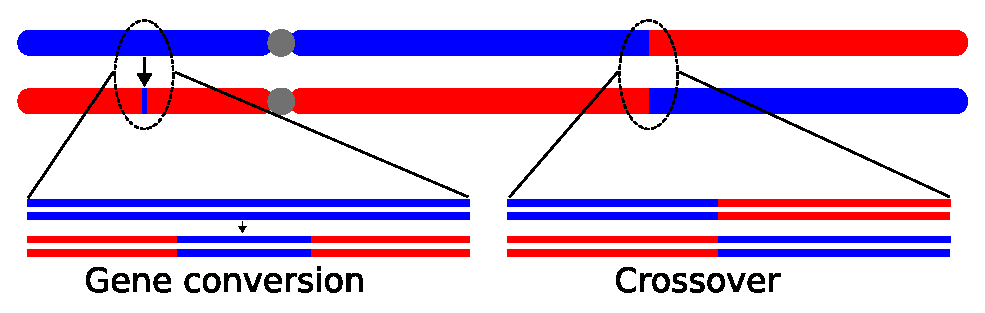
\includegraphics[width=\textwidth]{introduction/figs/outcome_CO-GC}
    \end{center}
    \vspace{-10pt}
    \captionTitle{\textbf{Recombination produces crossover and gene conversion.}}{ 
        Recombination is initiated by DNA double strand breaks that resolve into one of two possible outcomes.
        Crossover (shown at right) is the large-scale, reciprocal exchange of genetic material between two chromosomes around the break point.
        Gene conversion (or non-crossover, shown at left) is the one-way transfer of small amounts of DNA from one chromosome to the other during the repair of the break.
   \label{fig:introOutcomes}}
\end{figure}
\clearpage}


%%%%%%%%%%%%%%%%%%%%%%%%%%%%%%%%%%%%%%%%
\subsection{The biology of meiotic recombination}
%%%%%%%%%%%%%%%%%%%%%%%%%%%%%%%%%%%%%%%%

Prior to meiosis, a diploid cell contains pairs of homologous chromosomes, one of the pair inherited from the father, the other from the mother.
This diploid DNA is replicated just prior to the cell entering the meiotic cycle, in premeiotic S-phase\cite{Bell2002} to generate exact copies of each pair of chromosomes, referred to as sister chromatids.
Meiosis consists of two stages; recombination occurs in the first, meiosis I, while meiosis II sees sister chromatids separate into their respective daughter cells.
Meiosis I is the most complex and lengthy stage, with chromosome pairing, synapsis, and recombination all occurring in succession within prophase I, which is  divided into several sub-stages.

In leptotene (derived from Greek meaning ``thin threads''), changes in chromatin cause the newly replicated chromosomes to form thin individual strands.
Here, the synaptonemal complex (SC), a protein structure that will bind the sister chromatids and their homologues into a tetrad begins to assemble.
The SC consists of a scaffold of proteins that first forms with axial elements that associate with the already paired sister chromatids, solidifying their association.

In the zygotene phase (``paired threads''), pairing between the unraveled DNA begins to occur at regions of homology in a process known as synapsis.
Homologous chromosomes connect to to the SC by transverse filaments, drawing them into the SC structure in a progressive zipper-like mechanism, completing synapsis\cite{Yang2009}.
DNA DSBs occur at this stage (*).

By the pachytene stage (``thick threads''), synapsis, and the SC assembly are fully complete, and the pairs of homologous chromosomes bound within the SC are referred to as a tetrad or bivalent.
Recombination occurs here, mediated by the structure of the SC.
A subset of the DSBs are processed as crossovers, at locations called chiasmata.
The remaining DSBs are repaired through a different pathway, as non-crossovers (gene conversions).

In the diplotene stage (``two threads''), the SC is disassembled, allowing the tetrad to relax slightly.
The homologous chromosomes are still held together at chiasmata locations.

In the final substage of prophase I, diakinesis (``moving through''), the chromosomes condense into visible threads, while the cellular machinery begins to prepare for cell division.
The remaining step of meiosis I are metaphase I, and anaphase I.
Chiasmata, holding the chromosomes together as crossover points are cut, allowing the homologous chromosomes to segregate to their respective cellular poles.

Meiosis II is procedurally similar to mitosis, with different results.
Here, the separation of sister chromatids occurs, producing four haploid gametes.




The recombination process is begun by programmed double strand breaks (DSBs) in the DNA, catalyzed by the protein SPO11, which has a similar function to DNA topoisomerases\cite{DeMassy2013}.
There are two isoforms of \textit{Spo11} in humans, and mice, and a recent study in mice suggests that they may have differing functions, with \textit{Spo11$\beta$} being expressed earlier in meiosis, coinciding with most DSBs occurring on the autosomes.
Male mice with only \textit{Spo11$\beta$} had meiotic defects, with the majority of spermatocytes failing to recombine in the pseudoautosomal region (PAR).
Following this, \textit{Spo11$\alpha$} was found to be expressed later in meiosis, and coincided with DSBs located within the sex chromosomes, including the PAR\cite{Kauppi2011,DeMassy2013}.
This evidence indicates that the initiation of DSBs is a complex, multi-stage process, with autosomal DNA process earlier than DNA from the sex chromosomes.




\paragraph{Non-disjunction and the role of recombination.}
In humans, an estimated 30\% of fertilized eggs have aneuploid chromosomes\cite{Hassold2001}, and evidence suggests that meiotic errors are responsible in many cases.
Non-disjunction, the abnormal segregation of chromosomes, can occur at either of the two cell divisions in meiosis.
Meiosis II non-disjunction typically results from a failure of the sister chromatids to separate.
Meiosis I non-disjunction is thought to involve recombination, either in a failure to resolve chiasmata, or a lack of chiasmata entirely.

A reduced recombination rate has been observed in human genetic maps generated from viable meiosis I aneuploidies (15, 16, 18, 21, XXX, XXY)\cite{Hassold2001,Lynn2004}.
This indicates that recombination rate must remain above a certain level to prevent non-disjunction.
This is supported by the finding that many trisomies involve achiasmate chromosomes, in which recombination is absent in that chromosome(*).

This supports the idea that chiasmata, which serve to tether homolgous chromosomes together after the dissolution of the SC, and through the first, provide a crucial tension that serves to inhibit non-disjunction.
Research suggests that there is a requirement of one chiasma per chromosome to prevent non-disjunction, but that there may be a backup mechanism to enable chromosomes to properly segregate even without any chiamata\cite{Fledel-Alon2009}.



%%%%%%%%%%%%%%%%%%%%%%%%%%%%%%%%%%%%%%%%
\subsection{Timing of meiotic events}
%%%%%%%%%%%%%%%%%%%%%%%%%%%%%%%%%%%%%%%%

%Human:
The fundamental steps of meiosis are the same in males and females, but the timing of these events, both prior and during, differs significantly between the sexes\cite{Lynn2004}, and even between species.
In humans, male meiosis begins at puberty and continues in a cycle that lasts throughout the lifespan.
As male meiosis is continually occurring, the precursor cells undergo a minimum of 30 divisions prior to entering meiosis, and this number continues to rise with age.
A 15 year old male is estimated to be 35 germ-cell divisions, with this number rising to 380 at age 30, and 840 by age 50\cite{Crow2000a}.

Females have 22 cell divisions prior to meiotic entry, and one during, for a total of 23 divisions\cite{Crow2000a}, and this number is fixed for all oocytes.
In females, meiosis begins prenatally, and oocytes progress through the diplotene stage of prophase I before undergoing an arrest period\cite{Hassold2001,Crow2000a}.
This arrest is called the dictyotene stage, or dictyate arrest, and meiosis is frozen at the point the chromosomes have fully synapsed and chiasmata have formed (Figure \ref{fig:introTiming}).
This arrest period ends only upon ovulation, and thus meiosis can be potentially very lengthy, taking one to five decades to complete.
Additionally, while each male meiosis produces four haploid sperm products, female meiosis yields one haploid oocyte contain the majority of the cytoplasm, the remaining meiosis I and II division products produce polar bodies, which contain DNA but typically apoptose\cite{Schmerler2011}.

Male progenitor cells undergo potentially many more mitotic divisions prior meiotic entry.
As the number of mitioc proliferations increases in males, so does the number of mutations accumulated through DNA replication errors.
A recent study using a chimpanzee pedigree estimated that the number of mutations rises linearly with the father's age, with approximately three additional mutations accumulating per year\cite{Venn2014}.
This contributes to a paternal age effect, with mutations accumulating on the male germ line with increasing age.

Dog meiosis differs from that of humans in some key respects.
Meiosis in female dogs begins later, starting in the neonatal period\cite{Freixa1987}.
The meiotic arrest occurs at the same dictyotene stage in both species, but is shorter in dogs, given the later onset of meiosis in dogs as well as a reduced lifespan.
In addition, while meiosis exits the arrest period prior to ovulation in humans, dogs ovulate immature, primary oocytes, which only mature to fertility 48-60 hours after ovulation\cite{Tsutsui1989,Chastant-Maillard2011}.

\afterpage{
\begin{figure}[P]
    \begin{center}
    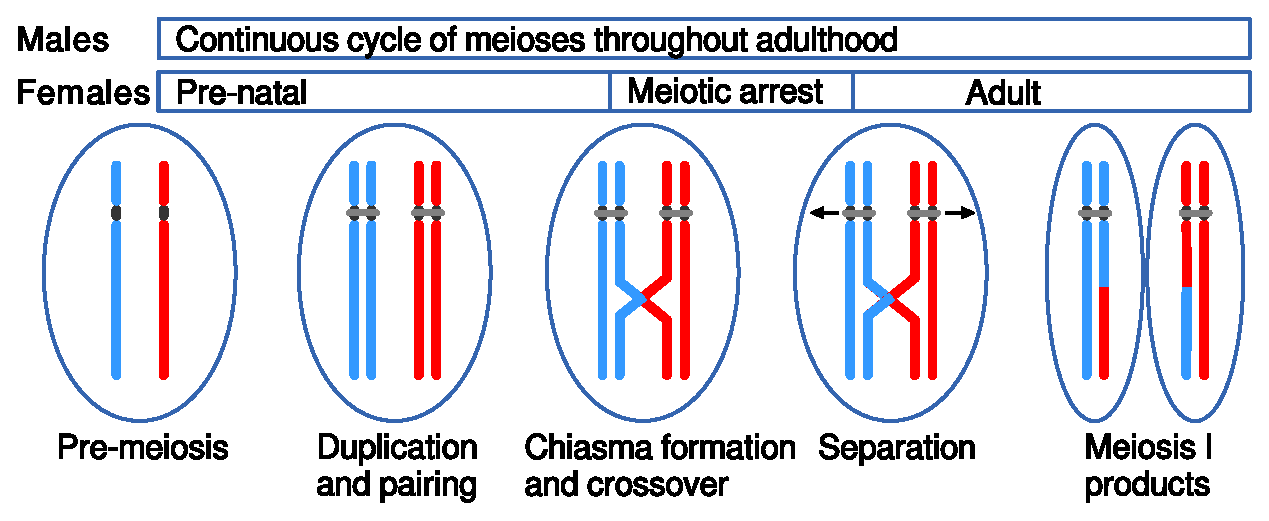
\includegraphics[width=\textwidth]{introduction/figs/meioticTiming}
    \end{center}
    \vspace{-10pt}
    \captionTitle{\textbf{Timing of meiosis I events in humans.}}{ 
        Males exhibit a continuous wave of meioses throughout adulthood.
        In females, meiosis begins before birth and enters an arrest period that can last decades before completion.
   \label{fig:introTiming}}
\end{figure}
\clearpage}

Several biological possibilities have been proposed to explain what happens to oocytes during meiotic arrest.
Polani1991, Rowsey2014: Production line hyp.
Polani: production line holds true for mice



%%%%%%%%%%%%%%%%%%%%%%%%%%%%%%%%%%%%%%%%
%%%%%%%%%%%%%%%%%%%%%%%%%%%%%%%%%%%%%%%%
\section{Historical overview of meiotic recombination}
%%%%%%%%%%%%%%%%%%%%%%%%%%%%%%%%%%%%%%%%
%%%%%%%%%%%%%%%%%%%%%%%%%%%%%%%%%%%%%%%%

% Brief historical review of meiotic recombination, pre Human Genome Project.
Recombination can be observed in a number of ways, and its discovery came decades prior to the discovery of the structure of DNA.
Thomas Hunt Morgan first observed the separation of linked traits while studying Drosophila in 1911\cite{Morgan1911}, and proposed the theory of crossing over between chromosomes.
In addition he suggested that the recombination rate could increase with the distance between factors.
Morgan's student, Alfred Henry Sturtevant, quantified this change in rate over physical distance into ``map distance,'' using this concept to construct the first genetic map.
This map represented the order of, and crossover rates between, genes on the X chromosome in Drosophila\cite{Sturtevant1913}.
In addition, Sturtevant observed that one crossover tended to inhibit the placement of a second nearby, an early description of interference.
A later study by Harriet Creighton and Barbara McClintock in corn (\textit{Zea mays}) in 1931 demonstrated that recombination between genes was tied to an exchange of chromosomal segments\cite{Creighton1931}.

Tracing the inheritance of markers from one generation to the next within a family pedigree provided the first genome-wide measurement of recombination across the human genome, prior to the completion of the Human Genome Project.
Early studies used restriction fragment length polymorphism (RFLP) probes to identify specific loci within the genome, and determine if they are linked.
An early study described the use of RFLPs to generate a linkage map of recombination in the human genome\cite{Botstein1980}.
Further linkage studies increased the marker density across the genome by using microsatellite, short tandem repeat polymorphisms (STRPs) and other approaches to capturing genetic variation\cite{Morton1991,Matise1994,Dib1996}.
The Marshfield map, generated in 1998 by \citet{Broman1998}, was an important step in characterizing recombination on a genome-wide basis.

With the completion of the Human Genome Project and the publication of the draft sequence of the human genome\cite{Venter2001,Lander2001}, human genetic variation has become increasingly well characterized, and a number of technologies have sprung up to make genome-wide ascertainment of variation routine.
Currently, microarray technology provides a well-balanced approach for determining genome-wide coverage of genetic variation.
These arrays target a pre-selected panel of hundreds of thousands to millions of single-nucleotide polymorphisms (SNPs) across every chromosome for a reasonable cost.

%%%%%%%%%%%%%%%%%%%%%%%%%%%%%%
\section{Methods for studying recombination}
%%%%%%%%%%%%%%%%%%%%%%%%%%%%%%

Genome-wide methods have the primary goal of creating a genetic map of the frequency of recombination as a function of physical distance across each chromosome.
In contrast, several other methods are limited in scope, and reveal information about specific loci.
With each method, the detection of recombination is made difficult by the fact that crossovers are rare -- only 20-50 are expected to occur in each meiosis.

% brief introduction to these before describing in detail in "description of approach"

\subsection{Pedigree analysis}

Tracking the transmission of alleles from one generation to the next within known pedigrees provided the first data on recombination in early linkage studies, and pedigree analyses are still in use today.
It is interesting to note that for a pedigree analysis, 
while whole-genome sequencing technology allows the discovery of a higher density of markers across the genome, its use is not typically worth the higher cost.
A higher variant coverage will help to narrow the region of uncertainty surrounding a particular crossover, but it will most likely not assist in the detection of additional crossovers in a single meiosis.

Regardless of the method used for obtaining markers, the principle of detecting recombination in a pedigree remains.
Crossovers can be identified by tracing the allele transmissions from parent to child.
Figure \ref{fig:introPedfig} provides a simple visual example, showing a family quartet.
The father in this pedigree has two informative SNPs producing haplotypes 1-1 and 0-0, while the mother is homozygous at both sites.
The male child has a 1-0 haplotype, and therefore must have inherited a recombinant haplotype from his mother.
We can identify here a crossover event and localize that event to an interval flanked by two informative genetic variants.
This region of uncertainty can vary in size and depends on the spacing and genotypes of polymorphic variants within the genome.
Beyond this intuitive example, the problem of determining the parental phase of a recombinant chromosome has been addressed in a number of methods.
%
\afterpage{
\begin{figure}[p]
    \begin{center}
    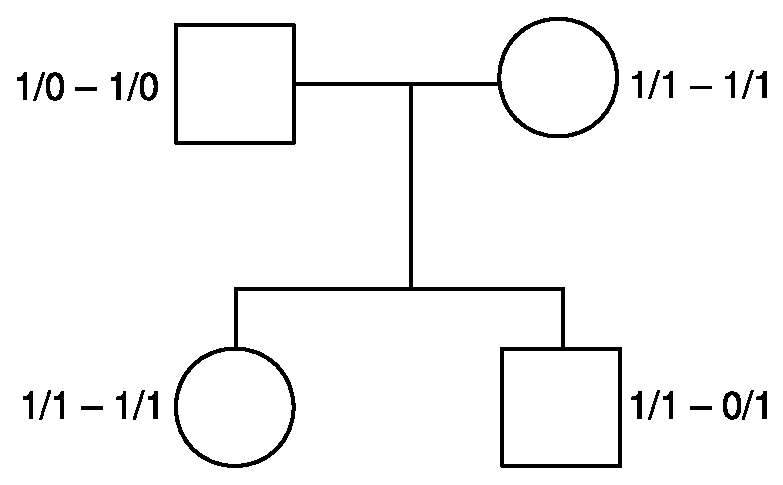
\includegraphics[width=0.75\textwidth]{introduction/figs/pedigree-genotype} \vspace{1cm} \\
    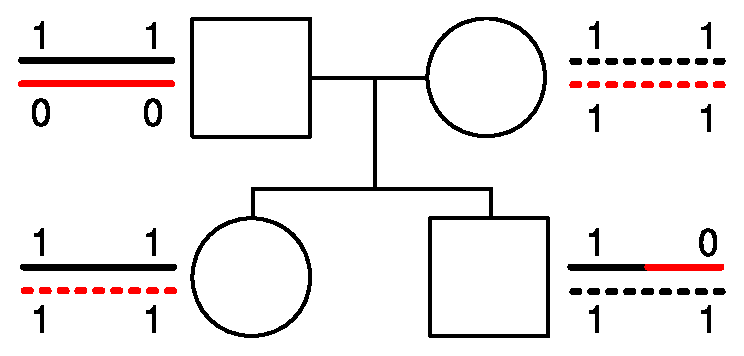
\includegraphics[width=0.8\textwidth]{introduction/figs/pedigree-haplotype}
\end{center}
    \vspace{-10pt}
    \captionTitle{\textbf{Allelic transmission in a family quartet.}}{ 
        The top panel outlines a simple pedigree in which only genotype information is known.
        The bottom panel shows a pedigree for which phase-known haplotype information is known.
        Here, all chromosomes (lines next to each individual) are transmitted in the absence of recombination except for in the male child.  Here there was a recombination event in the father to generate the recombinant chromosome (black/red)
   \label{fig:introPedfig}}
\end{figure}
\clearpage}


\subsection{Linkage disequilibrium approach}

Another powerful method is to use population genetic data to study recombination by inference.
These data can be gathered by genotyping samples of genetic data from unrelated individuals on a microarray or by whole-genome sequencing.

The inference of recombination in such a dataset relies on the quantification of levels of linkage disequilibrium (LD) within the samples, a measurement of linkage between loci.
For example, when alleles at one locus are inherited completely independently of alleles at another locus they are considered to be in linkage equilibrium.
However many alleles exhibit a non-random association, and individuals of the same species tend to share haplotype segments that reflect a shared evolutionary history.
When two alleles on an ancestral haplotype are inherited together they are considered linked, and are not independent of each other.
These alleles exhibit evidence of linkage disequilibrium, a deviation from the assumption of random assortment of alleles.

LD is measured in a pairwise fashion, considering allele frequencies at each pair of markers in the genome.


From measurements of LD within a number of unrelated samples, methods based on coalescent theory have been developed to estimate the recombination rate\cite{Auton2012}.
In software such as LDhat\cite{Mcvean2004,Auton2007,Auton2014}, the population-scale recombination rate, $\rho$, is estimated from the data, and the per-generation recombination rate can be calculated by the relationship
$\rho = 4 N_e r$
where $N_e$ represents the effective population size.
These methods are quite powerful and have produced high-quality estimates of recombination in humans\cite{hapmap2007}, however, they are subject to limitations.
First, that this method requires the knowledge of the genealogical history of a sample, which is unknown, and thus relies on an often simplistic approximation.
Second, these maps by their nature generate sex-averaged data only, since recombination events that are inferred have occurred over the course of potentially thousands of generations.


\subsection{Molecular assays}

A number of molecular assays have been developed for studying recombination.
Most, however are limited to small regions of the genome, and are more effective in males.

\subsubsection{Sperm cell assays}

Sperm typing is one method of identifying both gene conversion and crossover events.
Sperm typing was first used in 1989 to study crossing over in humans\cite{Cui1989}, and uses
allele-specific polymerase chain reaction (PCR) to identify recombination events at a given locus.
In this method, DNA is extracted from multiple haploid sperm cells from a single donor and subject to PCR.
A common reverse primer is used in conjunction with two different allele-specific forward primers, which correspond to polymorphic site in the diploid genome, and are designed to produce different amplicon sizes depending on the matching nucleotide.
Analysis of the PCR products from many sperm cells can reveal the phase of the donor individual, and the recombinant status of each sperm cell.
% \cite{Jeffreys1998,Jeffreys2000,Jeffreys2004}. % first, second(TAP2), review

Sperm typing has been used to produce high-quality data from a number of loci throughout the genome.
One of the first major findings to come out of sperm typing was the characterization of a recombination hotspot in the human major histocompatability complex (MHC), first within one gene, \textit{TAP2}\cite{Jeffreys2000}, then expanded to cover a wider 216 kb region of the MHC\cite{Jeffreys2001}.
All six hotspots found within the region of the MHC were found to be tightly correlated to regions in which LD broke down, providing molecular evidence that recombination hotpots have severe effects on LD patterns.


Jeffreys2009: rise/fall

Berg2010

\citet{Lu2012}
\citet{Wang2012}


\subsubsection{Single oocytes.}
Recent studies have provided much needed insight into recombination in single oocytes through novel methods.
\citet{Hou2013} conducted an analysis in human oocytes, providing at the same time a potential new method for applying next generation sequencing methods to the screening for various genetic disorders with in vitro fertilization (IVF) techniques.
Here, the researchers extracted and fertilized a total of 70 oocytes from 8 Asian female donors, collecting the first and second polar bodies, as well as the male and female pronucleus from the fertilized egg.
This complete collection of data from female oogenesis and fertilization enabled haplotype phasing and crossover calls
Most intriguingly, this enabled the generation of personal genetic maps for each donor, allowing the researchers to address the question of how recombination varies on an individual basis.
This data allows the observation of all four members of the tetrad bundle, both sister chromatids and their homologues, something usually missed by inferential studies of recombination.


Using a similar approach, recovering genetic materiel from the first and second polar bodies and oocyte, \citet{Ottolini2015} were able to observe all four products of female recombination.
The researchers generate ``MeioMaps,'' providing valuable information on how meiosis proceeds on an individual level.



\subsubsection{Recombination initiation maps}
Additional methods have been developed to identify double strand breaks within a individual cells undergoing meiotic recombination.
\citet{Pratto2014} utilized chromatin immunoprecipitation coupled with sequencing to identify DSBs associatated with the strand-exchange protein DMC1 to generate DSB maps in four unrelated human males.
This method identifies the majority of DSBs within the meiotic cell, only a fraction of which will be resolved as crossovers that could be identified via genotyping methods, the remainder ending up as non-crossover gene conversions.
The researchers found the DSB cluster into hotspots, of which 51\% overlapped with the LD crossover hotspots\cite{hapmap2007}, and 80\% of DSB hotspots overlapped regions with elevated recombination rate.
In addition, the DSB locations were largely tied to the specific PRDM9 allele for each particular individual.
PRDM9$_\text{A}$ and PRDM$_\text{B}$ alleles appear to specify similar DSB hotspots, while PRDM9$_\text{C}$ has a separate specificity.
PRDM9 heterozygosity also affects hotspot strength.


% \section{Current ``gold standard'' maps (Hapmap2 LD map, deCODE pedigree map).}
\section{Genetic maps of recombination.}

\subsection{Marshfield map}
The Marshfield map, generated by \citet{Broman1998} in 1998, was the first genetic map of the human genome at a resolution high enough to make inferences on the recombination properties in humans, using $>$8000 short tandem repeat polymorphsims (STRPs) in 188 meioses.
Here, estimates of the genome wide map lengths, inferences on individual variation, and sex differences in recombination were highlighted.
The ratio of female to male autosomal map length was estimated at 1.56, indicating that the recombination rate in females is substantially higher than males.
This ratio has proved stable over a number of studies in the intervening years (summarized in Table \ref{tab:introHeterochiasmy}).
Analysis of this this ratio as a function of chromosome position revealed that male recombination tends to be highest in the telomeres, while females had a higher ratio towards the centromeres.
This study provided valuable insight into sex dimporphism in recombination

\subsection{deCODE maps}
Another major stride in pedigree-based genetic maps came from deCODE genetics, an Icelandic pharmaceutical company that used their database of genealogical and genetic data on many Icelandic families to infer recombination, producing many high quality studies.
The first was in 2002, where 146 families, comprising 1257 meioses, were genotyped using 5136 microsatellite markers\cite{Kong2002}.
This data, in conjunction with the draft sequence of the human genome\cite{Venter2001,Lander2001} was used to improve the marker order and their placement within the reference sequence.
The genetic map generated from this study confirmed much found by \citet{Broman1998} in terms of sex dimorphism in recombination, and further characterized fine scale variation between the chromosomes.
One particular finding was that of recombination ``jungles,'' regions of high crossover rate that clustered towards the telomeres.
In addition, recombination rate was found to correlate with GC content, CpG motif occurrance, and tracts of poly(A)/poly(T), together explaining $\sim$37\% of variation.

In 2010, using genome wide SNP data on x meioses, deCODE genetics published an updated sex-specific recombination map\cite{Kong2010}.
Instead of a typical pedigree-based recombination study, \citet{Kong2010} leverage the high degree of relatedness within the Icelandic population to infer phase and parent-of-origin in 20,217 individuals typed on microarrays assaying $>$289,000 autosomal SNPs.
Here, phase is determined for parent-child pairs by taking into account haplotype blocks that are shared with other individuals within the population to determine the parent-of-origin for a particular block.
Crossovers are called when a segment of a child's haplotype is inferred to move between maternal and paternal origin.
This enables recombination be called in 15,257 parent-offspring pairs.
%%%
One effect of this parent-child phasing approach is that inference of recombination events near the telomeres is difficult, and \citet{Kong2010} omit the most distal 5 Mb for each chromosome.
The omission of the telomeric regions, where male recombination is higher, contributes to the inflation of the female:male map length ratio seen in Table \ref{tab:introHeterochiasmy}) at 1.78 in this study, however much more likely to be closer to the consensus ratio of around 1.56.
Since its release in 2010 the deCODE genetic map has proven quite valuable as a high quality sex-specific map of recombination in the human genome.


\paragraph{Other pedigree studies.}
A study in 2008 employed a pedigree analysis of individuals from the Hutterite population, all of European descent\cite{Coop2008}.
This was the first study to use genome-wide high-density SNP arrays (in this case the Affymetrix GeneChip Mapping 500k array) to study recombination.
A total of 728 meioses were analyzed, yielding valuable data regarding the overlap of crossovers and hotspots on an individual basis.


Other pedigree studies include a map generated from 980 meioses using individuals of Korean and Mongolian descent\cite{Bleazard2013}.

\subsection{Linkage disequilibrium based maps}

LD has been used to great effect in the identification of recombination events, both in the human genome and in other species.
Perhaps the most high-quality LD map comes from data generated from the International Hapmap Project, Phase II\cite{hapmap2007}, which includes data from 270 individuals genotyped at over 3.1 million SNPs.
This map was generated using samples from both European (CEU) and African (YRI) origin, greatly improving the resolution over the Phase I map.
The resolution of this map refined the collection of hotspots first identified by \citet{Myers2005}, and expands this set to include more than 30,000 within the human genome.
This map remains in common use today, still providing the highest resolution of sex-averaged recombination rate across the human genome.


Kong2010 (place elsewhere):
Lower rec. rate within genic regions (and this difference is greater for females).
Recombination tends to be depressed within geneic regions overall compared to intergenic, with recombination high just upstream of the TSS and downstream of the TSE, and falling off after a few hundred kb\cite{Kong2010,Coop2008}.
Additionally, while females have a lower rates within genic regions, males have higher rate within exonic regions.
%%%
% \citet{Coop2008} found that recombination was elevated upstream of the TSS and 




\afterpage{
\begin{table}[p] \centering
    \begin{tabular}{|l|c|c|c|c|c|c|c|} 
        \hline Species & Common name & Study & Year & Female (cM) & Male (cM) & Ratio & Sex avg.\ (cM) \\ \hline
    \hline \end{tabular}
    \captionTitle{\textbf{Autosomal map length estimates for a number of studies in various species.}}{
    Total map lengths are given in centimorgans, while the ratio represents the female to male map lengths. Sex specific map lengths are not available for the LD based maps.\label{tab:introHeterochiasmy}}
\end{table}
\clearpage}



%%%%%%%%%%%%%%%%%%%%%%%%%%%%%%
%%%%%%%%%%%%%%%%%%%%%%%%%%%%%%
\section{Sexual dimorphism in recombination.}
%%%%%%%%%%%%%%%%%%%%%%%%%%%%%%
%%%%%%%%%%%%%%%%%%%%%%%%%%%%%%
\subsection{Heterochiasmy}

The Marshfield map\cite{Broman1998}, provided some of the first evidence of recombination rate variation across the human genome, and between males ane females.
Particularly interesting was the finding that recombination rates are higher in the telomeres, especially in males, and that females have a 1.6-fold higher rate of recombination in the autosomes.
The estimation of this ratio proved to be accurate, despite the low marker coverage and few meioses used, and has been reinforced through numerous follow-up studies\cite{Broman2000,Kong2002,Coop2008,Kong2010,Bleazard2013,Campbell2015,Bherer2016}.

This example in humans provides an illustration of heterochiasmy, the unequal distribution of recombination rates between the sexes of a species.
Humans are among a large majority of species with data currently available in which the female recombination rate is higher than that of the male (Table \ref{tab:introHeterochiasmy}).


Haldane-Huxley rule: when recombination is absent in one sex, it is the heterogametic sex.
%
Trivers hypothesis: recombination is lower in the sex that undergoes stronger selection (recombination disrupts favorable haplotypes in the most fit individuals, therefore is selected against).


\paragraph{Distribution.}

\paragraph{Differences in SC lenth.}

\subsection{Recombination under genetic control}
% Genes involved in recombination (RFN212, etc)}

A number of genetic factors have been identified that alter properties of recombination, a summary of which can be found in Table \ref{tab:introGenes}.

In a sperm typing analysis, \citet{Jeffreys2005} found a SNP whose minor allele suppressed the ratio of crossover to gene conversion near a particular hotspot.
Additionally, this variant was found to be overtransmitted, an example of meiotic drive.
Another study in the Icelandic population found an association with an inversion at 17q21.31 on recombination rate\cite{Stefansson2005}.
The presence of this inversion is associtated with an increase in crossover rate in females, but not males.

% RNF212: indentified in Saccharomyces cerevisiae and Caenorhabditis elegans
RNF212 has been associated with recombination rate in an Icelandic population\cite{Kong2008}, and this has been replicated in a number of follow-up studies\cite{Chowdhury2009,Fledel-Alon2011,Reynolds2013,Kong2014}.
Interestingly, the linkage of two particular SNPs near this gene is associated with an increased recombination rate in males, and a corresponding low rate in females.
RNF212 is a homologue of ZHP-3, a \textit{C.\ elegans} gene involved in crossing over and disjunction, localizing to sites of crossover, and aids in the change in chromatin structure that occurs with the disassembly of the synaptonemal complex\cite{Bhalla2008}.
Mouse RNF212 was found to have similar function, facilitating synapsis, and forming crossover-stabilizing structures\cite{Reynolds2013}.
%Rnf212 KO mice are sterile but achieve complete synapsis.
In addtion RNF212 possibly influences the decision to repair a DSB as a crossover rather than a gene conversion\cite{Reynolds2013}.
RNF212 has also been shown to associate with recombniation rate in cattle\cite{Sandor2012}.

A study by \citet{Chowdhury2009} using 2310 meioses found significant associations with variants associated with four gene regions.
Two were associated with female recombination rate (KIAA1462, PDZK1), and the other two with male rate (UGCG, NUB1).
These genes are poorly characterized and their function, beyond potential meiotic roles, remains unknown.
However, this study reinforces the suggestion that male and female recombination rate are controlled via differing genetic factors.

Another study, again in the Icelandic population with an expanded number of meioses, identified a further 8 genomic regions that have separate associations with male and female rates\cite{Kong2014}.
In the telomeric region of chromosome 4, near RNF212, one variant was found that was estimated to increase the map length by 386 cM in females, and 124 cM in males.
Novel variants were found in an additional six genes (Table \ref{tab:introGenes}).

The strongest association thus far has been with PRDM9, which was first associated with hotspot usage and variation in alleles encoding the zinc finger array by \citet{Baudat2010}.
Baudat2010 (Association with hotspot usage and zn finger alleles)
Berg2010 (Sperm typing to determine that Zn finger array variation leads to differences in hotspot usage)
Berg2011
Hinch2012(
Kong2010: PRDM9 confirmation phenotype association


Additionally, REC8 has been shown to influence recombination rate in male cattle\cite{Sandor2012}.

\afterpage{
\begin{table}[p] \centering
    \small
    \begin{tabular}{|l|c|c|p{1.3cm}|p{1.3cm}|c|c|} 
\hline Gene / region & Chr. & Association & Female rate & Male rate & Study & Replication \\ \hline
        RNF212 & 4 & rate & + & - & \citet{Kong2008} & \cite{Chowdhury2009,Fledel-Alon2011,Reynolds2013,Kong2014,Campbell2015} \\
        17q21.31 inversion & 17 & rate & + & none & \citet{Stefansson2005} & \cite{Fledel-Alon2011,Chowdhury2009,Kong2014} \\
        KIAA1462 & 10 & rate & + & none & \citet{Chowdhury2009} &  \\
        PDZK1 & 1 & rate & + & none & \citet{Chowdhury2009} &  \\
        UGCG & 9 & rate & none & + & \citet{Chowdhury2009} &  \\
        NUB1 & 7 & rate & none & + & \citet{Chowdhury2009} &  \\
        CCNB1IP1 & 14 & rate & + & weakly + & \citet{Kong2014} & \cite{Campbell2015} \\
        C14orf39 & 14 & rate & + & none & \citet{Kong2014} &  \\
        SMEK1 & 14 & rate & + & none & \citet{Kong2014} & \cite{Campbell2015} \\
        RAD21L & 20 & rate & weakly + & + & \citet{Kong2014} &  \\
        MSH4 & 1 & rate & + & none & \citet{Kong2014} &  \\
        CCDC43 & 17 & rate & + & none & \citet{Kong2014} &  \\
        PRDM9 & 5 & hotspot usage & NA & NA & \citet{Baudat2010} & \cite{Fledel-Alon2011,Campbell2015,Kong2014} \\
    \hline \end{tabular}
    \captionTitle{\textbf{Genomic regions associated with recombination in humans.}}{
    \label{tab:introGenes}}
\end{table}
\clearpage}




%%%%%%%%%%%%%%%%%%%%%%%%%%%%%%%%%%%%%%%%
\subsection{Determinants of recombination placement (PRDM9, GC, chromosome position).}
%%%%%%%%%%%%%%%%%%%%%%%%%%%%%%%%%%%%%%%%

Differences in populations (Berg2010,Berg2011,Hinch2011)

\subsection{Heritability of recombination modifiers}

The 2004 deCODE study, by analyzing siblings in large families, suggested that recombination rates were broadly heritable\cite{Kong2004}.
The pedigree analysis of the Hutterize population by \citet{Coop2008} was the first to find extensive variation among individuals in terms of their hotspot overlap (the proportion of an individual's crossover that overlap with known hotspots).
Another significant finding was that hotspot overlap was heritable.
This raises the possibility that other aspects of the recombination process may also be heritable.
And supports previous data from sperm typing finding that a hotspot-proximal SNP had recombination-suppressing effects, and that this SNP is over-transmitted to progeny\cite{Jeffreys2005}.

A follow-up study in 2011 reinforced the heritability of hotspot usage as a phenotype, and expanded the scope\cite{Fledel-Alon2011}.
This study found that both male and female recombination rates are heritable.
Additionally, associations with RNF212 and the inversion on 17q21.31 were replicated.


% Ottolini2015: selection for maternal recombination rates. (Kong2004 suggested this as well).
%\section{Heritance of recombination modifiers (rate, etc. Kong)}

%%%%%%%%%%%%%%%%%%%%%%%%%%%%%%
\subsection{Maternal age effect.}
%%%%%%%%%%%%%%%%%%%%%%%%%%%%%%

Age effects on reproduction have been tied with an increased incidence of aneuploidy in humans\cite{Hassold2001,Hassold2007}.

Several studies have shown evidence for an increase in the number of crossover events with maternal age, suggesting a protective mechanism against aneuploidy.
%%%
With the aim of investigating age effects in recombination, a study in 2004 using the deCODE genetics dataset with 23,066 meioses, using a reduced set of 1000 microsatellite markers\cite{Kong2004}.
Genotyping was not done for every individual, with some families having only one parent genotyped, and recombination events were therefore imputed.
The main finding from this study is that the number of crossovers observed in females appears to increase with age, with an additional 0.082 events per year ($\pm$0.012), corresponding to a 4\% increase over 25 years.
This effect was seen to increase within families, such that a child born later in the mother's life has a higher number of maternal crossover than their siblings born earlier.
\citet{Coop2008} analyzed recombination in 728 meioses from Hutterites, and found that mothers 35 year or older have an extra 3.1 crossover events compared to mothers under 25 years old.
This effect corresponds with an extra 0.19 events per year ($\pm$0.092).
No such effect was found in males in either study.
%%%

A study by \citet{Hussin2011} examined in recombination in 195 maternal meioses from French-Canadian pedigrees.
Here, the opposite effect was seen, with recombination rate found to decrease with maternal age, with a larger effect size, estimating a decrease somewhere between $-$0.49 and $-$0.42 events each year.
Differences in the direction of the effect here may be due to real differences between populations, when considering the French-Canadian as a genetic isolate, or simply due due to a lack of power with only 195 meioses.
%%%
Another study reported a slight decrease in crossover count with maternal age in 338 meioses, finding a decrease of $-$0.29 events per year\cite{Bleazard2013}.
In a direct test of the production line hypothesis, \citet{Rowsey2014} examine more than 8000 oocytes, finding no significant change in crosover count among oocytes.
Thus, it appears that the number of crossovers in a given oocyte is not governed as a function of order of meiotic entry, and there is a lack of evidence for any effects of the production line hypothesis on crossover count.

While evidence for an age effect on crossover count in females is conflicting, these studies all agree that there is no age effect present in males.
A recent meta-analysis by \citet{Martin2015} provided much need insight into the age effect issue.
Using a combination of nine cohorts comprising $>$6000 meioses, the authors report a modest but significant increase in the crossover count with age.
The authors used a comprehensive and systematic approach that avoids the methodological differences between previous studies.
%%%
An interesting suggestion from this study, was that of possible confounding factors upon the maternal age effect.
One, that assisted reproductive technologies, including IVF, may provide an artificial selection for oocytes with a greater number of crossovers.
Second was the possibility that oral contraception, which suppresses ovulation, could somehow alter the age-count association, especially if the production-line hypothesis holds true for humans.
However, neither of these possibilities could be controlled for with the power of this study and remain undetermined.


Additional evidence from an analysis of single oocytes provides evidence that maternal recombination rate is highly variable within a single individual, with 41.6 $\pm$ 11.3 crossover per oocyte\cite{Ottolini2015}.
This study revealed a selection against transmission of non-recombinant oocytes at meiosis II, which were more likely to be found in the second polar body instead of the transmitted oocyte.
This evidence outlines a potential mechanism by which non-recombinant, potentially aneuploid oocytes could be eliminated from the germ line.
Furthermore, recombination, thought to be limited to prophase I, was shown to influence events in meiosis II, much later than previously thought.

\section{Recombination in other organisms, including dogs.}


Recombination in humans is of great interest to us as a species, and much effort has been focused here.
However it is of great interest to learn about recombination in all species to put human recombination in an evolutionary context.
Studies of recombination have been done in a wide variety of organisms to date, a partial list of which is summarized in Table \ref{tab:introHeterochiasmy}.

Chimpanzees, the most recent common ancestor to humans, have a LD-based recombination map\cite{Auton2012a}, but no pedigree maps are yet available, leaving open questions regarding sex differences.

Pedigree maps have been generated in mice\cite{Broman2002}, the most recent of which 
was generated by \citet{Cox2009}, using 3546 meioses, but a low density of markers.
More recently, data from the Collaborative Cross(citation), an inbred population generated from eight founder strains, has been used to generate sex-specific maps within the mouse genome\cite{Liu2014}.
The researchers here leveraged the breeding funnel approach from the Collaborative Cross, gathering genotype data from sibling pairs, and using computational techniques to infer recombination events.


Yeast has been the subject of a number of studies, due to their ease of use as a model organism and much of what we know today comes from yeast.

Recombination maps are available in a number of other species, but most are limited to LD studies, due to the steep resource requirements of pedigree studies.
Most recently, study of recombination was released in yeast\cite{Lam2015} and birds\cite{Singhal2015}.
These studies provided an evolutionary perspective on recombination initiation and hotspot evolution.


%%%%%%%%%%%%%%%%%%%%%%%%%%%%%%%%%%%%%%%%
\section{Hotspots}
%%%%%%%%%%%%%%%%%%%%%%%%%%%%%%%%%%%%%%%%

\subsection{Initial discovery of hotspots}

Sperm typing produced the first set of well-characterized hotspots in humans, initially focusing within the MHC\cite{Jeffreys2000,Jeffreys2001}.
The correlation of hotspot locations identified by sperm typing in this regions with breakdown of LD measurements provided support for the use of LD methods to find hotspots of recombination genome-wide, without the expense and limitations of single-cell assays\cite{Jeffreys2001}.
In 2005, \citet{Myers2005} produced a fine-scale recombination map in the human genome using LD methods.
Along with this map, hotspots were found to be a ubiquitous feature of the human genome, with a set of $\sim$25,000 found, occurring roughly every 50 kb.
Hapmap LD study expand characterized hotspots throughout the human genome.
These LD studies of recombination also estimated the proportion of recombination occurring within various fractions of the total genome sequence, finding that recombination was intensely concentrated, with 80\% of all recombination occupying less than 20\% of sequence.

Extensive analysis by sperm typing has indicated that hotspots are generally 1-2 kb in width\cite{Jeffreys2004a,Arnheim2003}.


\subsection{Discovery of PRDM9}

Since hotspots were first looked at in detail, and the discovery that they were common and spread across the entire genome, questions regarding a possibly regulatory mechanism for hotspots have persisted.
\citet{Myers2005} found that hotspots shared many common features including repeat elements THE1A/B, and a common sequence motif (CCTCCCT) located at the centers of many hotspots.
A further famly of motifs were identified via the use of the Hapmap phase 2 LD map\cite{hapmap2007}, encompassed by the degenerate 13 bp motif (CCNCCNTNNCCNC)\cite{Myers2008}, estimated to be involved in up to 40\% of all hotspots.

Spencer2006 : hotspots associated with increased GC content, and GC increasing mutations, a likely result of the action of biased gene conversion.


In 2010, a series of papers by three separate groups converged on the identification of PRDM9 from different approaches.
This protein, originally called \textit{Meisetz} was discovered in mice, and is active in early meiotic prophase\cite{Hayashi2005}.
PRDM9 contains a high polymorphic zinc finger DNA binding array, as well as a methyltransferase domain, responsible for the trimethylation of lysine 4 on histone 3 (H3K4).

\citet{Myers2010} compared the sequence of the 13 bp motif against predicted binding of various zinc finger arrays in the genome, finding PRDM9 as a top candidate.
%predicted binding sequence of the PRDM9 zinc-finger array in humans, they found that PRDM9 is a match for the 13 bp sequence motif found at the center of human hotspots.
%Looked at the recombination rate in chimpanzees in sequence surrounding human hotspotso
Using a mouse genetic approach, \citet{Baudat2010} focused on a locus previously determined to be involved in localization of crossover initiation\cite{Grey2009,Parvanov2009},
and narrowed this genomic interval to a region containing the \textit{Prdm9} gene.
A third study used fine mapping techniques in mice to narrow the region, again identifying PRDM9 as the likely candidate protein\cite{Parvanov2010}.

\subsection{PRDM9 alleles}

The PRDM9 zinc finger array has tremendous variability and there are a number of alleles present.
The major alleles A and B, are both present in a high percentage of European individuals, and differ by only a single amino acid change\cite{Baudat2010}.
The A and B alleles are predicted to recognize the degenerate 13-mer motif, but the I allele is not\cite{Baudat2010}.
This effect is seen at the DSB-level as well, with PRDM9 A and B variants contributing to generate silmilar DSB hotspots\cite{Pratto2014}.

Furthermore the PRDM9 allele status of an individual has a strong effect on the hotspot overlap.
In the Hutterite study, A/A individuals have significantly different overlap compared to A/I, and A/B, with the A/I heterozygous having lower hotspot usage overall\cite{Baudat2010}.


Sperm typing in men of African ancestry revealed that PRDM9 variants similar to the ``C'' allele (termed C-type), were more common in this population.
Furthermore, these C-type alleles specified different hotspots with a motif different from those seen Europeans\cite{Berg2011}. 
These ``African-enhanced hotspots'' all contained a common motif, CCNCNNTNNNCNTNNC, but were associated with the PRDM9 C-type alleles.




\subsection{Hotspots in other species}

Hotspots have been discovered in a number of other species.

Mice contain approximately 15,000-20,000 hotspots, also under the regulation of PRDM9
Mice: Brick2012 (Hotspots via ChIP); Smagulova2011. 15-20,000 total

PRDM9 absent / present

Dogs (Axelsson, Auton2013)

Yeast

Birds


\subsection{Conservation between species}

Humans and chimpanzees have a complete absence of hotspot sharing, despite a high degree of overall DNA sequence identity\cite{Ptak2005,Winckler2005,Auton2012a}.

Evidence points the rapid evolution of the zinc finger DNA binding array as an explanation for the lack of shared hotspots between humans and chimpanzees\cite{Myers2010}, and a wide variety of mammals\cite{Oliver2009,Ponting2011,Thomas2009}.

Discuss hotspot paradox vs stable hotspots theory (latter saying hotspots are confined to specific chromosome features (promoters/GC content), as in yeast and dogs)

\subsubsection{Species lacking PRDM9}
Dogs, birds (Singhal2015, biorxiv) 

\section{Recombination and disease}

The most direct association of recombination with disease is the association with aneuploidy due to meiosis I errors\cite{Hassold2001,Hassold2007}.
As recombination has such a high impact on the structure of the genome, it also has the possibility to cause genomic instability if errors occur during the break and repair of DNA.
Defects in recombination have been associated with a number of disorders caused by genomic instability.
Nonallelic homologous recombination (NAHR), also known as ectopic exchange results in structural genomic rearrangements and is a major cause of recombination-associated copy number alteration.
For example, 22q11.2 deletion syndrome is believed to be caused by improper pairing and crossing over between low copy repeats (LCRs) that flank the region, causing it to be deleted in the recombinant chromosome\cite{Emanuel2008}.
Ectopic exchange contributes to a number of other diseases associated with genomic rearrangements\cite{Stankiewicz2002,Liu2012}.
\citet{Berg2010} reported that variation found at the PRDM9 locus contributed to genome instability.
\citet{Pentao1992} found that rearrangements between repeat regions associate with the the deleteion of a 1.5 Mb region, associated with Charcot-Marie-Tooth disease type 1A (CMT1A).
Deletion of the 7q11 region in sperm causes Williams-Beuren syndrome\cite{Turner2008}.

PRDM9 has also been implicated in genomic instability associated disease.
PRDM9 hotspot motifs have been found in regions associated with disorders of genomic instability\cite{Myers2008}.
In a sperm-typing study, non-A alleles of PRDM9 were found to be protective against the risk of rearrangements leading to CMT1A and hereditary neuropathy with liability to pressure palsies (HNPP)\cite{Berg2010}.
Here, a protective effect against genome rearrangement was seen in men homozygous for the N/N allele, with a lesser effect in heterozygous A/N individuals.

In addition, PRDM9 has been associated with children with B-cell precursor acute lymphoblastic leukemia (B-ALL)\cite{Hussin2013}.
Here, a rare PRDM9 allele (C) was found in a number of families, and was tied to the abnormal X of crossover events, and associated with B-ALL.

Berg2011:

However, an interesting recent study identified a healthy mother carrying a homozygous knockout of PRDM9 predicted to render the protein inactive\cite{Narasimhan2016}.
In PRDM9 knockout mice, meiosis is not able to complete properly\cite{Brick2012}.
However, this mother had three healthy children, one of which carried the mutation.
In this transmission, crossovers at PRDM9 binding locations reduced in number.
This observation by \citet{Narasimhan2016} raises the possibility of a backup mechanism for the completion of meiosis in the absence of PRDM9 in the human genome.

%%%%%%%%%%%%%%%%%%%%%%%%%%%%%%%%%%%%%%%%
%%%%%%%%%%%%%%%%%%%%%%%%%%%%%%%%%%%%%%%%
\section{Crossover interference}
%%%%%%%%%%%%%%%%%%%%%%%%%%%%%%%%%%%%%%%%
%%%%%%%%%%%%%%%%%%%%%%%%%%%%%%%%%%%%%%%%

% Current status of crossover interference field.
\begin{titemize}
    \item gamma and two-pathway model, math review.
    \item other methods of measuring coint
    \item genetic map functions taking into account coint Speed,Zhao
    \item potential method of coint action.
    \item Cover what's known in humans, dogs, other organisms.
\end{titemize}



The crossovers identified from single oocytes by \citet{Hou2013}
allows valuable data to be inferred regarding both crossover interference, affecting the spacing between pairs of crossovers.
Comparing to previously published sperm data\cite{Lu2012}, \citet{Hou2013} look at crossover spacing as a function of both physical distance (in bp), and synaptonemal complex length (\SI{}{\micro\metre}), concluding that the strength of interference is equivalent in males and females when considering the synaptonemal complex length, which is longer in females, reflecting their higher recombination rate.
%an observation that conflicts with a number of other studies\cite{Broman2000,Housworth2003,Fledel-Alon2009}.
Somewhat puzzling was the omission of genetic distance (in centimorgans) in this analysis, a factor that controls for the 1.6 fold higher recombination rate in females over males.
A reanalysis of this data using genetic distance is presented in this thesis in Chapter X.

%%%%%%%%%%%%%%%%%%%%%%%%%%%%%%%%%%%%%%%%
\subsection{Chromatid interference}
%%%%%%%%%%%%%%%%%%%%%%%%%%%%%%%%%%%%%%%%

Another type of interference that is somewhat more difficult to observe, and therefore less studied, is chromatid interference.
Chromatid interference affects which chromatid is involved in crossing over within the tetrad.

By identifying which chromatid is involved in each crossover \citet{Hou2013} found evidence for weak and negative chromatid interference in human oocytes.
This means that once an initial crossover is established between two chromatids (e.g.\ labeled 1 and 2), a second crossover is more likely to form using at least one of these first chromatids (1 and 2), and less likely to form using neither (between 3 and 4).
Positive chromatid interference corresponds to an decrease in the probability of a second crossover involving the same chromatids as the first, that is, the first crossover ``interferes'' or prevents the placement of the second on the same chromatids.

In another study, \citet{Fledel-Alon2009} used the observed crossovers to infer the chiasma count in tetrads using human pedigrees.
Under their model, chromatid interference could account for the observed transmission of nullichiasmic, non-recombinant chromatids, however there was not enough evidence to conclude this definitively.

% However, evidence for chromatid interference has been found in yeast\cite{Zhao1995}


%%%%%%%%%%%%%%%%%%%%%%%%%%%%%%%%%%%%%%%%
%%%%%%%%%%%%%%%%%%%%%%%%%%%%%%%%%%%%%%%%
\section{Gene conversion}
%%%%%%%%%%%%%%%%%%%%%%%%%%%%%%%%%%%%%%%%
%%%%%%%%%%%%%%%%%%%%%%%%%%%%%%%%%%%%%%%%

\begin{titemize}
    \item Review of Li \& Stephens and other models
    \item HMM
    \item Williams paper
\end{titemize}

%%%%%%%%%%%%%%%%%%%%%%%%%%%%%%%%%%%%%%%%
%%%%%%%%%%%%%%%%%%%%%%%%%%%%%%%%%%%%%%%%
\section{Hypothesis and goals}
%%%%%%%%%%%%%%%%%%%%%%%%%%%%%%%%%%%%%%%%
%%%%%%%%%%%%%%%%%%%%%%%%%%%%%%%%%%%%%%%%

% Hypothesis / goal of this thesis.
\begin{titemize}
    \item To investigate specific properties of recombination and how it differs between sexes, individuals, populations, and species.
        %\item To examine how the absence of PRDM9 has affected the recombination landscape in dogs.
    \item To examine how crossover interference varies between individuals and across species.
    \item To further investigate possibilities to model gene conversion in the human genome.
\end{titemize}

%%%%%%%%%%%%%%%%%%%%%%%%%%%%%%%%%%%%%%%%
%%%%%%%%%%%%%%%%%%%%%%%%%%%%%%%%%%%%%%%%
\section{Description of approach}
%%%%%%%%%%%%%%%%%%%%%%%%%%%%%%%%%%%%%%%%
%%%%%%%%%%%%%%%%%%%%%%%%%%%%%%%%%%%%%%%%

% Description of approach.
\subsection{Methods used here to study recombination}
Here, I outline the methods used to study recombination in humans and dogs.

\subsubsection{Linkage disequilibrium}


\subsubsection{Pedigree analysis}

\paragraph{Lander-Green algorithm.}
\paragraph{SHAPEIT2/duoHMM.}

\subsection{Models of crossover interference}
    Models of crossover interference (described in full in nat comm paper).

\subsection{Gene conversion HMM}
    Gene conversion in admixed populations HMM \& statistical methods for recombination modeling.


%%%%%%%%%%%%%%%%%%%%%%%%%%%%%%%%%%%%%%%%
%%%%%%%%%%%%%%%%%%%%%%%%%%%%%%%%%%%%%%%%
\clearpage
\renewcommand{\bibname}{References}
\bibliographystyle{ccampbell_thesis} %unsrtnat} %abbrvnat_noURL} %abbrvUnsrt_last-first} %plain,unsrt,alpha,abbrv,acm,apalike,unsrt
\begingroup
    \setlength{\bibsep}{10pt}
    \linespread{1}\selectfont
    \bibliography{/home/ccampbell/Dropbox/papers/recombination,/home/ccampbell/Dropbox/papers/thesis}
\endgroup
%%%%%%%%%%%%%%%%%%%%%%%%%%%%%%%%%%%%%%%%
%%%%%%%%%%%%%%%%%%%%%%%%%%%%%%%%%%%%%%%%


%%%%%%%%%%%%%%%%%%%%%%%%%%%%%%

%%%%%%%%%%%%%%%%%%%%%%%%%%%%%%
\begin{SingleSpace}
\chapter{Escape from crossover interference increases with maternal age} \label{ch:cointEsc}
%%%%%%%%%%%%%%%%%%%%%%%%%%%%%%

\noindent Christopher L. Campbell$^1$, Nicholas A. Furlotte$^2$, Nick Eriksson$^{2,\dagger}$, David Hinds$^2$, and Adam Auton$^1$

\vspace{0.5cm}
\noindent This manuscript has been published: \\
Campbell, C. L. et al. Escape from crossover interference increases with maternal age. Nat. Commun. 6:6260 doi: 10.1038/ncomms7260 (2015). \\
PMCID: PMC4335350

\vspace{0.5cm}
\noindent $^1$ Department of Genetics, Albert Einstein College of Medicine, 1301 Morris Park Avenue, Bronx, New York 10461, USA. \\
\noindent $^2$ 23andMe Inc., Mountain View, California 94043, USA. \\
\noindent $^\dagger$ Present address: Coursera, 381 East Evelyn Avenue, Mountain View, California 94041, USA. \\

\vspace{0.5cm}
\begin{centering}
    Correspondence and requests for materials should be addressed to \\
    A.A.\ (email: \texttt{adam.auton@einstein.yu.edu}). \\
\end{centering}
\end{SingleSpace}

%%%%%%%%%%%%%%%%%%%%
% \DoubleSpacing

\begin{abstract}

Recombination plays a fundamental role in meiosis, ensuring the proper segregation of
chromosomes and contributing to genetic diversity by generating novel combinations of
alleles. Here, we use data derived from direct-to-consumer genetic testing to investigate
patterns of recombination in over 4,200 families. Our analysis reveals a number of sex
differences in the distribution of recombination. We find the fraction of male events occurring
within hotspots to be 4.6% higher than for females. We confirm that the recombination rate
increases with maternal age, while hotspot usage decreases, with no such effects observed in
males. Finally, we show that the placement of female recombination events appears to
become increasingly deregulated with maternal age, with an increasing fraction of events
observed within closer proximity to each other than would be expected under simple models
of crossover interference.

\end{abstract}


%%%%%%%%%%%%%%%%%%%%%%%%%%%%%%%%%%%%%%%%
%%%%%%%%%%%%%%%%%%%%%%%%%%%%%%%%%%%%%%%%
\section{Introduction}
%%%%%%%%%%%%%%%%%%%%%%%%%%%%%%%%%%%%%%%%
%%%%%%%%%%%%%%%%%%%%%%%%%%%%%%%%%%%%%%%%

Recombination is a fundamental meiotic process that is
required to ensure the proper segregation of chromosomes.
In mammals and other eukaryotes, at least one crossover is
normally required to ensure proper disjunction, and failures in
recombination can result in deleterious outcomes such as
aneuploidy. As such, the recombination process is highly
regulated to ensure that sufficient numbers of crossovers occur.
The placement of crossover events along a chromosome is also
tightly regulated. At the fine scale, the majority of crossovers tend
to occur within localized regions of $\sim$2 kb in width known as
recombination hotspots. At broader scales, interference between
crossovers appears to increase spacing between events occurring
on the same chromosome during meiosis.

As relatively few crossover events occur within a single meiosis,
quantifying the recombination landscape requires the observation
of large numbers of meioses. In this study, we adopt a pedigree
approach to study the properties of recombination in over 18,000
meioses using data derived from families genotyped via 
direct-to-consumer genetic testing. Our approach enables hundreds of
thousands of recombination events to be localized, and allows us
to investigate how the frequency and placement of recombination
changes as a function of sex and parental age.

%%%%%%%%%%%%%%%%%%%%%%%%%%%%%%%%%%%%%%%%
%%%%%%%%%%%%%%%%%%%%%%%%%%%%%%%%%%%%%%%%
\section{Results}
%%%%%%%%%%%%%%%%%%%%%%%%%%%%%%%%%%%%%%%%
%%%%%%%%%%%%%%%%%%%%%%%%%%%%%%%%%%%%%%%%

To investigate properties of crossover placement in humans, we
collected data from pedigree families contained within the
database of 23andMe Inc. (Mountain View, CA). Our data set
consists of 4,209 families contributing a total of 18,302
informative meioses genotyped at over 515,972 sites. To preserve
the privacy of the participants, families were removed if the age of
the mother was greater than 40 years at the time of childbirth,
the age of the father was greater than 45 years or the difference
between the parental ages was greater than 15 years
(Supplementary Fig. \ref{fig:cointFS1}). The majority of the data is derived from
family quartets (Supplementary Table \ref{tab:cointTS1}), accounting for 78.6\% of
the families, and is also predominately composed of individuals of
European ancestry (Supplementary Table \ref{tab:cointTS2}). Ancestral populations
are assigned to each individual by comparison with a set of
reference populations (see Supplementary Methods).

To infer recombination events in nuclear families, we applied
the Lander-Green algorithm as implemented within \citet{Abecasis2002}.
To guard against genotyping error, we curated the data to remove
nearby recombination events that could be indicative of
genotyping error (see Supplementary Methods; Supplementary
Fig. \ref{fig:cointFS2}). This approach allowed us to identify over 645,000 
well-supported crossover events, with the median event being localized
to 28.2 kb (Supplementary Fig. \ref{fig:cointFS3}).

We inferred a mean of 41.6 autosomal recombination events
per gamete in females (95\% confidence interval (CI): 41.4-41.9)
and 26.6 in males (95\% CI: 26.5-26.7, Fig. \ref{fig:cointF1}a). The genetic map
constructed from our data agrees well with those generated by
previous studies (Fig. \ref{fig:cointF1}b; Supplementary Fig. \ref{fig:cointFS4}; Supplementary
Table \ref{tab:cointTS3}). At the 5-Mb scale, the Pearson correlation between our
map and that of deCODE\cite{Kong2010} is $r^2=$ 0.975 and 0.983 for females and
males, respectively. Likewise, our sex-averaged map has a
correlation of $r^2=$ 0.955 with the HapMap map inferred from
patterns of linkage disequilibrium (LD)\cite{hapmap2007}. At the chromosome
scale, the map length is well predicated by the physical
chromosome length ($r^2=$ 0.991 in females and 0.945 in males;
Supplementary Fig. \ref{fig:cointFS5}).

\begin{figure}[h]
    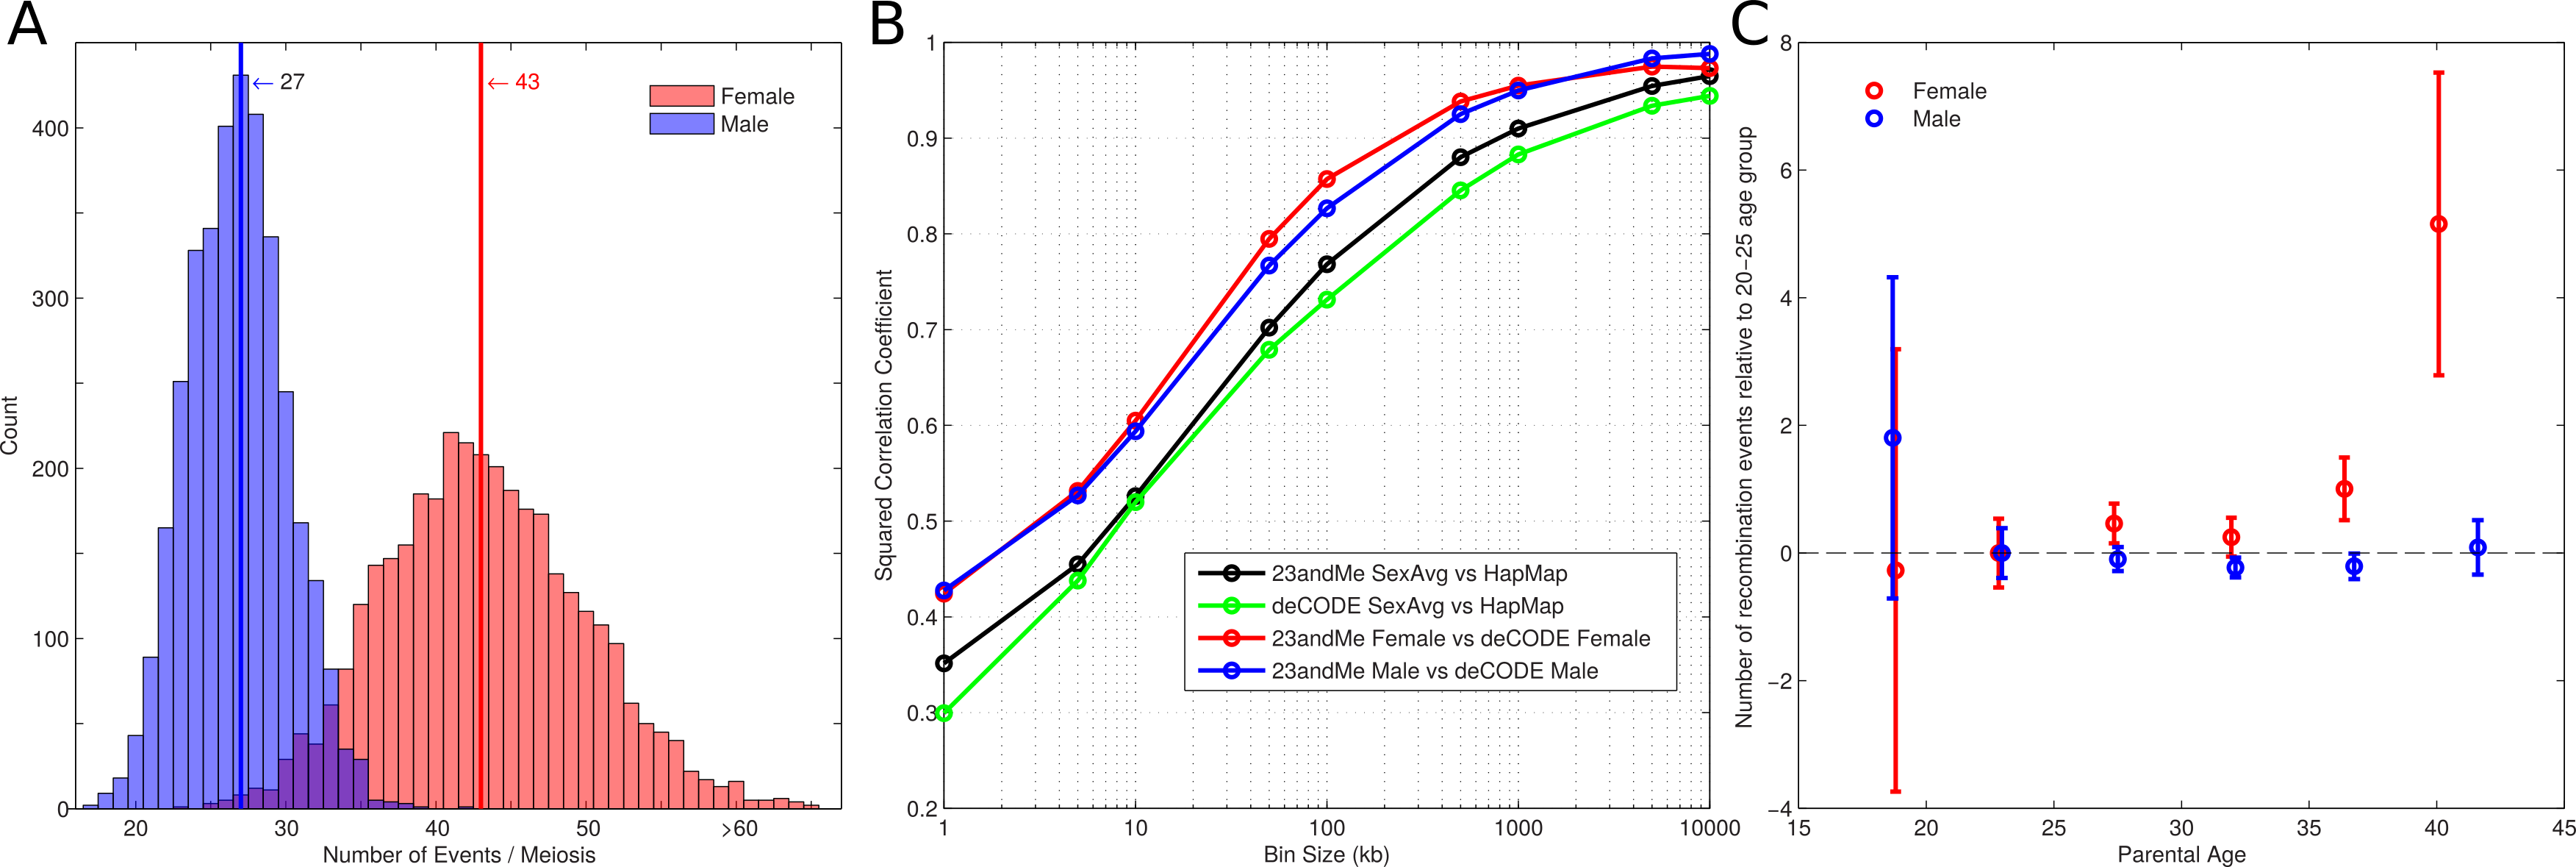
\includegraphics[width=\textwidth]{cointEscape/figs/Figure1.png}
    \vspace{-20pt}
    \captionTitle{\textbf{Properties of recombination partitioned by sex and age.}}{ 
        (a) The number of events per meiosis for females (red, n $=$ 9152) and males (blue, n $=$ 9150), with median values indicated by a vertical line. For phase-unknown individuals, the average number of events per meiosis was used. 
        (b) Squared Pearson correlation between the 23andMe map, the deCODE map and the HapMap map, as a function of scale. 
        (c) The number of recombination events as a function of parental age for females (red, n $=$ 9152) and males (blue, n $=$ 9150), relative to parents of between 20 and 25 years of age. Parents were grouped into 5-year age bins, and the mean number of events estimated. Error bars show a 95\% confidence interval for each group.
    \label{fig:cointF1}}
\end{figure}

Treating the overall recombination rate as a phenotype, we
replicate genetic associations at genome-wide significance for
RNF212, which is known to be essential for crossover-specific
complexes\cite{Reynolds2013}, and within the vicinity of TTC5, which appears
to replicate an association with CCNB1IP1 (\citet{Kong2014}). Another
association near SMEK1 also replicates discoveries elsewhere\cite{Kong2014},
but not at genome-wide significance (Supplementary Table 4).

Previous reports have suggested increased recombination rates
in older females\cite{Kong2004,Coop2008}. Using linear regression (Supplementary
Fig. \ref{fig:cointFS6}), we obtain a similar result with an additional 0.067
events per year being observed in females ($P=$ 0.002, F-test), and
no such effect being observed in males ($P=$ 0.30, F-test). The
female effect appears to be driven by sharp increase in the
number of recombination events for older mothers (Fig. \ref{fig:cointF1}c).
Fitting the piecewise-linear model with a single change point
infers a rapid increase in the female recombination rate after 38.8
years, increasing from 0.047 events per year to 2.990 events per
year. On average, mothers of 39 years and over have an additional
2.51 events compared with younger mothers ($P=$ 0.0005,
Mann-Whitney U).

One possible interpretation of the increasing number of
recombination events with maternal age is that mothers with
higher recombination rates can maintain fertility until a later
age\cite{Kong2004} . To investigate this possibility, we focused on 776 mothers
(providing 2,184 meioses) that were part of larger families and
could have recombination events assigned to specific children.
After subtracting off the average age and average number of
recombination events for each mother, the resulting regression
does not find a significant association with age ($P=$ 0.11, F-test),
although we estimate our power to detect an effect size of an
additional 0.067 events per year in this subsample to be no more
than 30\%.

Both pedigree and LD studies have suggested that $\sim$60-70\% of
crossover events occur within recombination hotspots\cite{Coop2008,Myers2005}. Our
data confirm this result with 62.7\% of events occurring within
LD-defined hotspots in females, and 67.3\% occurring within
hotspots in males (Fig. \ref{fig:cointF2}a; Supplementary Fig. \ref{fig:cointFS7}A). The 4.6\%
difference between the two sexes is highly significant
($P=$ \num{1.1e-69}, Mann-Whitney U), suggesting differences in
the regulation of crossover placement between the sexes. The
result remains significant after thinning the female data to match
the crossover density of the male data ($P<$ \num{2.2e-16},
Mann-Whitney U), and does not appear to be driven by
increased male recombination rates near the telomeres (see
Supplementary Methods).

Hotspot localization is believed to be under the control of the
zinc-finger protein PRDM9, which recognizes and binds specific
DNA motifs\cite{Berg2010,Berg2011,Hinch2011,Parvanov2010}. We find single-nucleotide polymorphisms
(SNPs) in the vicinity of PRDM9 to be strongly associated with
the degree of hotspot usage, as has previously been reported\cite{Kong2014,Hinch2011}.
The most strongly associated SNP is rs73742307 achieving a
P value of \num{7.9e-184} (\citet{Reynolds2013}), with no other region achieving a
genome-wide significant association with this phenotype
(Supplementary Table 5).

Variation within the PRDM9 DNA-binding domain can result
in changes to the recognized motif and hence lead to differences
in hotspot localization between individuals. While the major allele
of PRDM9 (allele A) is present at high frequency in most human
populations, a large number of low-frequency alleles have been
observed, particularly within African populations\cite{Berg2011,Parvanov2010}. Consistent
with this, we find hotspot usage to be significantly lower within
individuals of African ancestry (Fig. \ref{fig:cointF2}b; Supplementary Table \ref{tab:cointTS6}),
which reflects the fact that the LD-defined hotspots are expected
to mostly represent the common PRDM9 allele. Notably, while
over 75\% of our data are derived from individuals of European
ancestry, hotspot usage is higher for males than females across all
ancestries.

\begin{figure}[h]
    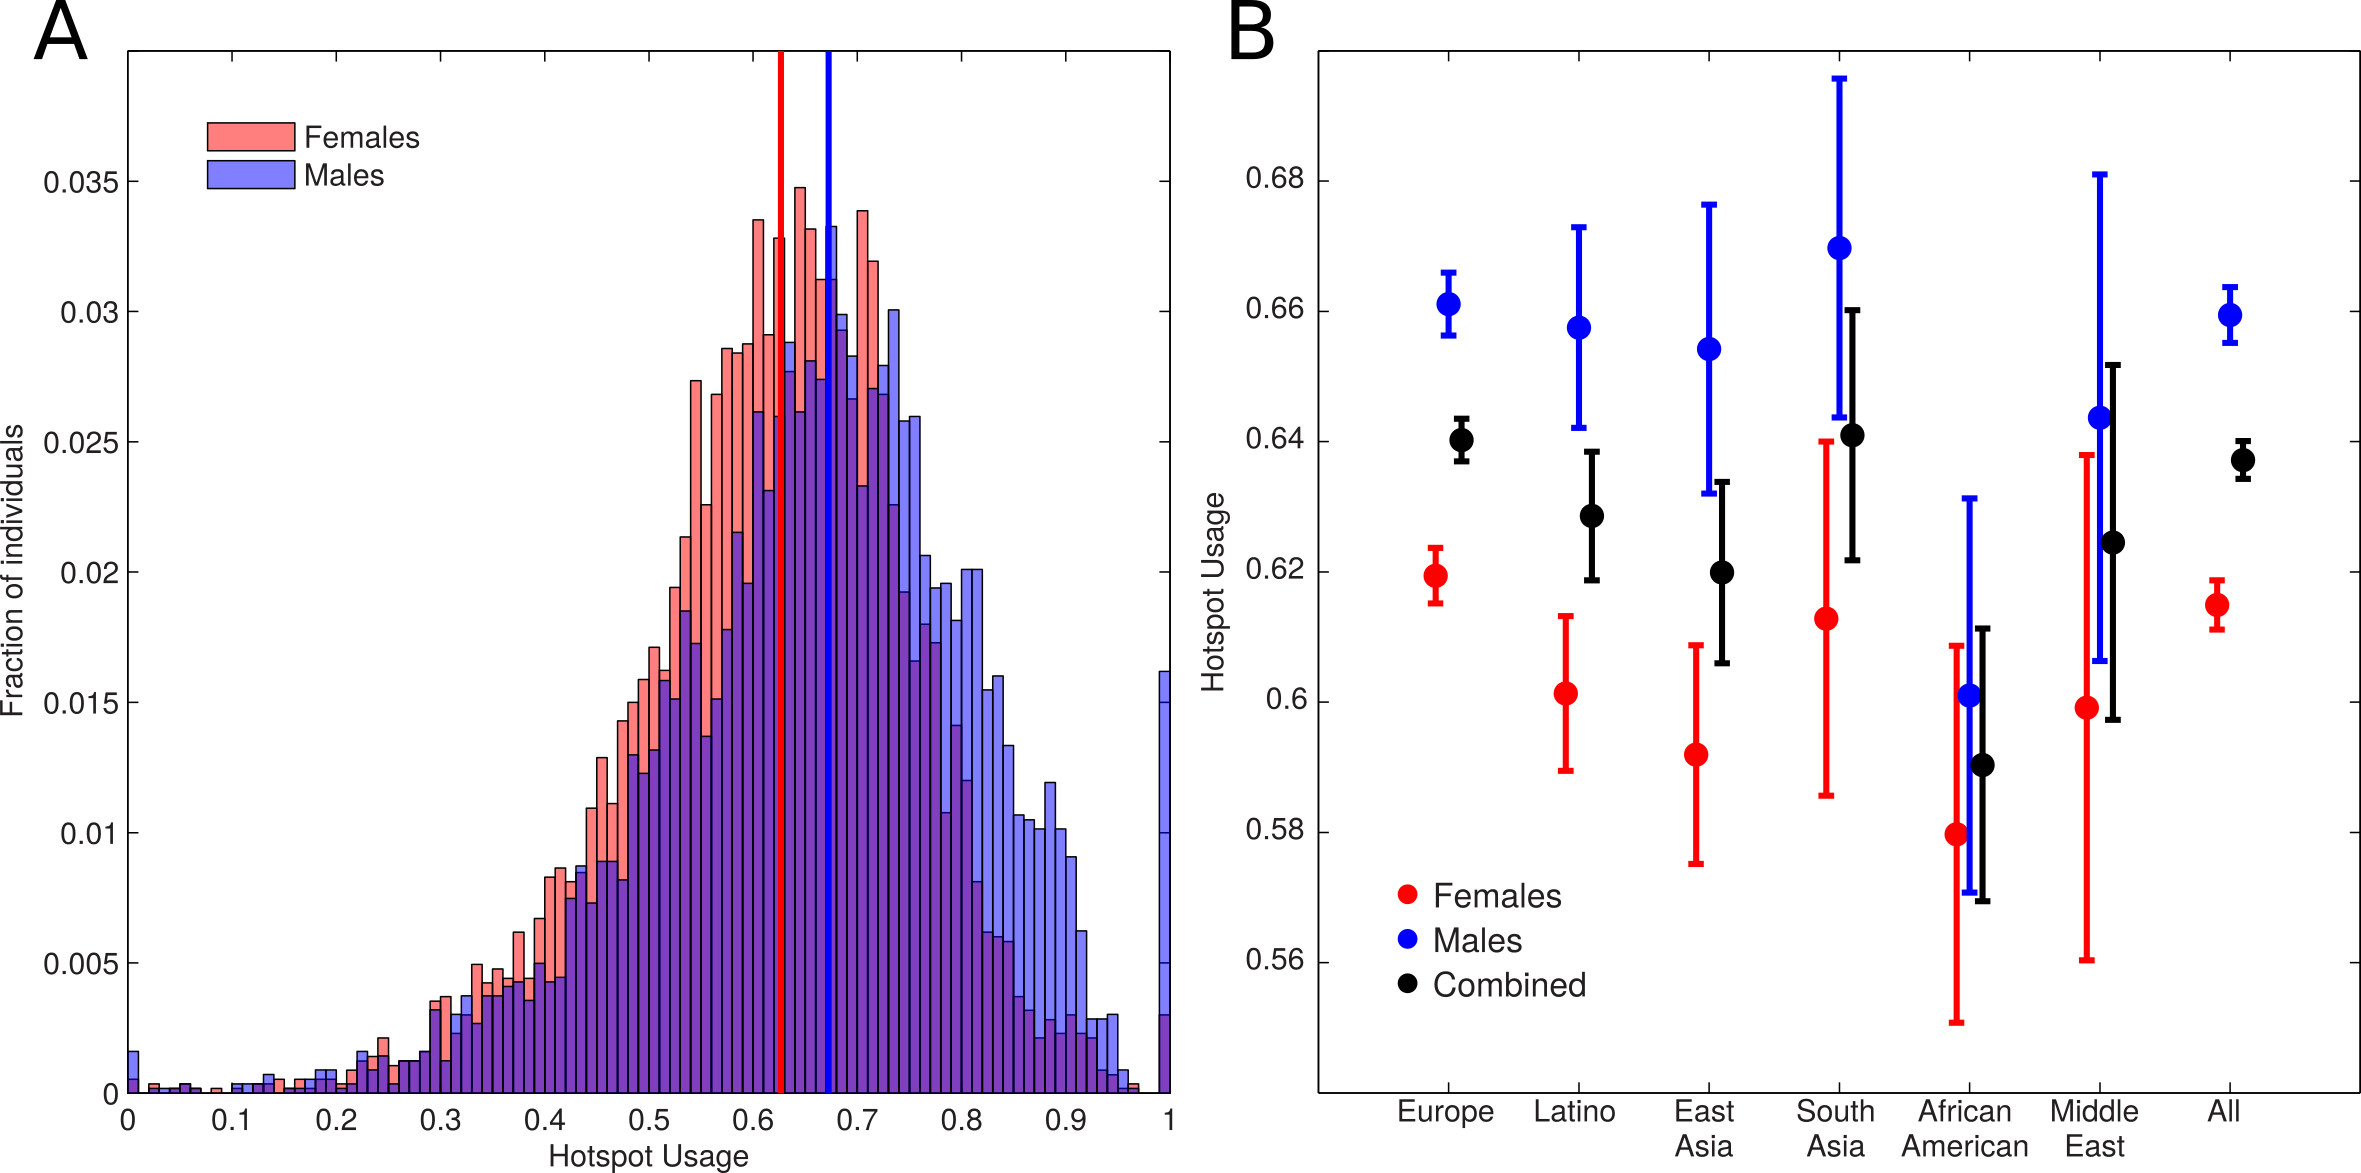
\includegraphics[width=\textwidth]{cointEscape/figs/Figure2.png}
    \vspace{-20pt}
    \captionTitle{\textbf{Sex differences in recombination hotspot usage.}}{
        (a) Hotspot usage for female (red, n $=$ 9152) and male (blue, n $=$ 9150) meioses. Median values for each sex are shown by vertical lines. 
        (b) Mean hotspot usage, subdivided by parental population. Females are shown in red, males in blue and a combined estimate in black. Error bars indicate a 95\% confidence interval.
       \label{fig:cointF2}}
\end{figure}

We find a weak association between hotspot usage and
maternal age (Supplementary Fig. \ref{fig:cointFS7}B). Using logistic regression,
we estimate a decrease in hotspot usage corresponding to
$\sim$1\% over a 10-year period ($\beta_1=$ \num{-0.0042}, $\text{s.e.}=$ \num{9.6e-4}, 
$P=$ \num{1.2e-5}, F-test). To ensure this effect is not driven by
differences in parental ancestry within the sample, we repeated
the analysis only using individuals of European ancestry. In this
case, the effect size remains similar ($\beta_1=$ \num{-0.0033}, $\text{s.e.}=$ 0.0013),
but is only marginally significant ($P=$ 0.0101, F-test). Including
the number of events as an additional predictor variable within
the regression leaves age as a weakly significant predictor
($P=$ 0.0106, F-test), but not the number of events ($P=$ 0.74,
F-test). Despite the small size of the estimated effect, we note that
no such age-related effects were observed in males.

To learn more about interactions between recombination
events, we used the high number of crossover locations in our
data to better characterize the phenomenon of crossover
interference. By considering the distribution inter-crossover
distances, we fit three models to describe the distribution of
inter-crossover distances: a model without interference between
crossovers (also known as the gamma model of crossover
interference\cite{Broman2000}), and a mixture model in which a subset of
events come from a process that exhibits no interference (also
known as the Housworth-Stahl model\cite{Housworth2003}). To fit these models, we
used existing methods for families in which recombination events
could be assigned to specific individuals, and extended these
methods for smaller families where recombination events cannot
be simply assigned to a specific individual (see Supplementary
Methods).

In agreement with previous reports\cite{Housworth2003,Fledel-Alon2009}, the Housworth-Stahl
interference escape model provides a much better fit to our
data than either the gamma simple interference model or the
interference-free model (Fig. \ref{fig:cointF3}a). Under this model, the estimates
of the strength of crossover interference are similar to previous
reported using smaller data sets\cite{Fledel-Alon2009}. The degree of interference is
inferred to be lower in females than in males ($\nu_{female}=$ 7.19 vs
$\nu{male}=$ 8.93). In addition, 7.8\%/6.7\% of female/male events are
inferred to escape interference. We therefore conclude that a
non-negligible fraction of crossovers occur in the absence of
crossover interference.

We find evidence that both the degree of interference and
interference escape varies across chromosomes (Fig. \ref{fig:cointF3}b,c;
Supplementary Table \ref{tab:cointTS7}). The strength of interference is reasonably 
well predicted by the chromosome map length ($r^2=$ 0.565,
$P=$ \num{6.4e-9}), although the relationship is only significant in
females when considering the sexes separately ($r^2_{female}=$ 0.69,
$P=$ \num{1.7e-6} and $r^2_{male}=$ 0.172, $P=$ 0.06; Supplementary Fig. \ref{fig:cointFS8}).
In contrast, the fraction of events escaping interference shows no
relationship with chromosome map length ($r^2=$ 0.001, $P=$ 0.84).
Certain chromosomes appear to have high degrees of escape, with
chromosomes 8, 9 and 16 (in females) being notable outliers.

\begin{figure}[h]
    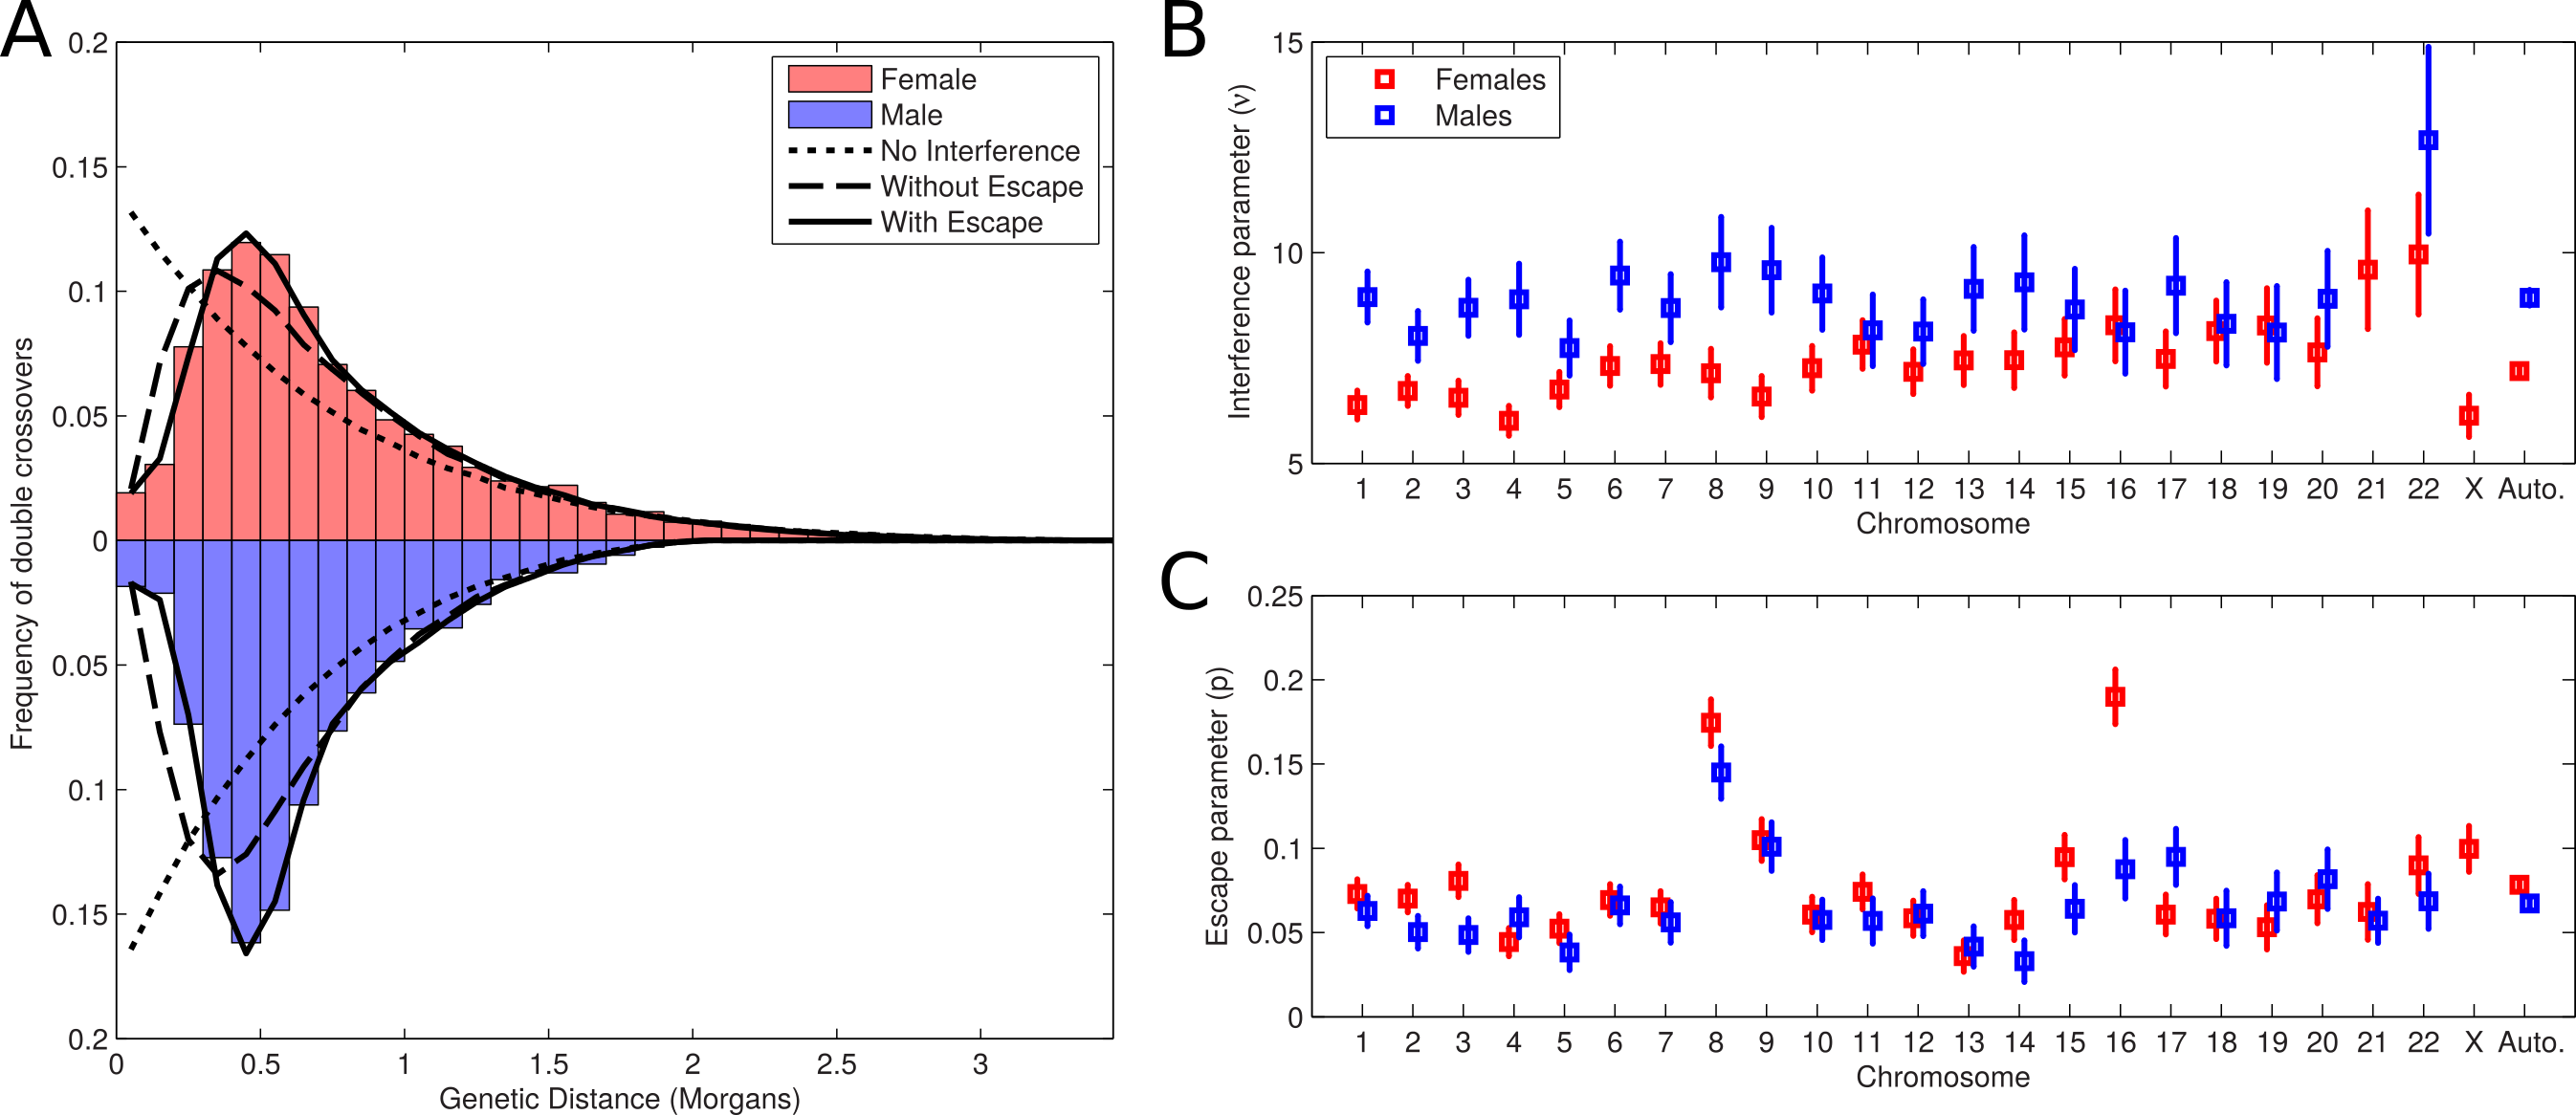
\includegraphics[width=\textwidth]{cointEscape/figs/Figure3.png}
    \vspace{-20pt}
    \captionTitle{\textbf{Estimation of crossover interference parameters.}}{
        (a) Fit of three models of interference to the inter-crossover distances observed on chromosome 1, derived from phase-known mothers (red, n $=$ 2184) and fathers (blue, n $=$ 2092).
        The interference-free model is shown as a dotted line, the gamma simple interference model is shown as a dashed line and the Housworth-Stahl interference escape model is shown as a solid line. 
        (b) Per-chromosome estimates of the interference parameter as estimated from the Housworth-Stahl interference escape model.
        Error bars indicate a 95\% confidence interval.
        Note that chr21 in males is excluded due to an extremely high estimate.
        (c) Per-chromosome estimates of the proportion of events escaping interference. Error bars indicate a 95\% confidence interval.
       \label{fig:cointF3}}
\end{figure}

To investigate whether crossover interference changes with
parental age, we subdivided our data into 10 quantiles on the
basis of age, and fit the Housworth-Stahl interference escape
model to each group independently. We observe a striking
increase in the proportion of events that escape interference with
maternal age (Fig. \ref{fig:cointF4}a), rising from 6.7\% for mothers under 25
years to 9.5\% for mothers over 35 years. No such correlation is
observed for the interference parameter in females, and no
correlation is observed for either parameter in males
(Supplementary Fig. \ref{fig:cointFS9}). The effect is robust to different subdivisions % edited typo
of the data (Supplementary Figs \ref{fig:cointFS10} and \ref{fig:cointFS11}).

A potential concern is that the detected increase in interference
escape could be driven by the observed increased number of
crossovers in older mothers. If the number of crossovers is 
increased, then the distances between them are necessarily
shorter, which may in turn influence the interference parameter
estimates. To account for this possibility, we performed stratified
sampling of individuals to control for the number of events
within each quantile. The observed increase in the escape
parameter with maternal age is still observed (Supplementary
Fig. \ref{fig:cointFS12}), indicating that it is not driven by changes in the overall
recombination rate.

To further investigate the differences between old and young
parents, we plotted the distribution of inter-crossover distances
for young and old parents (Fig. \ref{fig:cointF4}b,c). The interference escape
effect in females appears to be predominately driven by an
increase in the number of very tightly clustered events, generally
separated by less than $\sim$5 cM. These tightly clustered events are
not well captured by the Housworth-Stahl interference escape
model (Supplementary Fig. \ref{fig:cointFS13}), and a major concern therefore is
that these tightly clustered events represent false-positive calls
arising from genotyping error. However, the effect remains even
if we apply much stricter filtering of the crossover events
(Supplementary Fig. \ref{fig:cointFS14}), and in addition we believe genotyping
error is unlikely to explain the association between the escape
parameter and maternal age because (a) the effect is not seen in
males, and (b) it would imply increased genotyping error for
older mothers (but not fathers).

\begin{figure}[h]
    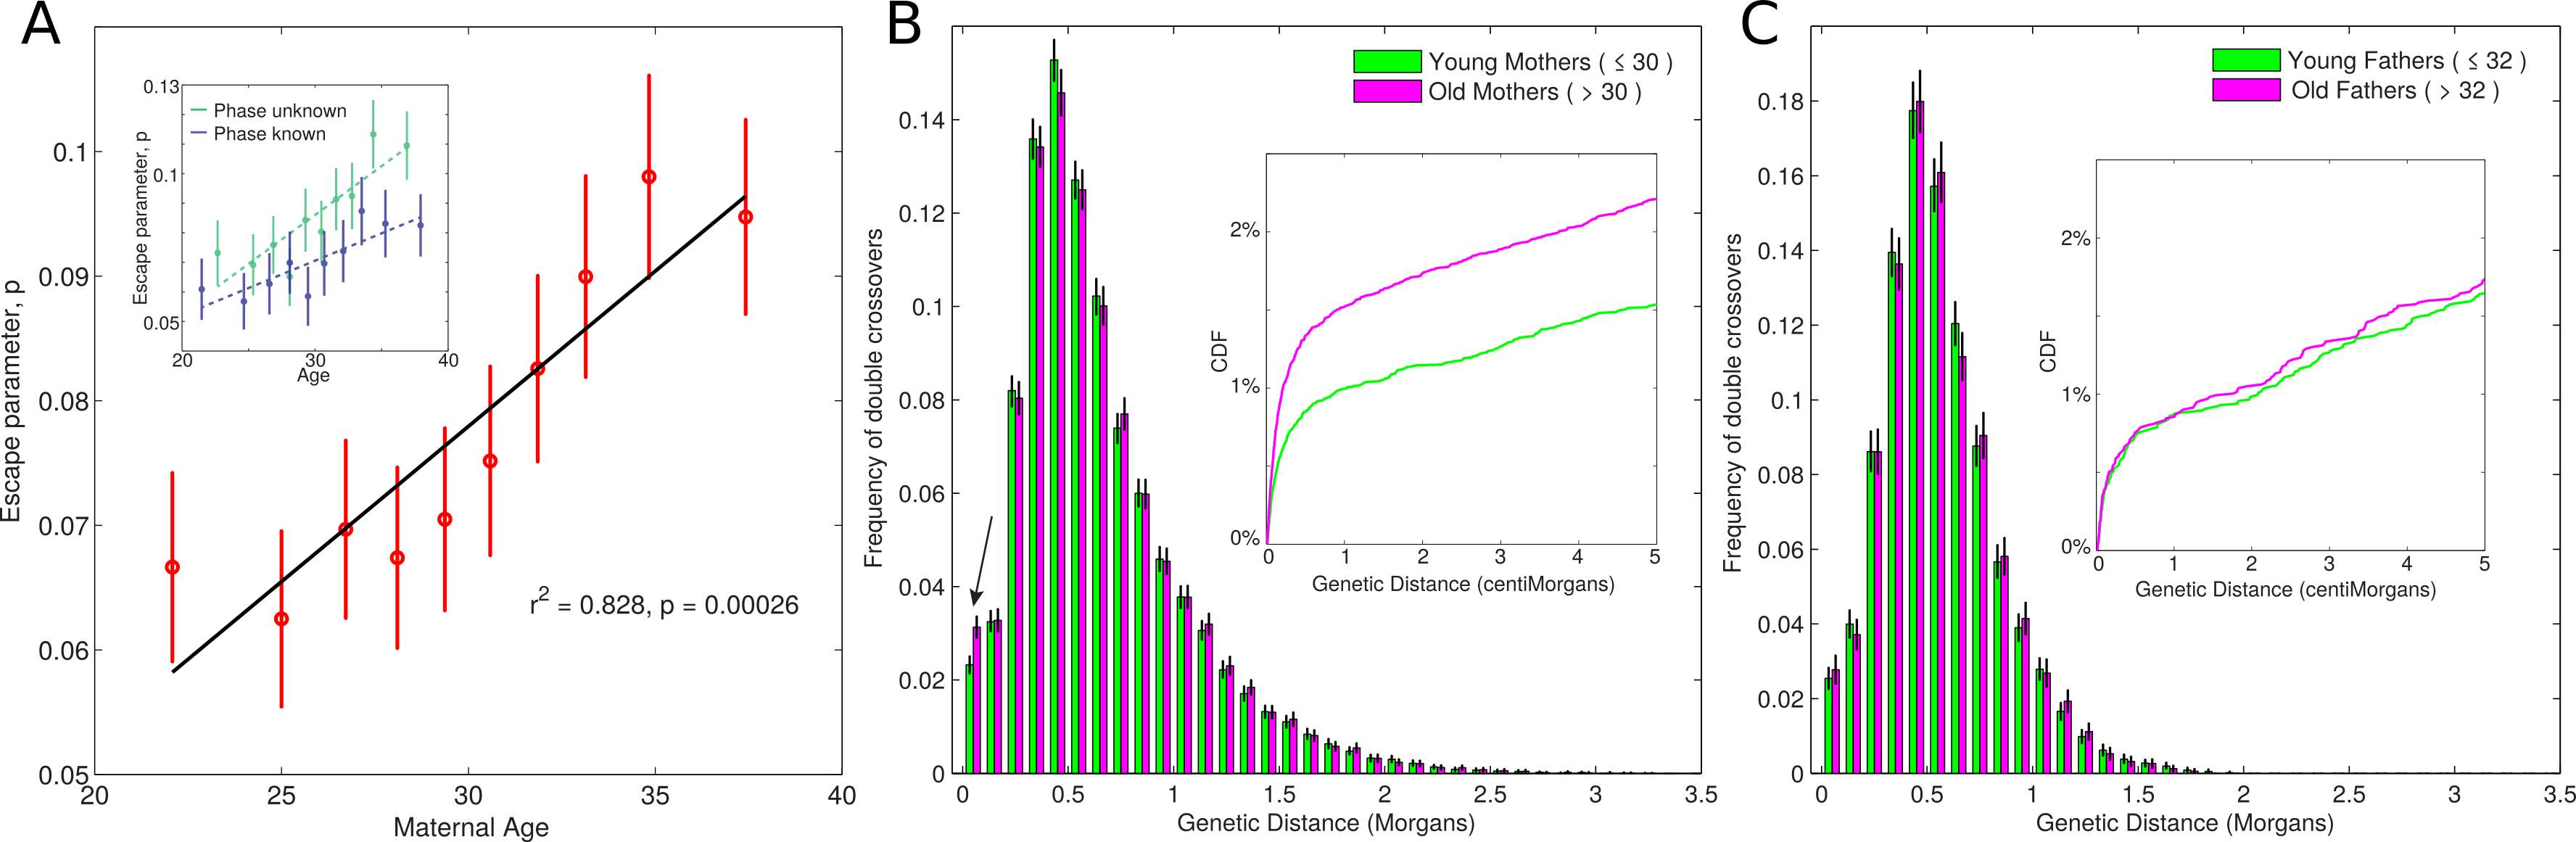
\includegraphics[width=\textwidth]{cointEscape/figs/Figure4.png}
    \vspace{-20pt}
    \captionTitle{\textbf{Departures from simple crossover interference.}}{
        (a) Inferred escape parameter as a function of maternal age.
        Mothers were divided into 10 approximately equal-sized deciles on the basis of age, and the Housworth-Stahl interference escape model was fitted for each group separately.
        The inset shows the estimates of the escape parameter when considering phase-known (blue, n $=$ 2184) and phase-unknown (green, n $=$ 6968) individuals separately. 
        Estimates for $\nu$ show no correlation with age (Supplementary Fig. \ref{fig:cointFS9}). Error bars indicate 95\% confidence intervals. 
        (b) Distribution of inter-crossover distances for young and old mothers, where the boundary between young and old is taken as median maternal age (30 years). 
        Error bars represent a 95\% confidence interval assessed via 1000 bootstrap samples, and the arrow highlights a significant difference between the young and old groups for tightly clustered events. 
        The inset shows the cumulative distribution function (CDF) up to 5 cM. 
        (c) Distribution of inter-crossover distances for young and old fathers, where the boundary between young and old is taken as median paternal age (32 years).
       \label{fig:cointF4}}
\end{figure}

In terms of meiosis, a major difference between the sexes is that
female meiosis starts during fetal development, but does not
complete until adulthood. As such, while male gametes are
produced throughout adulthood and promptly proceed through
meiosis, oocytes remain arrested in a late stage of prophase
(dictyotene) for many years, if not decades. Presuming our
observation of increasing crossover interference escape with
maternal age is not due to some obscure form of genotyping
error, our observations add to similar evidence of increasing rates
of recombination\cite{Kong2004} and aneuploidy\cite{Hassold2001} in aging females. Although
these phenomena are presumably related, the biological
mechanisms by which they occur are unclear, and we can think
of at least three possibilities. First, given chromatids remain
physically proximal during the extended period of female meiotic
arrest, one possible explanation is that additional recombinations
are initiated during this time, perhaps in response to
DNA damage. However, as recombination is believed to have
completed by the time of dictyotene, such an explanation appears
unlikely. A second possibility, previously invoked to explain the
increasing recombination rate with maternal age\cite{Kong2004}, suggests
oocytes with additional recombination events could be at
reduced risk of nondisjunction, and hence would be more likely
to lead to viable embryos in older mothers. However, it is not
clear that this mechanism would explain the increased clustering
of events observed in our data. Finally, a third possibility is 
related to the so-called ``production line'' hypothesis, in which
oocytes are selected for maturation sequentially in the same order
as their generation, and later oocytes have therefore potentially
undergone additional mitotic divisions prior to entering
meiosis\cite{Reizel2012}. However, the existence of a production line has been
debated for many years\cite{Reizel2012,Polani1991,Rowsey2014}, and so the likelihood of this
explanation is unclear.

%%%%%%%%%%%%%%%%%%%%%%%%%%%%%%%%%%%%%%%%
%%%%%%%%%%%%%%%%%%%%%%%%%%%%%%%%%%%%%%%%
\section{Methods}
%%%%%%%%%%%%%%%%%%%%%%%%%%%%%%%%%%%%%%%%
%%%%%%%%%%%%%%%%%%%%%%%%%%%%%%%%%%%%%%%%

\paragraph{Sample genotyping.} Samples were collected and genotyped at the consumer
genetics company 23andMe Inc., as described previously\cite{Eriksson2010}. Briefly, genotyping was
performed on genomic DNA extracted from saliva samples. DNA was genotyped
on one of two microarray platforms: the Illumina HumanHap550+ BeadChip
platform, which includes more than 550,000 SNPs, or the Illumina
HumanOmniExpress+ BeadChip, which has a base set of 730,000 SNPs
augmented with $\sim$250,000 SNPs to obtain a superset of the HumanHap550+,
as well as a custom set of about 30,000 SNPs.

\paragraph{Pedigree construction.} Pedigrees were constructed first by identifying trios using
estimated identity-by-decent relationships. Trios were then combined to form
nuclear families, and nuclear families were joined based on the assumed
relationships to form larger pedigrees. We identified trios by finding triplets of
individuals in the 23andMe customer cohort that had estimated identity-by-decent
relationships matching those expected in a true trio. Trios were accepted if both
parents were at least 18 years old upon the birth of the child and one parent was
male and the other female. We created nuclear families by identifying all trios with
the same two parents and then by combining the children of these trios. Finally,
larger pedigrees were created by simply joining the nuclear families based on the
assumed relationships and by accounting for directionality given by the age of
individuals. Any two individuals with more than one potential relationship were
excluded along with the pedigrees they belonged to.

\paragraph{Calling of recombination events and data filtering.} Prior to data filtering,
the data set consisted of 4,270 pedigree families, with data pertaining to 18,647
informative meioses. This raw data set consisted of 692,876 recombination events,
with a median of 45 and 28 events per meiosis in females and males, respectively.

The Merlin algorithm (version 1.1.2) used to detect recombination events does
not account for genotyping error, and genotyping errors are therefore likely to
result in spurious recombination event calls. To account for this issue, our first step
was to only use high-confidence sites. First, we required the sites to have a call rate
greater than 90\% and Hardy-Weinberg $P$ value $\le$ \num{1e-20} (as calculated in the
23andMe cohort). Second, we excluded sites with minor allele frequencies differing
from those of the 1000 Genomes Phase 1 reference panel\cite{1000G2012}. This was achieved by
constructing a 2 $\times$ 2 contingency table and comparing the 1000 Genomes
European allele counts with those from 2,000 randomly selection 23andMe
customers, and using a $\chi^2$-test to identify significant deviations. Sites with $P$ values
less than \num{1e-15} were removed.

Having applied these basic site filters, we next aimed to remove any weakly
supported recombination events. This was achieved by first using the Merlin ``error''
feature to remove potential genotyping errors not consistent with gene flow within
each pedigree. In addition, we excluded all recombination events supported by less
than three recombination-informative sites on either side, where we define an
informative site as a site that is called as heterozygotic in exactly two individuals
out of each mother-father-child trio. Finally, we removed all pairs of events within
each single family that occurred within the same SNP interval. Together, these
filters removed 31,742 weakly supported events, which corresponded to 4.6\% of the
total number.

Preliminary inspection of the genetic maps identified a region on chromosome
10 where the 23andMe genetic map diverged substantially from that generated by
deCODE\cite{Kong2010}. This can be seen in a plot of the chromosome 10 genetic map at
$\sim$50 Mb (Supplementary Fig. \ref{fig:cointFS2}A).

Further investigation of this region revealed a large number of ``double''
crossovers in close proximity to each other (that is, pairs of recombination events
occurring in close proximity within the same individual). While some such
observations are expected through the action of gene conversion, such strong
clustering of these events is not expected biologically. Instead, we believe the result
is suggestive of misplacement of polymorphisms, mis-assembly of one or more
reference contigs in the hg19 reference genome or of more complex types of
error related to copy number polymorphism or array design. In any case, these
double-recombination events represent a form of error that needed to be
eliminated.

To better quantify this issue, we identified all pairs of recombination events
occurring within a single individual that were within 1 Mb of each other. For each
SNP in the genome, we estimated the number of these event pairs that span the
SNP (Supplementary Fig. \ref{fig:cointFS2}B).

For the vast majority of the genome, there were very few such event pairs, and
hence localized peaks likely represent data quality issues. We therefore identified all
SNPs spanned by at least 14 event pairs (with this threshold being equivalent 
to the 99.9th percentile of the distribution). In this way, we identified 50 regions
with strong enrichment of nearby event pairs (Supplementary Table 8). Note that
for this analysis we ignored the pseudoautosome, as a large number of events
occurring in close proximity might be expected due to the extreme male
recombination rate within this region.

The regions with high numbers of clustered events were themselves clustered
into 13 regions across 8 chromosomes, and are often in the vicinity of chromosome
centromeres, telomeres or reference assembly gaps. We removed all event pairs
within 500 kb of the region boundaries described in Supplementary Table 8, which
resulted in the removal of 2,916 events (0.42\% of the total). The removal of these
events improved the concordance between the 23andMe and deCODE maps
(Supplementary Fig. \ref{fig:cointFS2}C).

Previous research using well-curated data in 728 meioses reported an average of
39.6 autosomal events per gamete in females (95\% CI 38.5-40.6), and 26.2
autosomal events per gamete in males (95\% CI 25.6-26.7)7. The minimum/
maximum number of observed autosomal events in any given meiosis in this
data was 19/71 for females, and 16/43 for males (Graham Coop, personal
communication).

Preliminary analysis of our data revealed a small subset of individuals had
biologically unrealistic numbers of recombination events. Our first filtering step
was to remove the pedigrees containing these individuals. Specifically, we removed
individuals (and their containing pedigrees) that were more than 5 s.d. from the
(sex specific) median number of recombination events. To guard against outliers,
we used a robust estimate of the s.d. taken as $\sigma=$ 1.4826 MAD, where MAD
represents the median absolute deviation.

Before filtering, the median number of recombination events was 43 and 27 for
females and males, respectively (including chrX and the pseudoautosome). Using
the $\pm$5$\sigma$ thresholds, we removed pedigrees containing any female with fewer than
10 or more than 76 events per meiosis, or any male with fewer than 9 or more than
45 events. These filters removed a total of 52 pedigrees.

\paragraph{Summary of the filtered data set.} After applying the filtering steps described
above, the filtered data set consists of 4,209 pedigrees containing 18,302
informative meioses, of which 9,152 are from females and 9,150 are from males.
Of the families included in the study, 78.6\% are family quartets, 14.3\% are larger
one-generation families, and 7.1\% are two-generation families (Supplementary
Table 1).

Due to the structure of the pedigrees included in the study, certain
recombination events can be identified as having occurred within a specific child,
whereas others cannot. For example, in family quartets, it is generally unclear
which child has the recombinant haplotype, and we therefore refer to these events
as ``phase unknown''. Conversely, the child containing the recombinant haplotype
can generally be identified in larger pedigree families in which the parental
haplotype can be confidently phased, and we therefore refer to these events as
``phase known''.

In total, 4,276 meioses are derived from phase-known individuals, whereas
14,026 are derived from phase-unknown individuals. Of the female meioses, 2,184
are derived from phase-known mothers and 6,968 are from phase-unknown
mothers. Of the male meioses, 2,092 are derived from phase-known fathers, and
7,058 are derived from phase-unknown fathers.

Individuals were assigned to high-level population groups via comparison with
a set of reference populations (see Supplementary Methods). The majority of
individuals in the data set are of European descent, with $\sim$78\% of the meioses in
the sample occurring within a European individual (Supplementary Table 2).

The parental age distribution for the filtered data set is shown in Supplementary
Fig. \ref{fig:cointFS1}. The mean age was 30 years for females, and 32 for males.

The final filtered data set consists of 645,853 recombination events. Including
the sex chromosomes, the mean number of recombination events was 43.47 for
females ($\sigma=$ 6.64, 95\% CI 43.25-43.69), and 27.04 for males ($\sigma=$ 3.28, 95\% CI
26.94-27.16). For the autosomes alone, the mean number of recombination events
was 41.64 for females ($\sigma=$ 6.34, 95\% CI 41.43-41.85) and 26.61 for males
($\sigma=$ 3.26, 95\% CI 26.51-26.73).

The distribution of interval sizes to which crossovers could be resolved (that is,
the distance between informative markers on either side of the recombination
event) is given in Supplementary Fig. \ref{fig:cointFS3}. Crossovers could be resolved within a
median distance of 28.2 kb.

%%%%%%%%%%%%%%%%%%%%%%%%%%%%%%%%%%%%%%%%
\section{Acknowledgements}
%%%%%%%%%%%%%%%%%%%%%%%%%%%%%%%%%%%%%%%%
We would like to thank Hilary Martin and Julie Hussin for their constructive comments
regarding earlier versions of this manuscript. C.L.C. was supported by the Training
Program in Cellular and Molecular Biology and Genetics, T32 GM007491. Work by
N.A.F., N.E. and D.H. was supported by NIH award 2R44HG006981-02.

%%%%%%%%%%%%%%%%%%%%%%%%%%%%%%%%%%%%%%%%
\section{Author contributions}
%%%%%%%%%%%%%%%%%%%%%%%%%%%%%%%%%%%%%%%%
A.A., D.H. and N.E. designed the study. A.A., C.L.C. and N.A.F. conducted analysis.
A.A. and C.L.C. wrote the paper.

%%%%%%%%%%%%%%%%%%%%%%%%%%%%%%%%%%%%%%%%
\section{Additional information}
%%%%%%%%%%%%%%%%%%%%%%%%%%%%%%%%%%%%%%%%

\paragraph{Supplementary Information} accompanies this paper at \\ \url{http://www.nature.com/naturecommunications}

\paragraph{Competing Financial Interests:} N.A.F. and D.H. are current employees, and N.E. is a
former employee of 23andMe Inc., and have private equity interest. The remaining
authors declare no competing financial interests.

\paragraph{Reprints and permission} information is available online at \\
\url{http://npg.nature.com/reprintsandpermissions/}

\paragraph{How to cite this article:} Campbell, C. L. \textit{et al}. Escape from crossover interference
increases with maternal age. \textit{Nat. Commun.} 6:6260 doi: 10.1038/ncomms7260 (2015).

\bigskip \noindent
This work is licensed under a 
Creative Commons Attribution-NonCommercial-ShareAlike 4.0 International License. The images or
other third party material in this article are included in the article's Creative Commons
license, unless indicated otherwise in the credit line; if the material is not included under
the Creative Commons license, users will need to obtain permission from the license
holder to reproduce the material. To view a copy of this license, visit \\
\url{http://creativecommons.org/licenses/by-nc-sa/4.0/}

%%%%%%%%%%%%%%%%%%%%%%%%%%%%%%%%%%%%%%%%
%%%%%%%%%%%%%%%%%%%%%%%%%%%%%%%%%%%%%%%%
\bibliographystyle{ccampbell_thesis} %unsrtnat} %abbrvnat_noURL} %abbrvUnsrt_last-first} %plain,unsrt,alpha,abbrv,acm,apalike,unsrt
\bibliography{cointEscape/thesis-cointEscape}
%%%%%%%%%%%%%%%%%%%%%%%%%%%%%%%%%%%%%%%%
%%%%%%%%%%%%%%%%%%%%%%%%%%%%%%%%%%%%%%%%

%%%%%%%%%%%%%%%%%%%%%%%%%%%%%%%%%%%%%%%%
%%%%%%%%%%%%%%%%%%%%%%%%%%%%%%%%%%%%%%%%
\beginsupplement
\section{Supplementary Material}
%%%%%%%%%%%%%%%%%%%%%%%%%%%%%%%%%%%%%%%%
%%%%%%%%%%%%%%%%%%%%%%%%%%%%%%%%%%%%%%%%

\subsection{Supplementary Figures}

\begin{figure}[!h]
    %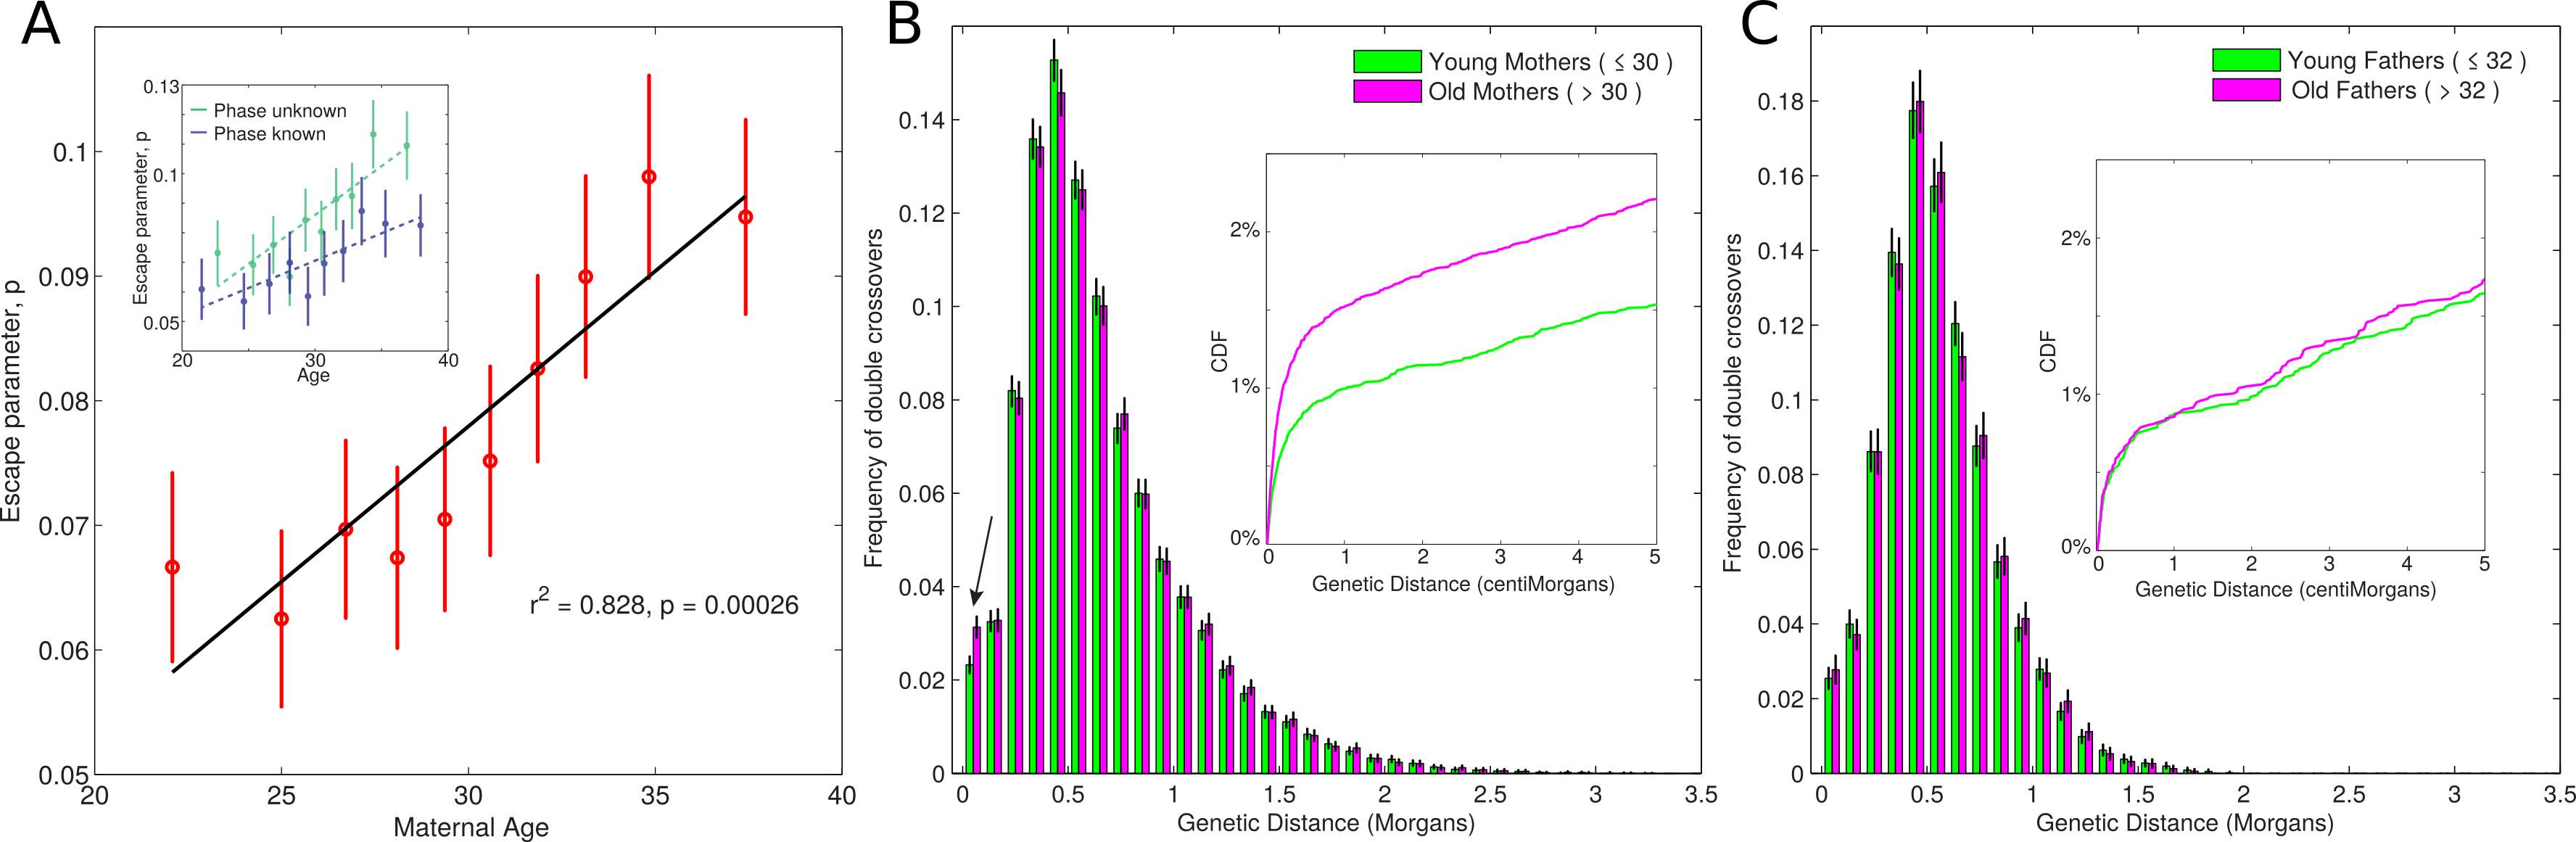
\includegraphics[width=\textwidth]{cointEscape/figs/Figure4.png}
    %\vspace{-20pt}
    \captionTitle{\textbf{Age distributions within the filtered dataset.}}{
        The left hand panel shows the distribution for phase-unknown individuals, where the parental ages were averaged across children. 
        The right hand panel shows data for the phase-known meioses where the parental age at the time of childbirth is known.
        Lines indicate the mean of each distribution. 
        Note that some families were excluded from analysis by 23andMe on the basis age to protect privacy, as seen from the truncated distribution of maternal ages in the right hand panel.  
       \label{fig:cointFS1}}
\end{figure}

\begin{figure}[!h]
    %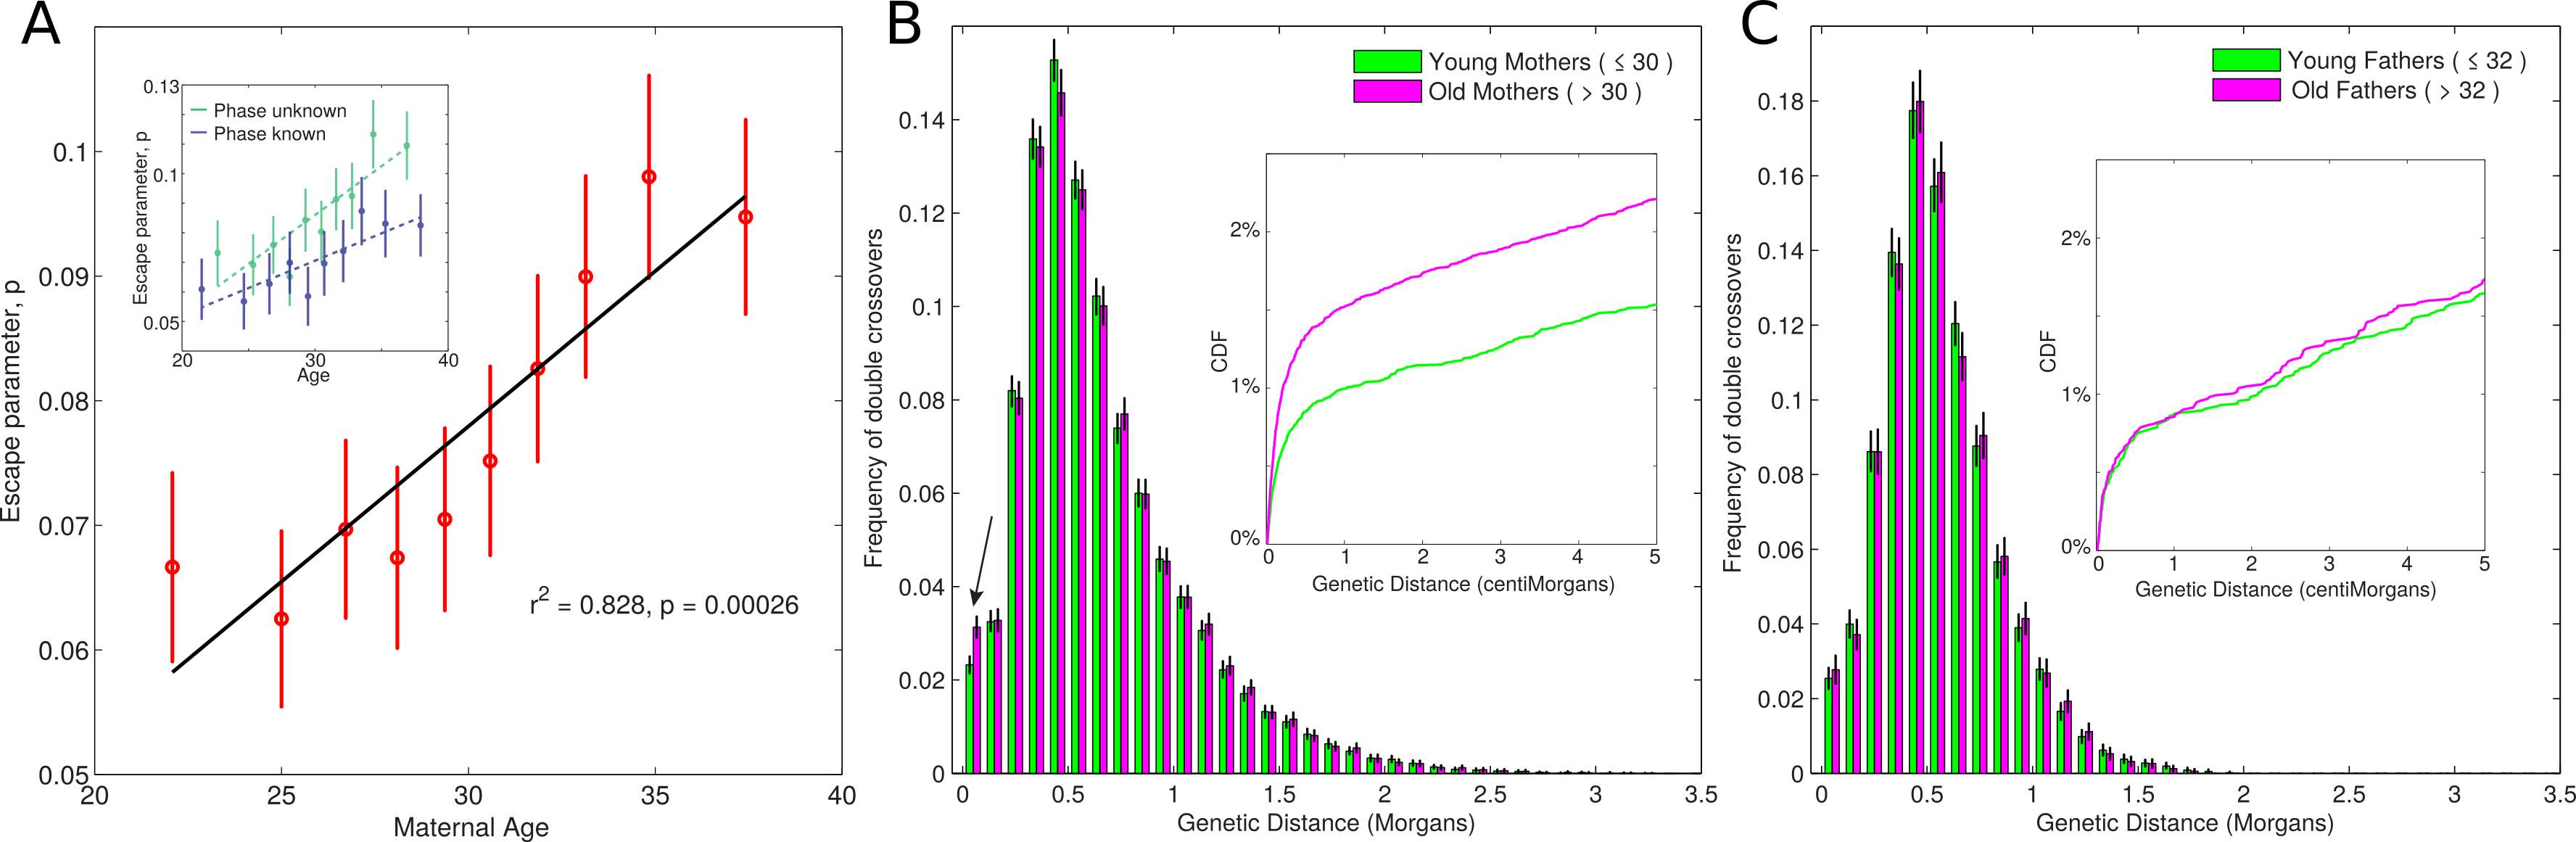
\includegraphics[width=\textwidth]{cointEscape/figs/Figure4.png}
    %\vspace{-20pt}
    \captionTitle{\textbf{Data grooming.}}{
        A) Chromosome 10 map before filtering.
        Genetic maps from the 23andMe data are shown in bold lines, whereas the genetic maps from deCODE are shown as thin lines.
        Separate maps are shown for females(red), males (blue), and sex-averaged (black). 
        Also shown are regions highlighted in grey that represent gaps in the reference assembly, the largest of which being the centromere at around 40Mb.
        B) Clustering of recombination events occurring within 1 Mb of each other within single individuals.
        Each plot shows the number of events within 1 Mb of each other on a log$_{10}$ scale as a function of physical position on each chromosome.
        A large number of these event pairs can be observed on chromosome 10, although other large peaks can also be observed on, for example, chromosomes 8 and 15.
        The dashed line represents the 99.9\% percentile of the distribution, and was used as a threshold for filtering.
        C) Chromosome 10 map after filtering.   
       \label{fig:cointFS2}}
\end{figure}

\begin{figure}[!h]
    %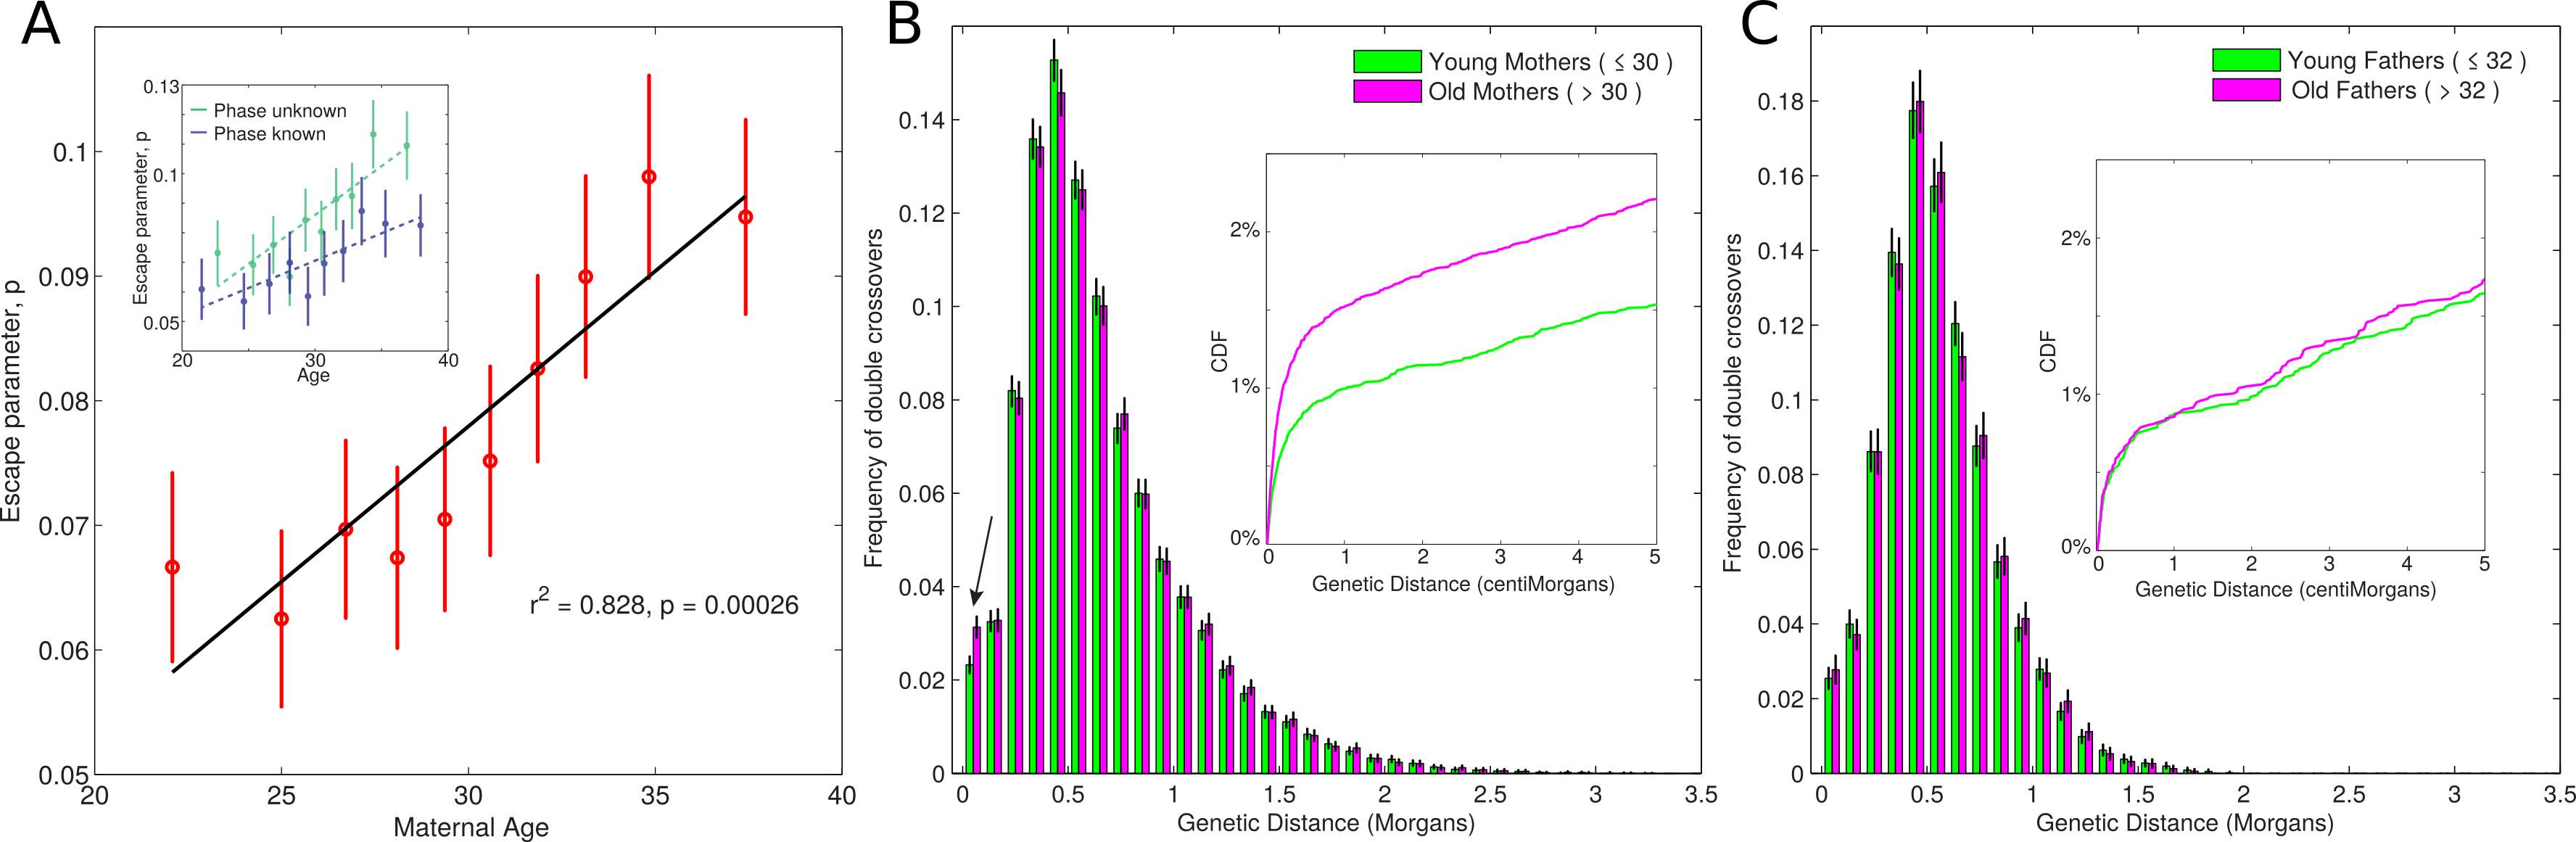
\includegraphics[width=\textwidth]{cointEscape/figs/Figure4.png}
    %\vspace{-20pt}
    \captionTitle{\textbf{Empirical cumulative distance function of crossover localization distances.}} { 
        Red labels indicate the interval distances at the distribution deciles.  
       \label{fig:cointFS3}}
\end{figure}

\begin{figure}[!h]
    %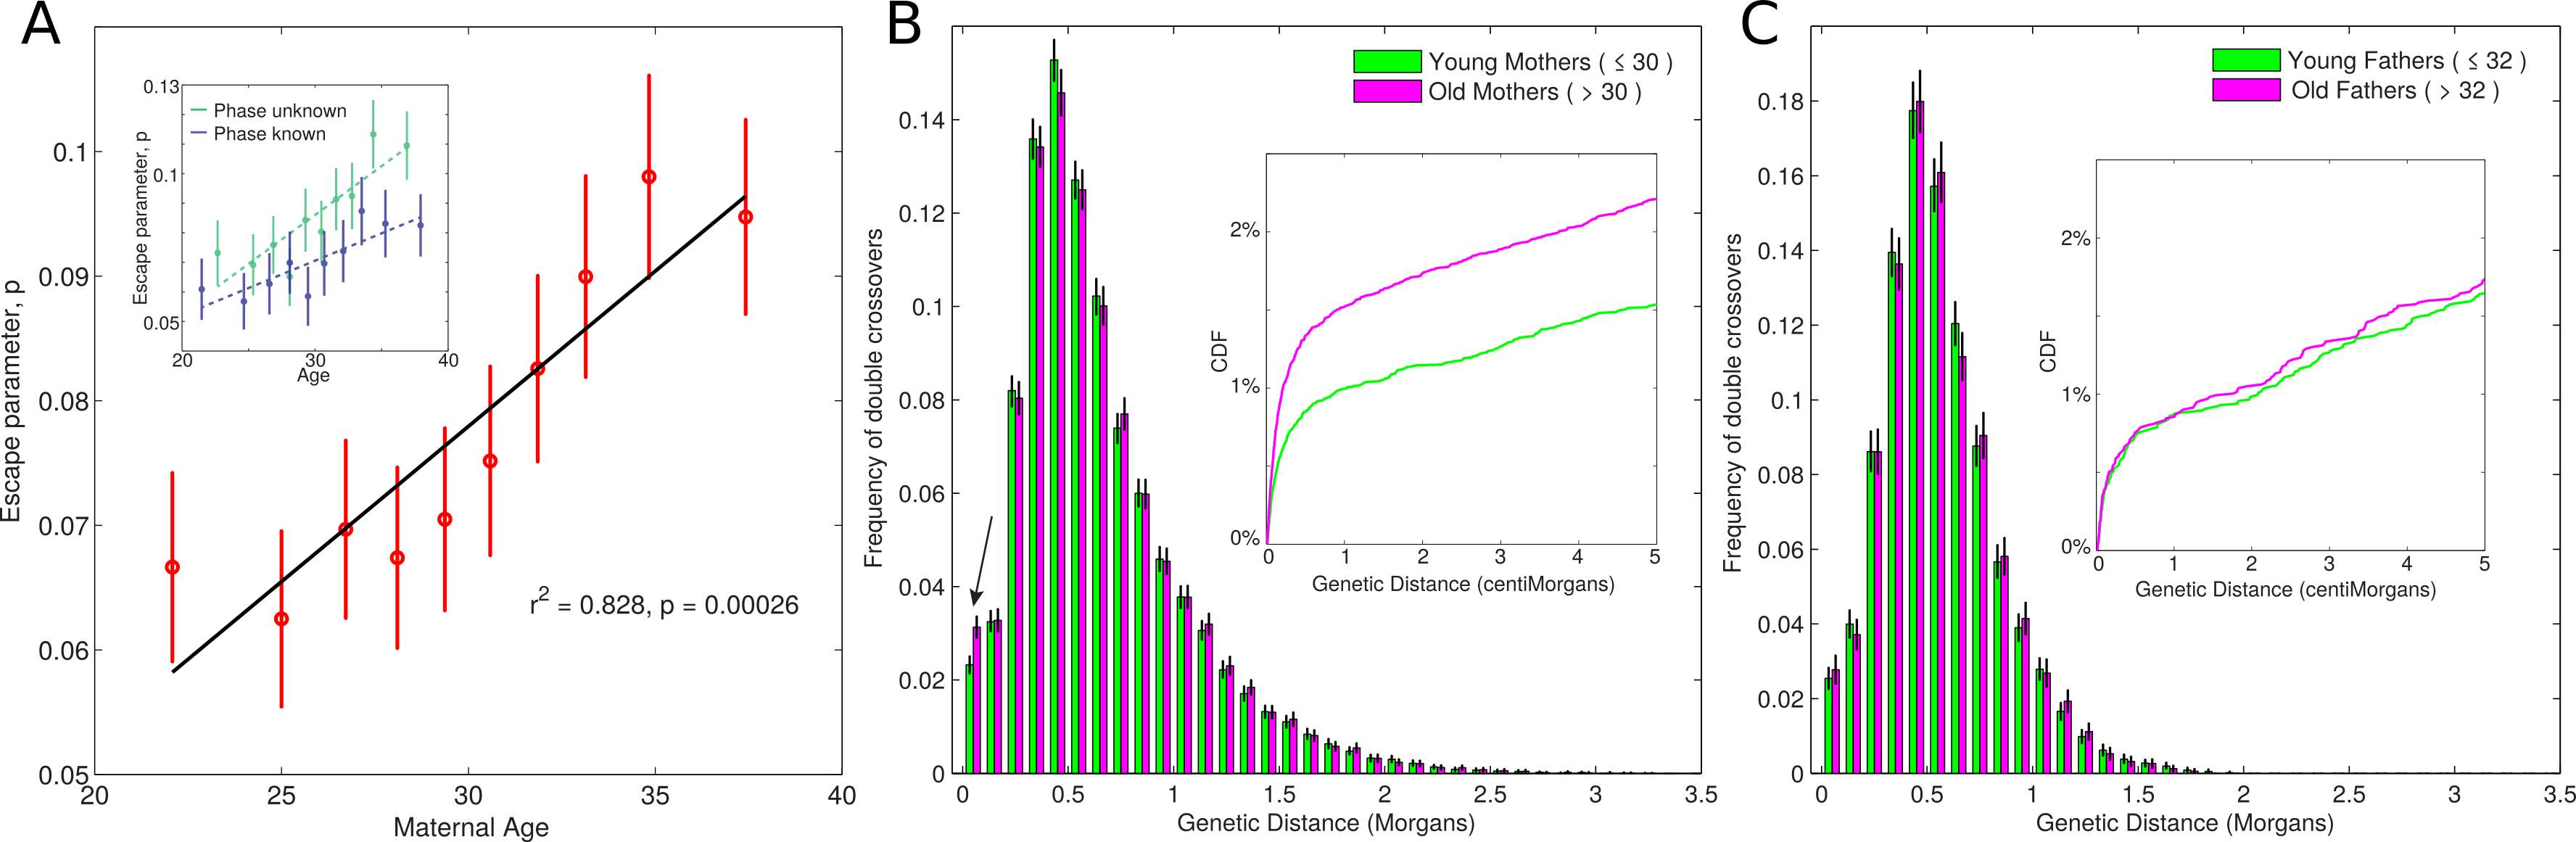
\includegraphics[width=\textwidth]{cointEscape/figs/Figure4.png}
    %\vspace{-20pt}
    \captionTitle{\textbf{Genetic map estimated from 23andMe data.}}{
        Genetic maps from the 23andMe data are shown in bold lines, whereas the genetic maps from deCODE are shown as thin lines.
        Separate maps are shown for females (red), males(blue), and sex-averaged (black).
        Also shown are regions highlighted in grey that represent gaps in the reference assembly. 
        For PAR1, we are showing data derived from Duffy\cite{Duffy2006} for comparison.
        As the deCODE maps cover a slightly smaller physical region than the 23andMe maps, the deCODE maps have been shifted slightly upwards to aid visual comparison.
        Specifically, the deCODE map has been aligned with the 23andMe map at the first physical position within the deCODE map.
        The locations of the alignments are indicated by small circles that can be most clearly seen on the smaller chromosomes.  
       \label{fig:cointFS4}}
\end{figure}

\begin{figure}[!h]
    %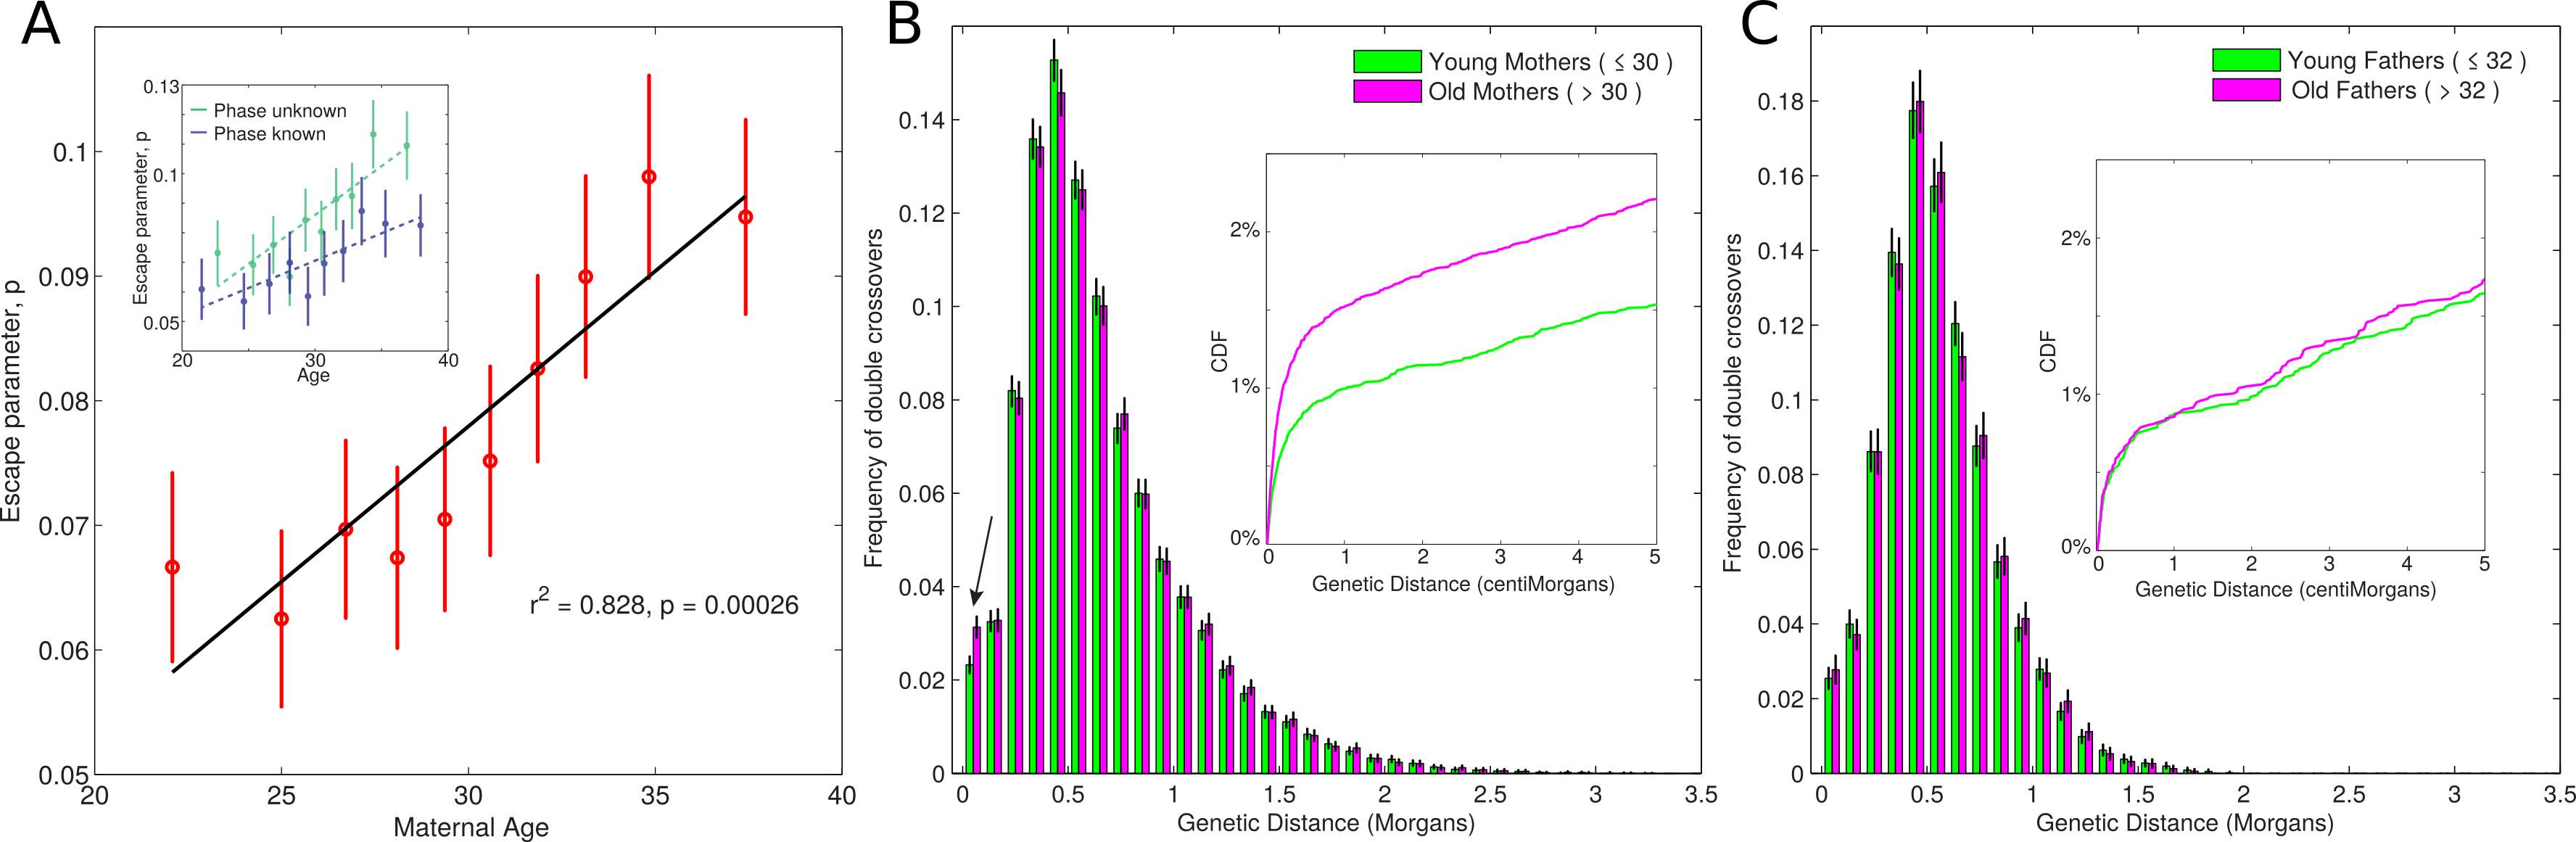
\includegraphics[width=\textwidth]{cointEscape/figs/Figure4.png}
    %\vspace{-20pt}
    \captionTitle{\textbf{The relationship between chromosome length and recombination.}}{ 
        The top row shows the correlation between physical length and map length for females (left), males (center), and sex averaged (right), with a linear fit included for the 23andMe map (red) and the deCODE map (blue).
        The bottom row shows the relationship between physical length and average recombination rate with a quadratic fit. 
        Note that chromosome X has been included in the female plots, but was excluded from the regressions.  
       \label{fig:cointFS5}}
\end{figure}

\begin{figure}[!h]
    %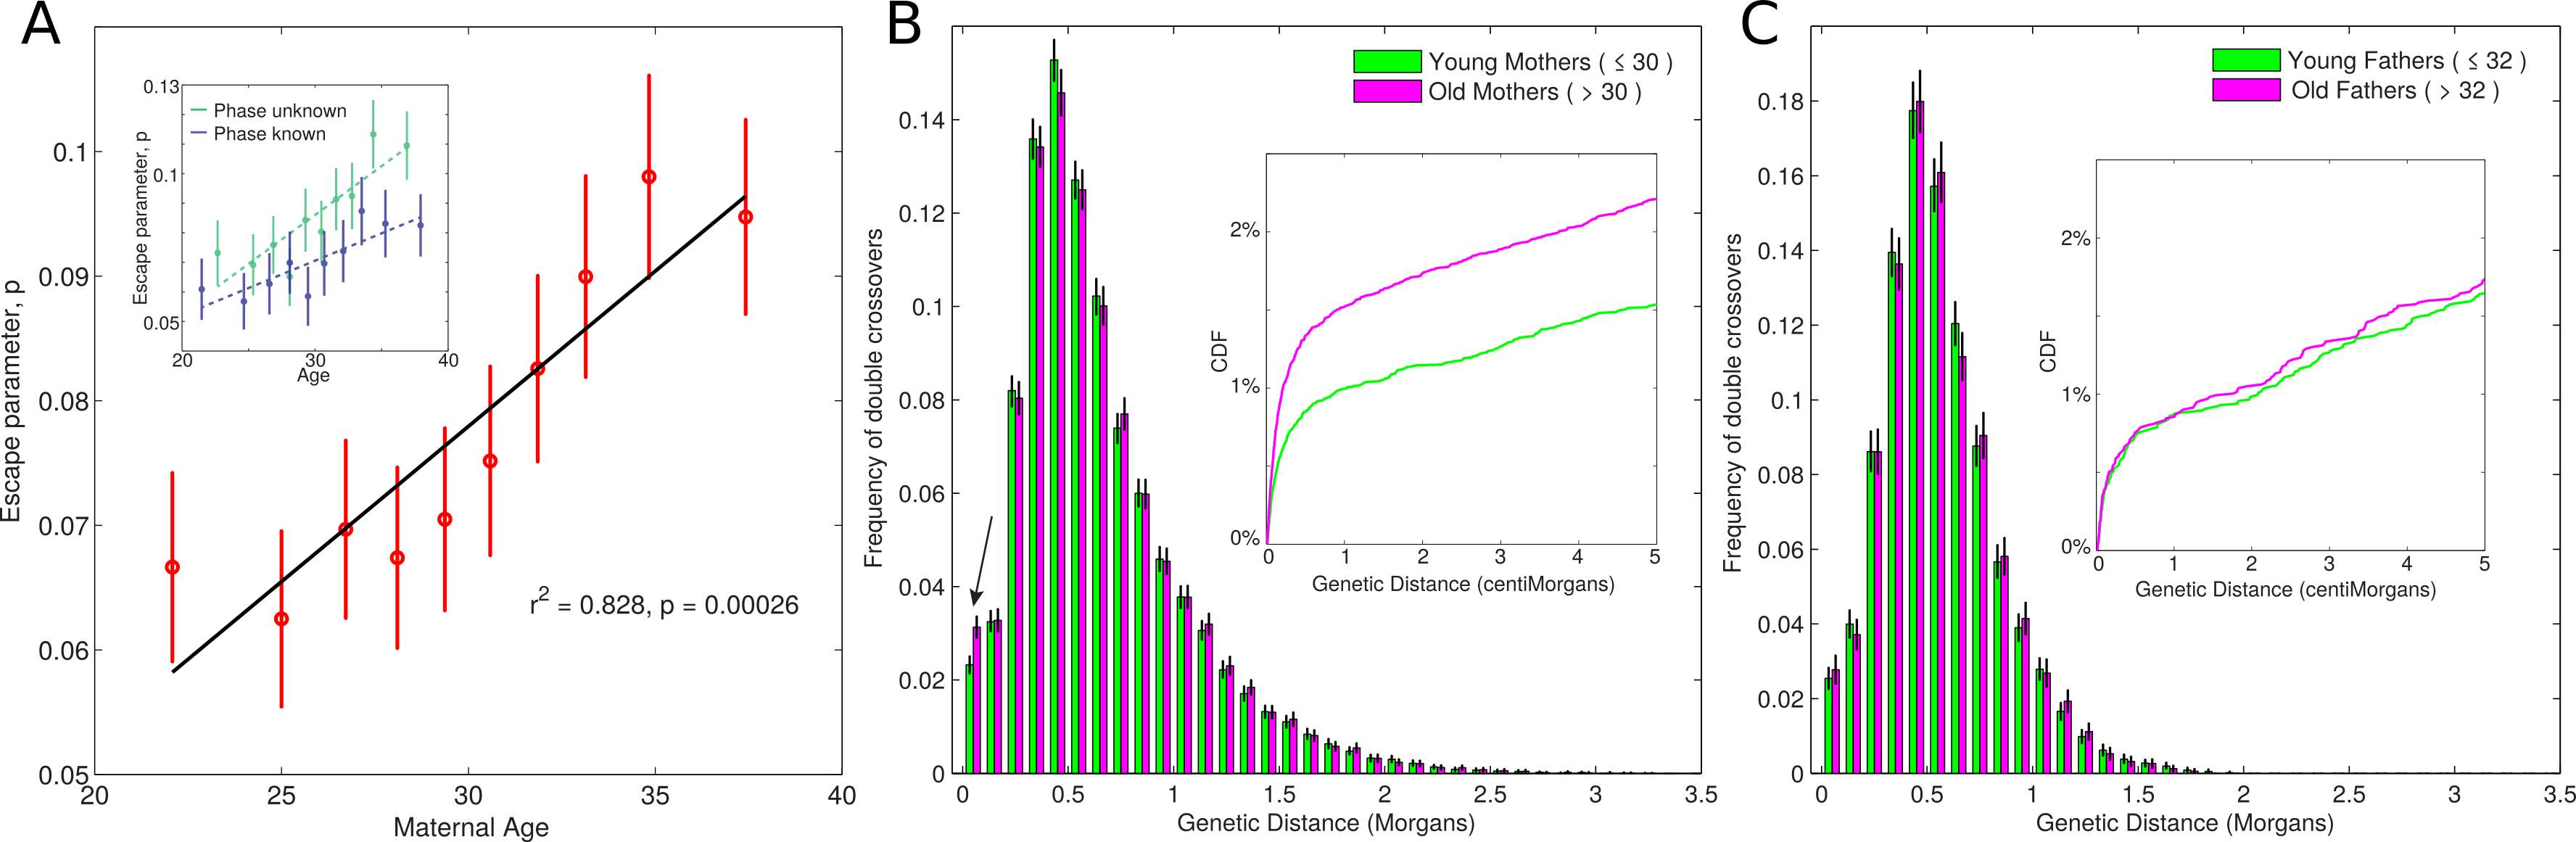
\includegraphics[width=\textwidth]{cointEscape/figs/Figure4.png}
    %\vspace{-20pt}
    \captionTitle{\textbf{Number of autosome recombination events verses parental age}}{
        for females (left) and males (right). 
        A linear least-squares fit is indicated by a black line.
        The least-squares fit equation given in the legend together with a p-value for the non-constant term.   
       \label{fig:cointFS6}}
\end{figure}

\begin{figure}[!h]
    %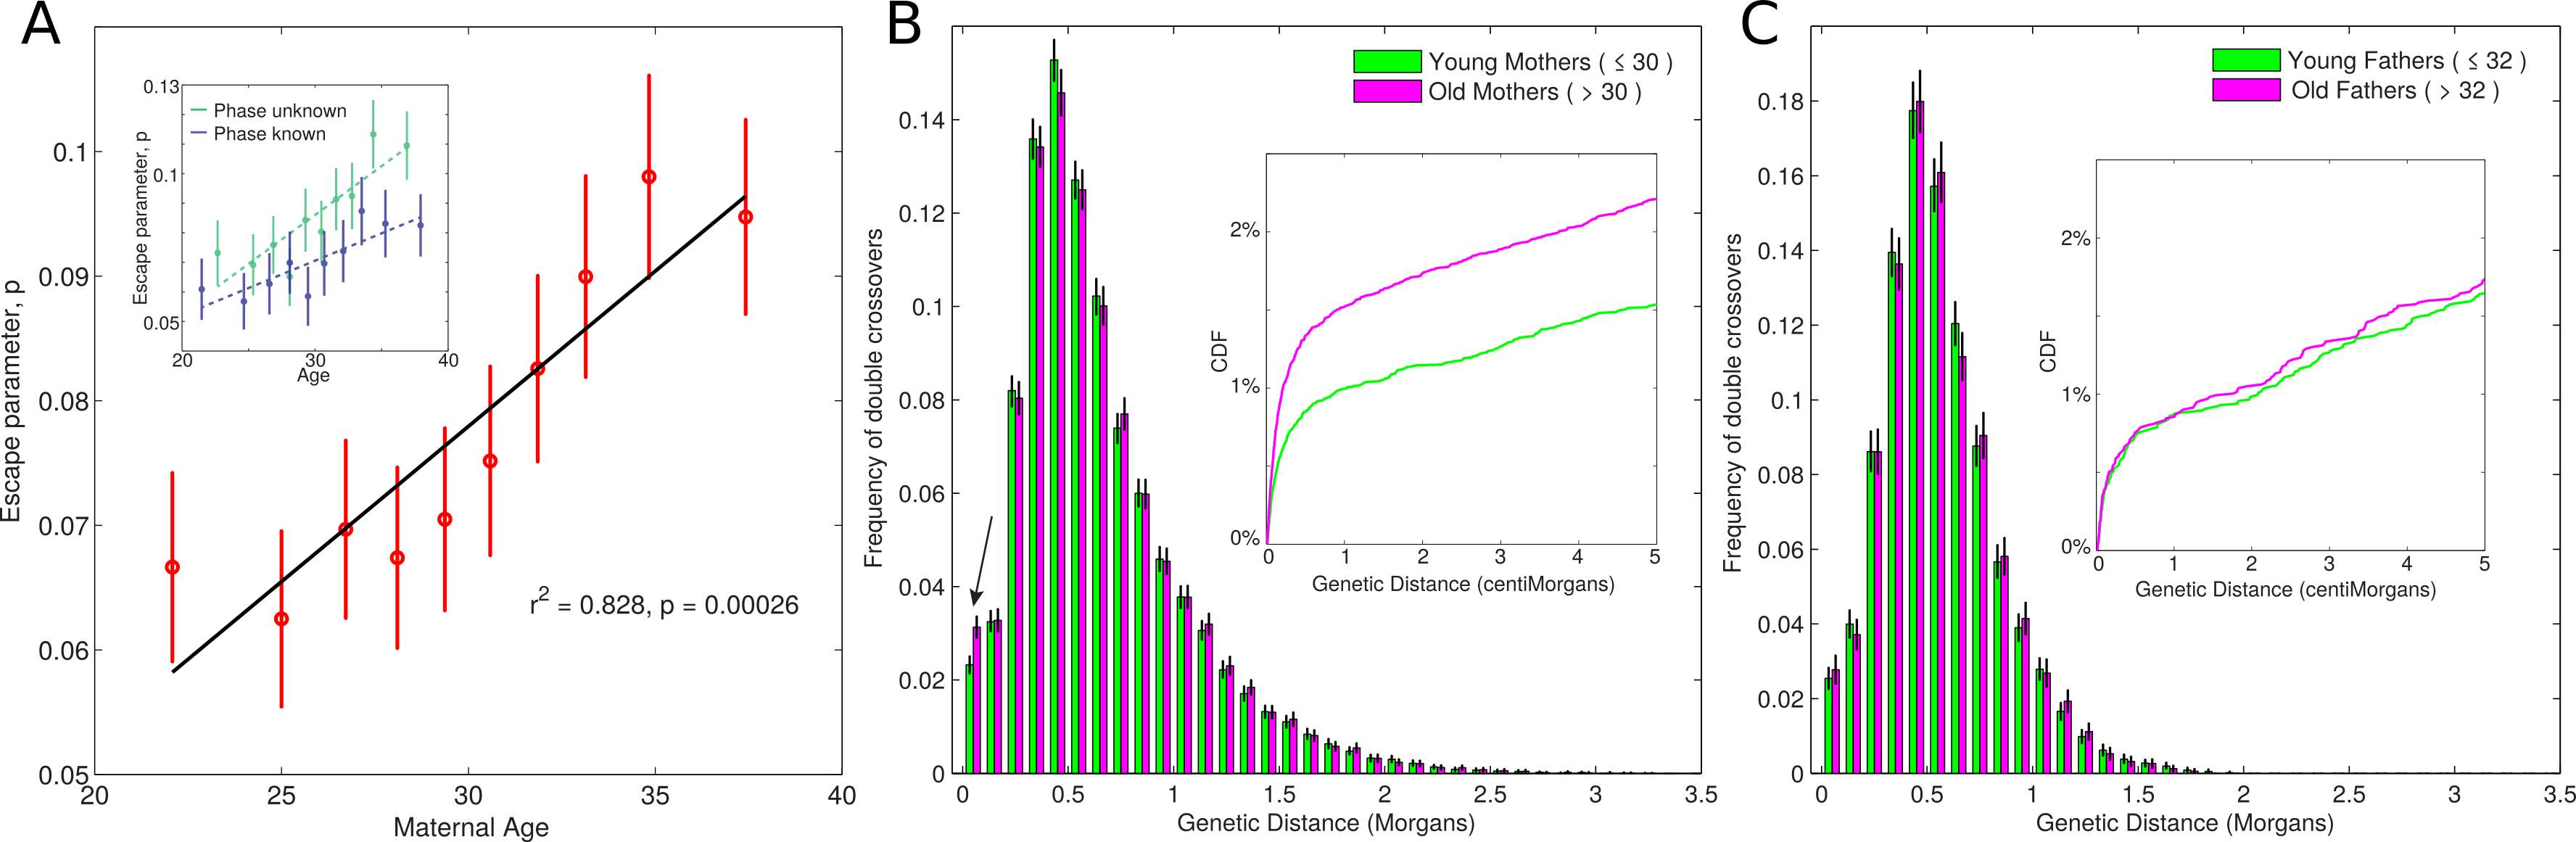
\includegraphics[width=\textwidth]{cointEscape/figs/Figure4.png}
    %\vspace{-20pt}
    \caption[\textbf{Hotspot usage between sexes.}]{
        A) Hotspot usage estimated in females (left) and males(right). 
        The MLE estimate for each individual is indicated by a circle, with a 95\% confidence interval indicated by the shaded area.
        The median MLE estimate for each sex is indicated by a vertical black line.
        B) Hotspot usage by parental age for females(left) and males (right).
        For each plot a logistic regression is also shown, with the p-value for the non-constant term given in the title.  
       \label{fig:cointFS7}}
\end{figure}

\begin{figure}[!h]
    %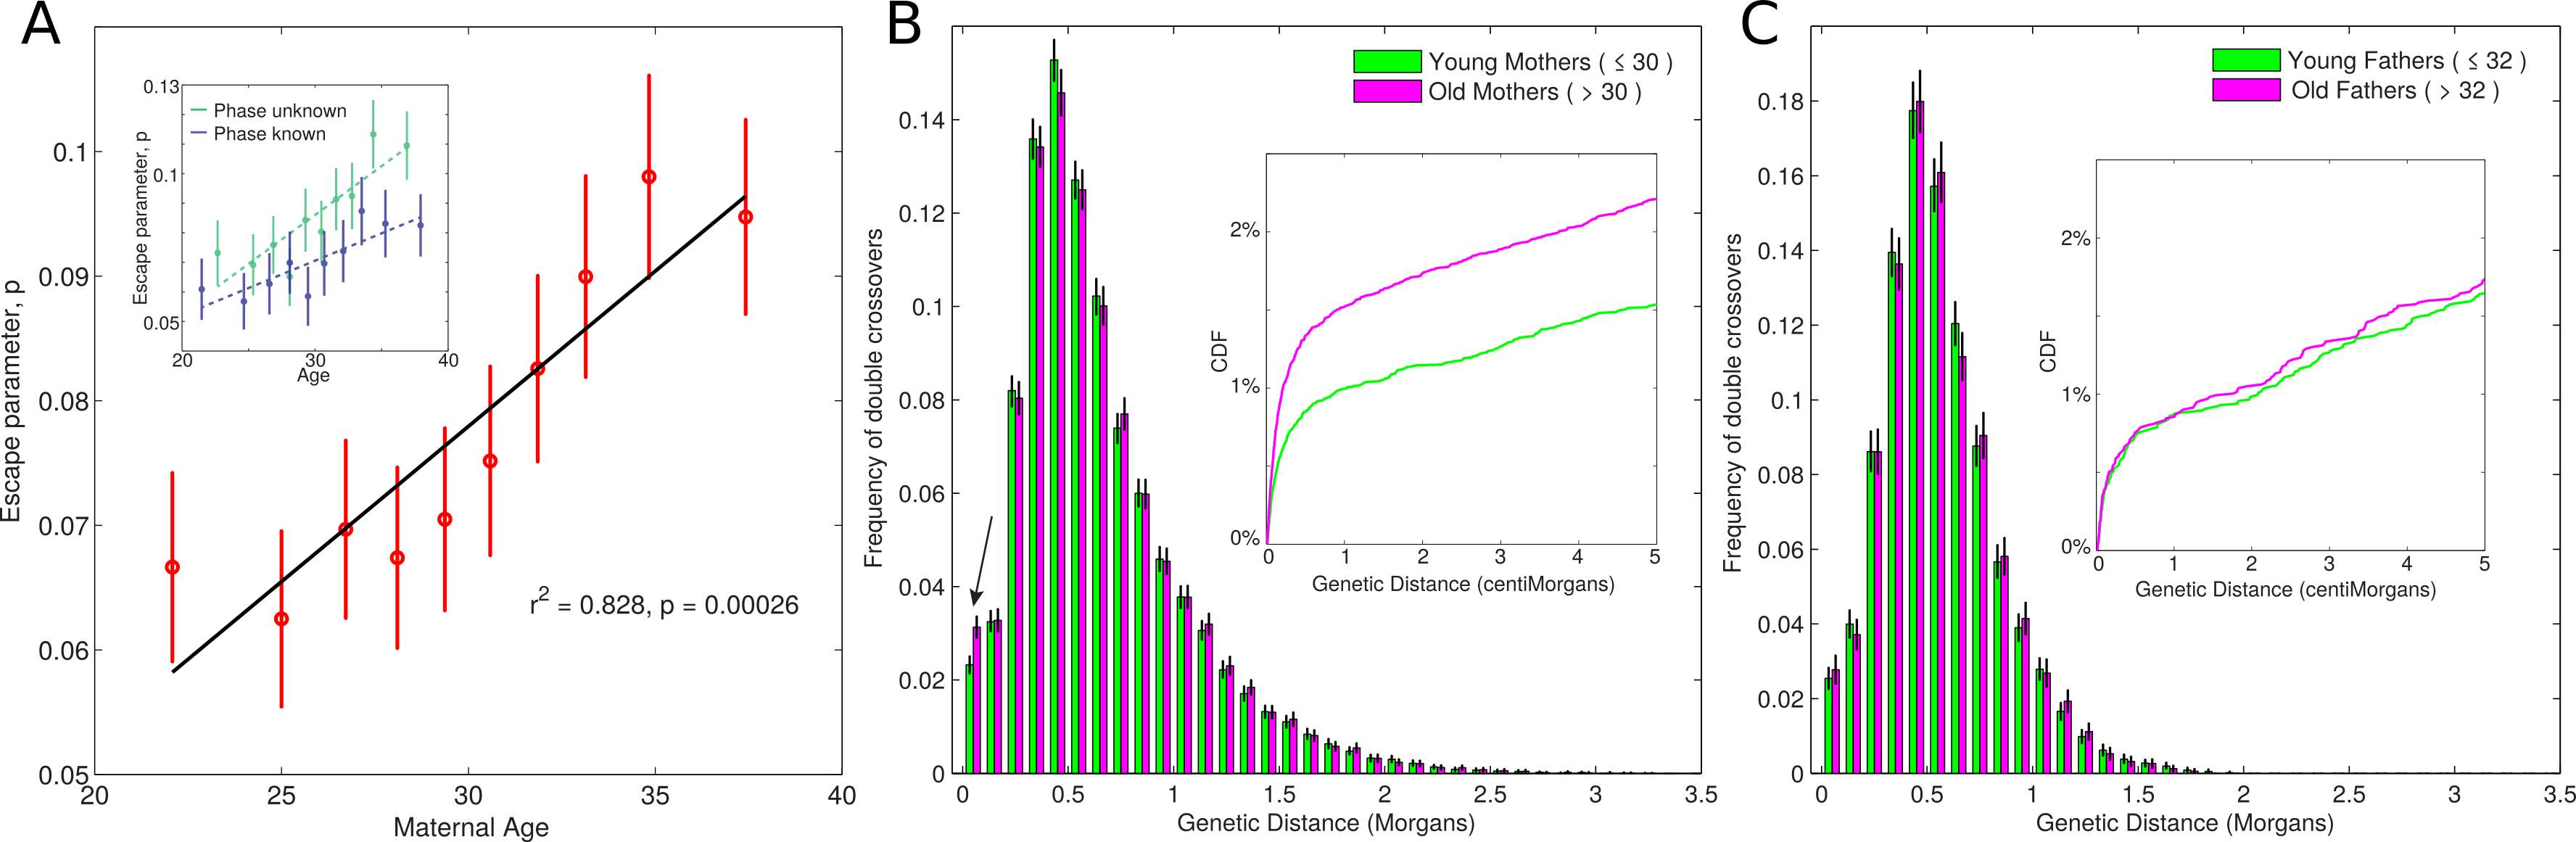
\includegraphics[width=\textwidth]{cointEscape/figs/Figure4.png}
    %\vspace{-20pt}
    \caption[\textbf{The relationship between map length and interference parameters.}]{ 
        A) The relationship between chromosome map length and the interference parameter, $\nu$.
        B) The relationship between chromosome map length and the escape parameter, $p$.
        Linear fits are shown for females (red), males (blue), and the data combined across sexes (black).
        In both plots, the chr21 estimate in males has been excluded.  
       \label{fig:cointFS8}}
\end{figure}

\begin{figure}[!h]
    %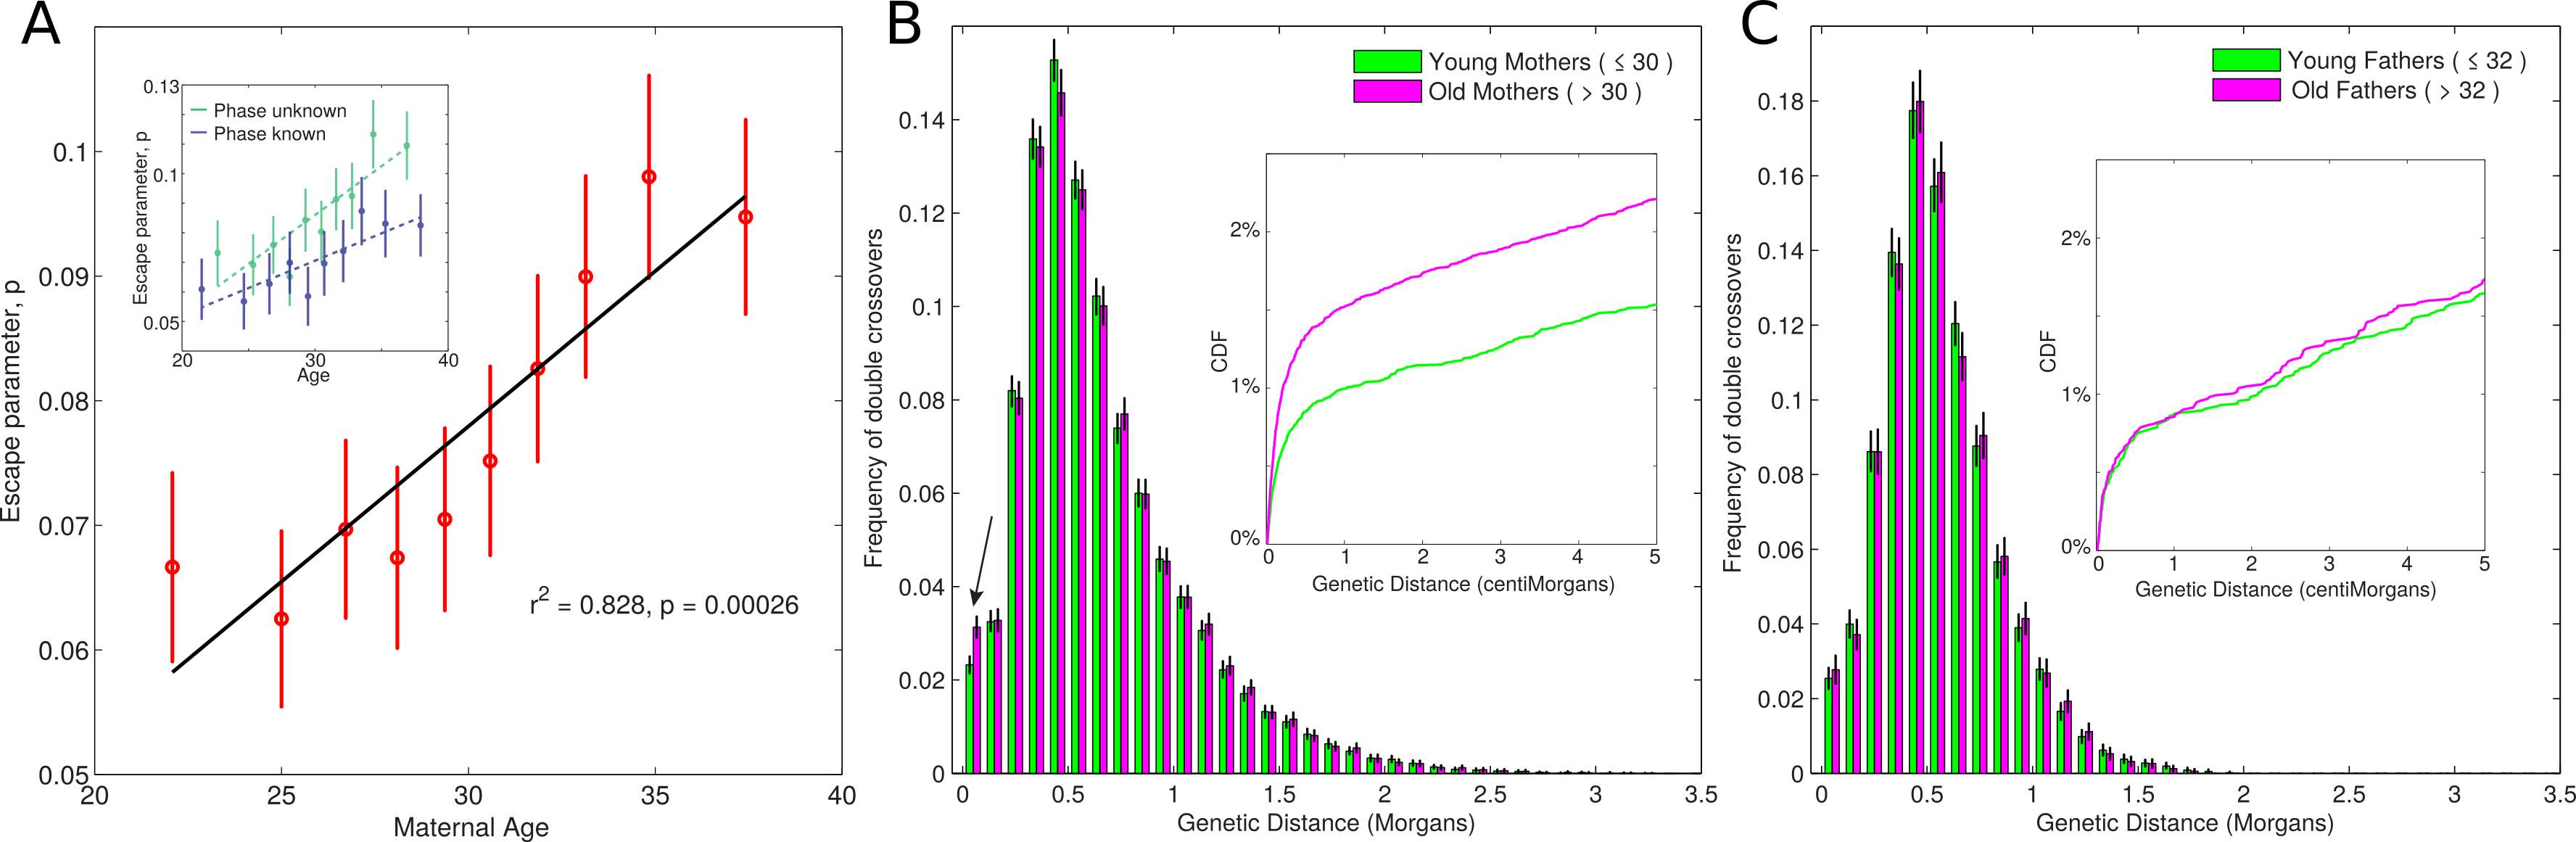
\includegraphics[width=\textwidth]{cointEscape/figs/Figure4.png}
    %\vspace{-20pt}
    \captionTitle{\textbf{Interference parameters as a function of age.}}{
        Females and males are shown on the top and bottom rows respectively. 
        Estimates of the interference parameter, $\nu$, are shown on the left, whereas estimates of the escape parameter, $p$, are shown on the right.
        Error bars show 95\% confidence intervals.  
       \label{fig:cointFS9}}
\end{figure}

\begin{figure}[!h]
    %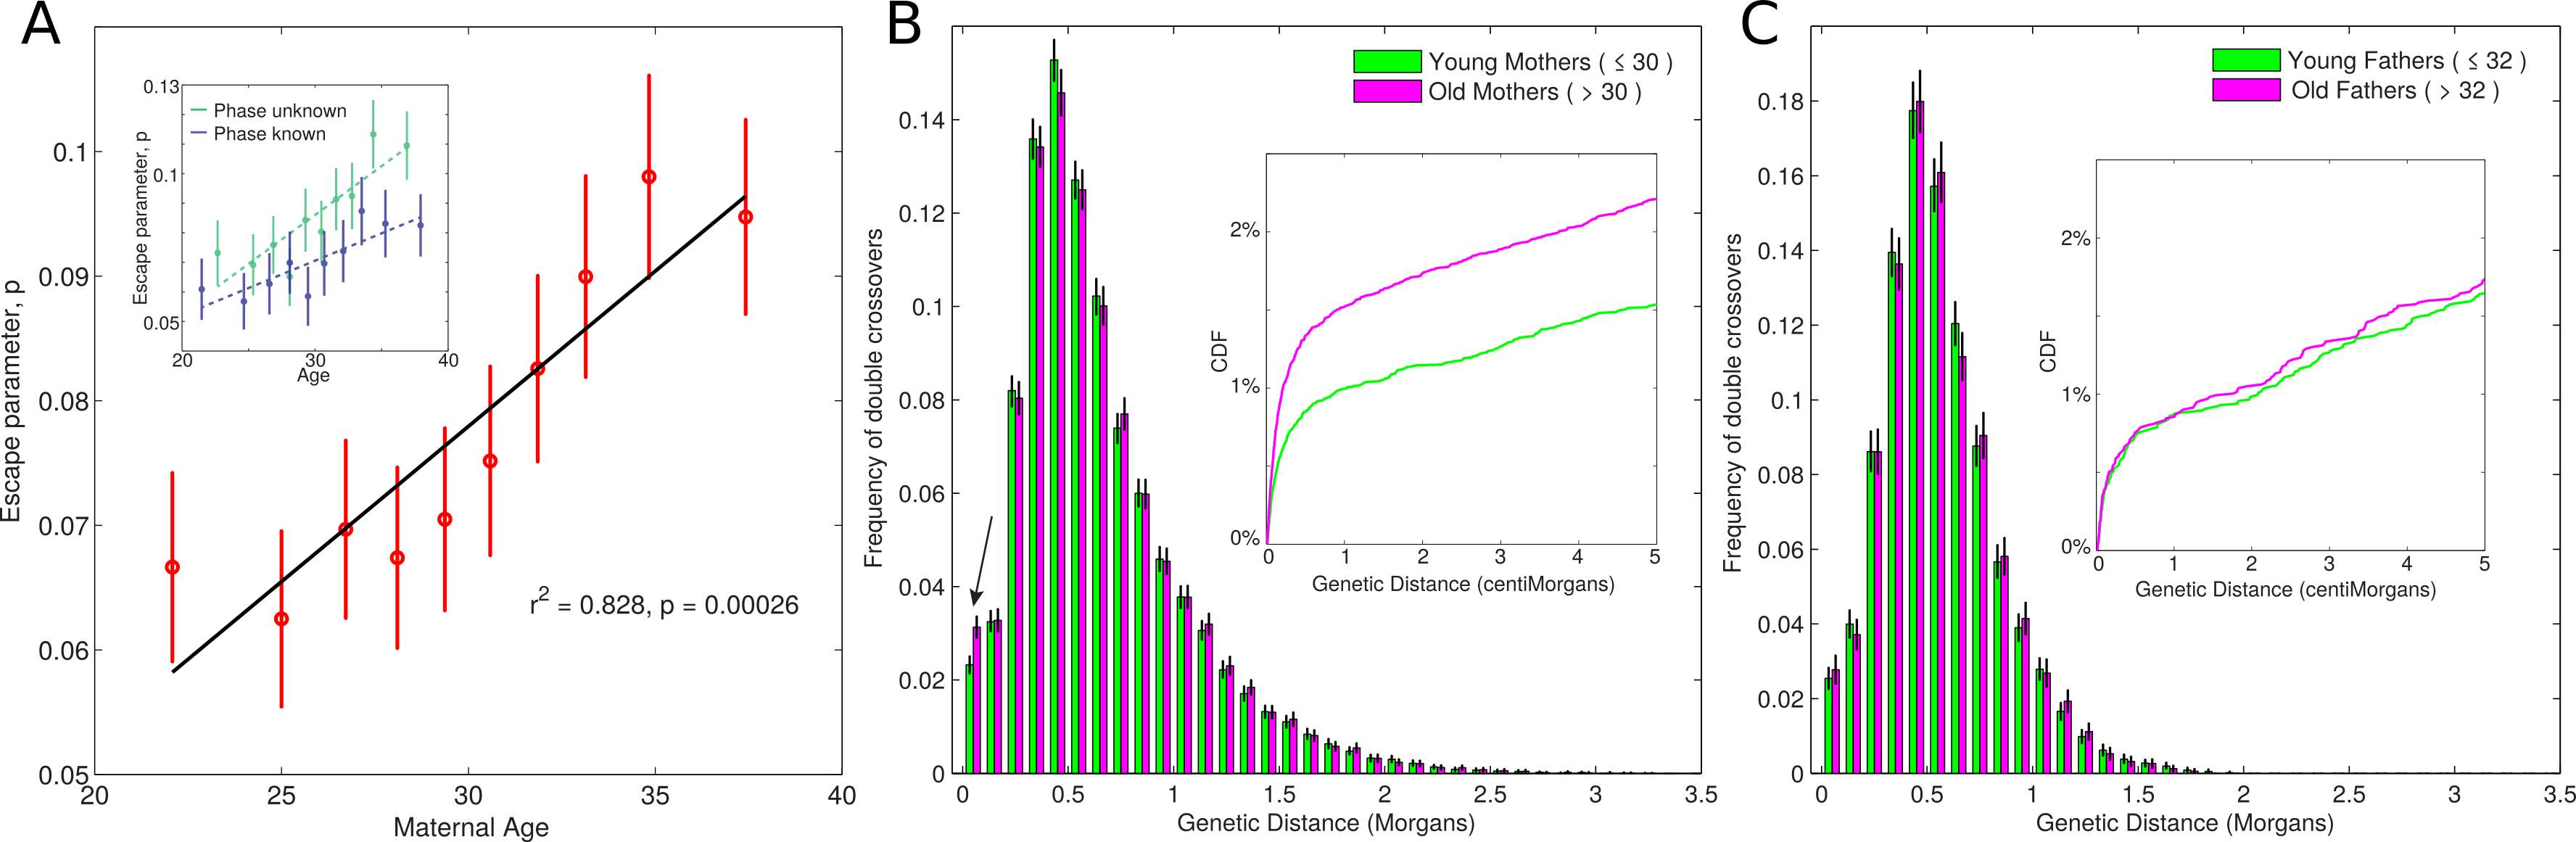
\includegraphics[width=\textwidth]{cointEscape/figs/Figure4.png}
    %\vspace{-20pt}
    \captionTitle{\textbf{Interference parameters by age}}{,
        having divided the data in 5 or 20 age quantiles.
        Error bars show 95\% confidence intervals.  
       \label{fig:cointFS10}}
\end{figure}

\begin{figure}[!h]
    %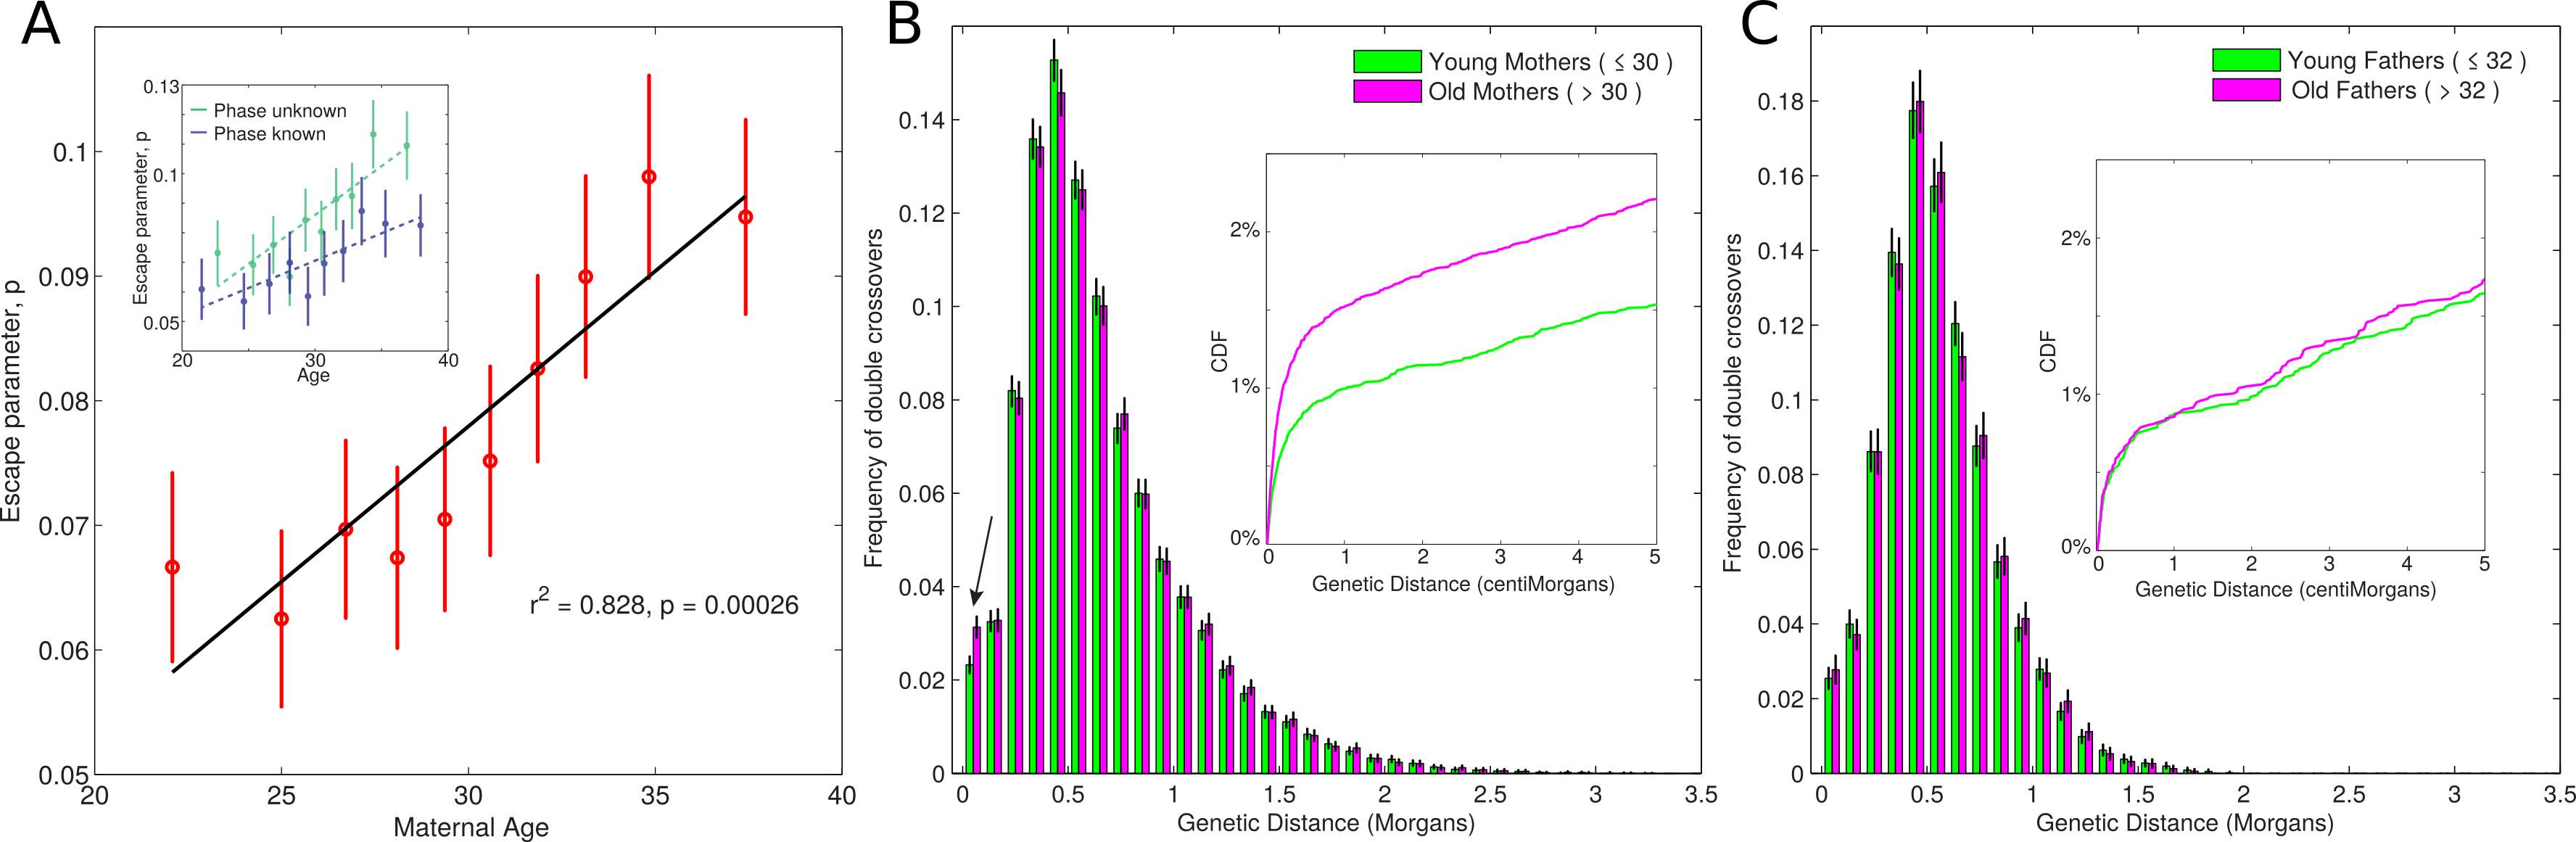
\includegraphics[width=\textwidth]{cointEscape/figs/Figure4.png}
    %\vspace{-20pt}
    \caption{\textbf{Interference parameters by age and phase.}}{ 
        Interference parameters by age, having estimated the interference parameters for phase-known and phase-unknown groups separately.  
       \label{fig:cointFS11}}
\end{figure}

\begin{figure}[!h]
    %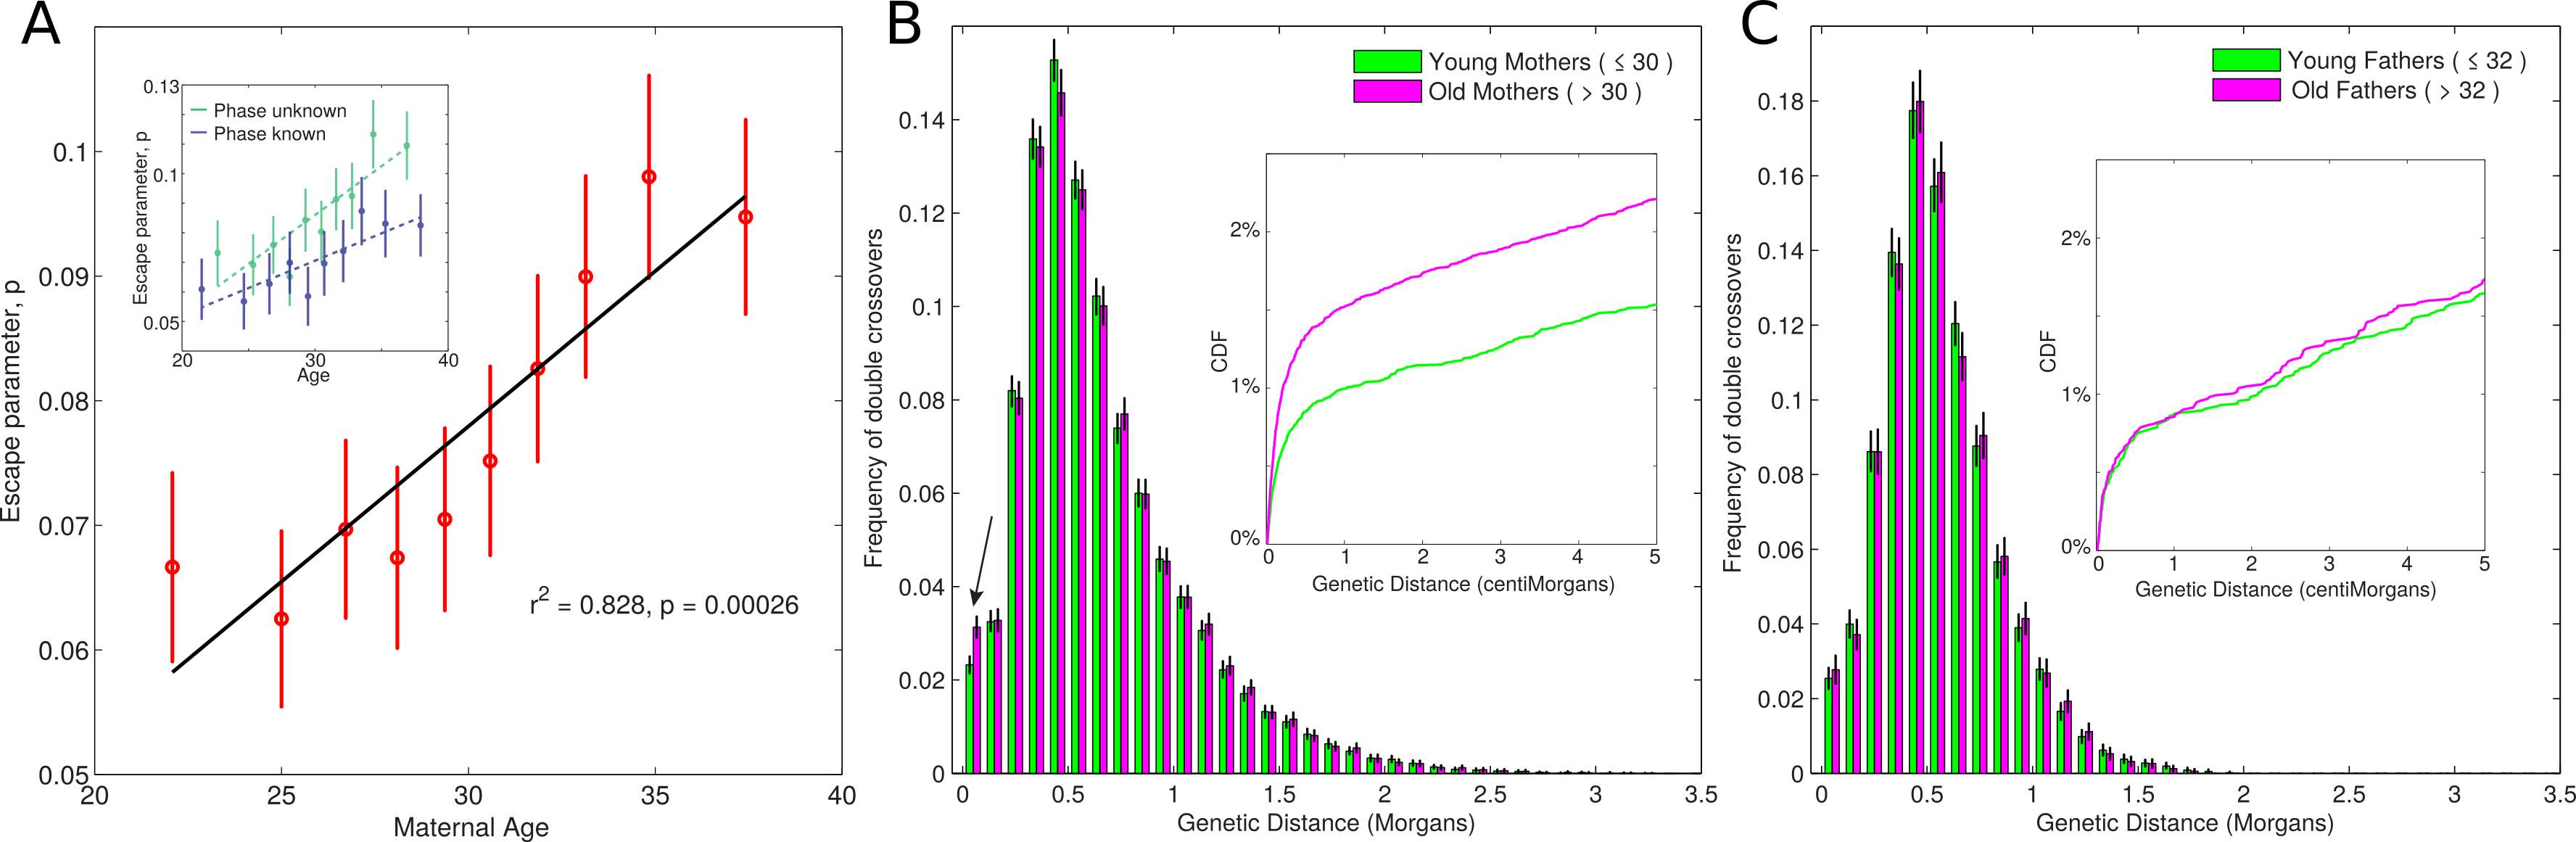
\includegraphics[width=\textwidth]{cointEscape/figs/Figure4.png}
    %\vspace{-20pt}
    \captionTitle{\textbf{Interference parameters as a function of age, following stratified sampling.}}{
        Females and males are shown on the top and bottom rows respectively.
        Estimates of the interference parameter, $\nu$, are shown on the left, whereas estimates of the escape parameter, $p$, are shown on the right.
        Error bars show 95\% confidence intervals.  
       \label{fig:cointFS12}}
\end{figure}

\begin{figure}[!h]
    %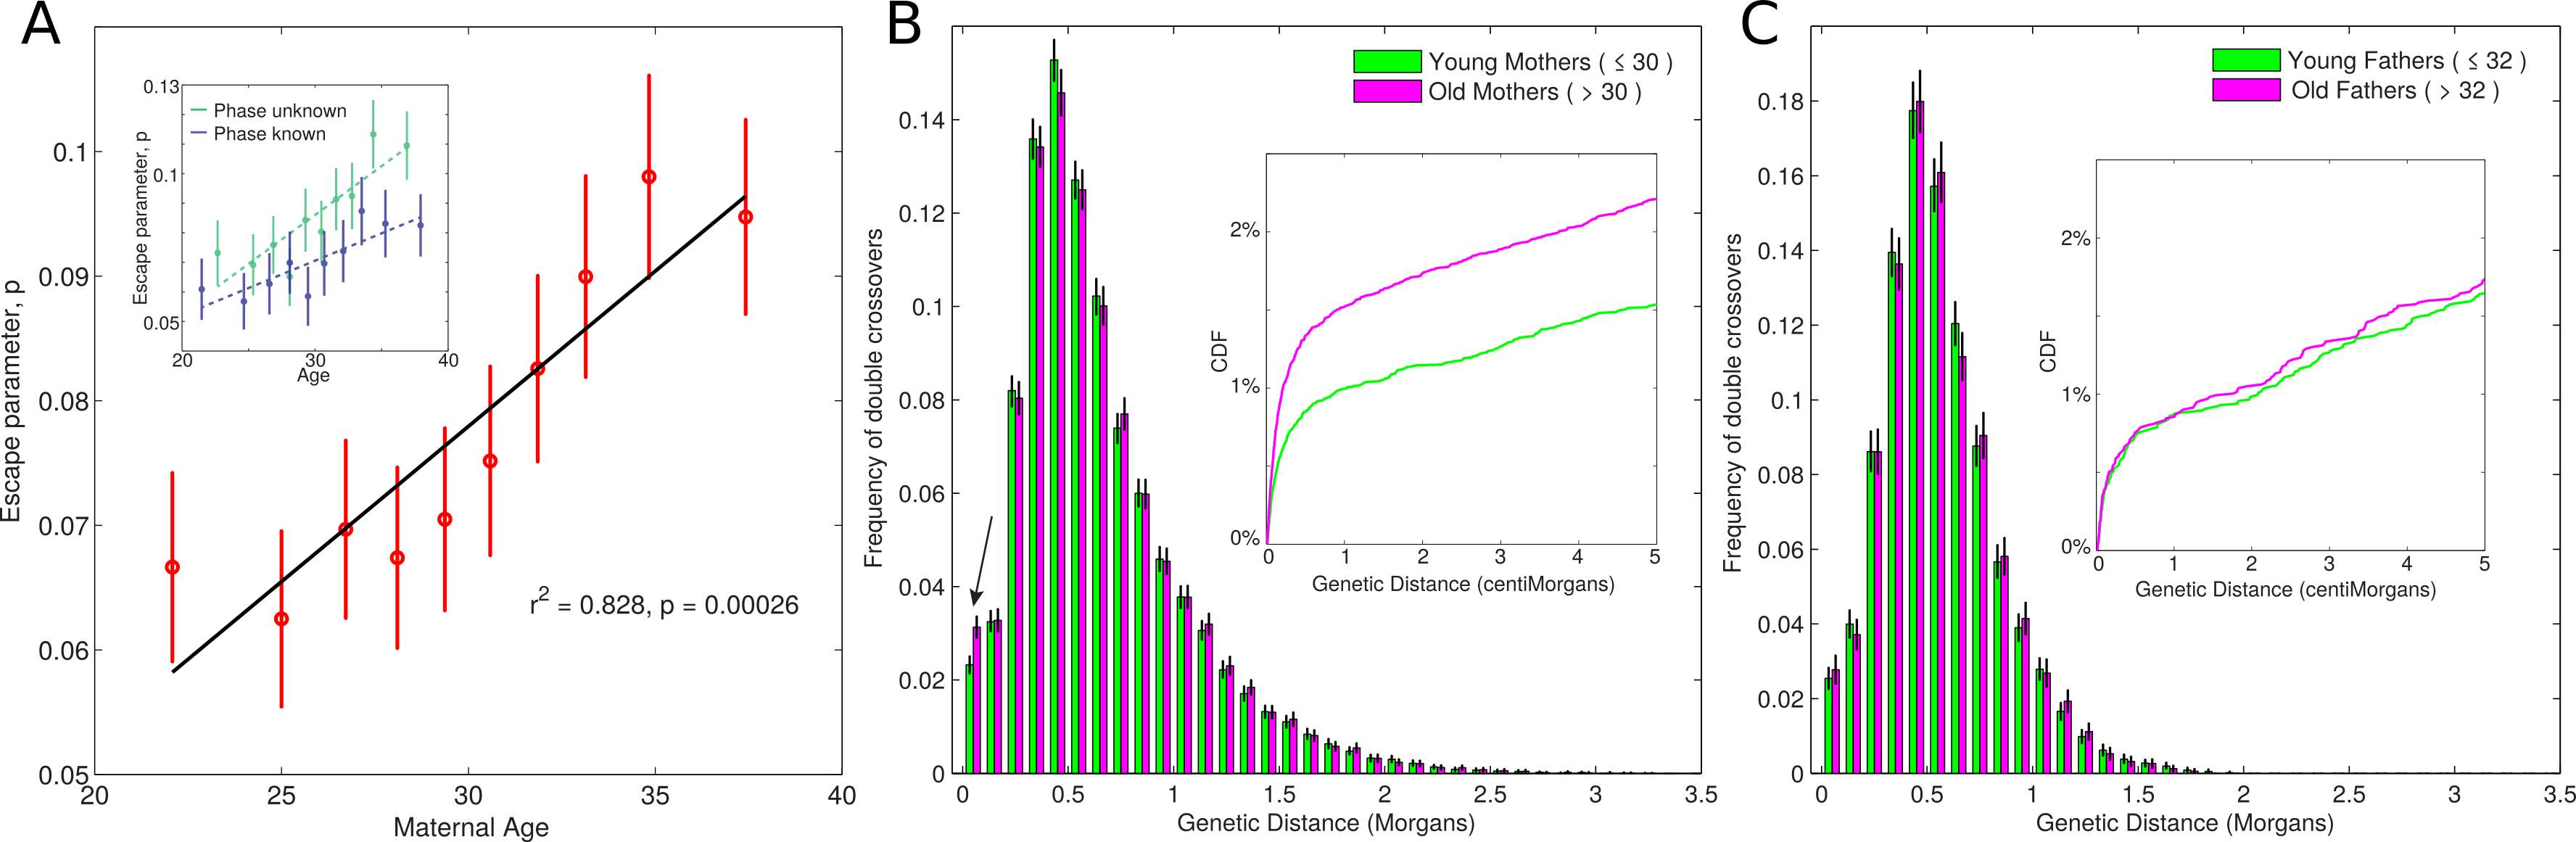
\includegraphics[width=\textwidth]{cointEscape/figs/Figure4.png}
    \vspace{-20pt}
    \captionTitle{\textbf{Model fit for tightly clustered events}}{
        in females (A) and males (B).
        The figure shows the empirical cumulative distribution function for young (green line) and old (magenta line) mothers/fathers, and compares to that obtained via simulation under the interference free model (black dotted line), the Gamma simple interference model (black dashed line), and the Housworth-Stahl interference escape model (solid black line), with parameters were taken from Supplementary Table 7.
        The figure is shown on a log-log scale to emphasize the short inter-crossover distances.  
       \label{fig:cointFS13}}
\end{figure}

\begin{figure}[!h]
    %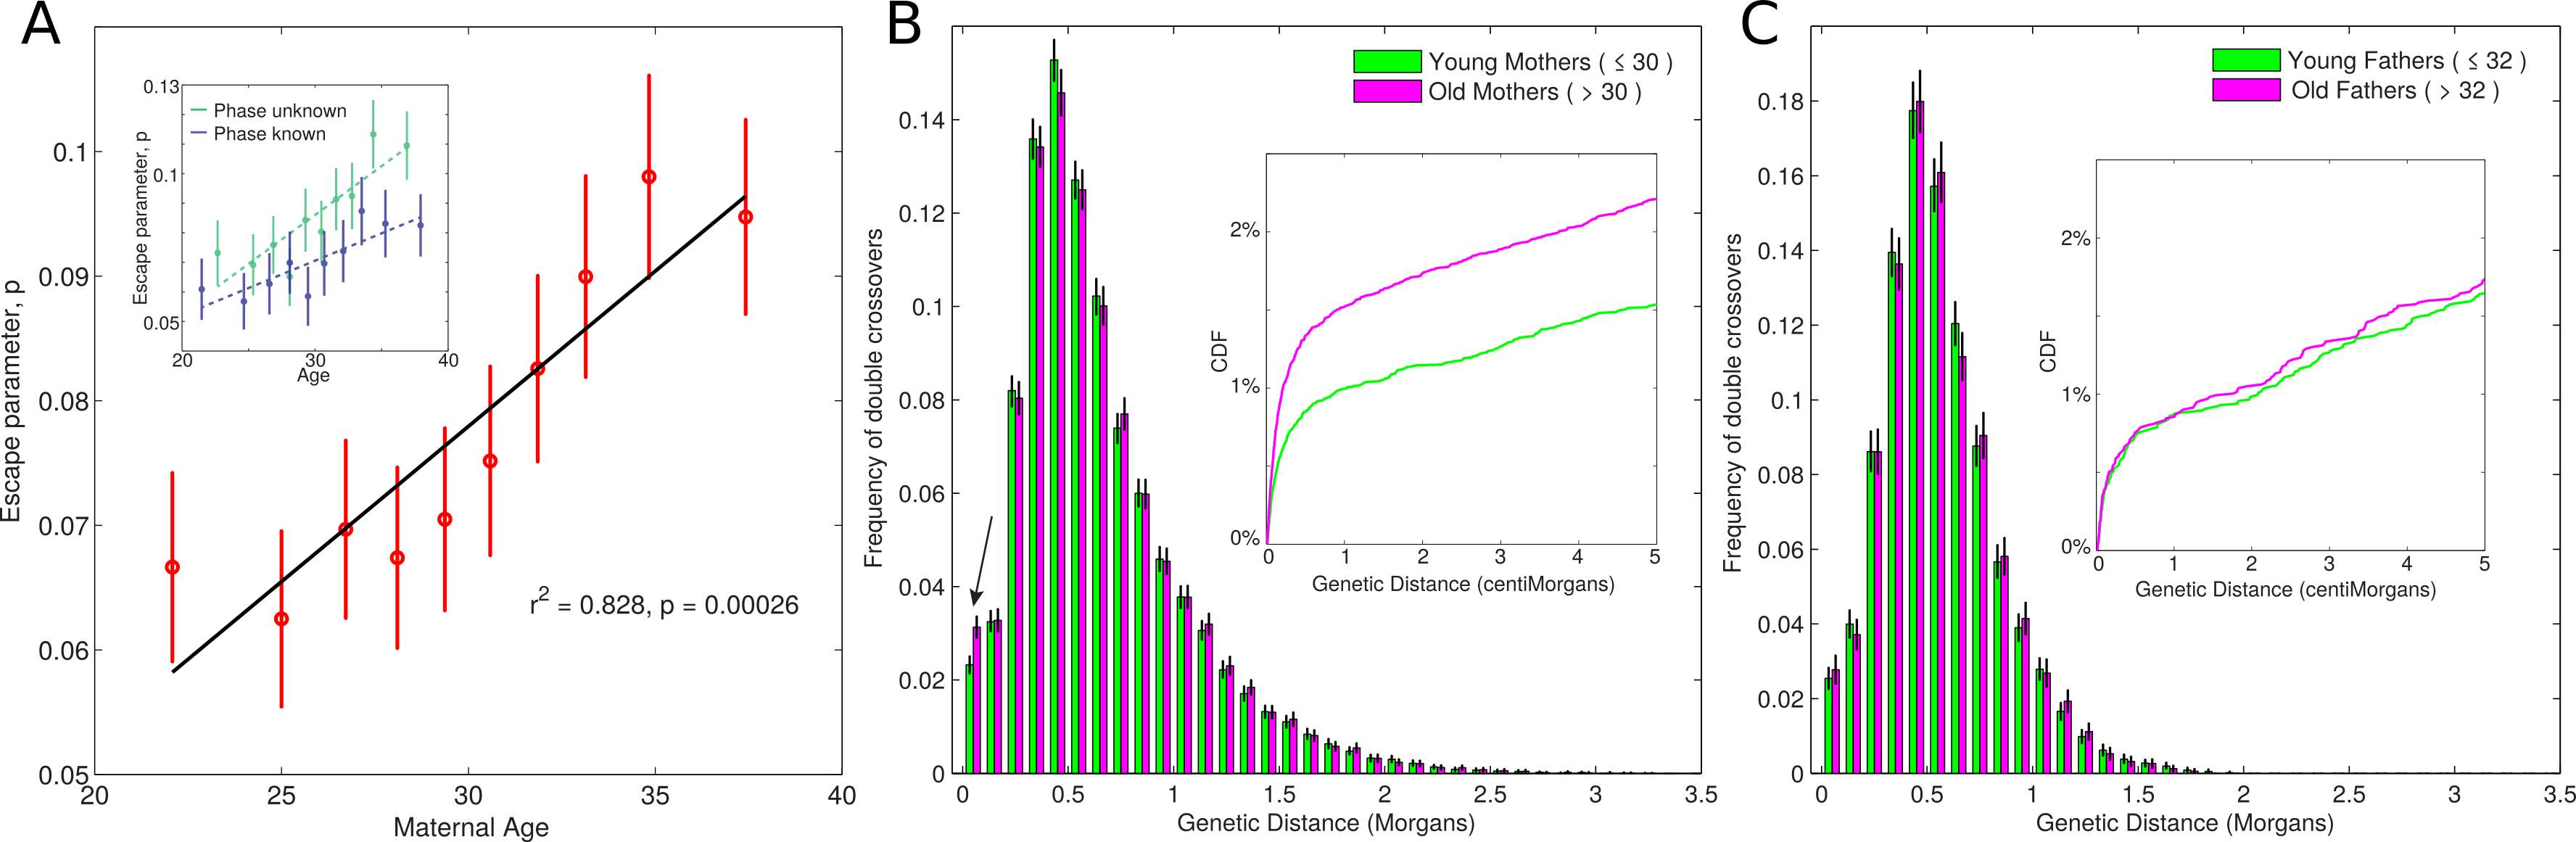
\includegraphics[width=\textwidth]{cointEscape/figs/Figure4.png}
    \vspace{-20pt}
    \captionTitle{\textbf{Interference parameters estimated for a strictly filtered dataset.}}{
        In this case, all crossover events were required at least 10 supporting informative sites (compared to 3 in the main dataset), no two events within a single family were allowed to be within 5 SNPs of each other (compared to 1 in the main dataset), and no more than 4 events within 1 Mb of each other were allowed across the whole dataset (and compared to 14 in the main dataset, which corresponds to the 99.9\textsuperscript{th} percentile).
        After this very strict filtering, the deviation from the Housworth-Stahl interference escape model is much less pronounced at short scales (right hand panels), but the association between interference escape and maternal  
        age remains strong (2\textsuperscript{nd} panel from top left).   
       \label{fig:cointFS14}}
\end{figure}


\subsection{Supplementary Tables}


\begin{table}[!h] \centering
    \begin{tabular}{|c|c|c|c|} 
        \hline Pedigree Type & Description & Before Filtering & After Filtering \\ \hline
        1 & 2 parents, 2 children & 3319 & 3307 \\
        2 & 2 parents, 3 children & 560 & 523 \\
        3 & 2 parents, 4 children & 89 & 80 \\
        4 & Quartet, with 2nd generation trio & 101 & 100 \\
        5 & Trio, with 2nd generation quartet & 201 & 199 \\
        \hline & \textbf{Total} & \textbf{4270} & \textbf{4209} \\
    \hline \end{tabular}
    \captionTitle{\textbf{Summary of dataset, before and after filtering.}}{
    \label{tab:cointTS1}}
\end{table}

\begin{table}[!h] \centering
    \begin{tabular}{|p{3cm}p{1.5cm}p{1.5cm}p{1.5cm}p{1.5cm}p{1.5cm}p{2cm}|}
        \hline 
    Population & Female \mbox{unphased} & Male \mbox{unphased} & Female phased & Male phased & Total Meioses & Percentage \\ \hline
    Europe & 5382 & 5508 & 1789 & 1641 & 14320 & 78.24\% \\
    Latino & 602 & 546 & 171 & 190 & 1509 & 8.25\% \\
    East Asia & 380 & 308 & 88 & 74 & 850 & 4.64\% \\
    None/Other & 198 & 268 & 68 & 109 & 643 & 3.51\% \\
    South Asia & 178 & 176 & 19 & 20 & 393 & 2.15\% \\
    African American & 152 & 152 & 34 & 36 & 374 & 2.04\% \\
    Middle East & 76 & 100 & 15 & 22 & 213 & 1.16\% \\
    \hline \textbf{Total} & \textbf{6968} & \textbf{7058} & \textbf{2184} & \textbf{2092} & \textbf{18302} & \textbf{100.00\%} \\
    \hline \end{tabular}
    \captionTitle{\textbf{Description of parental ancestry for each meiosis within the sample.}} {
    \label{tab:cointTS2}}
\end{table}

\begin{table}[!h] \centering
    \footnotesize
    \begin{tabular}{|cp{1.2cm}p{1.4cm}p{1.1cm}p{1.1cm}p{1.0cm}p{1.1cm}p{1.0cm}p{1.1cm}p{1.0cm}|}
        \hline 
Chrom & First Position (bp) & Last Position (bp) & Physical Length (Mb) & Female Map Length (cM) & Female Mean Rate (cM/Mb) & Male Map Length (cM) & Male Mean Rate (cM/Mb) & SexAvg Map Length (cM) & SexAvg Mean Rate (cM/Mb) \\ \hline
chr1 & 1,031,540 & 249,170,711 & 248.14 & 335.9 & 1.36 & 198.30 & 0.80 & 267.05 & 1.08 \\
chr2 & 118,913 & 242,763,542 & 242.64 & 316.45 & 1.31 & 184.64 & 0.76 & 250.52 & 1.03 \\
chr3 & 152,592 & 197,759,785 & 197.61 & 270.98 & 1.37 & 163.85 & 0.83 & 217.4 & 1.1 \\
chr4 & 167,596 & 190,787,660 & 190.62 & 260.11 & 1.37 & 145.79 & 0.76 & 202.93 & 1.06 \\
chr5 & 184,702 & 180,673,228 & 180.49 & 249.13 & 1.38 & 146.66 & 0.81 & 197.87 & 1.1 \\
chr6 & 188,937 & 170,777,087 & 170.59 & 236.64 & 1.39 & 140.88 & 0.83 & 188.74 & 1.11 \\
chr7 & 67,365 & 159,042,351 & 158.97 & 223.17 & 1.41 & 136.04 & 0.86 & 179.55 & 1.13 \\
chr8 & 200,898 & 146,235,564 & 146.03 & 210.94 & 1.45 & 122.41 & 0.84 & 166.64 & 1.14 \\
chr9 & 215,269 & 141,004,945 & 140.79 & 195.69 & 1.4 & 125.54 & 0.89 & 160.58 & 1.14 \\
chr10 & 162,102 & 135,402,200 & 135.24 & 207.86 & 1.54 & 129.91 & 0.96 & 168.86 & 1.25 \\
chr11 & 244,552 & 134,872,342 & 134.63 & 193.59 & 1.44 & 120.21 & 0.89 & 156.88 & 1.17 \\
chr12 & 216,039 & 133,684,321 & 133.47 & 200.36 & 1.51 & 131.20 & 0.98 & 165.75 & 1.24 \\
chr13 & 19,458,371 & 114,998,076 & 95.54 & 152.26 & 1.6 & 101.19 & 1.06 & 126.71 & 1.33 \\
chr14 & 20,445,905 & 107,233,999 & 86.79 & 137.22 & 1.59 & 97.29 & 1.12 & 117.24 & 1.35 \\
chr15 & 22,763,396 & 102,381,360 & 79.62 & 143.39 & 1.8 & 100.85 & 1.27 & 122.11 & 1.53 \\
chr16 & 143,503 & 90,102,384 & 89.96 & 157.29 & 1.75 & 102.03 & 1.13 & 129.64 & 1.44 \\
chr17 & 84,782 & 81,025,393 & 80.94 & 152.87 & 1.9 & 106.23 & 1.31 & 129.53 & 1.6 \\
chr18 & 218,695 & 77,955,378 & 77.74 & 140.06 & 1.81 & 97.80 & 1.26 & 118.91 & 1.53 \\
chr19 & 288,246 & 59,058,083 & 58.77 & 117.8 & 2.01 & 99.42 & 1.69 & 108.59 & 1.85 \\
chr20 & 100,699 & 62,892,739 & 62.79 & 118.9 & 1.9 & 99.00 & 1.58 & 108.93 & 1.73 \\
chr21 & 14,807,136 & 47,978,421 & 33.17 & 74.34 & 2.24 & 51.76 & 1.58 & 63.04 & 1.9 \\
chr22 & 17,152,611 & 51,165,664 & 34.01 & 78.16 & 2.31 & 63.30 & 1.86 & 70.71 & 2.08 \\
chrX & 2,737,282 & 154,408,041 & 151.67 & 179.02 & 1.18 &  &  &  &  \\
PAR1 & 178,624 & 2,689,575 & 2.51 & 2.73 & 1.16 & 42.94 & 17.17 & 22.75 & 9.06 \\
PAR2 & 154,984,651 & 155,227,607 & 0.24 & 0.05 & 0.34 & 0.33 & 1.35 & 0.19 & 0.79 \\
        \hline Genome &&& 2932.98 & 4354.91 & 1.48 & 2707.55 & 0.92 & 3441.11 & 1.17 \\
    \hline \end{tabular}
    \captionTitle{\textbf{Properties of the map estimated from 23andMe data.}}{
        Recombination fractions were converted to genetic map distances using the Haldane map function.  
    \label{tab:cointTS3}}
\end{table}

\begin{table}[!h] \centering
    \footnotesize
    \begin{tabular}{|cccccccc|}
        \hline 
SNP & Chrom & Position & Alleles & P-value & Effect & 95\% CI & Gene Context \\ \hline
rs2001572 & chr14 & 20,767,868 & A/T & 1.50E-08 & 0.503 & [0.329,0.677] & [TTC5] \\
rs79621814 & chr4 & 1,089,268 & C/T & 2.90E-08 & -0.99 & [-1.340,-0.640] & [RNF212] \\
rs11624006 & chr14 & 91,961,188 & C/T & 2.80E-07 & -0.478 & [-0.660,-0.296] & [SMEK1] \\
rs72631326 & chr17 & 65,769,087 & C/T & 4.40E-07 & 0.959 & [0.587,1.331] & NOL11--[]--BPTF \\
rs11932663 & chr4 & 184,458,083 & A/G & 5.10E-07 & 0.622 & [0.380,0.865] & ING2--[]---RWDD4 \\
rs17127442 & chr8 & 18,779,787 & C/T & 5.10E-07 & -0.537 & [-0.746,-0.327] & [PSD3] \\
rs1879904 & chr11 & 82,076,387 & C/T & 6.80E-07 & -0.507 & [-0.707,-0.307] & []---FAM181B \\
    \hline \end{tabular}
    \captionTitle{\textbf{Variants associated with total number of recombination events.}}{
        Linear regression model tested as N\_events $\sim$ sex + age + pc.0 + pc.1 + pc.2 + pc.3 + pc.4 + genotype. 
        Association tests conducted using only individuals found to have $\ge$ 97\% European ancestry. 
    \label{tab:cointTS4}}
\end{table}

\clearpage 

\begin{table}[!h] \centering
    \footnotesize
    \begin{tabular}{|cccccccc|}
        \hline 
SNP & Chrom & Position & Alleles & P-value & Effect & 95\% CI & Gene Context \\ \hline
rs73742307 & chr5 & 23,534,421 & C/T & 7.90E-184 & 0.16 & [0.149,0.170] & PRDM9-[]---CDH10 \\
rs78474856 & chr20 & 1,450,623 & C/G & 6.10E-07 & -0.021 & [-0.029,-0.013] & NSFL1C-[]-SIRPB2 \\
rs62078596 & chr17 & 53,906,496 & C/T & 8.50E-07 & 0.013 & [0.008,0.018] & PCTP--[]---ANKFN1 \\
rs8134126 & chr21 & 28,401,705 & C/T & 1.00E-06 & -0.01 & [-0.013,-0.006] & ADAMTS5--[] \\
rs138108783 & chr1 & 119,711,419 & A/G & 1.40E-06 & 0.274 & [0.163,0.385] & WARS2--[]---HAO2 \\
    \hline \end{tabular}
    \captionTitle{\textbf{Variants associated with hotspot usage.}}{
        Linear regression model tested as hotspot\_usage $\sim$ sex + age + pc.0 + pc.1 + pc.2 + pc.3 + pc.4 + genotype.
        Association tests conducted using only individuals found to have $\ge$ 97\% European ancestry.  
    \label{tab:cointTS5}}
\end{table}

\begin{table}[!h] \centering
    %\footnotesize
    \begin{tabular}{|cp{1.5cm}p{1.5cm}p{1.5cm}p{1.5cm}cp{2cm}|}
        \hline 
        Population & Female sample size* & Male sample size* & Female median hotspot usage & Male median hotspot usage & Difference & p-value (Mann-Whitney U) \\ \hline
        Europe & 3329 & 3325 & 62.96\% & 67.12\% & 4.16\% & 4.93E-40 \\
        Latino & 362 & 341 & 61.15\% & 66.84\% & 5.68\% & 1.36E-09 \\
        East Asia & 221 & 180 & 60.38\% & 67.56\% & 7.18\% & 5.67E-06 \\
        South Asia & 97 & 95 & 61.65\% & 66.35\% & 4.71\% & 0.00494563 \\
        Middle East & 88 & 88 & 59.52\% & 61.26\% & 1.74\% & 0.284789 \\
        African American & 43 & 57 & 61.37\% & 65.37\% & 4.00\% & 0.135323 \\
        \hline All & 5668 & 5621 & 0.6268 & 0.67255 & 0.04575 & 1.06E-69 \\
    \hline \end{tabular}
\captionTitle{\textbf{Differences in hotspot usage between males and females}}{, partitioned by population.
        *The sample size represents the number estimated $\alpha$s, with one estimate for each meiosis from phase-known parents, and a single estimate for phase-unknown parents.  
    \label{tab:cointTS6}}
\end{table}

\clearpage 
\begin{table}[!h] \centering
    \scriptsize
    \begin{tabular}{|c|p{1.1cm}p{1.2cm}p{1.3cm}|cccccc|} \hline 
    \multicolumn{10}{|l|}{\textbf{Females}} \\ \hline
    & \multicolumn{3}{c|}{\textbf{Gamma model (no escape)}} & \multicolumn{6}{c|}{\textbf{Escape model}} \\
    & Phase known & Phase \mbox{unknown} & Weighted mean & 
    \multicolumn{2}{c}{Phase known} & \multicolumn{2}{c}{Phase unknown} & \multicolumn{2}{c|}{Weighted mean} \\
    Chrom & $\nu$ & $\nu$ & $\nu$ & $\nu$ & p & $\nu$ & p & $\nu$ & p \\ \hline
    chr1 & 2.749 & 3.211 & 2.952 & 6.045 & 0.067 & 6.711 & 0.079 & 6.384 & 0.073 \\
    chr2 & 2.390 & 3.035 & 2.643 & 6.499 & 0.064 & 6.902 & 0.076 & 6.718 & 0.070 \\
    chr3 & 2.328 & 2.653 & 2.473 & 6.489 & 0.072 & 6.612 & 0.089 & 6.556 & 0.081 \\
    chr4 & 3.074 & 3.956 & 3.414 & 5.981 & 0.042 & 6.036 & 0.047 & 6.009 & 0.044 \\
    chr5 & 3.289 & 3.824 & 3.526 & 6.582 & 0.044 & 6.941 & 0.065 & 6.753 & 0.052 \\
    chr6 & 2.893 & 2.864 & 2.878 & 7.221 & 0.055 & 7.395 & 0.086 & 7.314 & 0.069 \\
    chr7 & 3.007 & 2.826 & 2.902 & 7.435 & 0.048 & 7.289 & 0.090 & 7.360 & 0.065 \\
    chr8 & 1.395 & 2.014 & 1.566 & 8.073 & 0.165 & 6.615 & 0.184 & 7.141 & 0.175 \\
    chr9 & 1.760 & 2.590 & 2.007 & 6.168 & 0.095 & 7.096 & 0.113 & 6.586 & 0.105 \\
    chr10 & 2.548 & 4.228 & 2.971 & 7.561 & 0.066 & 7.039 & 0.056 & 7.260 & 0.061 \\
    chr11 & 2.485 & 2.829 & 2.645 & 7.466 & 0.065 & 8.240 & 0.084 & 7.818 & 0.074 \\
    chr12 & 2.979 & 3.896 & 3.323 & 7.519 & 0.058 & 6.927 & 0.060 & 7.175 & 0.059 \\
    chr13 & 3.506 & 4.727 & 3.982 & 7.876 & 0.039 & 7.157 & 0.034 & 7.442 & 0.036 \\
    chr14 & 2.654 & 4.065 & 3.070 & 7.574 & 0.056 & 7.338 & 0.059 & 7.451 & 0.057 \\
    chr15 & 2.090 & 2.604 & 2.292 & 7.652 & 0.081 & 7.842 & 0.109 & 7.754 & 0.095 \\
    chr16 & 1.357 & 1.888 & 1.504 & 7.708 & 0.158 & 9.383 & 0.220 & 8.277 & 0.190 \\
    chr17 & 2.874 & 4.016 & 3.246 & 8.216 & 0.064 & 6.972 & 0.056 & 7.479 & 0.061 \\
    chr18 & 3.063 & 4.920 & 3.575 & 8.244 & 0.064 & 8.056 & 0.053 & 8.139 & 0.058 \\
    chr19 & 3.444 & 5.322 & 4.001 & 7.991 & 0.052 & 8.576 & 0.055 & 8.273 & 0.053 \\
    chr20 & 3.149 & 3.530 & 3.329 & 7.672 & 0.060 & 7.612 & 0.078 & 7.637 & 0.070 \\
    chr21 & 2.694 & 3.596 & 2.996 & 9.454 & 0.061 & 9.713 & 0.064 & 9.598 & 0.062 \\
    chr22 & 2.315 & 1.904 & 2.033 & 9.456 & 0.060 & 10.664 & 0.128 & 9.958 & 0.090 \\
    chrX & 1.959 & 2.151 & 2.050 & 6.439 & 0.089 & 5.886 & 0.110 & 6.129 & 0.100 \\
    Autosomes & 2.409 & 3.084 & 2.666 & 7.134 & 0.071 & 7.233 & 0.086 & 7.188 & 0.078 \\
    \hline\hline
    \multicolumn{10}{|l|}{\textbf{Males}} \\ \hline
    & \multicolumn{3}{c|}{\textbf{Gamma model (no escape)}} & \multicolumn{6}{c|}{\textbf{Escape model}} \\
    & Phase known & Phase \mbox{unknown} & Weighted mean & 
    \multicolumn{2}{c}{Phase known} & \multicolumn{2}{c}{Phase unknown} & \multicolumn{2}{c|}{Weighted mean} \\
    Chrom & $\nu$ & $\nu$ & $\nu$ & $\nu$ & p & $\nu$ & p & $\nu$ & p \\ \hline
    chr1 & 3.240 & 3.289 & 3.266 & 8.515 & 0.047 & 9.419 & 0.082 & 8.949 & 0.063 \\
    chr2 & 4.081 & 3.972 & 4.019 & 7.567 & 0.038 & 8.439 & 0.063 & 8.024 & 0.050 \\
    chr3 & 3.640 & 4.381 & 3.977 & 9.123 & 0.045 & 8.376 & 0.053 & 8.695 & 0.049 \\
    chr4 & 4.469 & 4.256 & 4.343 & 8.516 & 0.046 & 9.217 & 0.072 & 8.895 & 0.059 \\
    chr5 & 4.425 & 5.232 & 4.795 & 7.593 & 0.030 & 7.847 & 0.047 & 7.737 & 0.038 \\
    chr6 & 3.255 & 3.388 & 3.324 & 9.828 & 0.055 & 9.199 & 0.077 & 9.456 & 0.066 \\
    chr7 & 3.266 & 5.311 & 3.873 & 8.297 & 0.057 & 8.991 & 0.055 & 8.685 & 0.056 \\
    chr8 & 2.197 & 1.816 & 1.946 & 10.760 & 0.119 & 9.216 & 0.173 & 9.775 & 0.145 \\
    chr9 & 2.137 & 3.642 & 2.490 & 9.253 & 0.108 & 9.845 & 0.096 & 9.587 & 0.101 \\
    chr10 & 4.323 & 4.823 & 4.564 & 8.575 & 0.047 & 9.556 & 0.071 & 9.031 & 0.058 \\
    chr11 & 3.693 & 4.879 & 4.160 & 7.422 & 0.055 & 8.794 & 0.058 & 8.158 & 0.057 \\
    chr12 & 3.228 & 4.430 & 3.666 & 8.269 & 0.060 & 8.025 & 0.063 & 8.126 & 0.061 \\
    chr13 & 5.706 & 4.058 & 4.467 & 8.387 & 0.029 & 10.051 & 0.058 & 9.142 & 0.042 \\
    chr14 & 4.647 & 5.348 & 4.969 & 9.479 & 0.028 & 9.083 & 0.042 & 9.295 & 0.033 \\
    chr15 & 2.579 & 3.596 & 2.932 & 8.127 & 0.065 & 9.244 & 0.064 & 8.652 & 0.064 \\
    chr16 & 3.485 & 2.641 & 2.875 & 7.675 & 0.064 & 8.492 & 0.105 & 8.114 & 0.088 \\
    chr17 & 3.278 & 2.092 & 2.339 & 8.735 & 0.063 & 9.582 & 0.125 & 9.220 & 0.095 \\
    chr18 & 4.587 & 3.191 & 3.538 & 8.380 & 0.050 & 8.278 & 0.066 & 8.314 & 0.058 \\
    chr19 & 3.808 & 4.607 & 4.156 & 7.423 & 0.061 & 8.975 & 0.074 & 8.104 & 0.068 \\
    chr20 & 3.184 & 3.478 & 3.333 & 8.205 & 0.079 & 9.601 & 0.084 & 8.905 & 0.082 \\
    chr21 & 2.485 & 5.772 & 2.841 & 100 & 0.074 & 100 & 0.049 & 100 & 0.057 \\
    chr22 & 2.467 & 3.414 & 2.786 & 10.442 & 0.059 & 16.799 & 0.074 & 12.670 & 0.069 \\
    Autosomes & 3.346 & 3.591 & 3.470 & 8.608 & 0.058 & 9.184 & 0.077 & 8.931 & 0.067 \\
    \hline \end{tabular}
    \captionTitle{\textbf{Interference parameter estimates for females (top) and males (bottom).}}{
        Estimates are given for phase-known and phase-unknown individuals separately.
        In addition, a combined estimate was calculated as a weighted average with weights taken to be the reciprocal of the variance.  
    \label{tab:cointTS7}}
\end{table}

\begin{table}[!h] \centering
    \small
    \begin{tabular}{|ccc|}
Chrom & Start position (bp) & End position (bp) \\ \hline
1 & 144,954,851 & 145,394,955 \\
1 & 145,547,963 & 146,508,934 \\
1 & 146,997,245 & 147,093,887 \\
1 & 147,162,445 & 147,205,770 \\
1 & 147,210,993 & 147,222,372 \\
1 & 147,375,981 & 147,782,284 \\
8 & 6,881,638 & 8,119,716 \\
8 & 11,088,131 & 11,096,553 \\
8 & 11,251,705 & 11,256,184 \\
8 & 11,330,364 & 11,332,026 \\
8 & 11,354,933 & 11,359,638 \\
8 & 11,363,950 & 11,372,141 \\
8 & 11,406,175 & 11,476,726 \\
8 & 11,486,220 & 11,496,193 \\
8 & 11,501,265 & 11,503,333 \\
8 & 11,514,144 & 11,516,373 \\
8 & 11,533,384 & 11,570,036 \\
8 & 11,722,125 & 11,755,513 \\
8 & 11,763,932 & 11,799,654 \\
8 & 11,830,877 & 11,846,482 \\
8 & 11,857,317 & 12,559,475 \\
10 & 46,076,235 & 47,597,927 \\
10 & 47,611,631 & 48,324,245 \\
10 & 48,368,273 & 48,380,952 \\
10 & 48,400,458 & 48,427,246 \\
10 & 48,440,744 & 48,471,020 \\
10 & 48,489,541 & 48,508,137 \\
10 & 48,512,114 & 48,545,527 \\
10 & 50,122,109 & 50,163,975 \\
10 & 50,382,038 & 50,382,478 \\
10 & 50,451,843 & 50,471,176 \\
10 & 50,568,814 & 50,585,177 \\
10 & 50,615,087 & 50,615,806 \\
10 & 50,623,895 & 50,643,498 \\
10 & 50,821,243 & 50,824,244 \\
10 & 50,824,619 & 51,559,469 \\
10 & 135,160,950 & 135,195,332 \\
10 & 135,202,594 & 135,257,091 \\
10 & 135,347,727 & 135,349,367 \\
10 & 135,351,362 & 135,352,100 \\
12 & 8,000,912 & 8,021,932 \\
15 & 22,876,889 & 22,908,392 \\
15 & 22,909,207 & 22,918,657 \\
15 & 22,932,511 & 23,053,839 \\
16 & 21,327,273 & 21,620,270 \\
19 & 2,098,015 & 2,099,820 \\
19 & 54,077,870 & 54,106,839 \\
19 & 54,107,686 & 54,111,568 \\
22 & 17,729,044 & 17,731,977 \\
22 & 25,650,406 & 25,848,811 \\
    \hline \end{tabular}
    \captionTitle{\textbf{Locations of regions with high numbers of double recombination events.}} {
            Hg19 coordinates.  
    \label{tab:cointTS8}}
\end{table}

\subsection{Supplementary Methods}

\subsubsection{Assessment of robustness to genotyping error}

In order to understand how our results could be influenced by genotyping  
error we simulated data for each of the pedigree structures contained within our  
data.  To do this, we generated haplotypes for the founder individuals using the  
coalescent simulation software ms\cite{Hudson2002}.  Specifically, we generated 6 haplotypes (using:  
\verb|ms 6 1 -t 2189.781|) and combined haplotypes at random to generate the genotypes  
of the founders.  The population mutation rate was selected give an expected  
number of 5000 segregating sites. Children were then created by drawing  
haplotypes from each parent, and adding recombination as required.   

To test MERLIN's ability to detect crossover events we placed one  
recombination event in the center of the sequence in one random parent, and  
passed this simulated pedigree data to MERLIN for haplotype analysis (option
\verb|--best|).  This process is repeated to obtain 1000 total events per parent in each  
pedigree structure. Our results indicate that MERLIN is able to capture 99.6\% of  
recombination events generated in this manner. The false negative calls resulted  
from low levels of heterozygosity (i.e. high relatedness) in the simulated haplotypes.  
The events placed in phase-known pedigrees were correctly assigned to the proper  
child in all cases. We repeated this simulation in the absence of any introduced  
recombination and find that in all cases, no events were called.  

Estimates of the error rate of the Illumina HumanOmniExpress array used by  
23andMe range from 0.01\%\cite{Illumina2013}  to 0.054\%\cite{Imai2011}.  To test for robustness of our results to  
genotyping error, we next simulated pedigrees without recombination, but with a  
single genotyping error introduced into one of the individuals by switching one of  
the alleles at the middle site in the sequence.  This procedure was repeated 1000  
times in each of the five pedigree structures in our dataset.  We looked for any  
events called by MERLIN and recorded the position in the sequence and the number  
of informative sites to the left and right of the event.    

We estimated the number of false recombination events as a function of  
genotyping error.  Without any filtering (and without using MERLIN’s error  
detection functionality), we find MERLIN to be sensitive to genotyping error. For a  
dataset of our size and pedigree composition, a genotyping error rate of 0.001\%  
would produce 15,000 false positive recombination events, rising to 150,000 for a  
0.01\% genotyping error rate. However, the filters applied in the real dataset are  
effective at removing these simple false positives. After requiring at least 3  
informative sites on both sides of a recombination event, we estimate that a dataset  
of our size would contain 74 spurious events with a 0.001\% genotyping error rate,  
739 with a 0.01\% genotyping error rate, and 7,386 with a 0.1\% genotyping error  
rate.   

Although the assumptions of this simulation study are quite simplistic, given  
our dataset contains over 645,000 events these results would suggest that less than  
1\% of the events represent false positives. In addition, we note that in analysis of  

\subsection{Data Availability}

\subsection{Supplementary References}

%\bibliographystyle{ccampbell_thesis}
%\bibliography{/home/ccampbell/Dropbox/papers/thesis-cointEscapeSupp}






%%%%%%%%%%%%%%%%%%%%%%%%%%%%%%%%%%%%%%%%
%%%%%%%%%%%%%%%%%%%%%%%%%%%%%%%%%%%%%%%%
\beginsupplement
%%%%%%%%%%%%%%%%%%%%%%%%%%%%%%%%%%%%%%%%
%%%%%%%%%%%%%%%%%%%%%%%%%%%%%%%%%%%%%%%%

\section{Supplementary Figures}

\vspace{4cm}
\begin{figure}[h]
    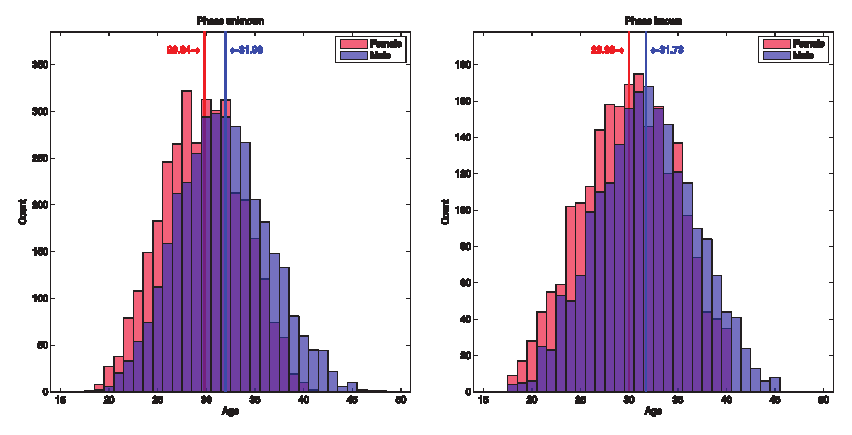
\includegraphics[width=\textwidth]{cointEscape/suppfigs/SupFig-1}
    \vspace{-10pt}
    \captionTitle{\textbf{Age distributions within the filtered dataset.}}{
        The left hand panel shows the distribution for phase-unknown individuals, where the parental ages were averaged across children. 
        The right hand panel shows data for the phase-known meioses where the parental age at the time of childbirth is known.
        Lines indicate the mean of each distribution. 
        Note that some families were excluded from analysis by 23andMe on the basis age to protect privacy, as seen from the truncated distribution of maternal ages in the right hand panel.  
       \label{fig:cointFS1}}
\end{figure}

\begin{figure}[p]
    \centering
    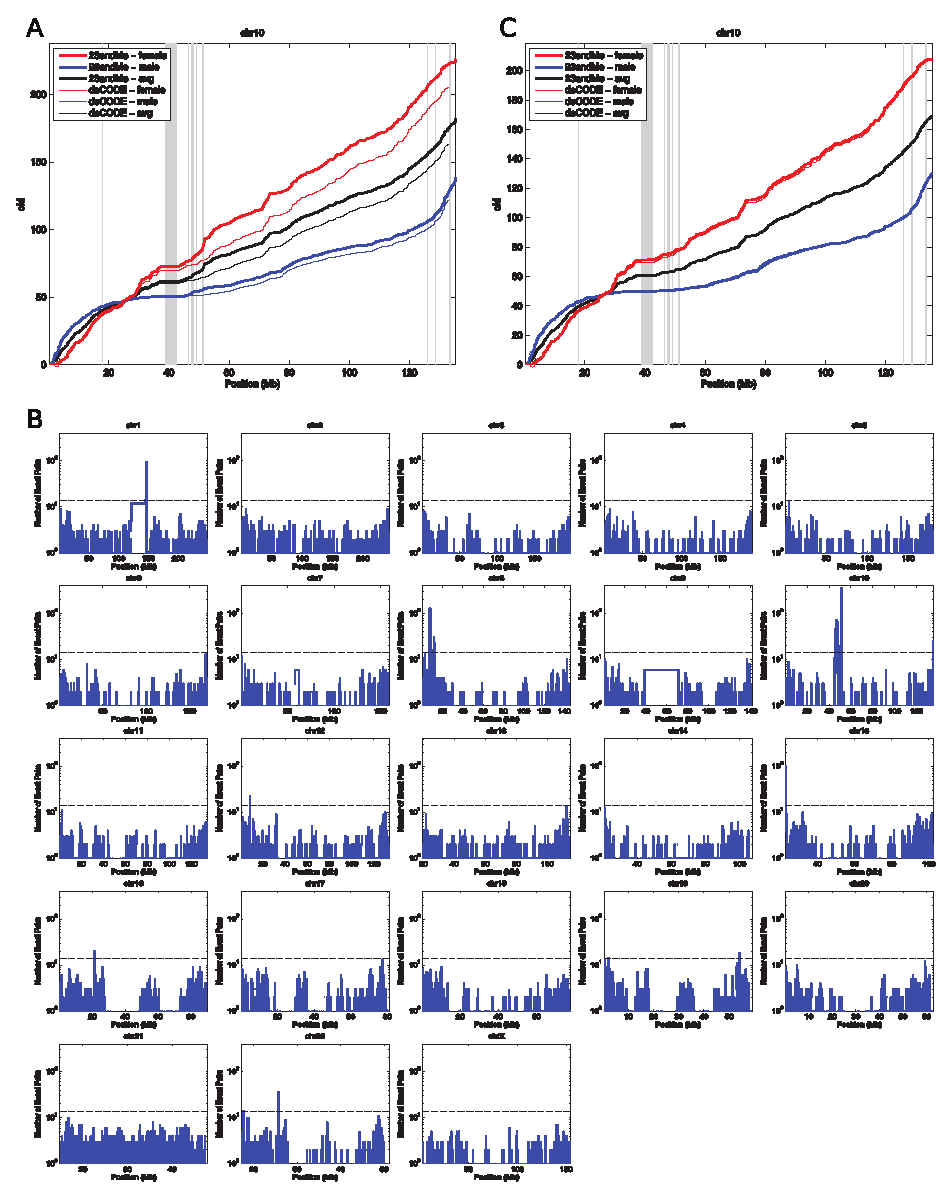
\includegraphics[width=0.9\textwidth]{cointEscape/suppfigs/SupFig-2}
    \vspace{-5pt}
    \captionTitle{\textbf{Data grooming.}}{
        A) Chromosome 10 map before filtering.
        Genetic maps from the 23andMe data are shown in bold lines, whereas the genetic maps from deCODE are shown as thin lines.
        Separate maps are shown for females(red), males (blue), and sex-averaged (black). 
        Also shown are regions highlighted in grey that represent gaps in the reference assembly, the largest of which being the centromere at around 40Mb.
        B) Clustering of recombination events occurring within 1 Mb of each other within single individuals.
        Each plot shows the number of events within 1 Mb of each other on a log$_{10}$ scale as a function of physical position on each chromosome.
        A large number of these event pairs can be observed on chromosome 10, although other large peaks can also be observed on, for example, chromosomes 8 and 15.
        The dashed line represents the 99.9\% percentile of the distribution, and was used as a threshold for filtering.
        C) Chromosome 10 map after filtering.   
       \label{fig:cointFS2}}
\end{figure}

\begin{figure}[!h]
    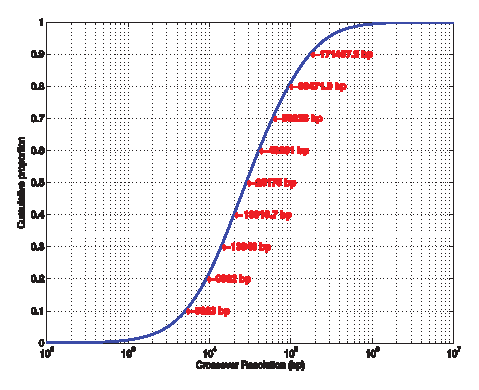
\includegraphics[width=\textwidth]{cointEscape/suppfigs/SupFig-3}
    \vspace{-10pt}
    \captionTitle{\textbf{Empirical cumulative distance function of crossover localization distances.}} { 
        Red labels indicate the interval distances at the distribution deciles.  
       \label{fig:cointFS3}}
\end{figure}

\begin{figure}[!h]
    \includegraphics[width=\textwidth]{cointEscape/suppfigs/SupFig-4}
    \vspace{-10pt}
    \captionTitle{\textbf{Genetic map estimated from 23andMe data.}}{
        Genetic maps from the 23andMe data are shown in bold lines, whereas the genetic maps from deCODE are shown as thin lines.
        Separate maps are shown for females (red), males(blue), and sex-averaged (black).
        Also shown are regions highlighted in grey that represent gaps in the reference assembly. 
        For PAR1, we are showing data derived from Duffy\cite{Duffy2006} for comparison.
        As the deCODE maps cover a slightly smaller physical region than the 23andMe maps, the deCODE maps have been shifted slightly upwards to aid visual comparison.
        Specifically, the deCODE map has been aligned with the 23andMe map at the first physical position within the deCODE map.
        The locations of the alignments are indicated by small circles that can be most clearly seen on the smaller chromosomes.  
       \label{fig:cointFS4}}
\end{figure}

\begin{figure}[!h]
    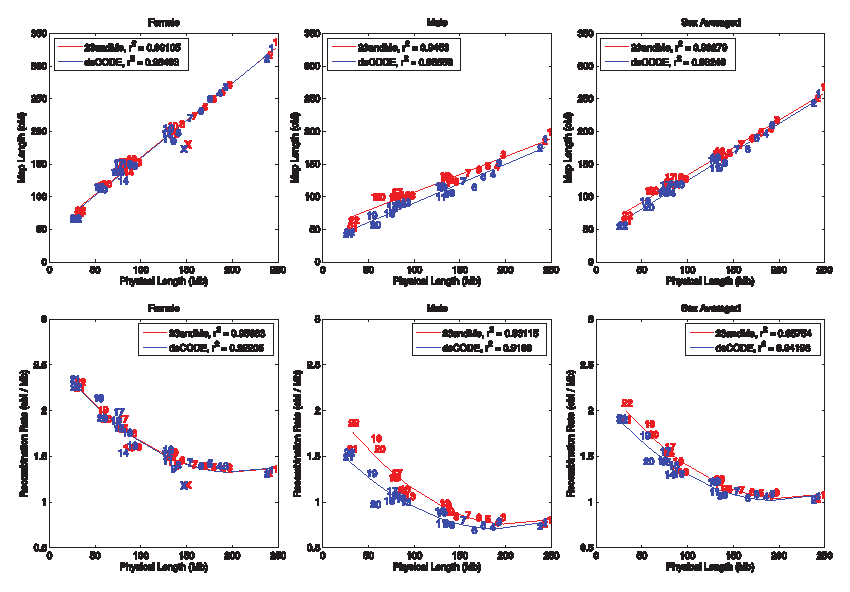
\includegraphics[width=\textwidth]{cointEscape/suppfigs/SupFig-5}
    \vspace{-10pt}
    \captionTitle{\textbf{The relationship between chromosome length and recombination.}}{ 
        The top row shows the correlation between physical length and map length for females (left), males (center), and sex averaged (right), with a linear fit included for the 23andMe map (red) and the deCODE map (blue).
        The bottom row shows the relationship between physical length and average recombination rate with a quadratic fit. 
        Note that chromosome X has been included in the female plots, but was excluded from the regressions.  
       \label{fig:cointFS5}}
\end{figure}

\begin{figure}[!h]
    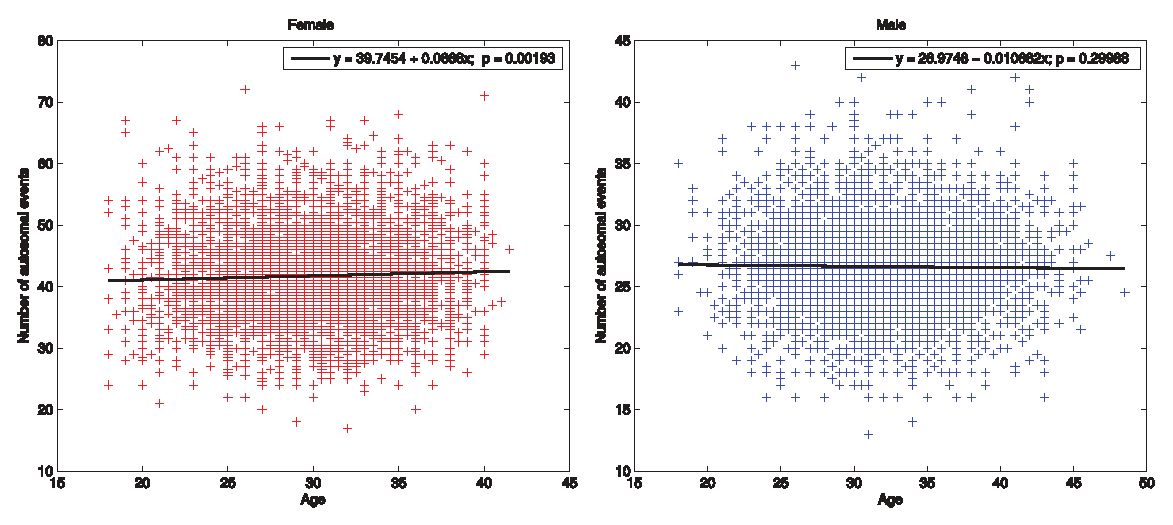
\includegraphics[width=\textwidth]{cointEscape/suppfigs/SupFig-6}
    \vspace{-10pt}
    \captionTitle{\textbf{Number of autosome recombination events versus parental age}}{
        for females (left) and males (right). 
        A linear least-squares fit is indicated by a black line.
        The least-squares fit equation given in the legend together with a p-value for the non-constant term.   
       \label{fig:cointFS6}}
\end{figure}

\begin{figure}[!h]
    \includegraphics[width=\textwidth]{cointEscape/suppfigs/SupFig-7}
    \vspace{-10pt}
    \caption[\textbf{Hotspot usage between sexes.}]{
        A) Hotspot usage estimated in females (left) and males(right). 
        The MLE estimate for each individual is indicated by a circle, with a 95\% confidence interval indicated by the shaded area.
        The median MLE estimate for each sex is indicated by a vertical black line.
        B) Hotspot usage by parental age for females(left) and males (right).
        For each plot a logistic regression is also shown, with the p-value for the non-constant term given in the title.  
       \label{fig:cointFS7}}
\end{figure}

\begin{figure}[!h]
    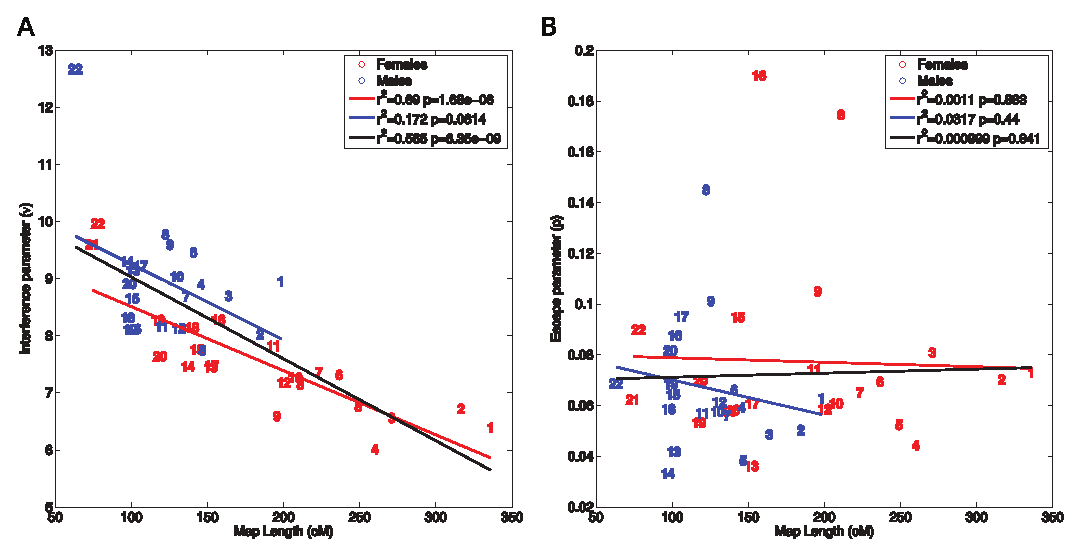
\includegraphics[width=\textwidth]{cointEscape/suppfigs/SupFig-8}
    \vspace{-10pt}
    \caption[\textbf{The relationship between map length and interference parameters.}]{ 
        A) The relationship between chromosome map length and the interference parameter, $\nu$.
        B) The relationship between chromosome map length and the escape parameter, $p$.
        Linear fits are shown for females (red), males (blue), and the data combined across sexes (black).
        In both plots, the chr21 estimate in males has been excluded.  
       \label{fig:cointFS8}}
\end{figure}

\begin{figure}[!h]
    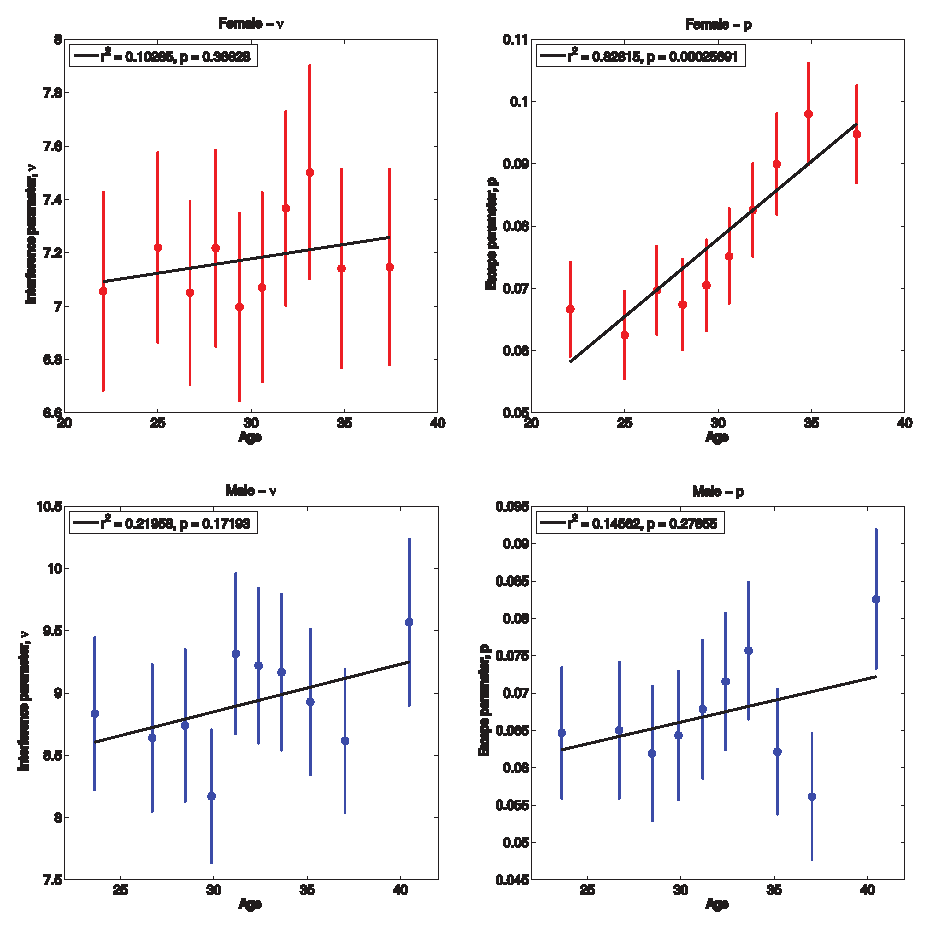
\includegraphics[width=\textwidth]{cointEscape/suppfigs/SupFig-9}
    \vspace{-10pt}
    \captionTitle{\textbf{Interference parameters as a function of age.}}{
        Females and males are shown on the top and bottom rows respectively. 
        Estimates of the interference parameter, $\nu$, are shown on the left, whereas estimates of the escape parameter, $p$, are shown on the right.
        Error bars show 95\% confidence intervals.  
       \label{fig:cointFS9}}
\end{figure}

\begin{figure}[p]
    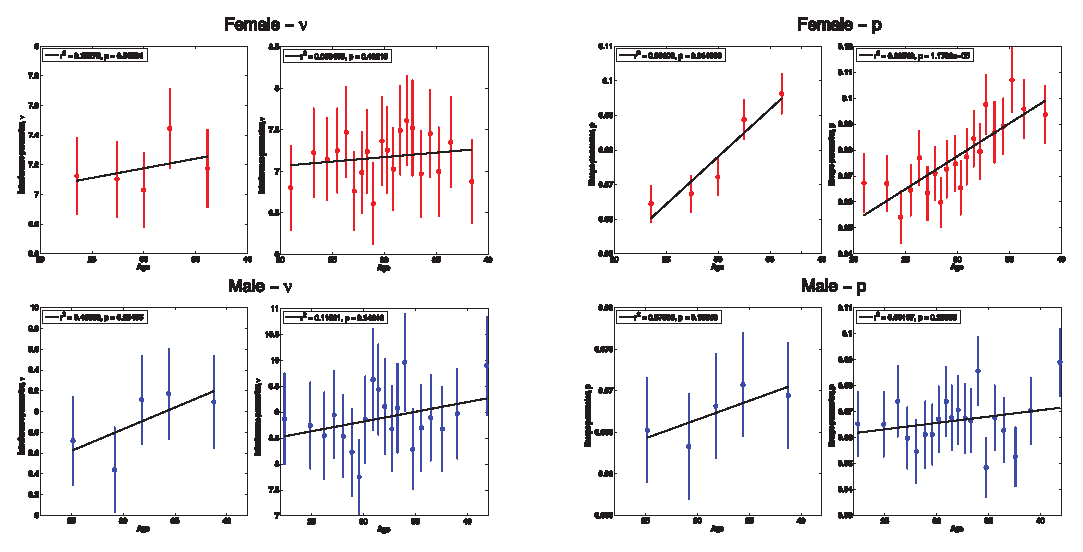
\includegraphics[width=\textwidth]{cointEscape/suppfigs/SupFig-10}
    \vspace{-10pt}
    \captionTitle{\textbf{Interference parameters by age}}{,
        having divided the data in 5 or 20 age quantiles.
        Error bars show 95\% confidence intervals.  
       \label{fig:cointFS10}}
\end{figure}

\begin{figure}[p]
    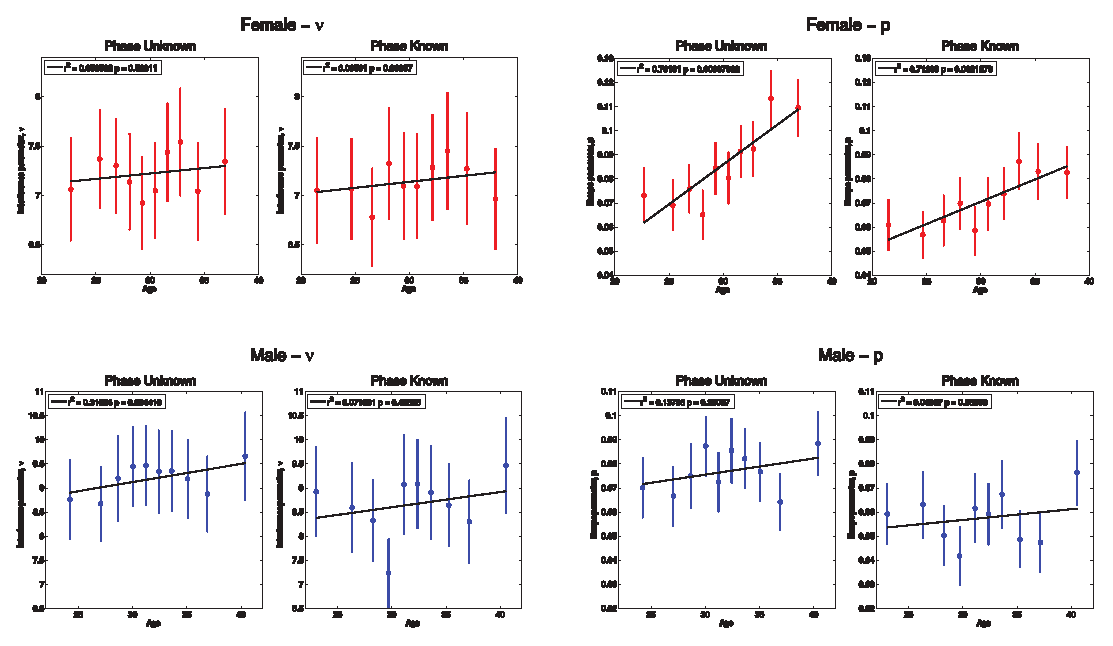
\includegraphics[width=\textwidth]{cointEscape/suppfigs/SupFig-11}
    \vspace{-10pt}
    \captionTitle{\textbf{Interference parameters by age and phase.}}{ 
        Interference parameters by age, having estimated the interference parameters for phase-known and phase-unknown groups separately.  
       \label{fig:cointFS11}}
\end{figure}

\begin{figure}[!h]
    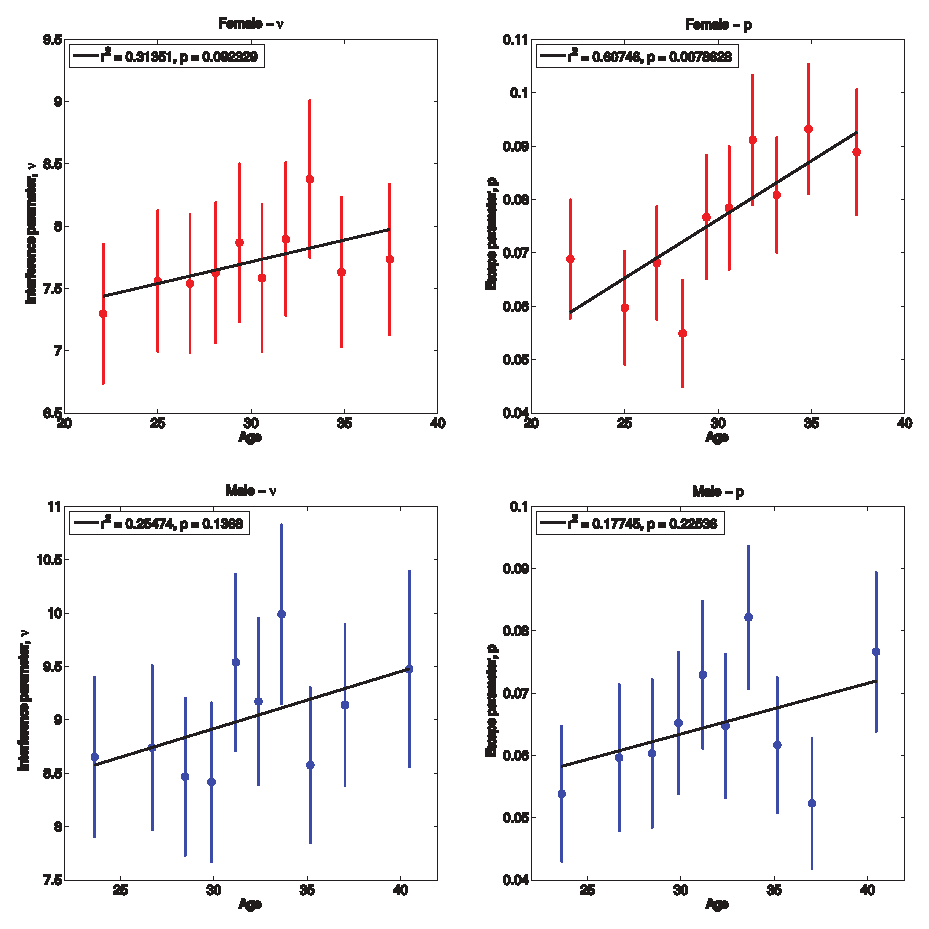
\includegraphics[width=\textwidth]{cointEscape/suppfigs/SupFig-12}
    \vspace{-10pt}
    \captionTitle{\textbf{Interference parameters as a function of age, following stratified sampling.}}{
        Females and males are shown on the top and bottom rows respectively.
        Estimates of the interference parameter, $\nu$, are shown on the left, whereas estimates of the escape parameter, $p$, are shown on the right.
        Error bars show 95\% confidence intervals.  
       \label{fig:cointFS12}}
\end{figure}

\begin{figure}[!h]
    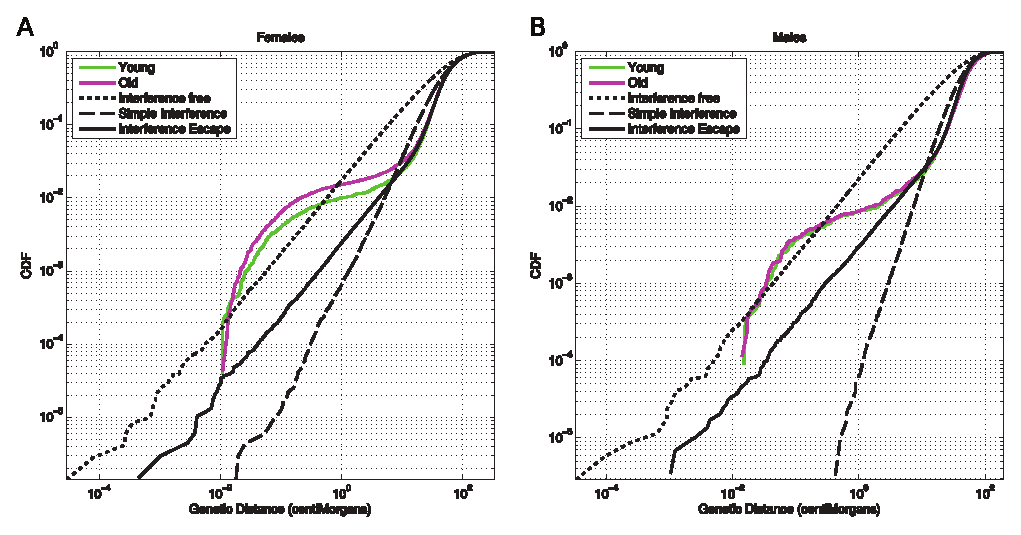
\includegraphics[width=\textwidth]{cointEscape/suppfigs/SupFig-13}
    \vspace{-10pt}
    \captionTitle{\textbf{Model fit for tightly clustered events}}{
        in females (A) and males (B).
        The figure shows the empirical cumulative distribution function for young (green line) and old (magenta line) mothers/fathers, and compares to that obtained via simulation under the interference free model (black dotted line), the Gamma simple interference model (black dashed line), and the Housworth-Stahl interference escape model (solid black line), with parameters were taken from Supplementary Table 7.
        The figure is shown on a log-log scale to emphasize the short inter-crossover distances.  
       \label{fig:cointFS13}}
\end{figure}

\begin{figure}[!h]
    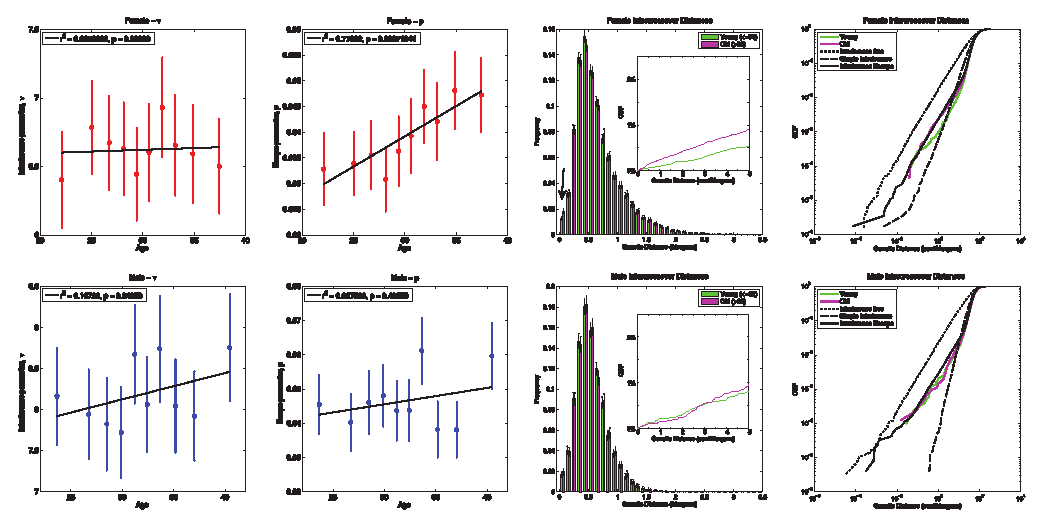
\includegraphics[width=\textwidth]{cointEscape/suppfigs/SupFig-14}
    \vspace{-10pt}
    \captionTitle{\textbf{Interference parameters estimated for a strictly filtered dataset.}}{
        In this case, all crossover events were required at least 10 supporting informative sites (compared to 3 in the main dataset), no two events within a single family were allowed to be within 5 SNPs of each other (compared to 1 in the main dataset), and no more than 4 events within 1 Mb of each other were allowed across the whole dataset (and compared to 14 in the main dataset, which corresponds to the 99.9\textsuperscript{th} percentile).
        After this very strict filtering, the deviation from the Housworth-Stahl interference escape model is much less pronounced at short scales (right hand panels), but the association between interference escape and maternal  
        age remains strong (2\textsuperscript{nd} panel from top left).   
       \label{fig:cointFS14}}
\end{figure}

\clearpage
\section{Supplementary Tables}

\vspace{3cm}
\begin{table}[!h] \centering
    \begin{tabular}{|cccc|} 
        \hline Pedigree Type & Description & Before Filtering & After Filtering \\ \hline
        1 & 2 parents, 2 children & 3319 & 3307 \\
        2 & 2 parents, 3 children & 560 & 523 \\
        3 & 2 parents, 4 children & 89 & 80 \\
        4 & Quartet, with 2nd generation trio & 101 & 100 \\
        5 & Trio, with 2nd generation quartet & 201 & 199 \\
        \hline & \textbf{Total} & \textbf{4270} & \textbf{4209} \\
    \hline \end{tabular}
    \captionTitle{\textbf{Summary of dataset, before and after filtering.}}{
    \label{tab:cointTS1}}
\end{table}

\vspace{3cm}
\begin{table}[!h] \centering
    \begin{tabular}{|p{3cm}p{1.5cm}p{1.5cm}p{1.5cm}p{1.5cm}p{1.5cm}p{1.6cm}|}
        \hline 
    Population & Female \mbox{unphased} & Male \mbox{unphased} & Female phased & Male phased & Total Meioses & Percentage \\ \hline
    Europe & 5382 & 5508 & 1789 & 1641 & 14320 & 78.24\% \\
    Latino & 602 & 546 & 171 & 190 & 1509 & 8.25\% \\
    East Asia & 380 & 308 & 88 & 74 & 850 & 4.64\% \\
    None/Other & 198 & 268 & 68 & 109 & 643 & 3.51\% \\
    South Asia & 178 & 176 & 19 & 20 & 393 & 2.15\% \\
    African American & 152 & 152 & 34 & 36 & 374 & 2.04\% \\
    Middle East & 76 & 100 & 15 & 22 & 213 & 1.16\% \\
    \hline \textbf{Total} & \textbf{6968} & \textbf{7058} & \textbf{2184} & \textbf{2092} & \textbf{18302} & \textbf{100.00\%} \\
    \hline \end{tabular}
    \captionTitle{\textbf{Description of parental ancestry for each meiosis within the sample.}} {
    \label{tab:cointTS2}}
\end{table}

\begin{table}[!h] \centering
    \footnotesize
    \begin{tabular}{|cp{1.0cm}p{1.4cm}p{1.1cm}p{1.1cm}p{1.0cm}p{1.1cm}p{1.0cm}p{1.1cm}p{1.0cm}|}
        \hline 
Chrom & First Position (bp) & Last Position (bp) & Physical Length (Mb) & Female Map Length (cM) & Female Mean Rate (cM/Mb) & Male Map Length (cM) & Male Mean Rate (cM/Mb) & SexAvg Map Length (cM) & SexAvg Mean Rate (cM/Mb) \\ \hline
chr1 & 1,031,540 & 249,170,711 & 248.14 & 335.9 & 1.36 & 198.30 & 0.80 & 267.05 & 1.08 \\
chr2 & 118,913 & 242,763,542 & 242.64 & 316.45 & 1.31 & 184.64 & 0.76 & 250.52 & 1.03 \\
chr3 & 152,592 & 197,759,785 & 197.61 & 270.98 & 1.37 & 163.85 & 0.83 & 217.4 & 1.1 \\
chr4 & 167,596 & 190,787,660 & 190.62 & 260.11 & 1.37 & 145.79 & 0.76 & 202.93 & 1.06 \\
chr5 & 184,702 & 180,673,228 & 180.49 & 249.13 & 1.38 & 146.66 & 0.81 & 197.87 & 1.1 \\
chr6 & 188,937 & 170,777,087 & 170.59 & 236.64 & 1.39 & 140.88 & 0.83 & 188.74 & 1.11 \\
chr7 & 67,365 & 159,042,351 & 158.97 & 223.17 & 1.41 & 136.04 & 0.86 & 179.55 & 1.13 \\
chr8 & 200,898 & 146,235,564 & 146.03 & 210.94 & 1.45 & 122.41 & 0.84 & 166.64 & 1.14 \\
chr9 & 215,269 & 141,004,945 & 140.79 & 195.69 & 1.4 & 125.54 & 0.89 & 160.58 & 1.14 \\
chr10 & 162,102 & 135,402,200 & 135.24 & 207.86 & 1.54 & 129.91 & 0.96 & 168.86 & 1.25 \\
chr11 & 244,552 & 134,872,342 & 134.63 & 193.59 & 1.44 & 120.21 & 0.89 & 156.88 & 1.17 \\
chr12 & 216,039 & 133,684,321 & 133.47 & 200.36 & 1.51 & 131.20 & 0.98 & 165.75 & 1.24 \\
chr13 & 19,458,371 & 114,998,076 & 95.54 & 152.26 & 1.6 & 101.19 & 1.06 & 126.71 & 1.33 \\
chr14 & 20,445,905 & 107,233,999 & 86.79 & 137.22 & 1.59 & 97.29 & 1.12 & 117.24 & 1.35 \\
chr15 & 22,763,396 & 102,381,360 & 79.62 & 143.39 & 1.8 & 100.85 & 1.27 & 122.11 & 1.53 \\
chr16 & 143,503 & 90,102,384 & 89.96 & 157.29 & 1.75 & 102.03 & 1.13 & 129.64 & 1.44 \\
chr17 & 84,782 & 81,025,393 & 80.94 & 152.87 & 1.9 & 106.23 & 1.31 & 129.53 & 1.6 \\
chr18 & 218,695 & 77,955,378 & 77.74 & 140.06 & 1.81 & 97.80 & 1.26 & 118.91 & 1.53 \\
chr19 & 288,246 & 59,058,083 & 58.77 & 117.8 & 2.01 & 99.42 & 1.69 & 108.59 & 1.85 \\
chr20 & 100,699 & 62,892,739 & 62.79 & 118.9 & 1.9 & 99.00 & 1.58 & 108.93 & 1.73 \\
chr21 & 14,807,136 & 47,978,421 & 33.17 & 74.34 & 2.24 & 51.76 & 1.58 & 63.04 & 1.9 \\
chr22 & 17,152,611 & 51,165,664 & 34.01 & 78.16 & 2.31 & 63.30 & 1.86 & 70.71 & 2.08 \\
chrX & 2,737,282 & 154,408,041 & 151.67 & 179.02 & 1.18 &  &  &  &  \\
PAR1 & 178,624 & 2,689,575 & 2.51 & 2.73 & 1.16 & 42.94 & 17.17 & 22.75 & 9.06 \\
PAR2 & 154,984,651 & 155,227,607 & 0.24 & 0.05 & 0.34 & 0.33 & 1.35 & 0.19 & 0.79 \\
        \hline \textbf{Genome} &&& \textbf{2932.98} & \textbf{4354.91} & \textbf{1.48} & \textbf{2707.55} & \textbf{0.92} & \textbf{3441.11} & \textbf{1.17} \\
    \hline \end{tabular}
    \captionTitle{\textbf{Properties of the map estimated from 23andMe data.}}{
        Recombination fractions were converted to genetic map distances using the Haldane map function.  
    \label{tab:cointTS3}}
\end{table}

\begin{table}[!h] \centering
    \footnotesize
    \begin{tabular}{|cccccccc|}
        \hline 
SNP & Chrom & Position & Alleles & P-value & Effect & 95\% CI & Gene Context \\ \hline
rs2001572 & chr14 & 20,767,868 & A/T & 1.50E-08 & 0.503 & [0.329,0.677] & [TTC5] \\
rs79621814 & chr4 & 1,089,268 & C/T & 2.90E-08 & -0.99 & [-1.340,-0.640] & [RNF212] \\
rs11624006 & chr14 & 91,961,188 & C/T & 2.80E-07 & -0.478 & [-0.660,-0.296] & [SMEK1] \\
rs72631326 & chr17 & 65,769,087 & C/T & 4.40E-07 & 0.959 & [0.587,1.331] & NOL11--[]--BPTF \\
rs11932663 & chr4 & 184,458,083 & A/G & 5.10E-07 & 0.622 & [0.380,0.865] & ING2--[]---RWDD4 \\
rs17127442 & chr8 & 18,779,787 & C/T & 5.10E-07 & -0.537 & [-0.746,-0.327] & [PSD3] \\
rs1879904 & chr11 & 82,076,387 & C/T & 6.80E-07 & -0.507 & [-0.707,-0.307] & []---FAM181B \\
    \hline \end{tabular}
    \captionTitle{\textbf{Variants associated with total number of recombination events.}}{
        Linear regression model tested as N\_events $\sim$ sex + age + pc.0 + pc.1 + pc.2 + pc.3 + pc.4 + genotype. 
        Association tests conducted using only individuals found to have $\ge$ 97\% European ancestry. 
    \label{tab:cointTS4}}
\end{table}

\clearpage 

\mbox{} \vspace{3cm}
\begin{table}[h] \centering
    \footnotesize
    \begin{tabular}{|cccccccc|}
        \hline 
SNP & Chrom & Position & Alleles & P-value & Effect & 95\% CI & Gene Context \\ \hline
rs73742307 & chr5 & 23,534,421 & C/T & 7.90E-184 & 0.16 & [0.149,0.170] & PRDM9-[]---CDH10 \\
rs78474856 & chr20 & 1,450,623 & C/G & 6.10E-07 & -0.021 & [-0.029,-0.013] & NSFL1C-[]-SIRPB2 \\
rs62078596 & chr17 & 53,906,496 & C/T & 8.50E-07 & 0.013 & [0.008,0.018] & PCTP--[]---ANKFN1 \\
rs8134126 & chr21 & 28,401,705 & C/T & 1.00E-06 & -0.01 & [-0.013,-0.006] & ADAMTS5--[] \\
rs138108783 & chr1 & 119,711,419 & A/G & 1.40E-06 & 0.274 & [0.163,0.385] & WARS2--[]---HAO2 \\
    \hline \end{tabular}
    \captionTitle{\textbf{Variants associated with hotspot usage.}}{
        Linear regression model tested as hotspot\_usage $\sim$ sex + age + pc.0 + pc.1 + pc.2 + pc.3 + pc.4 + genotype.
        Association tests conducted using only individuals found to have $\ge$ 97\% European ancestry.  
    \label{tab:cointTS5}}
\end{table}

\vspace{2cm}
\begin{table}[!h] \centering
    %\footnotesize
    \begin{tabular}{|cp{1.5cm}p{1.5cm}p{1.5cm}p{1.5cm}cp{2cm}|}
        \hline 
        Population & Female sample size* & Male sample size* & Female median hotspot usage & Male median hotspot usage & Difference & p-value (Mann-Whitney U) \\ \hline
        Europe & 3329 & 3325 & 62.96\% & 67.12\% & 4.16\% & 4.93E-40 \\
        Latino & 362 & 341 & 61.15\% & 66.84\% & 5.68\% & 1.36E-09 \\
        East Asia & 221 & 180 & 60.38\% & 67.56\% & 7.18\% & 5.67E-06 \\
        South Asia & 97 & 95 & 61.65\% & 66.35\% & 4.71\% & 0.00494563 \\
        Middle East & 88 & 88 & 59.52\% & 61.26\% & 1.74\% & 0.284789 \\
        African American & 43 & 57 & 61.37\% & 65.37\% & 4.00\% & 0.135323 \\
        \hline All & 5668 & 5621 & 0.6268 & 0.67255 & 0.04575 & 1.06E-69 \\
    \hline \end{tabular}
\captionTitle{\textbf{Differences in hotspot usage between males and females}}{, partitioned by population.
        *The sample size represents the number estimated $\alpha$s, with one estimate for each meiosis from phase-known parents, and a single estimate for phase-unknown parents.  
    \label{tab:cointTS6}}
\end{table}

\clearpage 
\begin{table}[!h] \centering
    \scriptsize
    \begin{tabular}{|c|p{1.1cm}p{1.2cm}p{1.3cm}|cccccc|} \hline 
    \multicolumn{10}{|l|}{\textbf{Females}} \\ \hline
    & \multicolumn{3}{c|}{\textbf{Gamma model (no escape)}} & \multicolumn{6}{c|}{\textbf{Escape model}} \\
    & Phase known & Phase \mbox{unknown} & Weighted mean & 
    \multicolumn{2}{c}{Phase known} & \multicolumn{2}{c}{Phase unknown} & \multicolumn{2}{c|}{Weighted mean} \\
    Chrom & $\nu$ & $\nu$ & $\nu$ & $\nu$ & p & $\nu$ & p & $\nu$ & p \\ \hline
    chr1 & 2.749 & 3.211 & 2.952 & 6.045 & 0.067 & 6.711 & 0.079 & 6.384 & 0.073 \\
    chr2 & 2.390 & 3.035 & 2.643 & 6.499 & 0.064 & 6.902 & 0.076 & 6.718 & 0.070 \\
    chr3 & 2.328 & 2.653 & 2.473 & 6.489 & 0.072 & 6.612 & 0.089 & 6.556 & 0.081 \\
    chr4 & 3.074 & 3.956 & 3.414 & 5.981 & 0.042 & 6.036 & 0.047 & 6.009 & 0.044 \\
    chr5 & 3.289 & 3.824 & 3.526 & 6.582 & 0.044 & 6.941 & 0.065 & 6.753 & 0.052 \\
    chr6 & 2.893 & 2.864 & 2.878 & 7.221 & 0.055 & 7.395 & 0.086 & 7.314 & 0.069 \\
    chr7 & 3.007 & 2.826 & 2.902 & 7.435 & 0.048 & 7.289 & 0.090 & 7.360 & 0.065 \\
    chr8 & 1.395 & 2.014 & 1.566 & 8.073 & 0.165 & 6.615 & 0.184 & 7.141 & 0.175 \\
    chr9 & 1.760 & 2.590 & 2.007 & 6.168 & 0.095 & 7.096 & 0.113 & 6.586 & 0.105 \\
    chr10 & 2.548 & 4.228 & 2.971 & 7.561 & 0.066 & 7.039 & 0.056 & 7.260 & 0.061 \\
    chr11 & 2.485 & 2.829 & 2.645 & 7.466 & 0.065 & 8.240 & 0.084 & 7.818 & 0.074 \\
    chr12 & 2.979 & 3.896 & 3.323 & 7.519 & 0.058 & 6.927 & 0.060 & 7.175 & 0.059 \\
    chr13 & 3.506 & 4.727 & 3.982 & 7.876 & 0.039 & 7.157 & 0.034 & 7.442 & 0.036 \\
    chr14 & 2.654 & 4.065 & 3.070 & 7.574 & 0.056 & 7.338 & 0.059 & 7.451 & 0.057 \\
    chr15 & 2.090 & 2.604 & 2.292 & 7.652 & 0.081 & 7.842 & 0.109 & 7.754 & 0.095 \\
    chr16 & 1.357 & 1.888 & 1.504 & 7.708 & 0.158 & 9.383 & 0.220 & 8.277 & 0.190 \\
    chr17 & 2.874 & 4.016 & 3.246 & 8.216 & 0.064 & 6.972 & 0.056 & 7.479 & 0.061 \\
    chr18 & 3.063 & 4.920 & 3.575 & 8.244 & 0.064 & 8.056 & 0.053 & 8.139 & 0.058 \\
    chr19 & 3.444 & 5.322 & 4.001 & 7.991 & 0.052 & 8.576 & 0.055 & 8.273 & 0.053 \\
    chr20 & 3.149 & 3.530 & 3.329 & 7.672 & 0.060 & 7.612 & 0.078 & 7.637 & 0.070 \\
    chr21 & 2.694 & 3.596 & 2.996 & 9.454 & 0.061 & 9.713 & 0.064 & 9.598 & 0.062 \\
    chr22 & 2.315 & 1.904 & 2.033 & 9.456 & 0.060 & 10.664 & 0.128 & 9.958 & 0.090 \\
    chrX & 1.959 & 2.151 & 2.050 & 6.439 & 0.089 & 5.886 & 0.110 & 6.129 & 0.100 \\
    Autosomes & 2.409 & 3.084 & 2.666 & 7.134 & 0.071 & 7.233 & 0.086 & 7.188 & 0.078 \\
    \hline\hline
    \multicolumn{10}{|l|}{\textbf{Males}} \\ \hline
    & \multicolumn{3}{c|}{\textbf{Gamma model (no escape)}} & \multicolumn{6}{c|}{\textbf{Escape model}} \\
    & Phase known & Phase \mbox{unknown} & Weighted mean & 
    \multicolumn{2}{c}{Phase known} & \multicolumn{2}{c}{Phase unknown} & \multicolumn{2}{c|}{Weighted mean} \\
    Chrom & $\nu$ & $\nu$ & $\nu$ & $\nu$ & p & $\nu$ & p & $\nu$ & p \\ \hline
    chr1 & 3.240 & 3.289 & 3.266 & 8.515 & 0.047 & 9.419 & 0.082 & 8.949 & 0.063 \\
    chr2 & 4.081 & 3.972 & 4.019 & 7.567 & 0.038 & 8.439 & 0.063 & 8.024 & 0.050 \\
    chr3 & 3.640 & 4.381 & 3.977 & 9.123 & 0.045 & 8.376 & 0.053 & 8.695 & 0.049 \\
    chr4 & 4.469 & 4.256 & 4.343 & 8.516 & 0.046 & 9.217 & 0.072 & 8.895 & 0.059 \\
    chr5 & 4.425 & 5.232 & 4.795 & 7.593 & 0.030 & 7.847 & 0.047 & 7.737 & 0.038 \\
    chr6 & 3.255 & 3.388 & 3.324 & 9.828 & 0.055 & 9.199 & 0.077 & 9.456 & 0.066 \\
    chr7 & 3.266 & 5.311 & 3.873 & 8.297 & 0.057 & 8.991 & 0.055 & 8.685 & 0.056 \\
    chr8 & 2.197 & 1.816 & 1.946 & 10.760 & 0.119 & 9.216 & 0.173 & 9.775 & 0.145 \\
    chr9 & 2.137 & 3.642 & 2.490 & 9.253 & 0.108 & 9.845 & 0.096 & 9.587 & 0.101 \\
    chr10 & 4.323 & 4.823 & 4.564 & 8.575 & 0.047 & 9.556 & 0.071 & 9.031 & 0.058 \\
    chr11 & 3.693 & 4.879 & 4.160 & 7.422 & 0.055 & 8.794 & 0.058 & 8.158 & 0.057 \\
    chr12 & 3.228 & 4.430 & 3.666 & 8.269 & 0.060 & 8.025 & 0.063 & 8.126 & 0.061 \\
    chr13 & 5.706 & 4.058 & 4.467 & 8.387 & 0.029 & 10.051 & 0.058 & 9.142 & 0.042 \\
    chr14 & 4.647 & 5.348 & 4.969 & 9.479 & 0.028 & 9.083 & 0.042 & 9.295 & 0.033 \\
    chr15 & 2.579 & 3.596 & 2.932 & 8.127 & 0.065 & 9.244 & 0.064 & 8.652 & 0.064 \\
    chr16 & 3.485 & 2.641 & 2.875 & 7.675 & 0.064 & 8.492 & 0.105 & 8.114 & 0.088 \\
    chr17 & 3.278 & 2.092 & 2.339 & 8.735 & 0.063 & 9.582 & 0.125 & 9.220 & 0.095 \\
    chr18 & 4.587 & 3.191 & 3.538 & 8.380 & 0.050 & 8.278 & 0.066 & 8.314 & 0.058 \\
    chr19 & 3.808 & 4.607 & 4.156 & 7.423 & 0.061 & 8.975 & 0.074 & 8.104 & 0.068 \\
    chr20 & 3.184 & 3.478 & 3.333 & 8.205 & 0.079 & 9.601 & 0.084 & 8.905 & 0.082 \\
    chr21 & 2.485 & 5.772 & 2.841 & 100 & 0.074 & 100 & 0.049 & 100 & 0.057 \\
    chr22 & 2.467 & 3.414 & 2.786 & 10.442 & 0.059 & 16.799 & 0.074 & 12.670 & 0.069 \\
    Autosomes & 3.346 & 3.591 & 3.470 & 8.608 & 0.058 & 9.184 & 0.077 & 8.931 & 0.067 \\
    \hline \end{tabular}
    \captionTitle{\textbf{Interference parameter estimates for females (top) and males (bottom).}}{
        Estimates are given for phase-known and phase-unknown individuals separately.
        In addition, a combined estimate was calculated as a weighted average with weights taken to be the reciprocal of the variance.  
    \label{tab:cointTS7}}
\end{table}

\begin{table}[!h] \centering
    \small
    \begin{tabular}{|ccc|}
\hline Chrom & Start position (bp) & End position (bp) \\ \hline
1 & 144,954,851 & 145,394,955 \\
1 & 145,547,963 & 146,508,934 \\
1 & 146,997,245 & 147,093,887 \\
1 & 147,162,445 & 147,205,770 \\
1 & 147,210,993 & 147,222,372 \\
1 & 147,375,981 & 147,782,284 \\
8 & 6,881,638 & 8,119,716 \\
8 & 11,088,131 & 11,096,553 \\
8 & 11,251,705 & 11,256,184 \\
8 & 11,330,364 & 11,332,026 \\
8 & 11,354,933 & 11,359,638 \\
8 & 11,363,950 & 11,372,141 \\
8 & 11,406,175 & 11,476,726 \\
8 & 11,486,220 & 11,496,193 \\
8 & 11,501,265 & 11,503,333 \\
8 & 11,514,144 & 11,516,373 \\
8 & 11,533,384 & 11,570,036 \\
8 & 11,722,125 & 11,755,513 \\
8 & 11,763,932 & 11,799,654 \\
8 & 11,830,877 & 11,846,482 \\
8 & 11,857,317 & 12,559,475 \\
10 & 46,076,235 & 47,597,927 \\
10 & 47,611,631 & 48,324,245 \\
10 & 48,368,273 & 48,380,952 \\
10 & 48,400,458 & 48,427,246 \\
10 & 48,440,744 & 48,471,020 \\
10 & 48,489,541 & 48,508,137 \\
10 & 48,512,114 & 48,545,527 \\
10 & 50,122,109 & 50,163,975 \\
10 & 50,382,038 & 50,382,478 \\
10 & 50,451,843 & 50,471,176 \\
10 & 50,568,814 & 50,585,177 \\
10 & 50,615,087 & 50,615,806 \\
10 & 50,623,895 & 50,643,498 \\
10 & 50,821,243 & 50,824,244 \\
10 & 50,824,619 & 51,559,469 \\
10 & 135,160,950 & 135,195,332 \\
10 & 135,202,594 & 135,257,091 \\
10 & 135,347,727 & 135,349,367 \\
10 & 135,351,362 & 135,352,100 \\
12 & 8,000,912 & 8,021,932 \\
15 & 22,876,889 & 22,908,392 \\
15 & 22,909,207 & 22,918,657 \\
15 & 22,932,511 & 23,053,839 \\
16 & 21,327,273 & 21,620,270 \\
19 & 2,098,015 & 2,099,820 \\
19 & 54,077,870 & 54,106,839 \\
19 & 54,107,686 & 54,111,568 \\
22 & 17,729,044 & 17,731,977 \\
22 & 25,650,406 & 25,848,811 \\
    \hline \end{tabular}
    \captionTitle{\textbf{Locations of regions with high numbers of double recombination events.}} {
            Hg19 coordinates.  
    \label{tab:cointTS8}}
\end{table}

\clearpage

\section{Supplementary Methods}

\subsection{Assessment of robustness to genotyping error}

In order to understand how our results could be influenced by genotyping  
error we simulated data for each of the pedigree structures contained within our  
data.  To do this, we generated haplotypes for the founder individuals using the  
coalescent simulation software ms\cite{Hudson2002}.  Specifically, we generated 6 haplotypes (using:  
\verb|ms 6 1 -t 2189.781|) and combined haplotypes at random to generate the genotypes  
of the founders.  The population mutation rate was selected give an expected  
number of 5000 segregating sites. Children were then created by drawing  
haplotypes from each parent, and adding recombination as required.   

To test MERLIN's ability to detect crossover events we placed one  
recombination event in the center of the sequence in one random parent, and  
passed this simulated pedigree data to MERLIN for haplotype analysis (option
\verb|--best|).  This process is repeated to obtain 1000 total events per parent in each  
pedigree structure. Our results indicate that MERLIN is able to capture 99.6\% of  
recombination events generated in this manner. The false negative calls resulted  
from low levels of heterozygosity (i.e. high relatedness) in the simulated haplotypes.  
The events placed in phase-known pedigrees were correctly assigned to the proper  
child in all cases. We repeated this simulation in the absence of any introduced  
recombination and find that in all cases, no events were called.  

Estimates of the error rate of the Illumina HumanOmniExpress array used by  
23andMe range from 0.01\%\cite{Illumina2013}  to 0.054\%\cite{Imai2010}.  To test for robustness of our results to  
genotyping error, we next simulated pedigrees without recombination, but with a  
single genotyping error introduced into one of the individuals by switching one of  
the alleles at the middle site in the sequence.  This procedure was repeated 1000  
times in each of the five pedigree structures in our dataset.  We looked for any  
events called by MERLIN and recorded the position in the sequence and the number  
of informative sites to the left and right of the event.    

We estimated the number of false recombination events as a function of  
genotyping error.  Without any filtering (and without using MERLIN's error  
detection functionality), we find MERLIN to be sensitive to genotyping error. For a  
dataset of our size and pedigree composition, a genotyping error rate of 0.001\%  
would produce 15,000 false positive recombination events, rising to 150,000 for a  
0.01\% genotyping error rate. However, the filters applied in the real dataset are  
effective at removing these simple false positives. After requiring at least 3  
informative sites on both sides of a recombination event, we estimate that a dataset  
of our size would contain 74 spurious events with a 0.001\% genotyping error rate,  
739 with a 0.01\% genotyping error rate, and 7,386 with a 0.1\% genotyping error  
rate.   

Although the assumptions of this simulation study are quite simplistic, given  
our dataset contains over 645,000 events these results would suggest that less than  
1\% of the events represent false positives. In addition, we note that in analysis of  
the real data, we used high-confidence sites and removed potential
genotyping errors using MERLIN's error-detection feature (see Methods).  

\subsection{Individual Ancestral Assignment}
 
Individuals were assigned to ancestral categories by quantifying the
genetic variation they share with a set of representative reference
populations.Chromosomal segments are assigned to geographic regions using
23andMe's Ancestry Composition tool\cite{23andMe2014}.  Informally, Ancestry Composition assigns
regions of an individual's genome to 31 reference populations constructed from
public reference datasets as well as private 23andMe cohort data\cite{23andMe2012}.  
Individuals are assigned to genomic regions by first splitting the genome into short
non-overlapping segments, and assigning each segment to the reference
population with the highest degree of similarity. Given this assignment, it is
straightforward to compute the percentage of an individual's DNA that originates
from a certain sub-population.  For example, if 200,000 out of 400,000 total
segments are predicted to come from an African background, then the global
percentage of African ancestry is 50\%.  Given this global percentage,
individuals are assigned to high-level categories (European, Middle Eastern,
East Asian or South Asian) if their total percentage of ancestry in
that category exceeds 97\%. For individuals of admixed ancestry, 23andMe uses a
logistic classifier trained on the segment length distributions of individuals
who have self-identified as African American or Latino. In order to
define the final population label for a given individual, we first determined if
they had at least 97\% European, Middle Eastern, East Asian or South Asian
ancestry. If so, then their category was determined.  If the 97\% threshold
was not met, but the individual had a total global percentage of at least 97\%
when summing contributions from European, African and Native American, then
the logistic classifier was applied. If neither of these conditions were met,
then the individual was categorized as ``Other''.  
 
\subsection{Estimation of hotspot usage }
 
To estimate the degree of hotspot usage by an individual, we adopted the  
method of Coop et al.\cite{Coop2008}. In brief, this method estimates the fraction of recombination  
events that overlap with known LD-based hotspots while accounting for the  
uncertainty in the localization of the called recombination events. For convenience,  
we re-describe the approach here.  
 
We aim to estimate the proportion, $\alpha$, of events that occur within LD-based  
hotspots. Given a recombination event, $r$, the probability that the event overlaps  
with a hotspot is given by:  
\[
    P ( r \text{ overlaps a hotspot} ) = \alpha + (1-\alpha) P(r \text{ overlaps a hotspot by chance} )
\]
To estimate $P(r \text{ overlaps a hotspot by chance})$, we randomly shift the  
recombination events by a normally distributed distance (mean 0, standard  
deviation 200kb) a total of 1,000 times, and calculated the fraction of these moves  
that result in the event overlapping a hotspot. The likelihood for $\alpha$ is given by:  
\[
    L(\alpha|r) = \delta_r P( r \text{ overlaps a hotspot} ) + (1 - \delta_r)( 1 - P( r \text{ overlaps a hotspot}) )
\]
where $\delta_r$ is an indicator function, taking the value 1 if $r$ overlaps a hotspot and zero  
otherwise. For a set of $k$ recombination events labeled $r_0,r_1,\dots,r_{k-1}$, the likelihood  
of $\alpha$ for the whole dataset is given by:  
\begin{equation}
    L(\alpha|r_0,r_1,\dots,r_{k-1} = \prod_{i=0}^{k-1} L(\alpha|r_i) .
\end{equation}

We used this method to estimate $\alpha$ for each mother and father (for phase
unknown individuals), and each meiosis (for phase known individuals). As in \citet{Coop2008},
we used all events that were well localized to within 30kb, but note that our  
results are robust to larger values of this parameter. The likelihood of alpha was  
estimated over a uniformly spaced grid of 2,000 values between 0 and 1, with the  
MLE taken as the value of $\alpha$ with the maximum likelihood on this grid. A 95\%  
confidence interval was constructed as being the set of values within two log  
likelihood units of the MLE.    

For phase-known individuals for which recombination events could be  
assigned to specific children, a separate $\alpha$ was estimated for each meiosis. For  
phase-unknown individuals where such an assignment was not possible, $\alpha$ was  
estimated using all events that could be attributed to the parent.  


\subsubsection{Hotspot usage results} % \mbox{}
 
The estimates for hotspot usage are shown in Supplementary Figure \ref{fig:cointFS7}. 
The  median hotspot usage estimate for females was 62.68\% (95\% C.I. 62.25\% - 63.10\%),
whereas for males it was 67.26\% (95\% C.I. 66.85\% - 67.69\%), a difference of 4.6\%  
($p=$ \num{1.1e-69}, Mann-Whitney U).  

To ensure the difference between males and females is not driven by higher  
precision in females (resulting from higher numbers of events), we thinned the  
female data in order to match the number of events in males. Specifically, for each  
male, we randomly selected a female (without replacement) with a greater or equal  
number of events, and thinned the female events to match the number of male  
events. The resulting dataset contains an equal number of males and females, with  
each pair having an equal number of events. The estimates of hotspot usage for the  
two sexes were very similar to the previous estimates (62.2\% for females, and  
66.8\% for males), and the difference in hotspot usage remains highly significant  
($p<$ \num{2.2e-16}).  

To determine whether the observed differences in hotspot usage between  
males and females is dependent on the position within the chromosome (as males  
tend to have higher recombination rates towards the telomeres), we repeated the  
analysis having divided each chromosome into segments. Specifically, we split each  
chromosome into three windows, assigning the terminal 25\% of sequence from  
each end to p- and q-arm bins, and keeping the central 50\% of the sequence for the  
middle bin. For acrocentric chromosomes we omit the p-arm bin. We estimated the  
degree of hotspot usage in each of these bins. We observe that males use hotspots to  
a greater extent than females (Mann-Whitney U $p<$ \num{2.2e-16} for all three bins),  
suggesting that the difference in hotspot usage between males and females
cannot be explained by telomere effects.  

Due to variation in PRDM9, hotspot
usage is expected to vary between populations\cite{Hinch2011,Berg2011}. The hotspots used in this
study were identified from genome-wide Phase II HapMap linkage disequilibrium
data\cite{hapmap2007}, in which hotspots were called that were active in at least two of the
three constituent populations (CEU, YRI, JPT+CHB). As such, one possibility for
the observed difference between males and females is that the ancestry
proportions within our data differ between the female and male samples.
Inspection of the ancestry proportions within our data showed this not to be the
case. In addition, if the analysis is partitioned by inferred ancestry,
females have lower hotspot usage within all populations (Figure \ref{fig:cointF2}B), with the
difference remaining significant in European, East Asian, Latino, and South
Asian populations(Supplementary Table \ref{tab:cointTS6}).  

\subsection{Description of age effect}
 
Previous research has indicated a relationship between maternal age and
the number of recombination events. In particular, research from the
deCODE consortium used data from 14,140 meioses to report that the number
of recombination events in females increase with age\cite{Kong2004}. The reported effect size
is reasonably modest, contributing 0.082 ($\pm$ 0.012 standard error)
recombination events per year, depending on the analysis method used. This
translates as approximately a 4\% increase in the average maternal recombination
rate over a period of 25 years. No such association was observed in males.  A
second study confirmed this effect using 728 meioses observed with
from Hutterite families\cite{Coop2008}, observing that mothers over 35 years of age had
approximately 3.1 extra recombination events compared to those under 25. Despite
the small sample size, the effect size in this study was estimated to be 0.19 
($\pm$ 0.092 standard error) events per year. Again, no such effect was observed in
males.   
 
Conversely, a separate research group considering recombination events in 195
meioses reported a decrease in the number of recombination events with maternal
age\cite{Hussin2011}. In this case, the effect size was larger, corresponding to between 
$-$0.49 and $-$0.42 crossovers per year, again with no such effect observed in
males. Although the smallest of the three studies, the authors suggest that the
discrepancy in the direction of the effect between studies could be due to
marker density and/or true biological differences between populations.

\subsubsection{Correlation between number of recombination events and parental age} % \mbox{}

To quantify the correlation between parental age and recombination rate,
we first partitioned our data into phase-unknown parents for which
recombination events could not be assigned to a specific child (or meiosis), and
phase-known parents for which such an assignment was possible. For the
phase-unknown parents group we used the maternal / paternal ages averaged
across children, whereas for the phase-known group, we used the known parental
ages at the time of the child's birth.

Using linear regression, we estimated the association between the number
of autosomal events and parent age (Supplementary Figure \ref{fig:cointFS6}). 
A weak positive association between age and the number of recombination events was
detected for females, but no such effect was observed for males. The number of
recombination events in females increased on average by 0.067 per year (standard
error: $\pm$ 0.0215), which is similar to the estimate from deCODE.  

We note that the observed effect is quite weak, and appears to be largely
driven by an increase in the number of recombination events for mothers of 35
years or older (Figure \ref{fig:cointF1}C).  

To ensure the observed effect is not confounded by population
structure within the data, we first repeated the analysis for each population
separately. In Europeans, for whom we have by far the largest sample size
(accounting for $\sim$76\%of individuals), a significant association with maternal
age was still observed (0.087 extra events per year, $p=$ \num{3.2e-4}). In all
other populations (East Asian, Middle Eastern, Latino, African American, and
South Asian), no significant association was observed, possibly due to
insufficient power. No significant association with paternal age was observed
within any population.  

\subsection{Inferring Crossover Interference}
In the following text, we provide a description of the crossover interference
models used within the main analysis.  

\subsubsection{The Gamma Model (a.k.a. the `simple interference' model)} % \mbox{}

We follow the description of the Gamma model of crossover interference  
presented by Broman and Weber\cite{Broman2000}. For clarity, we repeat the description of this the  
model below.  

The Gamma model describes the locations of chiasmata on the four-strand  
bundle according to a stationary renewal process, with increments being drawn  
from a gamma distribution with shape $\nu$ and rate 2$\nu$. As such, in this model the  
distances between chiasmata are independent with mean 0.5 Morgans, and a  
standard deviation of $(2 \sqrt{\nu})^{-1}$. Under the assumption of no chromatid interference,  
the chiasmata are thinned such that each chiasmata becomes a crossover with  
probability 0.5. As such, this model satisfies the requirement that the average 
inter-crossover distance should be 1 Morgan.   

The parameter $\nu$ is a unitless measure of the strength of interference.   
Specifically, $\nu$ = 1 corresponds to no interference between chiasmata, and $\nu>$ 1  
corresponds to positive interference (i.e.\ decreased variance in chiasmata spacing  
than would be expected under a Poisson model), and $\nu<$ 1 corresponds to negative  
interference (i.e.\ increased variance in chiasmata spacing than expected under a  
Poisson model).  

Let $x_0,x_1,x_2,\dots$ be the genetic distances (in Morgans) between adjacent  
chiasmata, with $x_0$ being the distance from the p-terminal end of the chromosome to  
the first chiasma. Under the Gamma model, the chiasmata locations are generated  
according to a gamma renewal process, such that $x_1,x_2,\dots$ are independent and  
follow a gamma distribution with shape $\nu$ and rate 2$\nu$, where $\nu$ is a positive real number.
Therefore, the density of $x_i$ is given by $f(x;\nu) = (2\nu)^\nu e^{-2 \nu x} x^{\nu-1} / \Gamma(\nu)$,
for $i>0$, and where $\Gamma(.)$ represents the gamma function. The density of $x_0$ is given by
$g(x;\nu) = 2 [ 1-F(x;\nu) ]$, where $F$ is the cumulative distribution function (cdf) of $f$.  

However, using transmitted genotype data, the actual chiasmata locations are not observed. 
Rather, only the crossovers derived from the chiasmata positions are observed. Assuming 
no chromatid interference, the probability that a chiasmata results in a crossover is $\frac{1}{2}$.


Let $y_0,y_1,y_2,\dots$ be the genetic distances (in Morgans) between adjacent crossovers.  
Each $y_i$ is independent, with density given  by
$f^*(y;\nu) = \sum^\infty_{k=1} (\frac{1}{2})^k f_k(y;\nu)$,
where is the gamma distribution density with shape $k\nu$ and rate $2\nu$:
$f_k(k;\nu) = (2\nu)^{k \nu} e^{-2 \nu x} x^{k \nu -1} / \Gamma(k \nu)$,
which is derived from the convolution of $f(y;\nu)$ with itself $k$ times. 
The density of $y_0$ is given by $g^*(k;\nu) = 1 - F^*(y;\nu)$, where $F^*$  is the cdf of 
$f^*$. Likewise, let $G^*$ represent the cdf of $g^*$.  

Given the above model, the contribution to the likelihood is:   
\begin{equation}
    Lk(\nu;y) = 
    \begin{cases}
        1 - G^*(L;\nu)
        & \text{if $m_i = 0$} \\

        g^*(y_0;\nu) g^*(y_1;\nu)
        & \text{if $m_i = 1$} \\

        \displaystyle g^*(y_0;\nu) \Bigg[ \prod_{j=1}^{m_i-1} f^*(y_j;\nu) \Bigg] g^*(y_m;\nu)
        & \text{otherwise} \\

    \end{cases}
\end{equation}
The likelihood for the complete data may be obtained as the product over all individual contributions.   

\subsubsection{The Housworth-Stahl `interference escape' model.} % \mbox{}
 
The Gamma model assumes that all crossover events are subject to the same
interference process. The model has been shown to fit the data reasonably well for
numerous organisms\cite{Broman2000,Broman2002}. However, evidence from model organisms 
suggests the existence of a subset of events that are not subject to crossover interference\cite{Baudat2007},
and statistical support of this finding has been seen in humans\cite{Fledel-Alon2009,Housworth2003}.  

For this reason, we adopt the Housworth-Stahl model of interference, which models 
the distances between crossovers as being a mixture of two processes. In one process, 
crossovers are distributed according to the gamma model described above, whereas in the
second process, crossovers are distributed without interference. We describe this model here,
following Housworth and Stahl's 2003 paper\cite{Housworth2003}, and refer to it as the 
`interference escape' model.  

Assume that we have a mixture of two independent types of crossover, such that one type 
occurs with probability $q$ and has interference parameter $\nu$, and the other type occurs
with probability $p = 1 - q$ and is not subject to interference ($\nu =$ 1). 
As for the Gamma model described above, let $x_0,x_1,x_2,\dots$ be the genetic distances
(in Morgans) between adjacent chiasmata, with $x_0$ being the distance from the p-terminal
end of the chromosome to the first chiasma. The distances between chiasmata are given
by a gamma distribution with shape $\nu$  and rate $2 q \nu$. As such, the density of
$x_i$ is given by $f(x;\nu,2 q \nu) = (2 q \nu)^\nu e^{-2 q \nu x} x^{\nu-1} / \Gamma(\nu)$,
for $i > 0$. Likewise,
the density of $x_0$ is given by $g(x;\nu,q) = 2q [ 1 - F(x;\nu,2q\nu) ]$, where $F$ is the
cumulative distribution function (cdf) of $f$.  

As described for the Gamma model, crossover events are determined by thinning 
the chiasmata positions, with each position retained with probability $\frac{1}{2}$.
Let $y_0,y_1,y_2,\dots$ be the genetic distances (in Morgans) between adjacent crossovers
of this type. Each $y_i$ is independent, with density given by
$f^*(y;\nu,q) = \sum_{k=1}^\infty (\frac{1}{2})^k f(y;k\nu,2q\nu)$.
The density of $y_0$ is given by $g^*(k;\nu,q) = q [ 1 - F^*(y;\nu,q)]$, where $F^*$ is the cdf of $f^*$.
Likewise, let $G^*$ represent the cdf of $g^*$.  

Now consider a dataset from a single meiosis where the intercrossover distances are given by 
$x_0,x_1,x_2,\dots,x_n$, where $\sum_{i=0}^n x_i = L$. We assume these events are derived from 
two types of crossover. The interference-free type occurs with probability $p$ and has $\nu=$ 1.
The second type is subject to interference and occurs with probability $q = 1 - p$. 
To calculate the likelihood of the data, we must sum over the $2^n$ possible ways to assign 
crossovers to the two types. Given one possible assignment, we split the data into two sets of 
intercrossover distances, $y_0,y_1,y_2,\dots,y_j$ for the interference-free type, 
and $z_0,z_1,z_2,\dots,z_k$ for the second `interference' type, where $j + k = n + 1$.
The likelihood of the data in from the interference-free type is:  
\begin{equation}
    Lk(\nu = 1,q=p;y) =  
    \begin{cases}
        1 - G^*(L;1,p)
        & \text{if $j=0$} \\
        g^*(y_0;1,p) [ 1-F^*(y_1|1,p) ]
        & \text{if $j=1$} \\
        \displaystyle g^*(y_0;1,p) \Bigg[ \prod_{i=1}^{j-1} f^*(y_i;1,p) \Bigg] \Big[ 1-F^*(y_j|1,p) \Big]
        & \text{otherwise.} \\
    \end{cases}
\end{equation}
The likelihood of the data from the interference type is: 
\begin{multline}
    Lk(\nu = t,q=1-p;z) = \\
    \begin{cases}
        1 - G^*(L;t,1-p)
        & \text{if $j=0$} \\
        g^*(y_0;t,1-p) [ 1-F^*(y_1|t,1-p) ]
        & \text{if $j=1$} \\
        \displaystyle g^*(y_0;t,1-p) \Bigg[ \prod_{i=1}^{j-1} f^*(y_i;t,1-p) \Bigg] \Big[ 1-F^*(y_j|t,1-p) \Big]
        & \text{otherwise.} \\
    \end{cases}
\end{multline}
To calculate the likelihood of the data, we sum over all $2^n$ possible assignments to the two types:  
\begin{multline}
    Lk'(\nu=t,q=p;x) =
    \sum_{\substack{ (y_0,y_1,y_2,\dots,y_j),\\
                     (z_0,z_1,z_2,\dots,z_k) 
             }} Lk(\nu=1,q=p;y) Lk(\nu=t,q=1-p;z)
\end{multline}
To calculate the likelihood over multiple individuals, one simply takes the product of the above likelihood.  

In our implementation of the above formulas, we calculated $f^*$ by summing over $k$ from 0 to 25. 
Numerical integration was used to calculate $G^*$ using the \textit{integral} function in MATLAB.   

\subsubsection{Extension to interference escape model for phase-unknown data} % \mbox{}
 
The above description of the interference escape model assumes that the observed crossover
events can be assigned to a specific meiosis. However, in the case of the phase-unknown
individuals that make up the majority of our data, the observed crossovers cannot be 
assigned to specific children. As such, the above model cannot be used.  

To extend the model for phase-unknown, we perform the same trick of summing over all 
possible assignments to each type, but this time also summing over all possible assignments
to each meiosis. Although this procedure is somewhat na\"{i}ve, both simulations and 
comparison of results between phased and unphased families have shown that it works well
in practice (Supplementary Figure \ref{fig:cointFS11}).   

Consider a family quartet. For each parent, the observed crossovers are the result of 
two independent meioses, which we will call $M_1$ and $M_2$ respectively. Let the intercrossover
distances events in $M_1$ be $a_{i0},a_{i1},a_{i2},\dots,$ and the intercrossover distances in 
$M_2$ be $b_{i0},b_{i1},b_{i2},\dots,$ where $a_{i0}$ and $b_{i0}$ represent the distances between
the first event and the p-terminal end of the chromosome in $M_1$ and $M_2$ respectively.
If we could observe these intercrossover distances, we could apply the Housworth-Stahl 
model as described above. However, due to the nature of phase-unknown individuals, all
we are unable to directly observe these distances, and can only observe crossovers derived 
from both meioses without knowing which event is from which meiosis.  

Na\"{i}vely, we could be to sum over all possible assignments to each meiosis,and for each
assignment apply the Housworth-Stahl model independently. However, this would be inefficient,
as it would result in summing over $4^n$ possible assignments (as there are 2 crossover types 
in each of 2 meioses). Instead, we note that the same result can be achieved by combining the
`interference free' classes, allowing us to sum over $3^n$ possible assignments. 
   
Let the $n$ observed crossover positions assigned to a parent be $z_{i1},z_{i2},z_{i3},\dots,z_{in},$ 
which are derived from a superposition of the gamma renewal processes. In order to calculate the 
likelihood of this data, we treat the assignment of each event as either belonging to one of 
two inference classes, or to a single interference free class. Specifically, we calculate the likelihood as:  
\begin{multline}
    Lk'(\nu,q;z) = \\
    \sum_{\substack{ (a_0,a_1,\dots,a_i), \\
                     (b_0,b_1,\dots,b_i), \\
                     (c_0,c_1,\dots,c_i)
             }}
    \Big[ Lk(\nu=t,q=1-p;a) Lk(\nu=t,q=1-p;b) Lk(\nu=1,q=2p;b) \Big]
\end{multline}
where the summation is taken over all possible $3^n$ divisions of the $n$ crossovers into  
the three classes. The likelihood for the complete dataset is given by taking the  
product of $Lk'(\nu,q;z)$ over all individuals. 

Maximum likelihood estimation of $\nu$ and $q$ was performed using a MATLAB  
implementation of the Nelder-Mead method\cite{DErrico}, restricting the search space such  
that $\nu \in [0.1,100]$, and $q \in (0,0.5)$. Uncertainty in the MLE point estimates was  
obtained by using the inverse of the Fisher information matrix to estimate the  
covariance matrix.  
 
We note that the mixture model lacks identifiability when $\nu$ is close to 1. 
In this situation, the estimates of $q$  become uninformative. When performing likelihood 
maximization, we experimented with including a weakly informative prior on $q$  that favors 
smaller values. Specifically, we set $P(q)= 1 - q$, and performing maximum a posteriori 
estimation in place of maximum likelihood. In simulations, we found this method slightly 
improved results when $\nu$ is small, and has negligible effect otherwise. However, given 
the limited benefit of this approach,we did not pursue it further.  

We validated the extension using simulations, and found it to give comparable results to 
those obtained from the original version for phase-known data. In addition, the per-chromosome 
estimates obtained from the real data were largely concordant between the phase-known and 
phase-unknown estimates (Supplementary Table \ref{tab:cointTS7}).  

MATLAB code for performing inference of crossover interference parameters using this 
extension can be found at \url{https://github.com/auton1/interference/}.

\subsubsection{Interference across the genome} % \mbox{}

We fitted the Gamma and interference-escape models for each chromosome  
separately, and also having combined data across the autosomes. As reported  
previously\cite{Fledel-Alon2009,Housworth2003}, we find the interference escape 
model to provide a much better fit to  the data than the traditional Gamma model (Figure \ref{fig:cointF3}A),
and therefore focus on parameter estimates from this model.  

Across the whole genome, crossover interference is stronger in males than  
for females. The average interference parameter was estimated to be $\nu=$ 7.18 in  
females, and $\nu=$ 8.93 in males, which implies increased variance in crossover  
spacing for females relative to males. We infer that $p=$ 7.8\% and $p=$ 6.7\% of  
events escape interference in males and females respectively. We note that these  
estimates are quite similar to those obtained in Hutterites\cite{Fledel-Alon2009},
where the estimates were reported as $\nu=$ 9.17, $p=$ 8\%  and $\nu=$ 6.96, $p=$ 6\%
in males and females respectively.  

The results for each chromosome are shown in Figure \ref{fig:cointF3}B and C. In females,  
there is a clear trend of shorter chromosomes having higher interference parameter  
($\nu$) estimates, whereas any such effect is much weaker in males. In contrast, no such  
relationship is seen in the fraction of events that escape interference ($p$).   

Of note in males, the estimate of the interference parameter for chromosome  
21 appears to be extremely large, if not infinite (Supplementary Table \ref{tab:cointTS7}). This  
finding has been reported previously\cite{Broman2000,Fledel-Alon2009}, and reflects the fact 
that very few paternal chromosomes exhibit more than one crossover. In our data, just 1.7\% of paternal  
meioses have evidence of more than one crossover on chromosome 21, compared to  
30.0\% for chromosome 20 and 8.3\% for chromosome 22.  

The degree of interference on a chromosome is reasonably well predicted by  
the map length. Combining data across the sexes, the chromosome map length  
explains 57\% of the variance in the interference parameter (Supplementary Figure  
\ref{fig:cointFS8}). When considering the sexes separately, the association is stronger in females  
(where 69\% of the variance can be explained) than in males (where just 17.2\% can  
be explained, and the fit does not achieve significance; $p=$ 0.061). A multiple
regression including sex as a predictor variable 
($\nu_{chr} = \beta_0 + \beta_1 maplength_{chr} + \beta_2 sex_{chr}$)
finds the $\beta_2$ to be marginally significant ($p=$ 0.0183), but the model is not 
a significantly better fit than the model without including sex ($\Delta$(deviance)$=$ 3.54, $p=$ 0.0599).  

\subsubsection{Analysis of interference by age} % \mbox{}
 
We divided our data into quantiles of approximate equal size on the basis of age.
For each decile, we fitted the interference-escape model. The results are shown in Figure \ref{fig:cointF4}
and Supplementary Figure \ref{fig:cointFS9} for 10 quantiles, and in Supplementary Figure \ref{fig:cointFS10}
for 5 and 20 quantiles. In females, the proportion of events escaping interference consistently 
increases with maternal age, and the pattern is consistent across both phase-known and phase-unknown 
individuals (Supplementary Figure \ref{fig:cointFS11}). There is no such correlation in the degree 
of interference, which appears to be constant across maternal ages. In contrast, no correlation is 
observed between paternal age and either parameter.  

\subsubsection{Stratified sampling to account for number of crossovers} % \mbox{}
 
One potential concern is that the inferred degree of interference may be influenced 
by a change in recombination rate. As the distribution of distances between crossovers 
depends on the number of crossovers (when there are more crossovers, they are necessarily more 
closely spaced), if there is a change in the recombination rate with age then this may influence 
the interference estimates.  

We can address this concern by the use of stratified sampling. Specifically, for each age group, 
we subsampled individuals in order to ensure that each decile has the exact same distribution 
of the number of crossovers per meiosis. This was achieved as follows. First, for each age group 
$i$, we counted the number of individuals with $x$ crossovers, which we call $N_i(x)$. For each $x$,
we estimated the minimum $N_i(x)$ across all decile age groups, so that $n(x) = min_i (N_i(x))$.
We then subsampled individuals within each decile by randomly selecting $n(x)$ individuals, 
without replacement, for each possible $x$. 

Having performed this subsampling, we repeated the analysis. The results are shown in 
Supplementary Figure \ref{fig:cointFS12}. The results for females are largely identical to that
obtained without stratified sampling, with a significant increase in the proportion of events 
escaping interference as maternal age increases.  


\section{Data Availability}

Sex-specific genetic maps generated from this data are available at  
\url{http://autonlab.einstein.yu.edu/23andMe_recomb/}. To preserve the privacy of  
participants, access to other data associated with this study is controlled through  
the 23andMe Research Portal\cite{23andMe2013}.

\renewcommand{\bibname}{Supplementary References}
\bibliographystyle{ccampbell_thesis}
\begingroup
    \setlength{\bibsep}{10pt}
    \linespread{1}\selectfont
    \bibliography{cointEscape/thesis-cointEscapeSupp}
\endgroup

\beginmain









%%%%%%%%%%%%%%%%%%%%%%%%%%%%%%
\begin{SingleSpace}
\chapter{Crossover interference varies by age and individual} \label{ch:cointExtras}
%%%%%%%%%%%%%%%%%%%%%%%%%%%%%%

\noindent Christopher L. Campbell$^1$ and Adam Auton$^{1*}$

\vspace{0.5cm}
\noindent This chapter contains unpublished data.\\

\vspace{0.5cm}
\noindent $^1$ Department of Genetics, Albert Einstein College of Medicine, 1301 Morris Park Avenue, Bronx, New York 10461, USA. \\
\noindent $^*$ Former affiliation.
\end{SingleSpace}



%%%%%%%%%%%%%%%%%%%%%%%%%%%%%%%%%%%%%%%%
%%%%%%%%%%%%%%%%%%%%%%%%%%%%%%%%%%%%%%%%
\section{Introduction}
%%%%%%%%%%%%%%%%%%%%%%%%%%%%%%%%%%%%%%%%
%%%%%%%%%%%%%%%%%%%%%%%%%%%%%%%%%%%%%%%%
% \setlength{\parskip}{0pt}
% \setlength{\parindent}{1.5em}

Crossing over during meiotic recombination is not a random process but a carefully orchestrated sequence of events, with many factors controlling the placement, frequency, and spacing of recombination.
While the crossover properties appear to be under evolutionary constraints, few (if any) of the features of crossover appear to be fixed, with many crossover properties having been shown to vary widely between individuals, sexes and populations.

One well characterized example of variation is that of recombination hotspot usage.
Crossovers have been shown to cluster into hotspots of recombination\cite{Myers2005,hapmap2007}, and the placement of these events has been shown to be under the control of the PRDM9 protein\cite{Baudat2010,Myers2010,Parvanov2010}.
However, when looking at the location of crossovers derived from specific meioses, the overlap with known hotspot locations varies widely\cite{Coop2008}.
The degree to which a set of crossovers overlaps with a set of known hotspots is largely dependent on which particular PRDM9 allele an individual carries.
As over 35 distinct PRDM9 human alleles have been identified to date, the degree of hotspots usage can vary widely between individuals and populations\cite{Baudat2010,Hinch2011}.

Many of the current methods for studying meiotic recombination are based on pedigree studies, which infer the locations of crossover events through indirect measurements from transmitted meiotic products.
While these studies provide high-quality genome-wide data on recombination, they are limited by a requirement for large sample sizes.
Furthermore, while such studies do provide data on a per-individual basis, the crossover products from a single meiosis generally number no more than 20-60\cite{Lynn2004,Coop2008}.
As such, much of the value from pedigree studies is derived from combining data over a number of distinct meioses.
Even in the case where multiple children are born within the same family, the number of crossovers that can be obtained per individual parent is perhaps a few hundred at most.

These limitation have left unanswered questions regarding recombination how varies within a single individual.
To address such questions, researchers have generally relied on sperm typing methods, which are powerful but labor intensive and restricted to targeted regions of the genome\cite{Jeffreys2004}.
A recent series of analyses has used single cell sequencing approaches to identify crossover events in sperm\cite{Wang2012,Lu2012} and oocytes\cite{Hou2013}, and were therefore able to observe multiple recombination products from single individuals.
These data have the potential to reveal information on recombination variance on an individual level that cannot be achieved through human pedigree studies.

Nonetheless, it is clear that recombination is a dynamic process, even over the lifetime of a single individual.
Specifically, there are a number of outstanding questions regarding how the properties of recombination vary as an organism ages.
In humans, a number of studies have provided evidence that the crossover frequency increases with age in females\cite{Kong2004,Martin2015}, but there are conflicting studies that report the opposite\cite{Bleazard2013,Hussin2011}.

In addition, in a recent study, presented in Chapter \ref{ch:cointEsc} of this thesis, we reported on an age-based effect relating to crossover interference.
Crossover interference governs the spacing of events between crossovers within the same meiosis, and acts to space events further apart than would be expected by chance.
Crossover interference appears to be well explained by a model that assumes two classes of crossovers\cite{Broman2000,Housworth2003}.
Specifically, this model implies two classes of crossovers.
The main type of crossover are spaced further apart than expected under a simple crossover model.
However, these appear to coexist with those that ``escape'' the interference effect, and therefore appear to be spaced closer together.
In our study, which was one of the largest pedigree-based studies of human recombination, older mothers were shown to have a higher proportion of crossovers that escape crossover interference and this proportion appears to increase linearly with maternal age\cite{Campbell2015}.
The escaping crossovers appear to bypass the regulatory effect of crossover interference.
However, beyond this study, no other reports have given any clues to changing interference properties with age in humans.

Here, we present an analysis of crossover interference using single cell data from a number of previously published studies, which used alternate methods to study interference.
In addition, we re-analyze pedigree data obtained through our collaboration with 23andMe, but using an additional set of older parents that were not present in the original report.
The data presented here provide further insight into the properties of recombination in humans and how these properties vary with age.



%%%%%%%%%%%%%%%%%%%%%%%%%%%%%%%%%%%%%%%%
%%%%%%%%%%%%%%%%%%%%%%%%%%%%%%%%%%%%%%%%
\section{Methods}
%%%%%%%%%%%%%%%%%%%%%%%%%%%%%%%%%%%%%%%%
%%%%%%%%%%%%%%%%%%%%%%%%%%%%%%%%%%%%%%%%

\subsection{Extended pedigree data from older parents}
Crossover data was obtained through a collaboration with the personal genomics company 23andMe, as described previously (Chapter \ref{ch:cointEsc}, \citet{Campbell2015}).
In the original publication ages of older parents were omitted for privacy reasons if mothers were over the age of 40 or if fathers were over the age of 45 when their children were born.
Here, we obtained data with masked ages for an additional 399 meioses from mothers over the age of 40 and 398 meioses from fathers over the age of 45.
All data collection procedures, genotyping, recombination event calling and filtering were performed as described previously.

\subsection{Public data}
Previously published crossover data was obtained from the following sources:

\paragraph{Oocyte data.}
Crossover calls obtained from female oocytes, described in \citet{Hou2013}, were obtained by request from the authors.
The data are from 8 Asian female donors, and consist of crossover calls made from all four products of meiosis: polar body 1 (PB1), polar body 2 (PB2), and the female pronucleus (FPN).
%PB1(n=76), PB2(n=70), FPN(n=69)
%Whole(n=215)
%(MALBAC amplified)

\paragraph{Sperm data}
Crossover calls from single cell sperm data were obtained from two sources.
%
\citet{Wang2012} provide data on 2,075 crossover events from 91 single sperm cells from the same individual, a 40 year old Caucasian male.
% MDA amplification, microarray: Illumina Omni1S Bead Array, but used previous sequencing results to confirm haplotypes.
%
Data from \citet{Lu2012} were obtained via request from the authors.
In this study, 99 sperm cells from a single Asian male were analyzed and crossover events identified.
%(MALBAC amplified)

\subsection{Calling crossover events}
Crossover interference was modeled according to the two pathway model, also known as the gamma-escape model.
In this model, two types of crossovers exist together in a mixture model.
The distance between interfering crossovers are modeled according to a gamma distribution, with shape $\nu$ and rate 2$\nu$.
Non-interfering crossovers follow a similar distribution of inter-event distances, but with $\nu=$1, representing no interference, or a random placement of events.
A second parameter, p, represents the proportion of these non-interfering crossovers within the mixture.
To estimate these interference parameters in this data we used a MATLAB software package (\url{https://github.com/auton1/interference}) previously described (Chapter \ref{ch:cointEsc}, and \citet{Campbell2015}).


%%%%%%%%%%%%%%%%%%%%%%%%%%%%%%%%%%%%%%%%
%%%%%%%%%%%%%%%%%%%%%%%%%%%%%%%%%%%%%%%%
\section{Results}
%%%%%%%%%%%%%%%%%%%%%%%%%%%%%%%%%%%%%%%%
%%%%%%%%%%%%%%%%%%%%%%%%%%%%%%%%%%%%%%%%
\subsection{23andMe data with older parents}

The full dataset consists of 19,099 meioses (9,551 female, 9,548 male), of which 797 are additional data from older parents (399 female, 398 male).
The distribution of the parental ages is shown in Figure \ref{fig:extrasAgeHist} for phase-known and phase-unknown meioses separately.

We estimated crossover interference parameters using the gamma-escape model of interference\cite{Housworth2003} to examine genetic distances between crossover events.
In order to investigate age effects on crossover interference, we previously divided the data into 10 bins by quantile on the basis of age.
Here, we added an additional bin containing all age-masked individuals.
We observed a linear increase in the number of events escaping interference with increased maternal age, rising from 5.8\% in mothers under 25 to 8.2\% in mothers in the 35-40 age bin.
Comfirming the expectation from the published analysis, estimates from mothers in the masked group showed a further increase in the proportion of escaping events, with 8.8\% of events estimated to be interference escapers (Figure \ref{fig:extrasCointAge}).
Again confirming the expectation of the published data, no change with age was seen in strength parameter estimates for females, or for either parameter in males.


\subsection{Crossover interference within individuals}
We next estimated parameters of crossover interference using previously published data from human sperm and oocytes.
In sperm, we use data from two different studies, one with 99 sperm cells obtained from an Asian male\cite{Lu2012}, and another using 91 sperm cells from a Caucasian male\cite{Wang2012}.
From a study in oocytes, we obtain data from 8 individual Asian females\cite{Hou2013}.

Using this data, we estimate interference parameters under the gamma-escape model on an individual basis, and compare to group-level estimates from the 23andMe dataset\cite{Campbell2015}.
Using all available data from the oocyte study, we pool data from the FPN, PB1, PB2 for a single individual.
All available sperm data is pooled for each individual.
Parameter estimates for the gamma escape model are shown in Figure \ref{fig:extrasCointSingle}.
Among female individuals, there is large amount of variation in the estimates for the interference strength parameters.
Most of the single cell female samples overlap with the grouped estimates from the 23andMe study ($\nu=$ 7.13, 95\% confidence interval (CI) 6.95--7.33).
Two samples have estimates outside this range, with sample S02 lower ($\nu=$ 5.19, 95\% CI 4.40--6.40), and sample S03 higher ($\nu=$ 11.12, 95\% CI 9.27--14.87) that the 95\% confidence intervals from 23andMe females.
In the two male sperm samples, the strength estimates are again similar to that of the 23andMe male estimates.
However both sperm estimates have larger confidence intervals, and slightly higher point estimates of interference strength.

When comparing the escape parameter, the female individuals had estimates that were notably lower than the 23andMe samples, in which the escape estimate, p, was 0.071, 95\% CI 0.067--0.075.
Two samples, S02 and S04, had escape estimates that were 0 or whose confidence intervals did not exclude 0, indicating a very low degree of escape in these individuals.
Two individuals, S03 and S07, had estimates that overlapped with those from 23andMe females, with the remaining samples having estimates of 1--3\%.
In contrast, the male sperm samples both overlapped with the 23andMe male estimates, which have escape estimates of p$=$ 0.059, 95\% CI 0.054--0.064.
However the confidence intervals were substantially wider than the group estimates, potentially owing to the smaller sample sizes.

\afterpage{
\begin{figure}[p]
    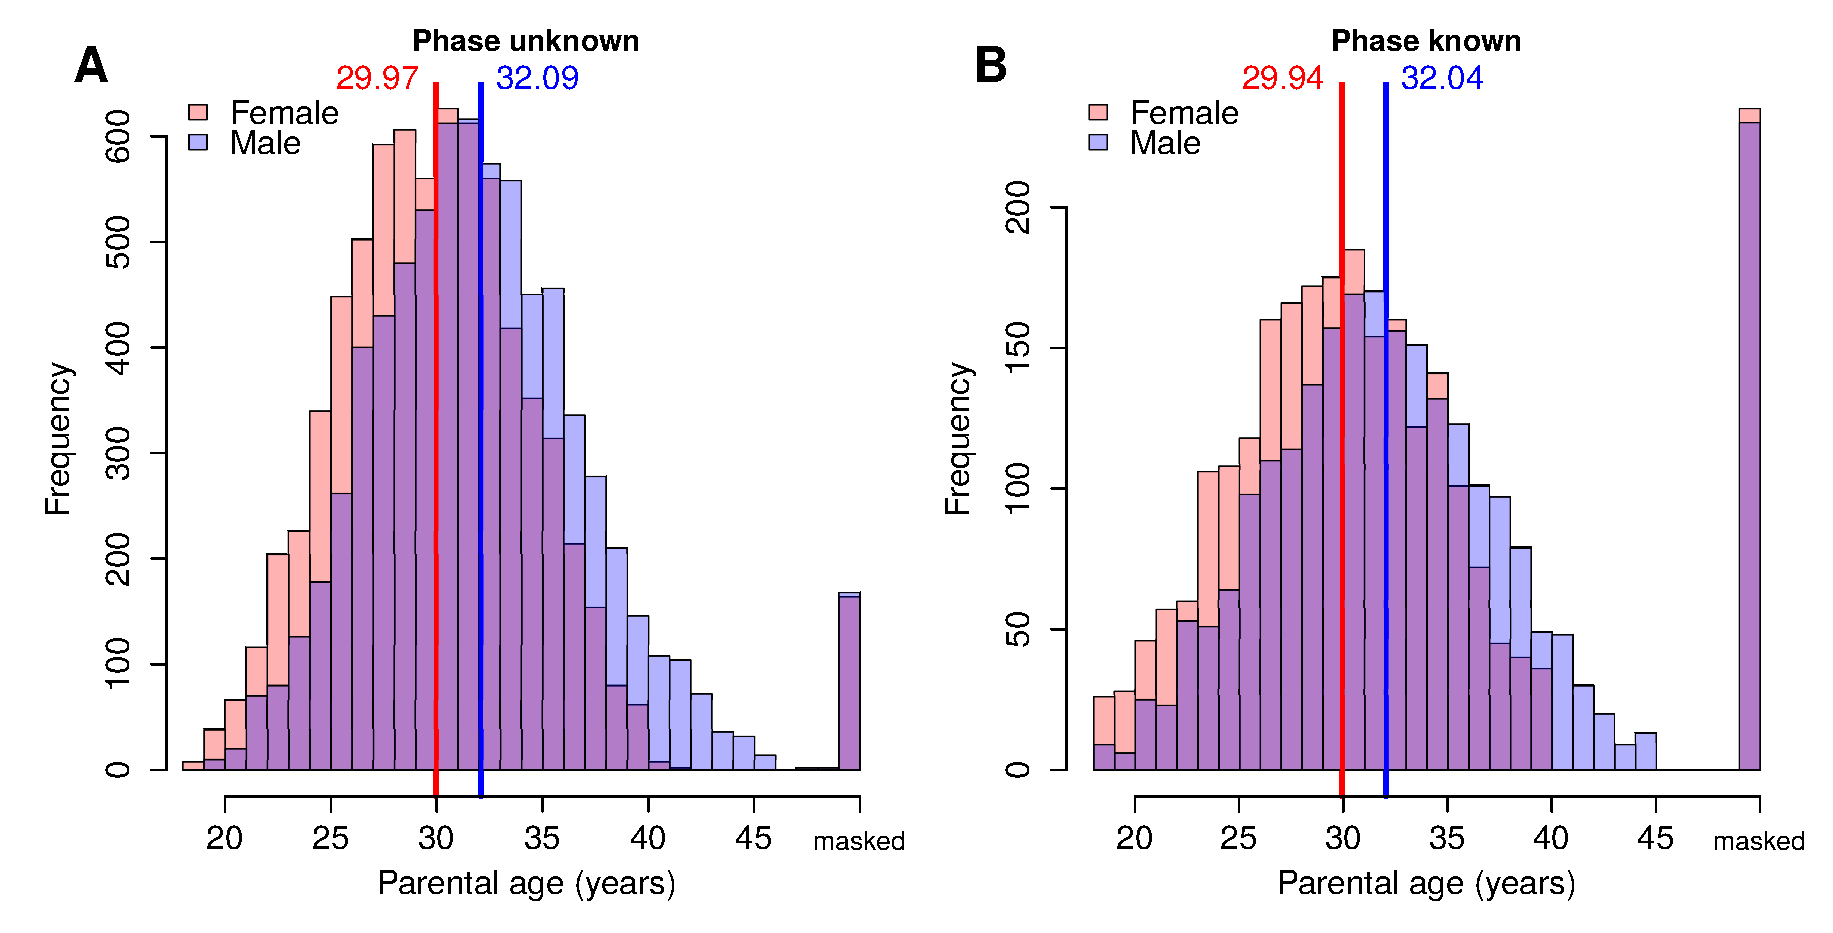
\includegraphics[width=\textwidth]{cointExtras/figs/ageHist_wMasked}
    \vspace{-20pt}
    \captionTitle{\textbf{Age distributions in the 23andMe dataset including older parents.}}{ 
        Phase-unknown parents are shown on the left panel (A), and phase-known parents, where ages were averaged across the children, are shown in the right panel (B).
        Additional data from older parents, in which the ages have been masked in females over 40 and males over 45 years old, are shown on the far-right of each distribution with the axis-label ``masked.''
        The vertical lines represent the mean of each distribution, excluding the older parents with masked ages.
    \label{fig:extrasAgeHist}}
\end{figure}
\clearpage}

\afterpage{
\begin{figure}[p]
    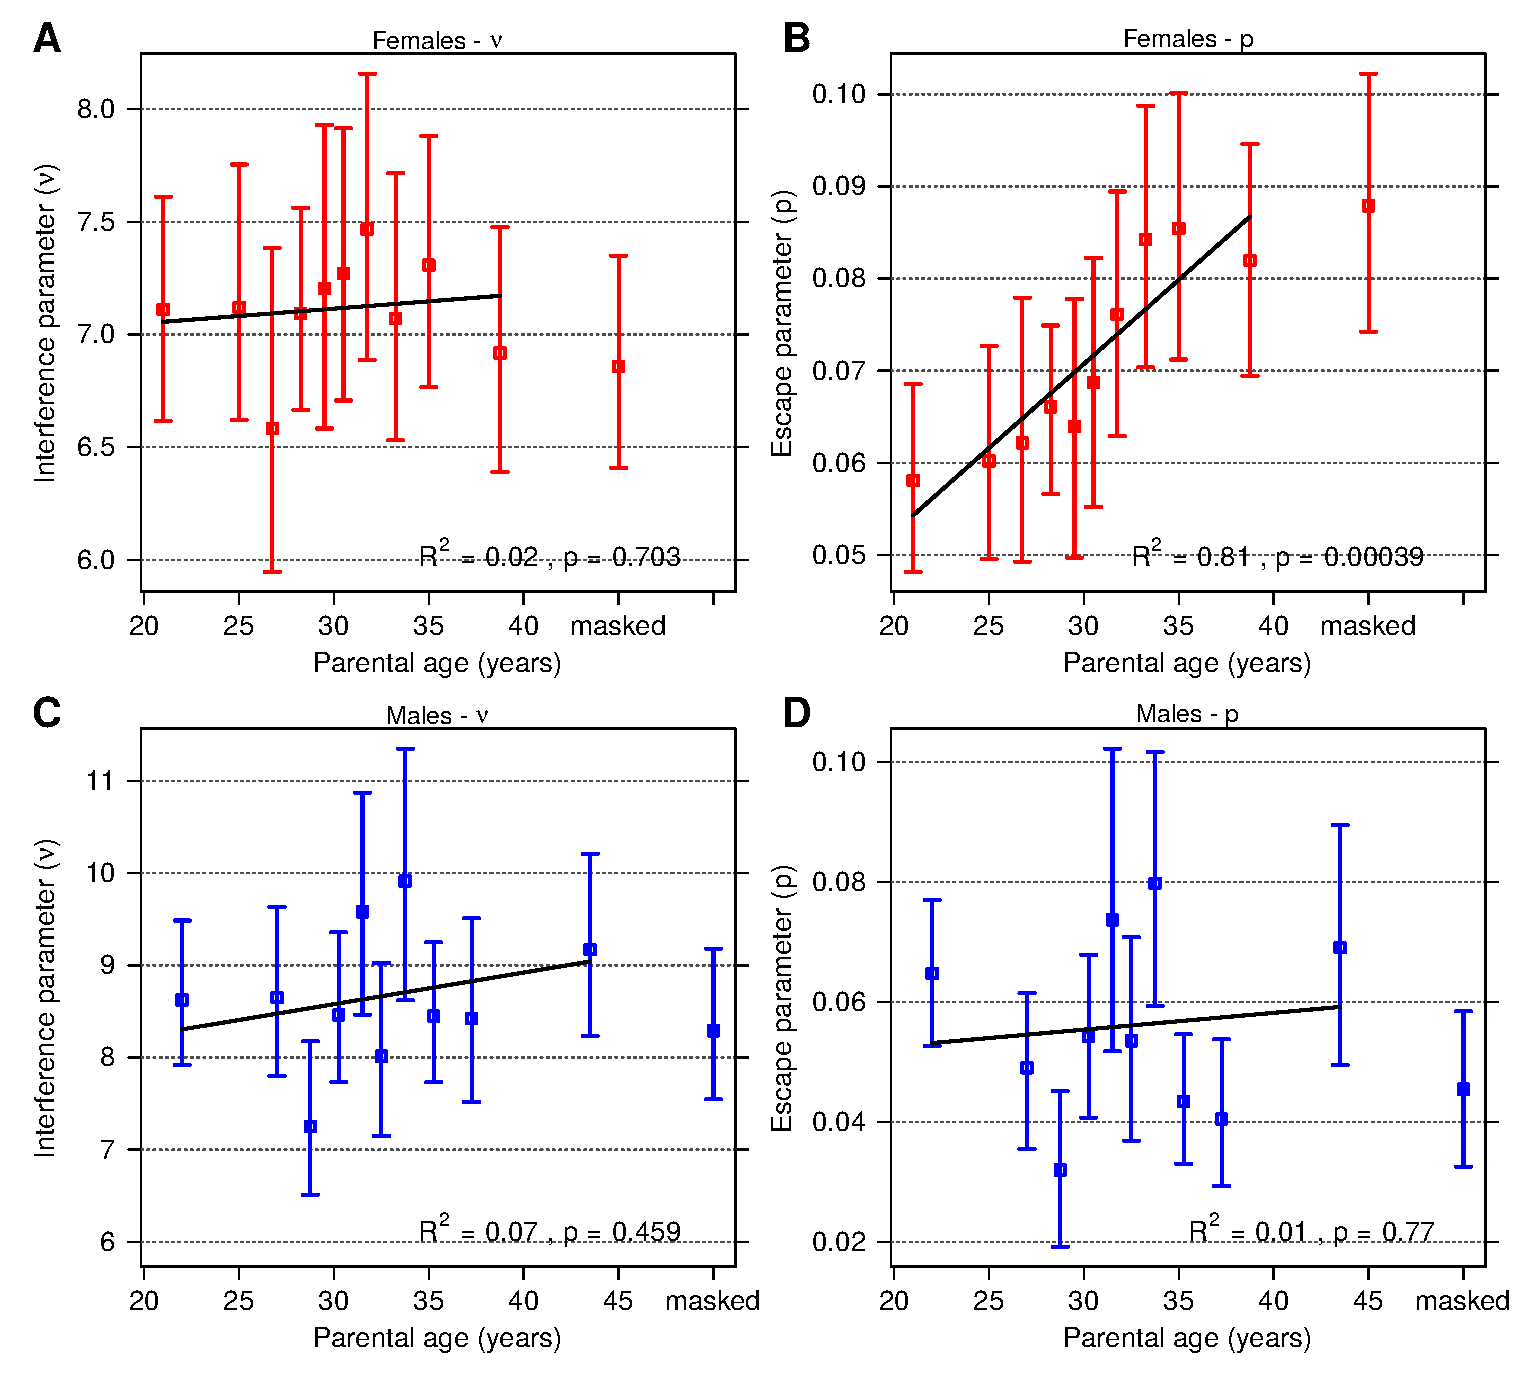
\includegraphics[width=\textwidth]{cointExtras/figs/coIntParam_wMasked}
    \vspace{-20pt}
    \captionTitle{\textbf{Crossover interference parameters as a function of age.}}{ 
        Parameter estimates for females are shown in the top two panels (A and B), males in the bottom two panels (C and D).
        Interference strength estimates ($\nu$) are shown in the left two panels (A and C), and estimates for the escape proportion are shown in the right panels (B and D).
        Data from older parents with masked ages are included in the plot with the axis label ``masked.''
        These older groups are excluded from the linear regression lines (shown in black).
    \label{fig:extrasCointAge}}
\end{figure}
\clearpage}



\afterpage{
\begin{figure}[p]
    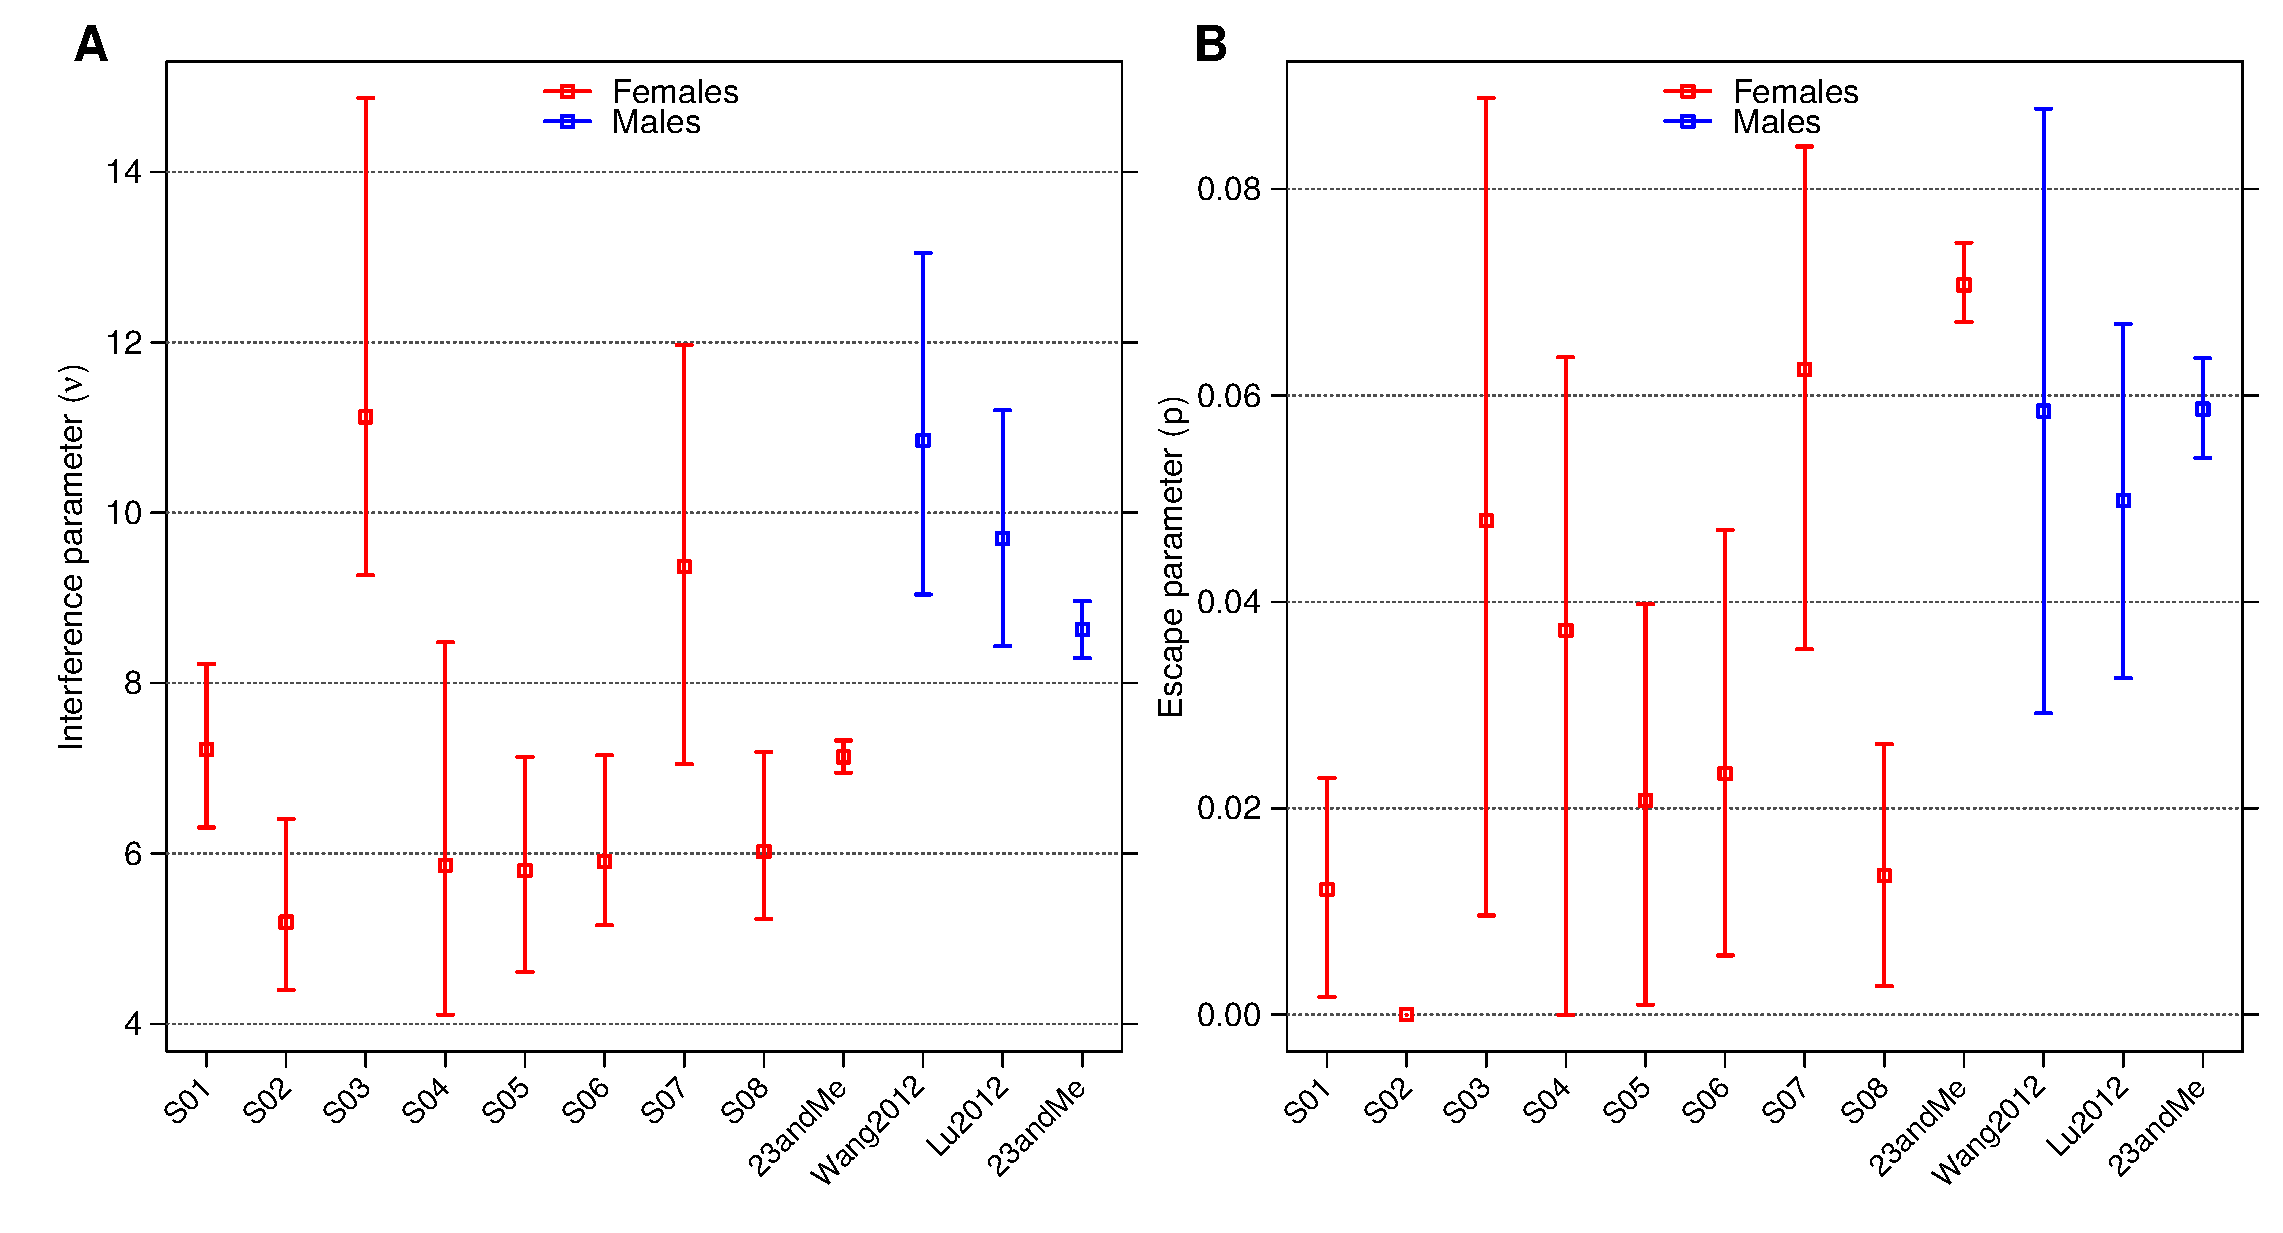
\includegraphics[width=\textwidth]{cointExtras/figs/coIntParam_public-individual}
    \vspace{-20pt}
    \captionTitle{\textbf{Crossover interference parameters in single cell data.}}{ 
        Interference parameter estimates are shown for the gamma escape model.
        The strength parameter is shown in panel A, and the escape parameter in panel B.
        Data points for females (red) represent data data generated by \citet{Hou2013}, representing 8 individuals.
        Data for males (in blue) comes from \citet{Lu2012} (n=99), \citet{Wang2012} (n=99).
        23andMe data\cite{Campbell2015} is provided for comparison and represents 2,184 females and 2,092 males).
    \label{fig:extrasCointSingle}}
\end{figure}
\clearpage}

% \subsection{Maternal age effect}

\clearpage
\section{Discussion}
The questions of how recombination properties vary on an individual basis and with age have long been outstanding.
I have presented here a series of analyses that attempt to shed light on these effects. %, some of which were addressed elsewhere in this thesis.

I have used an updated dataset which was previously presented without the age-masked individuals included here, both in this thesis (Chapter \ref{ch:cointEsc}), and in a peer-reviewed journal article\cite{Campbell2015}.
The original dataset was the first study of recombination in humans to find evidence for an increase in the proportion of events that escape crossover interference with increased age in females.
The original data was suggestive of an increasing de-regulation of events with age in females.
Considering the increased incidence of aneuploidy in older mothers\cite{Hassold2001}, it was suggested that these observations could be related.
Here, I have updated this finding to include data from older parents, which had been masked for privacy concerns.
The updated dataset validates and extends the original finding that interference escape increases in older mothers, but not fathers.
Although there is an overlap in the confidence intervals, the masked data in older mothers continues to increase from the previous bin and has no overlap with the youngest group, supporting the idea that the phenomenon is a linear increase.

In a separate analysis, I have taken previously published data from recombination studies that identified crossovers within individuals using multiple single cell assays.
These data provide a picture of how much variation can be expected within a single individual, which appears to vary substantially.
Although the number of individuals represented here is small, the techniques used to produce this data provide a promising avenue for future research as the cost and complexity to perform these analyses decreases.
In the future, such analyses could be performed on a much larger scale, and provide valuable insight into the variation of recombination properties within individuals.

\clearpage
\renewcommand{\bibname}{References}
\bibliographystyle{ccampbell_thesis}
\begingroup
    \setlength{\bibsep}{10pt}
    \linespread{1}\selectfont
    \bibliography{/home/ccampbell/Dropbox/papers/thesis-cointExtras}
\endgroup





%%%%%%%%%%%%%%%%%%%%%%%%%%%%%%
\begin{SingleSpace}
\chapter{A pedigree-based map of recombination in the domestic dog genome} \label{ch:dogPed}
%%%%%%%%%%%%%%%%%%%%%%%%%%%%%%

\noindent Christopher L Campbell$^1$ , Claude Bh\'{e}rer$^{1,2}$ , Bernice E Morrow$^1$ , Adam Boyko$^3$ , and Adam Auton$^{1*}$

\vspace{0.5cm}
\noindent This manuscript has been submitted to \textit{Genetics}. \\

\vspace{0.5cm}
\noindent $^1$ Department of Genetics, Albert Einstein College of Medicine, 1301 Morris Park Avenue, Bronx, New York 10461, USA. \\
\noindent $^2$ New York Genome Center, New York, New York 10013, USA \\
\noindent $^3$ Department of Biomedical Sciences, College of Veterinary Medicine, Cornell University, Ithaca, New York 14853, USA \\
\noindent $^*$ Former affiliation.

\vspace{0.5cm}
\begin{centering}
    Correspondence and requests for materials should be addressed to \\
    A.A.\ (email: \texttt{adam.auton@gmail.com}). \\
\end{centering}
\end{SingleSpace}

%%%%%%%%%%%%%%%%%%%%%%%%%%%%%%%%%%%%%%%
%%%%%%%%%%%%%%%%%%%%%%%%%%%%%%%%%%%%%%%

\begin{abstract}

Meiotic recombination in mammals has been shown to largely cluster into hotspots, which are targeted by the chromatin modifier PRDM9.
The canid family, including wolves and dogs, has undergone a series of disrupting mutations in this gene, rendering \textit{PRDM9} inactive.
Given the importance of \textit{PRDM9} it is of great interest to learn how its absence in the dog genome affects patterns of recombination placement.
We have used genotypes from domestic dog pedigrees to generate sex specific genetic maps of recombination in this species.
On a broad scale, we find that placement of recombination events in dogs is consistent with that in mice and apes, in that the majority of recombination occurs toward the telomeres in males, while female crossing over is more frequent and evenly spread along chromosomes.
It has been previously suggested that dog recombination is more uniform in distribution than that of humans,
however, we found that recombination in dogs is less uniform than humans. 
We examined the distribution of recombination within the genome, and 
find that recombination is elevated immediately upstream of the transcription start site, and around CpG islands, in agreement with previous studies, but find that this effect is stronger in male dogs.
We also find evidence for positive crossover interference influencing the spacing between recombination events in dogs, as has been observed in other species including humans and mice.
Overall our data suggests that dogs have similar broad scale properties of recombination to humans,
while fine-scale recombination is similar to other species lacking \textit{PRDM9}.

\end{abstract}


\section{Introduction}

The placement of recombination events within the genome is not random but instead is concentrated into regions known as hotspots. 
Recent work has identified the protein PRDM9 as responsible for targeting recombination events to hotspots\cite{Baudat2010,Myers2010,Parvanov2010}.
PRDM9 is active early in meiotic prophase\cite{Hayashi2005} and contains a zinc finger (ZF) array that binds to specific DNA motifs located at hotspot centers.
Upon DNA binding, PRDM9 trimethylates lysine 4 on histone H3, and is presumed to recruit cellular machinery to initiate recombination through an unknown mechanism.

Recombination hotspots are a common feature of eukaryote genomes but are not typically conserved between species.
For example, humans and chimpanzees have a complete absence of hotspot sharing, despite a high degree of overall DNA sequence identity\cite{Ptak2005,Winckler2005,Auton2012a}.
This change in hotspot location appears to be driven by the rapid evolution of the
ZF domain of \textit{PRDM9}, which is subject to strong selection in primates and rodents as well as a variety of ancient metazoans\cite{Oliver2009}.
Alterations to the ZF domain modify DNA motif recognition and binding specificity\cite{Oliver2009}
and hence contribute to a shifting landscape of active hotspots in the genome.

Evidence suggests that PRDM9 is required for the proper completion of meiosis.
Loss of \textit{PRDM9} causes sterility in male mice due to impairment of the progression of early meiotic prophase\cite{Hayashi2005}.
These mice, despite being sterile, still initiate double strand breaks (DSBs), and these breaks cluster into hotspots.
However, there is almost no overlap with hotspots that occur in mice with functional PRDM9, and these DSBs occur preferentially at promoters and CpG rich regions of the genome\cite{Brick2012}.  
This pattern is similar to that in other species lacking \textit{PRDM9}, including birds\cite{Singhal2015}, and yeast\cite{Lam2015}. 

The canid orthologue of \textit{PRDM9} has been inferred to have undergone multiple truncating mutations in the last exon, encoding the ZF array, and become a nonfunctional pseudogene\cite{Munoz-Fuentes2011}.
These mutations are shared within the Canidae family that includes dogs, coyotes, wolves, and foxes and must have accumulated after their divergence from pandas, who do not share the mutations, approximately 49 Mya\cite{Oliver2009,Munoz-Fuentes2011,Axelsson2012,Auton2013}.
Nonetheless, these species are all able to complete meiosis and reproduce,
which implies either that the function of PRDM9 in dogs is replaced by another gene or that recombination is able to complete successfully in its absence.
A rare homozygous loss of function mutation in \textit{PRDM9} has been recently reported in humans, in which a healthy mother was found to have mutations predicted to abolish both methlytransferase and DNA binding activity\cite{Narasimhan2016}, leading to 
 reduced crossover activity at PRDM9-dependent hotspots.
Transmission of the mutation was detected in one of her three healthy children, suggesting that humans may be able to successfully complete meiosis and remain fertile without functional PRDM9.

Despite the lack of \textit{PRDM9}, hotspot-like regions of recombination have been inferred in dogs from patterns of linkage disequilibrium (LD).
These hotspots differ qualitatively from those found in humans, appearing to have a lower intensity of recombination rate, and covering a wider genomic interval ($\sim$4-18 kb compared with $\sim$2 kb in humans)\cite{Axelsson2012,Auton2013}.
However, direct comparisons are complicated by differences in the general LD properties of the species arising from, for example, population demography\cite{Auton2013}.
Most striking is the observation that recombination is preferentially targeted towards CpG rich regions, such as those found in gene promoter regions,
which is similar to recombination patterns found in other species without \textit{PRDM9}.

Over the last three decades, the study of recombination in dogs has progressed from initial low-coverage linkage maps\cite{Mellersh1997,Neff1999}, bolstered by the assembly of a draft sequence of the dog genome\cite{Lindblad-Toh2005}, to higher-coverage pedigree maps\cite{Wong2010}, and high-resolution LD based maps from single nucleotide polymorphism (SNP) array and whole genome sequence data\cite{Axelsson2012,Auton2013}.
Here, we present a pedigree analysis of recombination in the domestic dog, \textit{Canis lupus familiaris}, using high-density SNP microarray data, which allows investigation of the sex-specific distribution of recombination in the dog genome.
Given the open questions regarding the role of PRDM9 in recombination, we compared the sex-specific landscape of recombination in the dog genome to that inferred from human pedigrees, and used this comparison to gain further insight into the effects of the presence or absence of PRDM9 on the mammalian recombination landscape.

%%%%%%%%%%%%%%%%%%%%%%%%%%%%%%
%%%%%%%%%%%%%%%%%%%%%%%%%%%%%%
\section{Methods}
%%%%%%%%%%%%%%%%%%%%%%%%%%%%%%
%%%%%%%%%%%%%%%%%%%%%%%%%%%%%%

\paragraph{Genotyping.}
The full dataset is derived from genomic analysis of 237 DNA samples, with 25 founder individuals (15 male, 10 female, pedigree structure shown in Figure \ref{fig:pedigree}) from a colony of Labrador Retriever and Greyhound crosses maintained at Cornell University for over 30 years\cite{Todhunter2003}.
Genotyping was performed using genomic DNA as described in \citet{Hayward2016} using Illumina CanineHD BeadChips that include more than 170,000 SNPs. 
All positions reported are given in canFam3.1 coordinates.

\paragraph{Filtering SNP data.}
To avoid spurious recombination calls due to genotyping error, we applied a set of filters on the variant data (outlined in Figure \ref{fig:pipeline}).
First, 586 SNPs were removed because they had missing genotypes in greater than 5\% of the samples.
We then used the PLINK\cite{Purcell2007} software (v1.07) to identify and remove a further 1,245 SNPs showing Mendelian errors in transmission (option \verb|--mendel|).
The error detection feature in the Merlin\cite{Abecasis2002} software (v1.1.2, option \verb|--error|) was used to identify and remove SNPs with genotypes that conflicted with pedigree structure and are likely to be genotyping errors.
Three iterations of Merlin error detection were performed, removing 1,363, 66, and 7 SNPs, respectively.
In total 2,771 unique SNPs were filtered out in the first round, leaving 163,400 SNPs for further analysis.

\paragraph{Calling crossover events.}
Autosomal recombination events were inferred using a combination of software tools.
First, the dog genomes were phased without using pedigree information using SHAPEIT2\cite{Delaneau2013} (v2.r790).
In order to avoid bias in our inference of recombination, we use a map file for phasing that has a constant rate of recombination (1 cM/Mb) between physical markers.
Following phasing, we used the duoHMM\cite{OConnell2014} software (v0.1.4) to call recombination events using a hidden Markov model approach.
The first duoHMM pass integrated pedigree structure information to correct phasing errors.
Then, duoHMM was used to call crossovers in each parent-child duo of the pedigree, of which only high-confidence events were retained (with probability $>$0.5).
The duoHMM method was also used to identify SNPs that have a high probability of genotyping error (which we removed if a SNP had a probability of error of $>$0.9).
This method has been demonstrated to have a high sensitivity and low false discovery rate when compared to a standard Lander-Green\cite{Lander1987} approach, such as that implemented in Merlin\cite{Abecasis2002}.

\paragraph{Filtering crossovers.}
Tightly clustered crossovers within individuals may occur naturally as a result of gene conversion, however another possibility is that genotype errors have caused false crossover calls.
In many cases in our data we found double crossovers that belonged to a shared parent, and are clustered within the genome.
Furthermore, these crossovers often used the same SNP for the interval boundaries.
This strongly suggests genotyping error as a likely cause.
We therefore removed any double crossovers if that cluster within 1 Mb, and if more than one meiosis transmitted from the same parent also has clustered crossovers with shared interval boundaries.

We further remove all crossovers attributed to meioses that have biologically abnormal crossover counts.
We define thresholds separately for males and females, with a distribution centered around the median crossover count, and defining the boundaries as 4 standard deviations from the sex specific median crossover count, with the standard deviation estimated via the robust estimator of 1.4826 MAD (median absolute deviation).

\paragraph{Construction of the genetic map.}
Due to the high level of inbreeding and homozygosity in domestic dogs,
it is often not possible to detect recombination events over a significant fraction of the genome within a given pedigree.
For example, if a breeding pair have few heterozygous variants towards the telomeric ends of a given chromosome, then events occurring within such regions will be largely invisible as they will not be flanked by informative markers.
Due to the high level of inbreeding within many dog samples, failure to account for this issue would result in an underestimate of the total map length.
To correct for this issue, we considered the location of informative markers within each pedigree, and scaled the genetic map accordingly.

In order for duoHMM to correctly identify a recombination event, it must be flanked by at least one heterozygous variant in the parent on each side.
For each parent-child duo for which we are able to make crossover calls, we identified the positions of the first and last heterozygous variant on each chromosome, which represent the genomic range in which we are able to observe a crossover.
Then, across all duos in our sample, we estimated the effective total number of meioses at each position along each chromosome (Figure \ref{fig:mstep}).
The effective number of meioses was used in place of a fixed number of meioses when calculating the recombination fraction at each genomic interval.

Recombination fractions were converted to genetic distances using Haldane's map function.
Comparing maps generated using the effective number of meioses to those using a fixed number of meioses, we observed an increase in autosomal map length for both females (59.7 cM) and males (49.2 cM), and an increase in the sex averaged map length of 48.6 cM (Figure \ref{fig:mstepIncrease}).

\paragraph{Estimation of crossover interference parameters.}
Crossover interference influences the spacing of crossover events when two or more occur on the same chromosome in the same meiosis.
We modeled the distance between these crossovers using two models.
The gamma model\cite{Broman2000} assumes that the inter-crossover distances follow a simple gamma distribution with shape $\nu$ and rate $2\nu$, where $\nu$ is a unitless measure of the strength of crossover interference,
with $\nu=1$ representing no crossover interference, $\nu<1$ representing negative interference (spaced closer than expected by chance), and $\nu>1$ indicating positive crossover interference (spaced further apart than expected).
The gamma-escape model, originally proposed by \citet{Housworth2003} provides an extension to the simple gamma model.
Here, crossovers that are governed by the interference effect ($\nu>1$) are modeled to coexist alongside a subset of crossovers that escape interference ($\nu=1$).
A second parameter, $p$, is included to allow the second class of ``escaping'' crossovers to exist in a mixture with the interfering crossovers, and represents the proportion of events that escape interference.
To measure crossover interference, we estimated the parameters $\nu$ and $p$ using a MATLAB software package (\url{https://github.com/auton1/interference}) previously developed to analyze interference in humans\cite{Campbell2015}.

In order to compare each of the fitted models, we used the Bayesian Information Criterion (BIC), which is given by:
$BIC = -2 \ln( L ) + k \ln( n )$
, where $L$ is the maximum likelihood estimation from the model fit, $k$ is the number of free parameters in the model, and $n$ is the number of observations.
The model with the smallest BIC is preferred.

\paragraph{Gene annotations.}
Gene annotations for canFam3.1 were downloaded from Ensembl (build 81).
We considered only protein coding genes located on the autosomes, and kept the longest isoform for each gene.

\paragraph{Thinning the human map.}
In order to make a valid comparisons between dogs and humans with respect to the proportion of recombination occupying a given amount of sequence, we took a number of steps to ensure the datasets are as similar as possible.
To enable sex-specific comparisons between the species, we used a human pedigree dataset (\citet{Campbell2015}) rather than an LD-based map.
As the human dataset is considerably larger, we randomly sampled 408 phase-known meioses (204 each from males and females) to match the size of the dog dataset.
We then reduced the SNP density of the human data.
The human dataset was genotyped on a microarray of higher density than we have available for dogs, which allows recombination events to be better resolved than what was possible for dogs.
We therefore thinned the human dataset in an attempt to match the recombination event resolution in dogs using an \textit{ad hoc} iterative process as follows: 
1) Determine the inter-SNP distances for the human and dog datasets,
2) find SNPs that cluster more tightly in humans
3) remove a random subset of SNPs within each of these clusters,
4) iterate until the inter-SNP distributions and overall medians are similar between the two species.
This iterative process yields a thinned framework of SNPs in the human dataset such that the new inter-SNP distances closely resemble those in dogs (Figure \ref{fig:interSNPdist}).
Following this thinning, we examined each individual crossover in the human data, and expanded the interval boundaries, if necessary, to the next available SNP in the newly selected framework.
New sex specific genetic maps were then generated from this thinned data and used for the comparison to dogs.

\paragraph{Data availability.}
Supplementary data for this study, including sex-specific genetic maps, filtered crossover calls, and genotype data are available at 
\\ \url{https://github.com/clcampbell/dog_recombination}.

%%%%%%%%%%%%%%%%%%%%%%%%%%%%%%%%%%%%%%%%%%%%%%%%%%
%%%%%%%%%%%%%%%%%%%%%%%%%%%%%%%%%%%%%%%%%%%%%%%%%%
\section{Results}
%%%%%%%%%%%%%%%%%%%%%%%%%%%%%%%%%%%%%%%%%%%%%%%%%%
%%%%%%%%%%%%%%%%%%%%%%%%%%%%%%%%%%%%%%%%%%%%%%%%%%

\paragraph{Building the genetic map.}
We used SNP array genotype data from 237 domestic dogs to map recombination in the canine genome. 
After applying a series of filtering steps on the SNP data (Figure \ref{fig:pipeline}),
we identified crossovers using duoHMM, a tool previously developed to identify recombination events in human data\cite{OConnell2014}.
Upon examination of the initial genetic maps, we identified several regions that exhibited biologically unrealistic recombination rates within concentrated physical regions and could be errors.
Several of these regions overlap known segmental duplications and copy number variants\cite{Nicholas2009,Chen2009}, which could account for the observed clustering of crossovers.
Another possible explanation is that the reference genome contains misplaced or inverted contigs within these regions, which would lead to calling of false crossover events on either side of the out of place region.
We removed all 435 variants within four such regions, totaling 5.6 Mb of sequence (Table \ref{tab:badregions}), and
a further 1,344 markers identified with the error detection feature of duoHMM. 

After re-calling crossovers on this filtered data, we found 8,312 autosomal recombination events.
We then identified and removed a set of clustered double crossovers, likely to be false calls, consisting of 90 events. 
Finally, we excluded meioses that have a biologically abnormal number of crossovers, excluding 3 female meioses (with 55, 41, and 119 crossovers), and 3 male meioses (with 5, 44, and 109 crossovers).
In total we excluded 463 out of 8,312 crossovers (5.6\%).

The filtered dataset consisted of 408 informative meioses, including 204 from females, and 204 from males.
There are 7,849 well supported crossover events that could be localized to a median size of 102.1 kb (Figure \ref{fig:intsize}).
The sex specific genetic maps had a mean resolution of less than 0.4 cM. 

\paragraph{Comparison to previous studies.}
To assess the accuracy and validity of our results, we compared our maps to those from previous studies.
We used sex specific maps from a previous pedigree analysis\cite{Wong2010} as well as a sex-averaged LD-based map generated from whole genome sequencing data of 51 village dogs\cite{Auton2013}.
At the broad scale there is close agreement to our sex averaged map from the LD map (Pearson $r=0.86$ at 5 Mb resolution), and from the pedigree sex averaged map ($r=0.75$, Figure \ref{fig:mapCor}A).
The male map has a higher agreement with previous studies (LD $r=0.80$, pedigree $r=0.76$, Figure \ref{fig:mapCor}B) than does the female map (LD $r=0.67$, pedigree $r=0.73$, Figure \ref{fig:mapCor}C).

\afterpage{
\begin{table}[p] \centering
    \begin{tabular}{|l|c|c|c|c|c|} 
        \hline Study & Year & Female (cM) & Male (cM) & Ratio & Sex avg.\ (cM) \\ \hline
        Mellersh et al.\cite{Mellersh1997} & 1997 & 1039 & 766 & 1.36 & 902.5 \\
        Neff et al.\cite{Neff1999} & 1999 & 1820 & 1290  & 1.41 & 1555 \\
        Wong et al.\cite{Wong2010} & 2010 & 2276 & 1909 & 1.19 & 2092.5 \\
        Axelsson et al.\cite{Axelsson2012} & 2012 &  &  &  & 3005 \\
        Auton et al.\cite{Auton2013} & 2013 &  &  &  & 2430 \\
        This study & 2016 & 2162 & 1816 & 1.19 & 1978 \\
    \hline \end{tabular}
    \caption{Autosomal map length estimates. Total map lengths are given in centimorgans, while the ratio represents the female to male map lengths. Sex specific map lengths are not available for the LD based maps.\label{tab:mapLengthsSummary}}
\end{table}
\clearpage}

Consistent with previous studies in dogs\cite{Wong2010,Mellersh1997,Neff1999}, and other mammals, including humans\cite{Coop2008,Campbell2015}, females have a longer map length (2162 cM) than males (1816 cM, Tables \ref{tab:mapLengthsSummary} and \ref{tab:mapLengths}).
We observed similar total genetic map lengths when compared to the \citet{Wong2010} pedigree study, although our maps are slightly shorter (by 114 cM in females, 93 cM in males, Table \ref{tab:mapLengthsSummary}).
Map length is strongly correlated to physical length in both sexes (male r$^2$=0.82, female r$^2$=0.83), and in the sex averaged maps (r$^2$=0.88; Figure \ref{fig:mapLength}).
The ratio of female to male autosomal map length is 1.19, equivalent to \citet{Wong2010}, but notably lower than that of humans at 1.56\cite{Campbell2015}.

\paragraph{Distribution of recombination.}
Previous studies showed that the recombination rate is elevated in telomeric regions and lower near the centromere, both in dogs\cite{Wong2010,Axelsson2012,Auton2013}, and other species\cite{DeMassy2013}.
We observed the same phenomenon, and this telomeric effect is largely driven by male recombination in both dogs and humans (Figures \ref{fig:distrRecomb}A, \ref{fig:recombRateHuman}).
The opposite pattern is seen in two chromosomes, 27 and 32, supporting previous evidence\cite{Wong2010} suggesting that the orientation of these chromosomes in the reference genome is likely reversed.
Based on this, we reverse the physical coordinates for these two chromosomes for all further analyses.

We quantified the amount of recombination occurring at the telomeric ends of each chromosome arm by estimating the proportion of total recombination occurring in a physical window located at the telomeric end (Figure \ref{fig:distrRecomb}B).
We found that 38.2\% of recombination occurred within 5 Mb of the telomere in males, compared with 9.7\% in females.
Human males have a roughly equivalent proportion within this same region (30.2\% within 5 Mb), while human females have a similar amount of recombination compared to female dogs (7.4\% within 5 Mb).
We conclude that, at a broad scale at least, the telomeric enrichment of recombination observed in male dogs is similar to that of humans.

\afterpage{
\begin{figure}[p]
    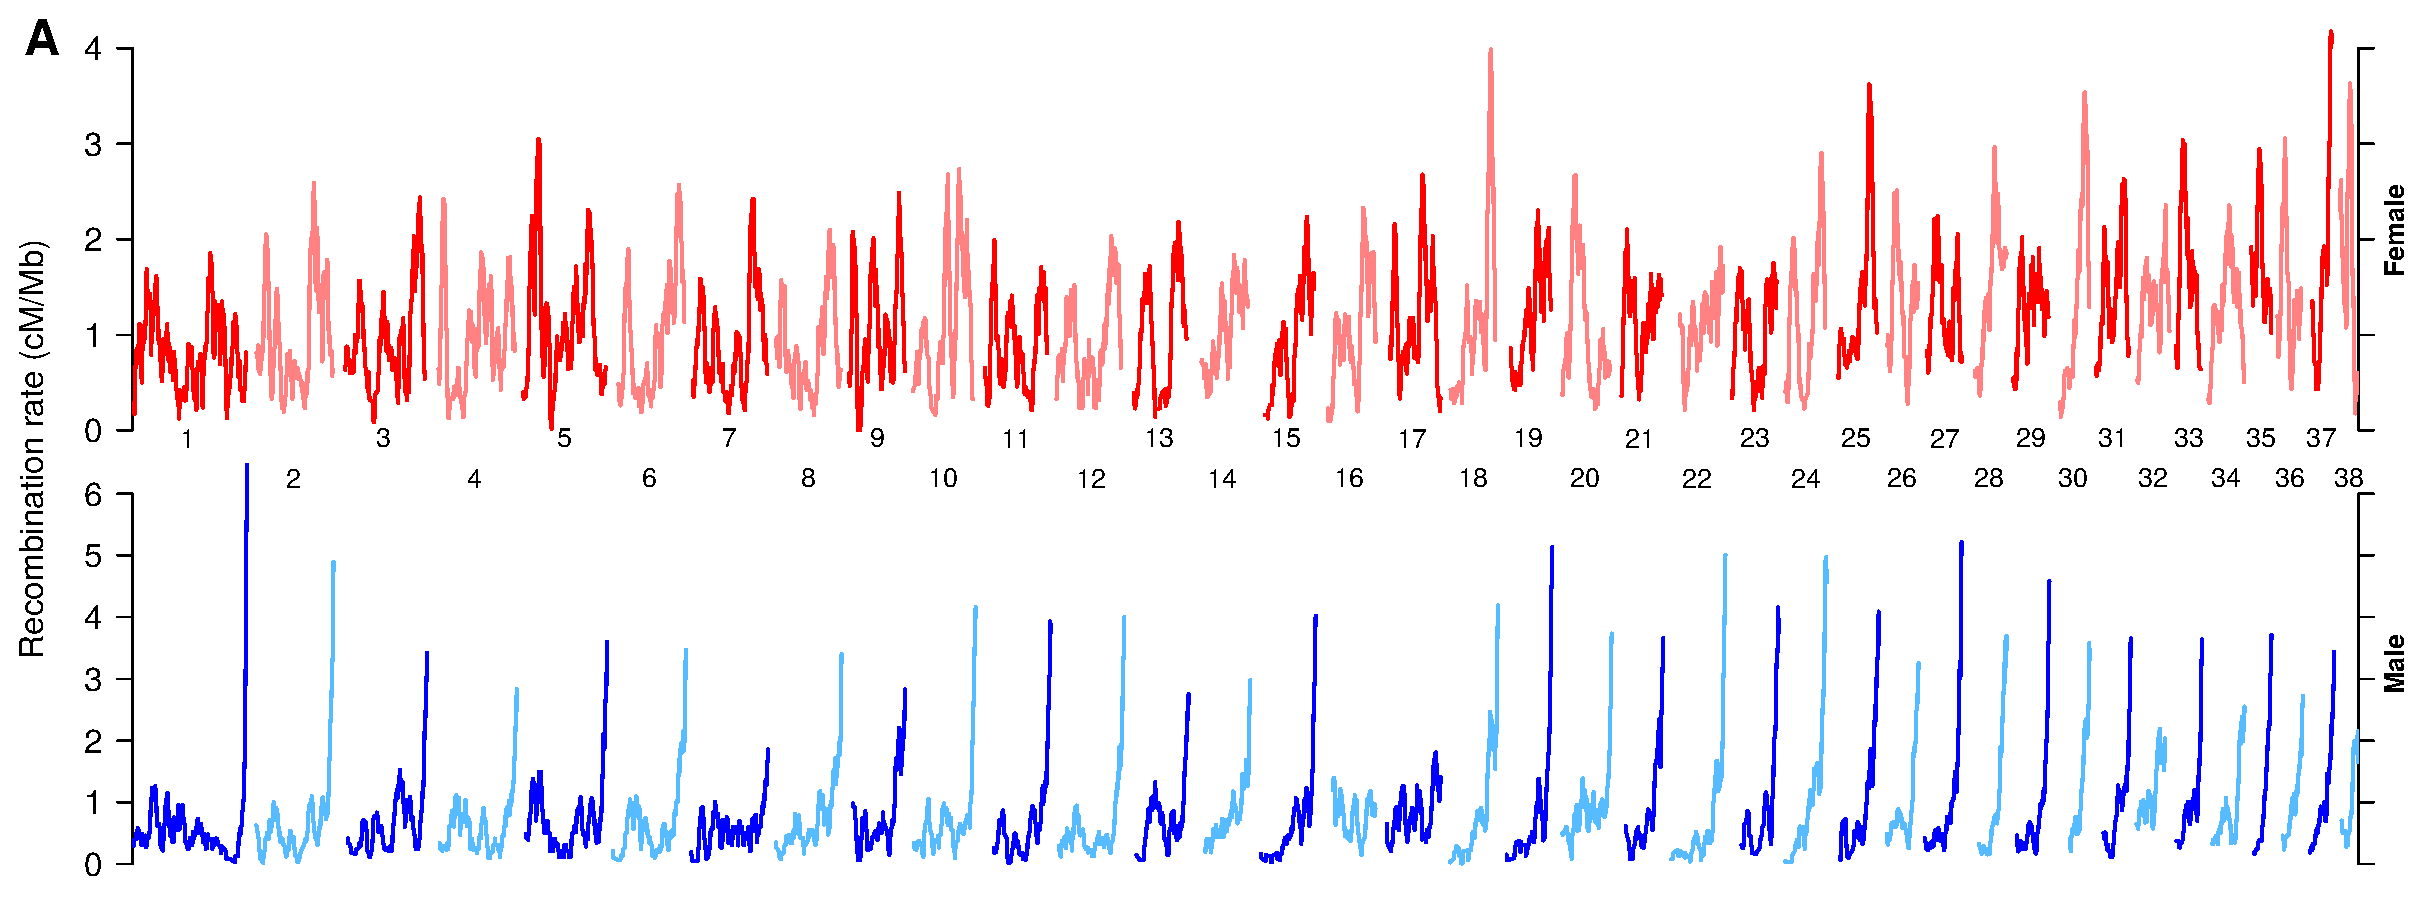
\includegraphics[width=\textwidth]{dogPed/figs/recomb_genome_dog}
    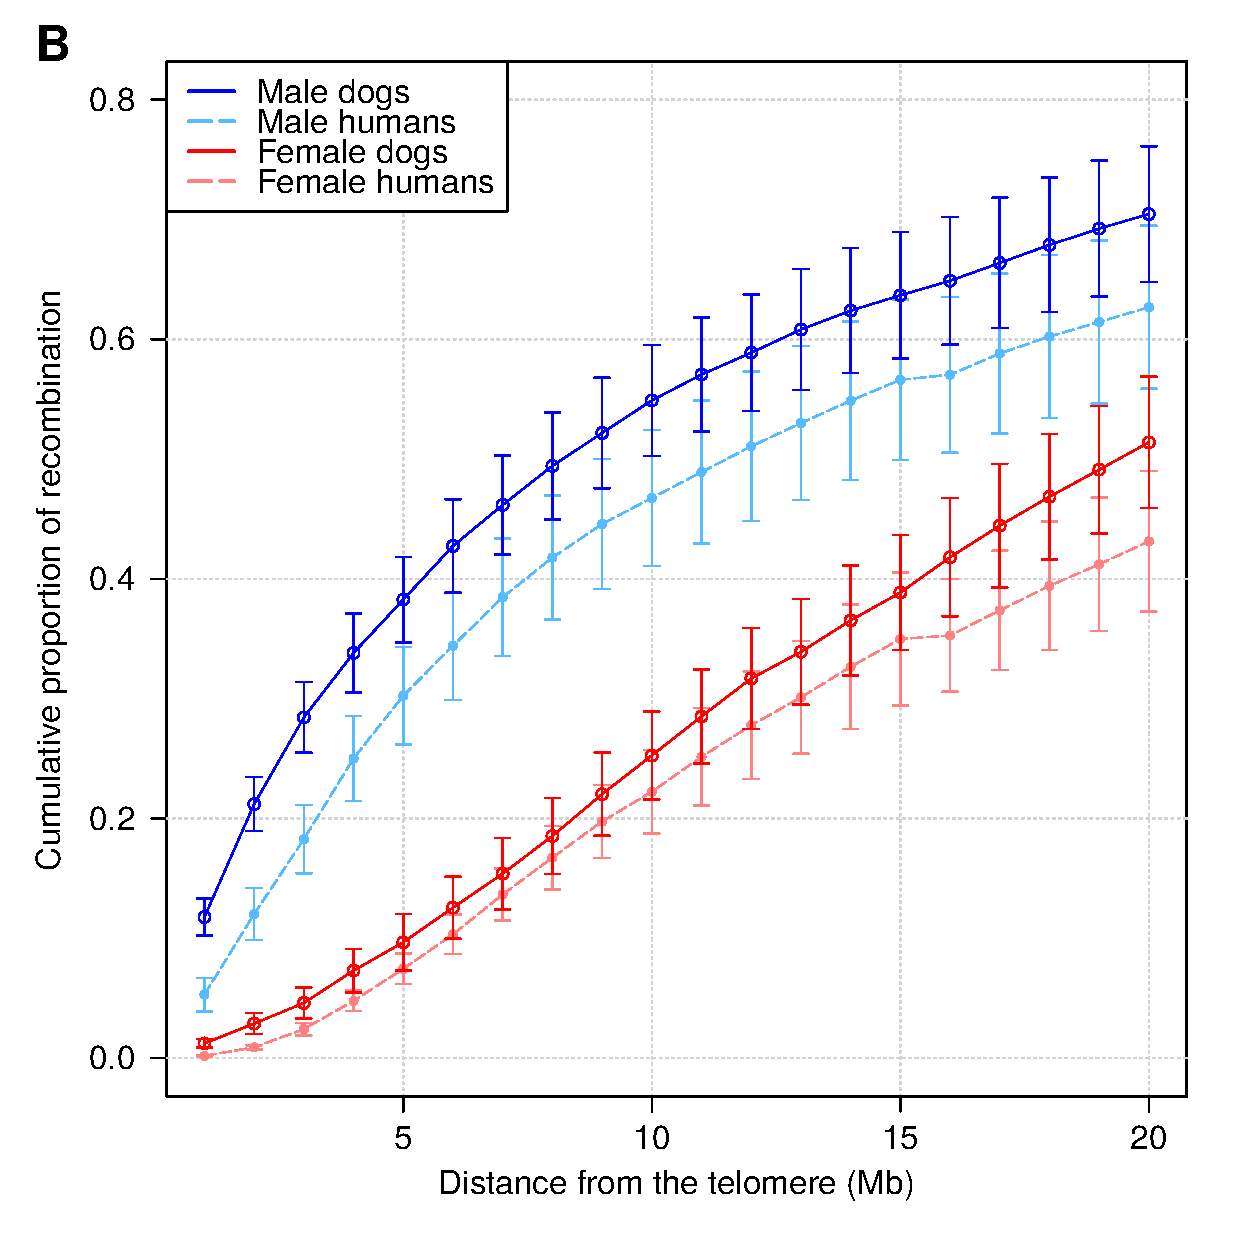
\includegraphics[width=0.5\textwidth]{dogPed/figs/propTelRecomb_Mb}
    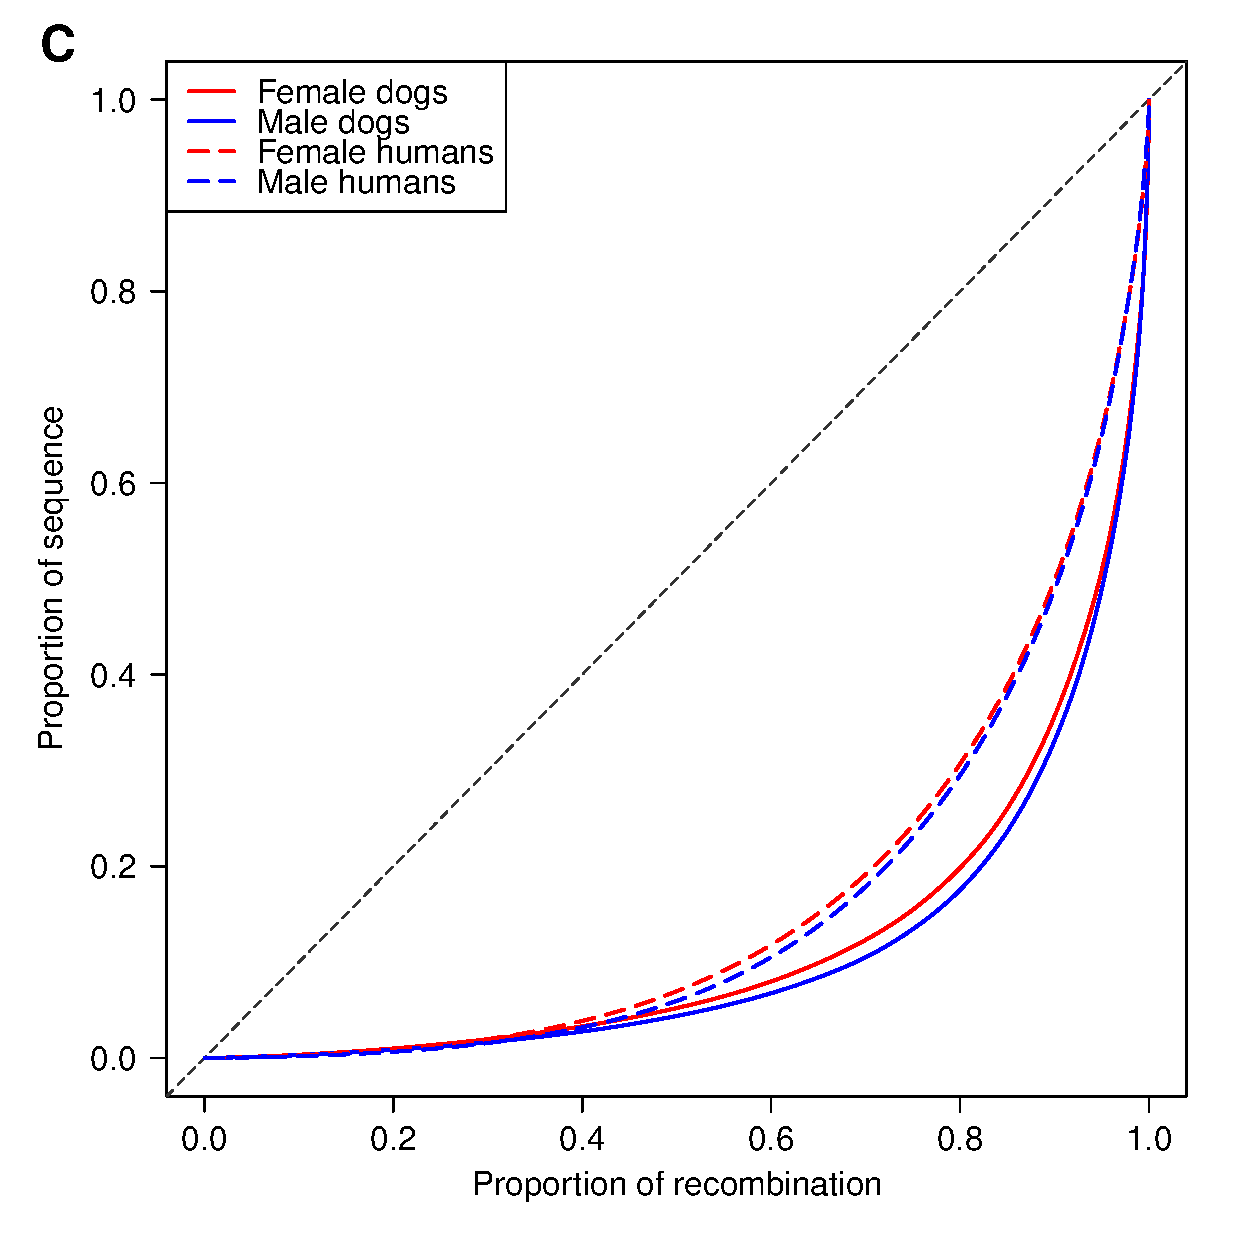
\includegraphics[width=0.5\textwidth]{dogPed/figs/8020plot_human-dog}
    \vspace{-15pt}
    \caption{The distribution of recombination across the genome.
        (A) Broad scale recombination rates differ between males and females.  Rates were smoothed at the 5 Mb scale. Chromosomes 27 and 32 are likely reversed in the canFam3.1 genome build, and are shown here with their physical coordinates reversed.
        (B) The proportion of recombination as a function of the distance from the telomeric end of each chromosome arm. Error bars represent a 95\% confidence interval.
        (C) Proportion of recombination occupying various fractions of the sequence. The human data were thinned to match the SNP density and meiosis count of the dog dataset.
        For all panels, males and females are shown in shades of blue and red, respectively. Human data in panels B and C is shown in dashed lines.
    \label{fig:distrRecomb}}
\end{figure}
\clearpage}


Previous observations using LD recombination maps have raised the possibility that dog recombination may be more uniform in distribution throughout the genome than in humans due to the loss of \textit{PRDM9}\cite{Axelsson2012,Auton2013}.
However, estimates from LD can be confounded by differences in the effective population size, which complicate such comparisons.
Pedigree-based studies should not be subject to the same confounding issues, and
to investigate this further, we examined the concentration of recombination rates across the genome using our pedigree maps, and compared this to human pedigree data\cite{Campbell2015}.
This analysis is sensitive to the marker coverage and crossover resolution, so the human genetic maps have been reduced in resolution to match that of the dog data (see Methods, Figures \ref{fig:8020supp}A and C).
We found that 80\% of recombination occurred in a smaller proportion of the dog genome (17.5\% male, 19.8\% female, Figure \ref{fig:distrRecomb}C) than previously reported in LD-based estimates.
In contrast to the LD-based findings, dog recombination is actually less uniform than in the human thinned data,
in which males have 29.5\%, and females 30.7\% of their sequence containing the majority (80\%) of recombination.
In addition, males of both species have more focused recombination when compared to females.
To address the possibility that differences in genome architecture or recombination rate distribution could account for these observations, we excluded telomeric regions from the analysis, and matched dog chromosomes with similarly sized human chromosome arms (Figures \ref{fig:8020supp}B and D), with similar results.
Therefore, it appears that crossovers are more concentrated within a smaller proportion of the dog genome than in humans, and that this effect is more pronounced in males of both species.

\paragraph{Recombination around genomic features.}

Starting from the observation that recombination is targeted to CpG islands concentrated at gene promoter regions\cite{Auton2013}, we looked for these effects in our data, and to what extent they are sex specific.
We found that recombination rates were elevated around the TSS, both in the sex averaged and male maps, but no peak was discernible in females (Table \ref{tab:recRates}, Figure \ref{fig:genomicFeatures}A).
Additionally, male recombination rate in the surrounding regions was higher than females, despite a lower genome wide recombination rate.
This observation that can be partially explained by a modest enrichment in the number of genes (31\%) occurring in the telomeric 25\% of each chromosome where male recombination is more frequent.
However, while the male background rate is higher in telomeric regions, males exhibited a peak at the TSS even in non-telomeric regions (Figure \ref{fig:TSScpgSplit}A and B).

Both male and female recombination estimates showed elevated recombination surrounding CpG islands (Table \ref{tab:recRates}, Figure \ref{fig:genomicFeatures}B).
The peak in male dogs was higher than females by 0.98 cM/Mb, with a high background rate in the surrounding sequence, which could be explained by
clustering of CpGs, as well as an enrichment of CpG islands in telomeric, male driven recombination regions (42\% in 25\% of sequence, Figure \ref{fig:TSScpgSplit}C and D).
After thinning CpG islands to a uniform density throughout the genome, the male and female background rates were more comparable, but the male peak remains higher, suggesting that recombination around CpG islands is dominated by males (Figure \ref{fig:cpgThinned}).
We also examined recombination rates around H3K4 trimethylation marks found via ChIPseq on dog spermatocytes\cite{Auton2013}.
As previously reported, the presence of these marks associated with elevated recombination rates, however this association can be explained by the proximity of CpG islands to H3K4me3 marks (Figure \ref{fig:H3K4panel}), and we saw no differences between males and females.

\paragraph{Crossover interference.}
Crossover interference, a phenomenon that affects the physical spacing between pairs of crossover events occurring during the same meiosis, acts in various species, including humans\cite{Campbell2015,Broman2000,Housworth2003}, mice\cite{Broman2002}, and cattle\cite{Sandor2012}.
To learn more about interference in dogs, we examined the distribution of inter-crossover distances in our dataset.
We fit two models of crossover interference, the gamma model\cite{Broman2000}, and the gamma-escape model\cite{Housworth2003} (also known as the Housworth-Stahl model).
The gamma-escape model is a mixture model that builds upon the gamma model, adding a subset of events that escape interference.

The no-interference model ($\nu=1$), had a poor fit, with a lack of double crossovers in close proximity, indicating that positive crossover interference must be acting to some degree in dogs.
When fitting the simple gamma model, estimates of interference strength in male and female dogs overlapped with each other. % ($\nu_{female}=5.22$, $\nu_{male}=3.73$).
These estimates are comparable to a cytological study in dogs measuring the distance between MLH1 foci, which mark crossovers ($\nu$=6.1)\cite{Basheva2008}.
Comparing to humans, female dogs have a stronger strength of interference than human females, while the estimates for males of both species overlap (Figure \ref{fig:cointGenome}A, Table \ref{tab:cointParams}).

\afterpage{
\begin{figure}[p]
    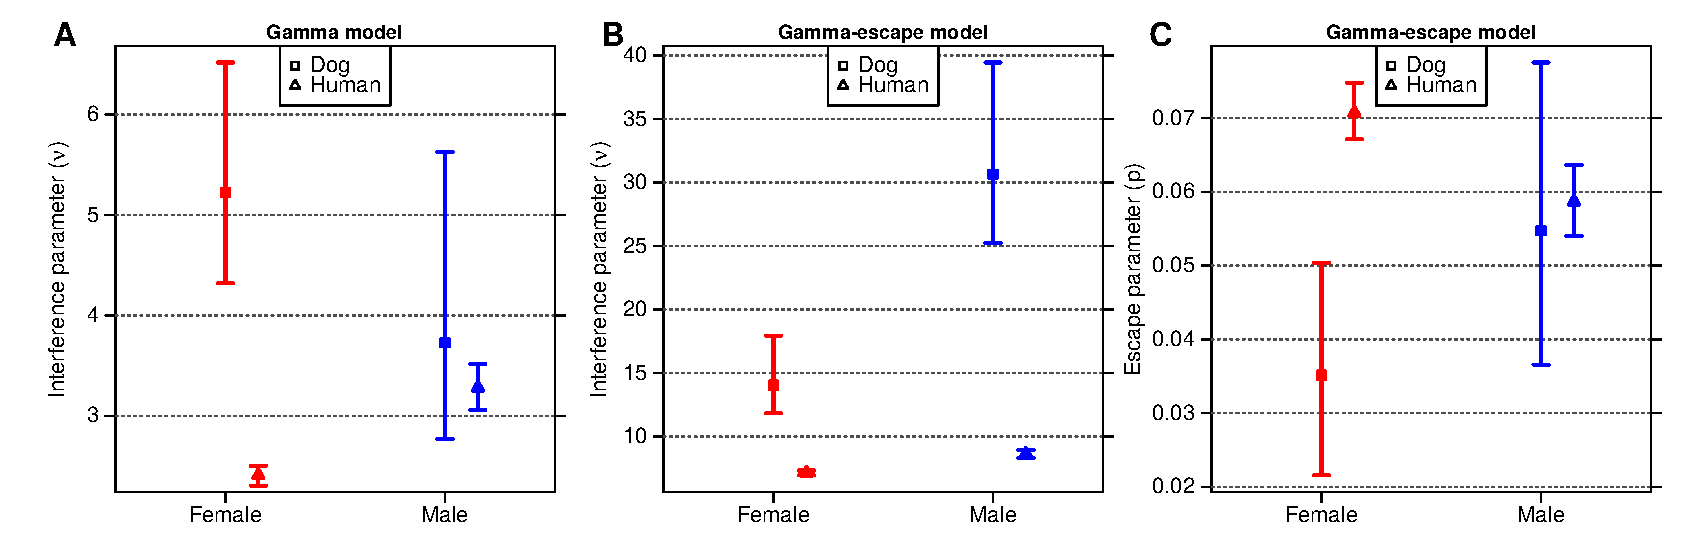
\includegraphics[width=\textwidth]{dogPed/figs/interferenceParameters_genome}
    \vspace{-20pt}
    \caption{Estimates of crossover interference parameters in the dog genome using the simple gamma model (A) and Housworth-Stahl gamma-escape model (B and C).
       Panels A and B show the interference strength parameter, $\nu$, for each model, while
       the right panel (C) shows the escape parameter, $p$, the proportion of events that escape interference.
       Males are shown in blue and females in red, while estimates for dogs are shown in boxes, and humans in triangles.
       The error bars represent a 95\% confidence interval estimated from 1000 bootstrap iterations. \label{fig:cointGenome}}
\end{figure}
\clearpage}

In the interference-escape model,
estimates of the strength of interference across the dog genome are higher in males than in females ($\nu_{female}=14.05$, $\nu_{male}=30.64$).
This trend is similar to that seen in humans, with stronger crossover interference in males, however the parameter estimates are higher by a factor of 2 in females, and more than 3 in males ($\nu_{female}=7.19$, $\nu_{male}=8.93$ in humans, Figure \ref{fig:cointGenome}B).
In contrast, male dogs have a similar proportion of escaping events to humans (5.5\% vs 5.9\%), while
female dogs have fewer events (3.5\%) escaping than human females (7.1\%, Figure \ref{fig:cointGenome}C).
We found support for both models of interference in the dog dataset, however
we used BIC to make a formal comparison of the goodness of fit for each model.
We found that in both sexes the gamma-escape model is preferred over the simple gamma model (Table \ref{tab:cointParams}), in agreement with previous findings supporting a two-pathway model of crossover interference in humans\cite{Housworth2003,Campbell2015}.


\afterpage{
\begin{table}[p] \centering
    \small
    \begin{tabular}{|c|c|c|c|c|c|} \hline 
            & \multicolumn{2}{c|}{Gamma model} & \multicolumn{3}{c|}{Gamma-escape model} \\ \hline
            & $\nu$ (95\% CI) & BIC & $\nu$ (95\% CI) & $p$ (95\% CI) & BIC \\ \hline
        Male dogs   & 3.73 (2.77-5.63) & 6617.1 & 14.05 (11.82-17.95) & 0.055 (0.037-0.078) & 6174.6 \\
        Female dogs & 5.22 (4.32-6.52) & 7580.9 & 30.64 (25.23-39.44) & 0.035 (0.022-0.050) & 7274.0 \\
        \hline
        Male humans   & 3.28 (3.06-3.51) & 99043.7  & 8.63 (8.29-8.96) & 0.059 (0.054-0.064) & 93205.3 \\
        Female humans & 2.41 (2.31-2.50) & 168775.7 & 7.13 (6.95-7.33) & 0.071 (0.067-0.075) & 156793.4 \\
    \hline \end{tabular}
    \caption{Autosomal crossover interference.  Parameter estimates are shown for both gamma and gamma-escape models for combined autosomes in dogs and humans.  Numbers in parentheses represent 95\% confidence intervals. BIC, Bayesian Information Criterion. \label{tab:cointParams}}
\end{table}
\clearpage}

To test if this difference reflects a change in interference parameters with parental age, as is observed in humans\cite{Campbell2015},
we divided our dataset by age into 7 approximately equal sized bins.
No differences were observed for crossover parameters for either model in any of the age groups (Figure \ref{fig:cointGenomeAge}).
However, we should note that bootstrapped estimates produce large error bars and there is likely insufficient power to adequately detect any age differences in this dataset.

When reducing the resolution of the human dataset (see Methods), we found that the parameter estimates were largely unchanged compared to those of the full resolution data, although with wider confidence intervals (Figure \ref{fig:cointGenomeThin}).
This provides confidence that parameter estimation using these models is robust to crossover interval size resolution and dataset power,
and that the parameters estimated from our dog data are likely to accurately reflect those of this dataset.

%%%%%%%%%%%%%%%%%%%%%%%%%%%%%%%%%%%%%%%%
%%%%%%%%%%%%%%%%%%%%%%%%%%%%%%%%%%%%%%%%
\section{Discussion}
%%%%%%%%%%%%%%%%%%%%%%%%%%%%%%%%%%%%%%%%
%%%%%%%%%%%%%%%%%%%%%%%%%%%%%%%%%%%%%%%%

Since the discovery of PRDM9 and its importance to recombination, questions about its full role have persisted.
While \textit{PRDM9} is under selection across a variety of species\cite{Oliver2009}, a notable subset are missing a functional version of this protein, raising questions regarding the landscape of recombination in these species.
Our pedigree study adds to existing work and provides insight into recombination in the absence of \textit{PRDM9}.
On a broad scale, our results are in agreement with those from previous studies, demonstrating that dog recombination is similar to other mammals, indicating that the presence or lack of \textit{PRDM9} does not change broad scale patterns of crossover placement.
In particular, a majority of crossing over occurs in telomeric regions in males, while female crossing over is both more frequent and more spread out.

We report a ratio of female to male map lengths of 1.19, equivalent to previous estimates from \citet{Wong2010}.
This groups domestic dogs with a large collection of species that exhibit sexual dimorphism in recombination in which the female has a higher rate of crossing over, including humans\cite{Campbell2015} and mice\cite{Cox2009}.
In contrast, cattle are one of the few species that have the opposite trend, with a recent study in domestic cattle estimating the male map length to be 10\% longer than females\cite{Ma2015}.
An interesting suggestion from this study was that the overall recombination rate in males may have been affected by artificial selection pressure.
Because artificial selection is more frequently focused on males, this can result in an increase in recombination if selection acts positively on recombination rate.
If true, it is not implausible that this selective pressure could have altered recombination in dogs during their domestication as well, something that could be revealed through a comparison to wolves, the closest ancestor to the modern domestic dog.
 
Initial estimates using LD maps in dogs indicated that 80\% of all recombination falls into a fairly large (30-46\%) amount of sequence\cite{Axelsson2012,Auton2013}, markedly more spread out than the $<$20\% figure seen in human LD maps\cite{hapmap2007}.
This supports the idea that PRDM9 acts to funnel recombination into hotspots in humans, and supports the hypothesis that dog recombination, lacking this hotspot specifying protein, is more uniform across the genome.
While further investigation is necessary,
our findings here, using pedigree data, suggest that dog recombination may actually be less uniform than humans.
Furthermore, in both species, males appear slightly more focused than females.  
This effect in humans could potentially be explained by a higher male hotspot usage\cite{Campbell2015}.
In dogs, this could be due to higher male rates around gene promoter regions and CpG islands that are concentrated towards the telomeres.
This concentration of recombination at functional genomic elements is not unique to dogs, but appears to be shared among a number of species lacking \textit{PRDM9}, including \textit{PRDM9} knockout mice\cite{Brick2012},
Arabidopsis, yeast\cite{Lam2015}, and birds\cite{Singhal2015}.

The concentration of recombination at these functional elements
supports a working model for \textit{PRDM9}-absent species, in which recombination occurs preferentially in regions of open chromatin.
Another implication is that recombination hotspots in dogs and other \textit{PRDM9}-absent species may be stable in evolutionary time, in contrast to current evidence against hotspot sharing in \textit{PRDM9} dependent species.
Since dog hotspots lack a strong motif that is likely to be targeted by a trans acting factor such as PRDM9\cite{Axelsson2012,Auton2013}, they are not likely to be subject to the hotspot paradox that acts to continually erode the binding capacity of hotspots, even as they are actively being used for recombination\cite{Myers2010}.
Evidence for hotspot stability has been found in two finch species, which share recombination hotspots that appear to be separated by tens of millions of years\cite{Singhal2015}, as well as four yeast species sharing hotspots over 15 million years of evolution\cite{Lam2015}.


The distribution of inter-crossover distances in dogs supports the existence of positive crossover interference in the dog genome.
Estimates of interference strength in the simple gamma model are roughly in line with those in humans.
However, our results favor the gamma-escape model, supporting the idea that two separate pathways contribute to recombination in dogs.
In this model, dog interference appears to be 2-3 times stronger than in humans, with a similar proportion of escaping events.
Interestingly, while an increase in interference escape with age has been observed in human females\cite{Campbell2015}, no such age effect was observed in dogs.
Accepting that our canine sample size would limit our ability to detect such effects, another
potential explanation is that, in contrast to humans, 
the timing of meiotic events in dogs is substantially different.
Recombination in human females begins and enters a potentially lengthy meiotic arrest prenatally, resuming just prior to ovulation.
In contrast, meiosis in female dogs begins later, in the neonatal period.
While recombination is complete prior to ovulation in humans, dogs ovulate immature oocytes, after which meiosis must complete before the oocyte becomes fertile, around 48 hours after ovulation\cite{Freixa1987,Chastant-Maillard2011}.

Overall, these results add to a growing body of research in non-human recombination genetics, 
and provide a step towards answering many open questions in canine recombination.
Further work is needed on larger and more diverse pedigrees, both in domestic dogs and other members of the Canidae family, including wolves, in order to form a more complete picture of recombination in this family.

\section{Acknowledgments}
We thank Yu Kong and Anthony Marcketta for their helpful discussions and assistance in the analysis of this data.
C.L.C.\ was supported by the Training Program in Cellular and Molecular Biology and Genetics, T32 GM007491.
C.B. was supported by a postdoctoral fellowship from the Fonds de la recherche en sant\'{e} du Qu\'{e}bec (FRQS).
Data in this paper are from a thesis to be submitted in partial fulfillment of the requirements for the Degree of Doctor of Philosophy in the Graduate Division of Medical Sciences, Albert Einstein College of Medicine, Yeshiva University.


%%%%%%%%%%%%%%%%%%%%%%%%%%%%%%%%%%%%%%%%
%%%%%%%%%%%%%%%%%%%%%%%%%%%%%%%%%%%%%%%%
\clearpage
\renewcommand{\bibname}{References}
\bibliographystyle{ccampbell_thesis}
\begingroup
    \setlength{\bibsep}{10pt}
    \linespread{1}\selectfont
    \bibliography{dogPed/dogPed}
\endgroup
%%%%%%%%%%%%%%%%%%%%%%%%%%%%%%%%%%%%%%%%
%%%%%%%%%%%%%%%%%%%%%%%%%%%%%%%%%%%%%%%%

\clearpage
%%%%%%%%%%%%%%%%%%%%%%%%%%%%%%
%%%%%%%%%%%%%%%%%%%%%%%%%%%%%%
% Supplement
%%%%%%%%%%%%%%%%%%%%%%%%%%%%%%
%%%%%%%%%%%%%%%%%%%%%%%%%%%%%%
\beginsupplement
\section{Supplementary Information}

\begin{table}[h] \centering
    \begin{tabular}{|c|c|c|c|c|} 
        \hline Chromosome & Start & End & Size & \# variants \\ \hline
        6 & 44745965 & 47085070 & 2339105 & 182 \\
        16 & 53878711 & 56703603 & 2824892 & 221 \\
        19 & 20011075 & 20320803 & 309728 & 24 \\
        32 & 38654394 & 38810281 & 155887 & 8 \\
        \hline &&   \textbf{Total}   &   \textbf{5629612}    &   \textbf{435} \\
    \hline \end{tabular}
    \captionTitle{\textbf{Regions removed from the dataset.}}{\label{tab:badregions}}
\end{table}

\begin{table}[p] \centering
    \scriptsize
    \begin{tabular}{|c|p{1.3cm}|p{1.3cm}|p{1.2cm}|p{0.8cm}|p{0.8cm}|p{0.8cm}|p{0.8cm}|p{0.8cm}|p{0.8cm}|p{0.8cm}|}
        \hline CFA & Physical (bp) & First position (bp) & Last position (bp) & Female (cM) & Mean female rate (cM/Mb) & Male (cM) & Mean male rate (cM/Mb) & Sex avg.\ (cM) & Sex avg.\ rate (cM/Mb) & No. markers \\ \hline
1 & 122,678,785 & 4,283,592 & 122,309,715 & 95.54 & 0.78 & 85.17 & 0.69 & 90.12 & 0.73 & 8284 \\
2 & 85,426,708 & 3,621,442 & 85,062,551 & 78.36 & 0.92 & 64.77 & 0.76 & 71.66 & 0.84 & 5550 \\
3 & 91,889,043 & 5,604,604 & 91,556,345 & 75.63 & 0.82 & 62.64 & 0.68 & 68.77 & 0.75 & 6681 \\
4 & 88,276,631 & 5,840,941 & 87,934,673 & 76.46 & 0.87 & 55.85 & 0.63 & 66.10 & 0.75 & 6231 \\
5 & 88,915,250 & 1,243,143 & 88,673,195 & 95.67 & 1.08 & 68.00 & 0.76 & 81.70 & 0.92 & 6432 \\
6 & 77,573,801 & 455,434 & 77,489,595 & 67.30 & 0.87 & 59.17 & 0.76 & 63.11 & 0.81 & 5320 \\
7 & 80,974,532 & 180,153 & 80,809,723 & 70.31 & 0.87 & 47.59 & 0.59 & 58.81 & 0.73 & 5778 \\
8 & 74,330,416 & 2,763,496 & 72,510,424 & 60.10 & 0.81 & 57.07 & 0.77 & 57.83 & 0.78 & 4846 \\
9 & 61,074,082 & 876,259 & 60,812,630 & 62.66 & 1.03 & 50.65 & 0.83 & 55.67 & 0.91 & 4293 \\
10 & 69,331,447 & 2,125,046 & 69,293,175 & 66.85 & 0.96 & 55.26 & 0.80 & 61.17 & 0.88 & 4573 \\
11 & 74,389,097 & 4,087,888 & 74,253,347 & 58.71 & 0.79 & 48.36 & 0.65 & 53.60 & 0.72 & 4557 \\
12 & 72,498,081 & 82,400 & 72,115,946 & 61.01 & 0.84 & 52.90 & 0.73 & 55.91 & 0.77 & 5364 \\
13 & 63,241,923 & 4,067,434 & 62,932,928 & 54.05 & 0.85 & 45.71 & 0.72 & 49.52 & 0.78 & 4749 \\
14 & 60,966,679 & 7,309,849 & 60,600,364 & 51.49 & 0.84 & 45.22 & 0.74 & 48.11 & 0.79 & 4153 \\
15 & 64,190,966 & 4,913,124 & 64,007,939 & 48.69 & 0.76 & 44.57 & 0.69 & 46.43 & 0.72 & 4372 \\
16 & 59,632,846 & 6,692,748 & 58,967,916 & 52.23 & 0.88 & 37.86 & 0.63 & 45.03 & 0.76 & 3829 \\
17 & 64,289,059 & 5,285,642 & 63,501,532 & 63.44 & 0.99 & 50.07 & 0.78 & 56.58 & 0.88 & 4731 \\
18 & 55,844,845 & 3,203,856 & 55,355,125 & 55.33 & 0.99 & 52.01 & 0.93 & 53.71 & 0.96 & 4014 \\
19 & 53,741,614 & 3,189,264 & 53,349,320 & 53.22 & 0.99 & 49.99 & 0.93 & 52.29 & 0.97 & 3733 \\
20 & 58,134,056 & 4,356,904 & 58,000,062 & 52.64 & 0.91 & 55.38 & 0.95 & 53.59 & 0.92 & 4140 \\
21 & 50,858,623 & 4,450,666 & 50,719,350 & 51.66 & 1.02 & 44.16 & 0.87 & 47.84 & 0.94 & 3706 \\
22 & 61,439,934 & 2,513,263 & 61,217,407 & 52.21 & 0.85 & 49.67 & 0.81 & 50.57 & 0.82 & 4422 \\
23 & 52,294,480 & 1,203,392 & 52,291,577 & 49.31 & 0.94 & 44.47 & 0.85 & 46.63 & 0.89 & 3928 \\
24 & 47,698,779 & 1,029,209 & 47,233,919 & 49.71 & 1.04 & 53.74 & 1.13 & 51.50 & 1.08 & 3625 \\
25 & 51,628,933 & 6,038,820 & 51,469,123 & 56.49 & 1.09 & 48.57 & 0.94 & 52.44 & 1.02 & 3922 \\
26 & 38,964,690 & 2,407,850 & 38,657,286 & 46.66 & 1.20 & 41.16 & 1.06 & 43.81 & 1.12 & 2853 \\
27 & 45,876,710 & 444,525 & 42,191,669 & 48.31 & 1.05 & 48.70 & 1.06 & 47.01 & 1.02 & 3354 \\
28 & 41,182,112 & 4,526,049 & 40,963,512 & 51.11 & 1.24 & 39.62 & 0.96 & 45.41 & 1.10 & 3074 \\
29 & 41,845,238 & 913,671 & 41,543,120 & 49.96 & 1.19 & 42.06 & 1.01 & 44.75 & 1.07 & 3017 \\
30 & 40,214,260 & 5,433,983 & 39,826,282 & 43.89 & 1.09 & 37.30 & 0.93 & 40.20 & 1.00 & 2942 \\
31 & 39,895,921 & 580,882 & 39,466,279 & 51.82 & 1.30 & 38.07 & 0.95 & 44.32 & 1.11 & 2855 \\
32 & 38,810,281 & 114,049 & 37,999,255 & 46.13 & 1.19 & 41.68 & 1.07 & 43.78 & 1.13 & 2746 \\
33 & 31,377,067 & 447,033 & 30,994,965 & 45.46 & 1.45 & 36.01 & 1.15 & 40.75 & 1.30 & 2320 \\
34 & 42,124,431 & 624,977 & 41,979,553 & 48.69 & 1.16 & 38.71 & 0.92 & 43.36 & 1.03 & 3239 \\
35 & 26,524,999 & 1,164,664 & 26,257,078 & 41.87 & 1.58 & 30.59 & 1.15 & 35.88 & 1.35 & 2171 \\
36 & 30,810,995 & 251,708 & 30,523,428 & 41.77 & 1.36 & 29.61 & 0.96 & 35.95 & 1.17 & 2286 \\
37 & 30,902,991 & 1,364,851 & 30,583,437 & 45.59 & 1.48 & 36.18 & 1.17 & 40.42 & 1.31 & 2333 \\
38 & 23,914,537 & 246,006 & 23,695,770 & 41.67 & 1.74 & 27.38 & 1.15 & 33.68 & 1.41 & 1895 \\
 \hline &  &  & \textbf{Total} & 2161.99 & 0.98 & 1815.91 & 0.82 & 1978.01 & 0.90 & 156,318 \\
\hline \end{tabular}
\captionTitle{\textbf{Physical and genetic chromosome lengths.}}{ \label{tab:mapLengths}}
\end{table}

\begin{table}[p] \centering
    \begin{tabular}{|c|c|c|c|c|} \hline 
        & Size (kb) & Male rate & Female rate & Difference (male - female) \\ \hline
        TSS upstream & 400 & 1.01 & 0.92 & 0.09 \\
        TSS & 50 & 1.12 & 0.92 & 0.20 \\
        TSS downstream & 400 & 1.03 & 0.94 & 0.09 \\
        \hline
        CpG upstream & 400 & 1.84 & 0.95 & 0.89 \\
        CpG island & 50 & 2.09 & 1.11 & 0.98 \\
        CpG downstream & 400 & 1.75 & 0.97 & 0.78 \\
    \hline \end{tabular}
    \captionTitle{\textbf{Recombination rate around TSS and CpG islands.}}{ Recombination rates are given in cM/Mb and were estimated in 10kb bins, and averaged over the indicated window.
        Rates surrounding CpG islands represent a 50kb window centered around the CpG island, while rates for the TSS are given as a 50kb bin ending at the TSS, capturing the elevated rate immediately upstream.
    \label{tab:recRates}}
\end{table}

\clearpage

\begin{figure}[p]
    \centering
    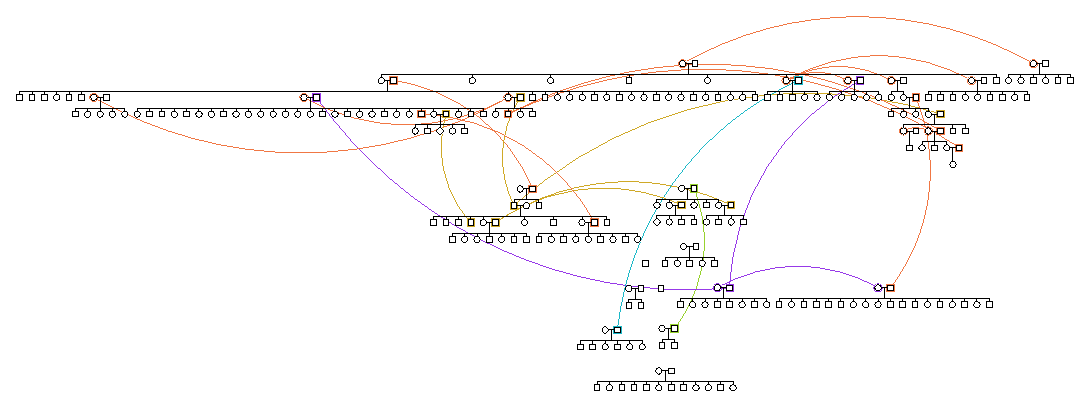
\includegraphics[width=\textwidth]{dogPed/suppfigs/dogPedigreePlot}
    \vspace{-5pt}
    \captionTitle{\textbf{Structure of the dog pedigree.}}{
        Males are represented by squares, females by circles.
        Colored lines indicate individuals repeated on the plot, that are involved in more than one mating pair.
    \label{fig:pedigree}}
\end{figure}

\begin{figure}[p]
    \centering
    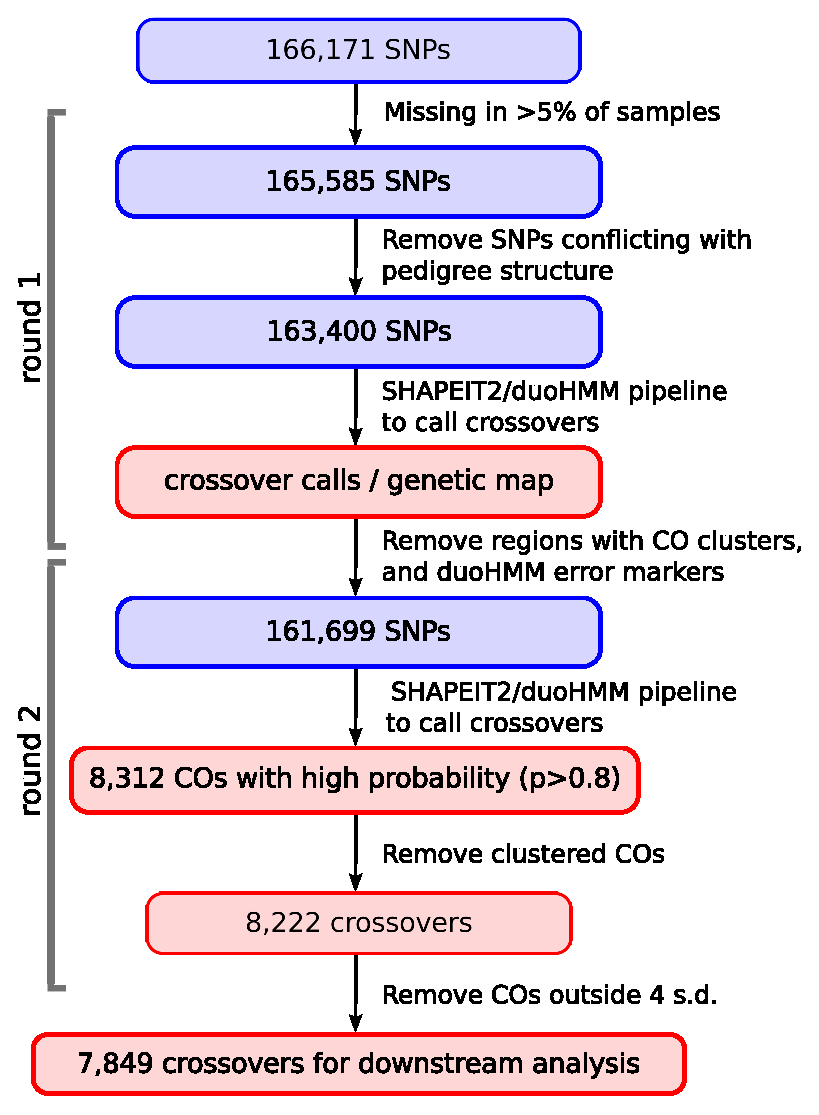
\includegraphics[height=0.6\textheight]{dogPed/suppfigs/pipeline}
    \vspace{-5pt}
    \captionTitle{\textbf{Overview of the analysis pipeline.}}{
        CO, crossovers; s.d., standard deviation.
    \label{fig:pipeline}}
\end{figure}

\begin{figure}[p]
    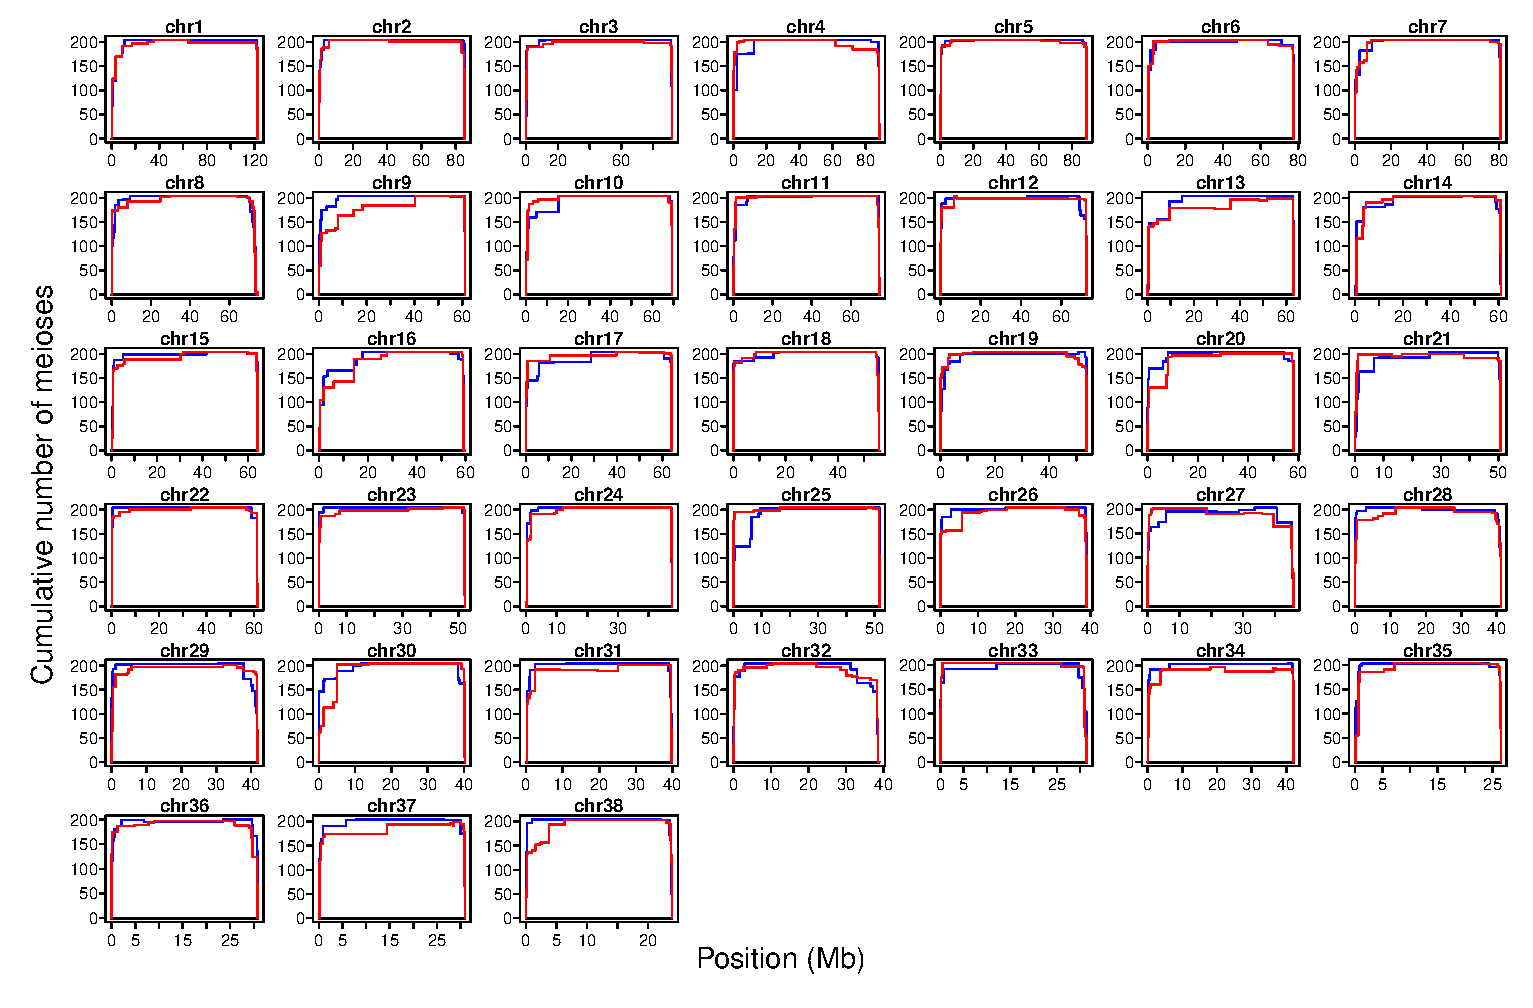
\includegraphics[width=\textwidth]{dogPed/suppfigs/informativeMeioses_step_duohmm2}
    \vspace{-20pt}
    \captionTitle{\textbf{The effective number of meioses as a function of physical position is shown along each chromosome.}}{
    Red curves represent females (n=204), blue curves represent males (n=204). \label{fig:mstep}}
\end{figure}

\begin{figure}[p]
    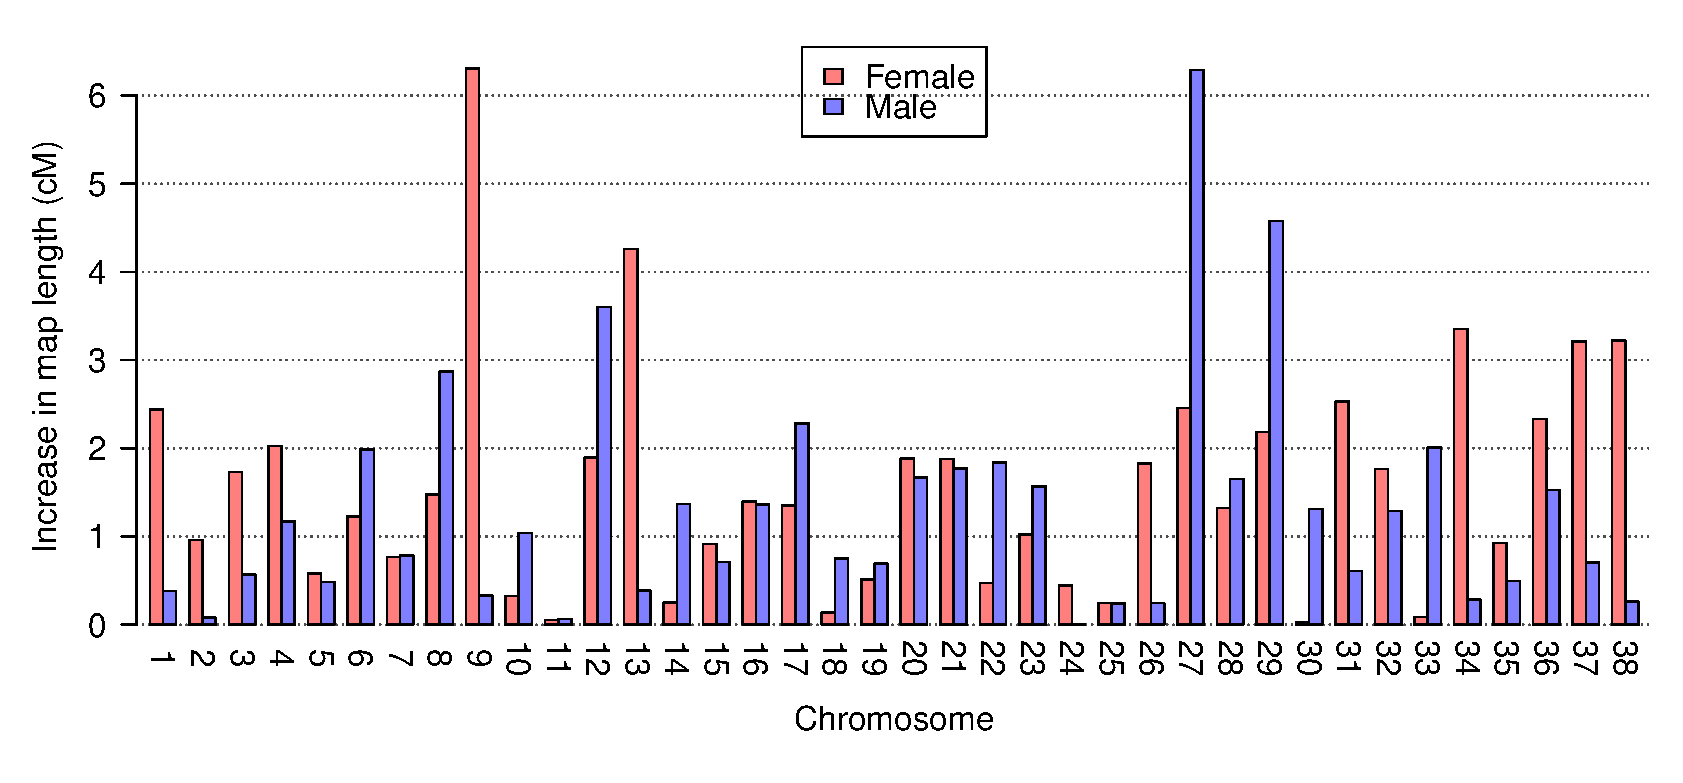
\includegraphics[width=\textwidth]{dogPed/suppfigs/mapLength_increase}
    \vspace{-20pt}
    \captionTitle{\textbf{Increase in map length in each chromosome after accounting for the effective number of meioses.}}{
    Each bar represents the difference in map length after taking into account a reduced number of observable meioses towards chromosome ends compared to the map length calculated using a fixed number of meioses (n=204 for females in red, n=204 for males, blue). \label{fig:mstepIncrease}}
\end{figure}

\begin{figure}[p]
    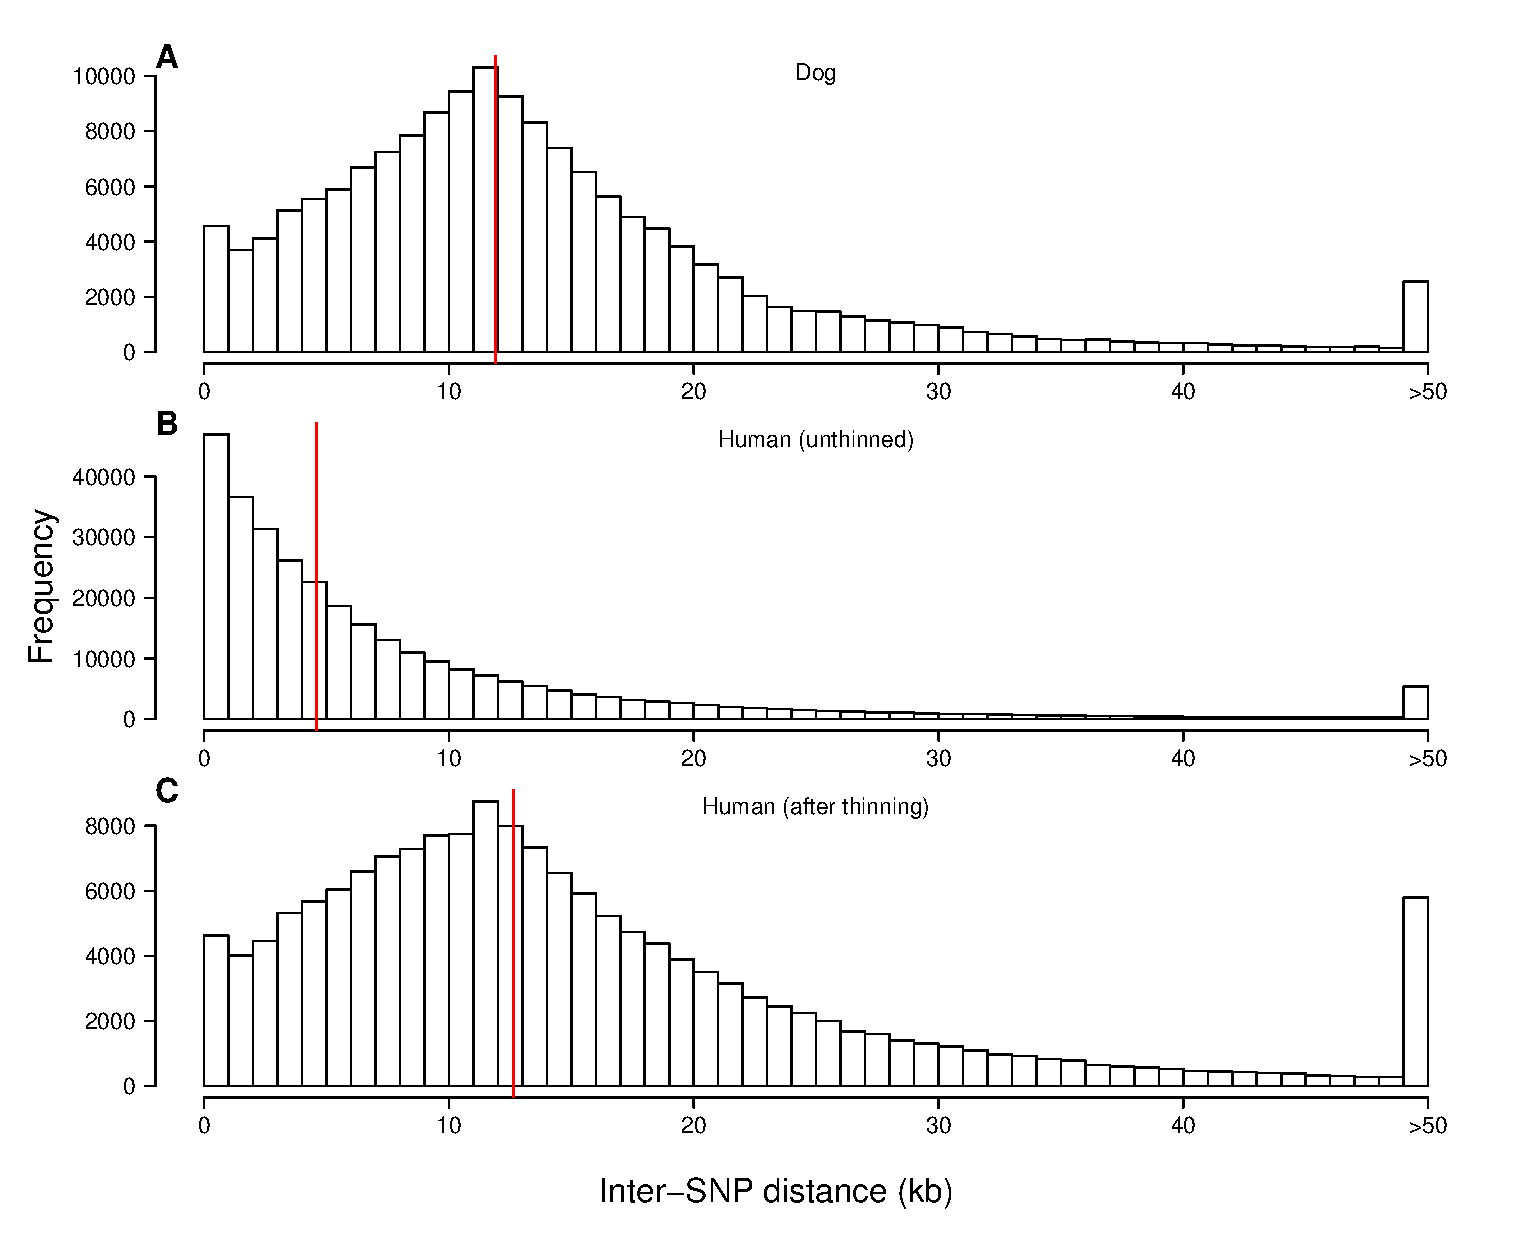
\includegraphics[width=\textwidth]{dogPed/suppfigs/interSNPdist_thinning}
    \vspace{-15pt}
    \captionTitle{\textbf{Distribution of inter-SNP distances in the dog data}}{
    (A), the human data prior to thinning (B), and the human data after the thinning procedure (C). The red line represents the median inter-SNP distance for each distribution.  \label{fig:interSNPdist}}
\end{figure}

\begin{figure}[p]
    \centering
    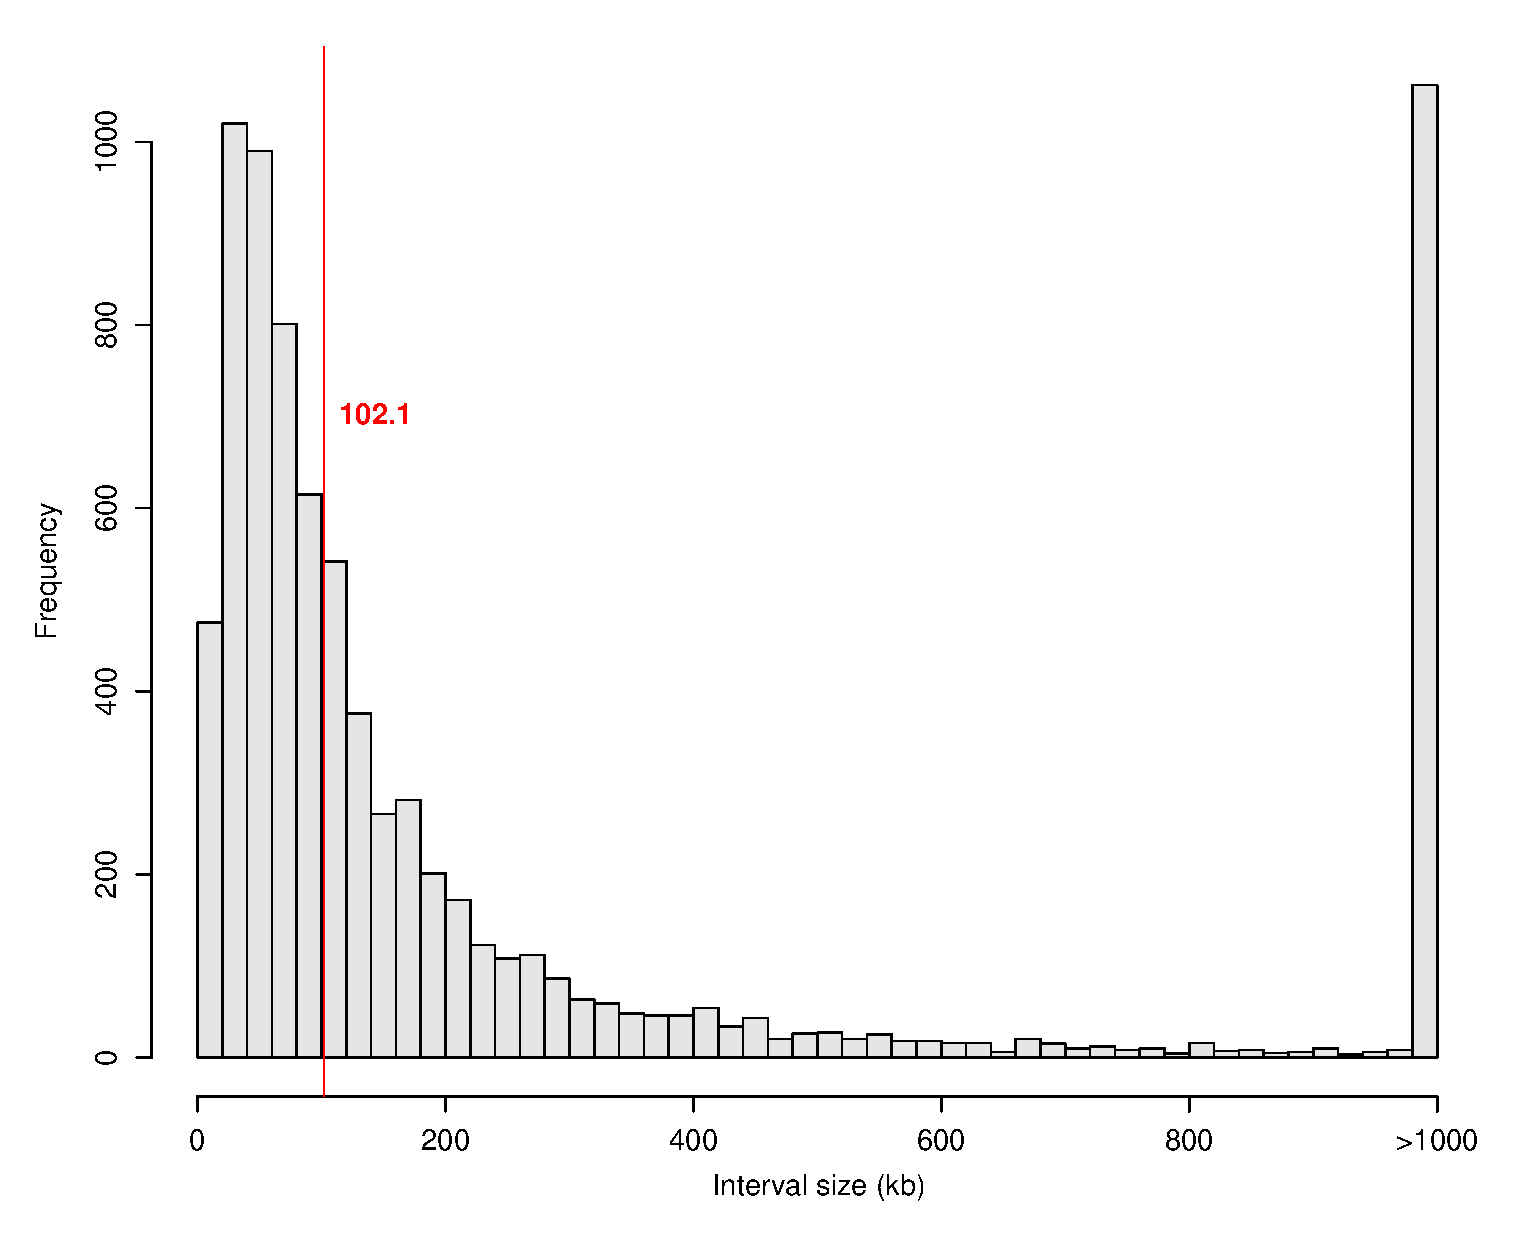
\includegraphics[width=0.5\textwidth]{dogPed/suppfigs/eventWidth_trim_filtered}
    \vspace{-10pt}
    \captionTitle{\textbf{Distribution of crossover interval size.}}{
    The vertical red line represents the median interval size of 102.1 kb.\label{fig:intsize}}
\end{figure}

\begin{figure}[p]
    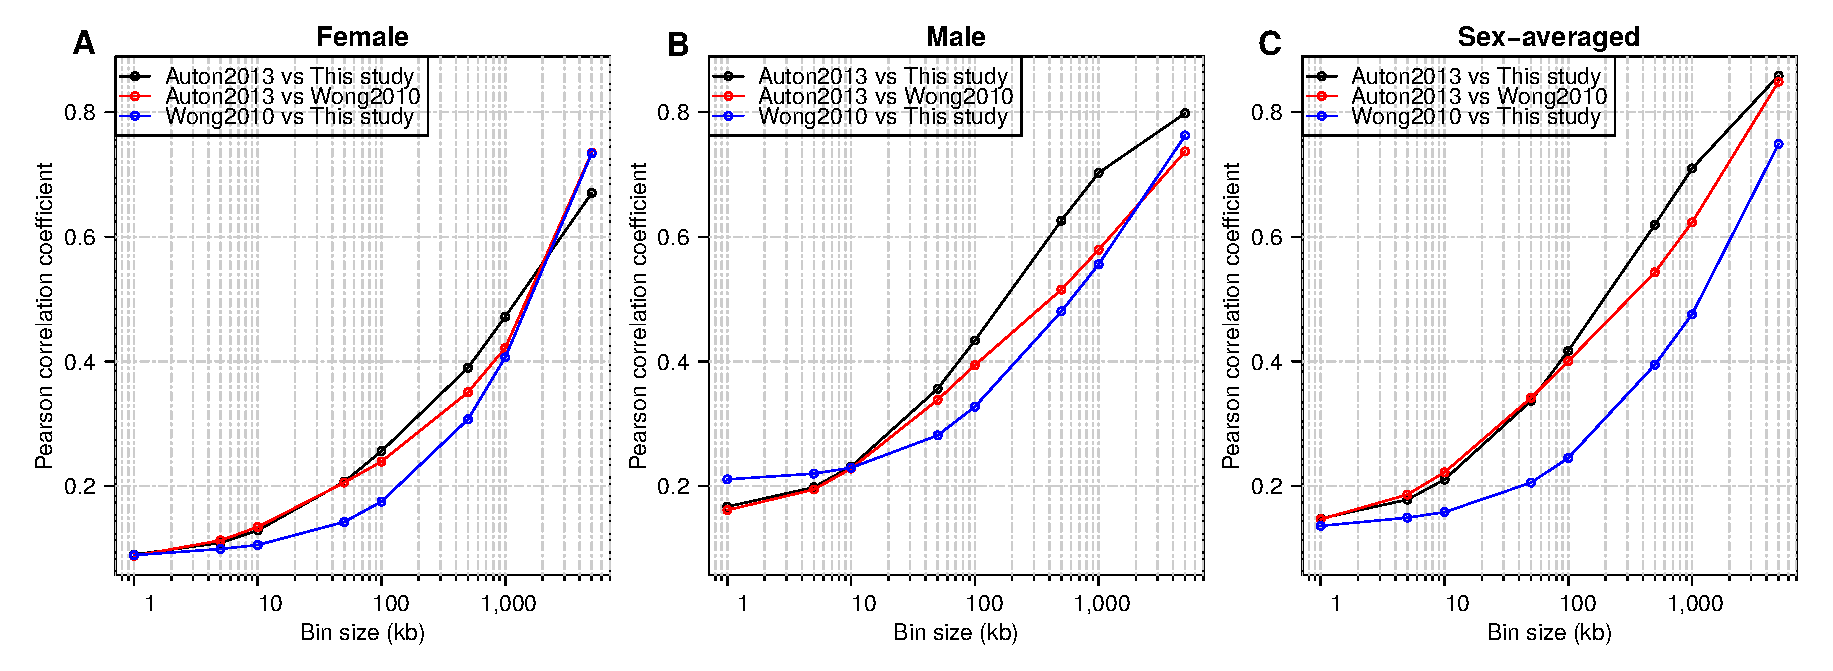
\includegraphics[width=\textwidth]{dogPed/suppfigs/geneticMap_correlations_filtered2}
    \vspace{-20pt}
    \captionTitle{\textbf{Pearson correlation between recombination rates}}{
    estimated from the \citet{Auton2013} LD map, the pedigree maps from \citet{Wong2010}, and this study as a function of scale. \label{fig:mapCor}}
\end{figure}

\begin{figure}[p]
    \includegraphics[width=\textwidth]{dogPed/suppfigs/chr_length_relationship_filtered}
    \vspace{-20pt}
    \captionTitle{\textbf{Map length as a function of physical length for each chromosome}}{
    for female (A), male (B), and sex-averaged (C) maps.  Numbers refer to chromosomes with a linear regression line included.   The sex-specific maps are compared to the \citet{Wong2010} pedigree study, the sex-averaged map is additionally compared to the LD map from \citet{Auton2013} (C, in black). \label{fig:mapLength}}
\end{figure}

\begin{figure}[p]
    \includegraphics[width=\textwidth]{dogPed/suppfigs/recomb_genome_100kb_k50_human}
    \vspace{-20pt}
    \captionTitle{\textbf{Recombination rate across the human genome}}{
    using the 23andMe genetic maps\cite{Campbell2015}. Female rates are shown in shades of red, male rates in blue shades.  Recombination rates were smoothed at the 5 Mb scale. \label{fig:recombRateHuman}}
\end{figure}

\begin{figure}[p]
    \includegraphics[width=\textwidth]{dogPed/suppfigs/8020plot_supplement}
    \vspace{-15pt}
    \captionTitle{\textbf{SNP density affects the proportion of recombination occupying various proportions of the sequence.}}{
        (A) Human data is shown prior to thinning, alongside data from dogs.  Even without thinning in humans, dogs have a more concentrated distribution of recombination.
        (B) Dog data is shown with the thinned human data.  Here, the most telomeric 15\% (by physical distance) of each chromosome arm has been excluded for both species.  Dog recombination remains more concentrated than humans, although the female and male dog curves have flipped at the 80\% recombination mark, likely as a result of the removal of large amounts of telomeric recombination in males.
        (C) The effects of thinning the SNP framework used to create the genetic maps for the human data. Each curve represents a different marker density, from 300,000 SNPs (red line), to 10,000 (blue line).  Reducing the SNP density moves the curve closer to unity and causes recombination to appear to be more spread out throughout the genome. 
        (D) A reduced set of human and dog data are shown with the chromosome sizes approximately matching.
        Each dog chromosome was paired with a corresponding human chromosome arm of a similar size (within 30 Mb).
        This plot includes dog chromosomes 1 through 28; the remainder were too small to have potential matching human chromosome arms.
    \label{fig:8020supp}}
    \end{figure}

\begin{figure}[p]
    \includegraphics[width=\textwidth]{dogPed/suppfigs/rr_around_TSS-CpG}
    \vspace{-20pt}
    \captionTitle{\textbf{Sex differences in recombination}}{
    around the TSS (A) and CpG islands (B). Female rates are shown red, male in blue.  LD-based estimates\cite{Auton2013} are shown in black.  Recombination rates were estimated in 10 kb windows. \label{fig:genomicFeatures}}
\end{figure}

\begin{figure}[p]
    \includegraphics[width=\textwidth]{dogPed/suppfigs/rr_around_TSS-CpG_split}
    \vspace{-15pt}
    \captionTitle{\textbf{Recombination around TSS and CpG islands partitioned by chromosome position.}}{ 
    Male rates are in blue, female in red, rates from the LD map in black. Rates were estimated in 10 kb bins.  Rates were estimated for each feature by taking the centromeric 75\% (A and C) and telomeric 25\% (B and D) of each chromosome separately. \label{fig:TSScpgSplit}}
\end{figure}

\begin{figure}[p]
    \centering
    \includegraphics[width=0.6\textwidth]{dogPed/suppfigs/rr_around_CpG_thinned}
    \vspace{-10pt}
    \captionTitle{\textbf{Recombination around a thinned subset of CpG islands.}}{
    Male rates are in blue, female in red, rates from the LD map in black.  Rates were estimated in 10 kb bins.  CpG islands were thinned to a uniform distribution by keeping a maximum of 5 per non-overlapping 500 kb window. \label{fig:cpgThinned}}
\end{figure}

\clearpage

\begin{figure}[p]
    \includegraphics[width=\textwidth]{dogPed/suppfigs/rr_around_H3K4me3_splitCpG}
    \vspace{-20pt}
    \captionTitle{\textbf{Recombination rate around H3K4 trimethylation marks found in dog spermatocytes of varying stages}}{ 
        Male rates are shown in blue, female in red, and rates from the LD-based map in black.
        %The left column of plots shows peaks in early stages of meiosis (leptotene/zygotene, n=28,303), the middle column pachytene (n=32,718), and the right column the union of all peaks (n=61,021).
        The left column of plots shows peaks in early stages of meiosis (leptotene/zygotene), the middle column pachytene, and the right column the union of all peaks.
        Similarly, the top row includes all peaks, while the middle and bottom rows show peaks with and without overlap with CpG islands, respectively. Rates were estimated in 10 kb bins for all plots.
    \label{fig:H3K4panel}}
\end{figure}

\begin{figure}[p]
    \includegraphics[width=\textwidth]{dogPed/suppfigs/interferenceParameters_byAge}
    \vspace{-20pt}
    \captionTitle{\textbf{Estimates of crossover interference parameters in the dog genome as a function of age.}}{
       Dog meioses were partitioned into 7 approximately equal sized bins on the basis of parental age at birth.
       Interference strength for the simple gamma model is shown in A.
       The parameters for the Housworth-Stahl gamma-escape model are shown in B (interference strength) and C (escape).
       Males are shown in blue and females in red.
       The error bars represent a 95\% confidence interval estimated from 100 bootstrap iterations. \label{fig:cointGenomeAge}}
\end{figure}

\begin{figure}[p]
    \includegraphics[width=\textwidth]{dogPed/suppfigs/interferenceParameters_genome_thinned}
    \vspace{-20pt}
    \captionTitle{\textbf{Estimates of crossover interference parameters in the human genome.}}{
       Here, the human data is thinned according to the procedure outlined in the Methods section, reducing the meiosis count and number of SNPs to more closely resemble what is found in dogs.
       Interference strength for the simple gamma model is shown in A.
       The parameters for the Housworth-Stahl gamma-escape model are shown in B (interference strength) and C (escape).
       Males are shown in blue and females in red.
       Estimates for the full resolution human data are shown in boxes, and the thinned human data in triangles.
       The error bars represent a 95\% confidence interval estimated from 1000 bootstrap iterations. \label{fig:cointGenomeThin}}
\end{figure}

\beginmain


%%%%%%%%%%%%%%%%%%%%%%%%%%%%%%
\begin{SingleSpace}
\chapter{Detection of gene conversion in human admixed population genetic data} \label{ch:geneConv}
%\chapter[Detection of gene conversion]{Detection of gene conversion in admixed population genetic data}
%%%%%%%%%%%%%%%%%%%%%%%%%%%%%%

\noindent Christopher L. Campbell$^1$ and Adam Auton$^{1*}$

\vspace{0.5cm}
\noindent This chapter contains unpublished data.\\

\vspace{0.5cm}
\noindent $^1$ Department of Genetics, Albert Einstein College of Medicine, 1301 Morris Park Avenue, Bronx, New York 10461, USA. \\
\noindent $^*$ Former affiliation.
\end{SingleSpace}


%%%%%%%%%%%%%%%%%%%%%%%%%%%%%%%%%%%%%%%%
%%%%%%%%%%%%%%%%%%%%%%%%%%%%%%%%%%%%%%%%
\section{Introduction}
%%%%%%%%%%%%%%%%%%%%%%%%%%%%%%%%%%%%%%%%
%%%%%%%%%%%%%%%%%%%%%%%%%%%%%%%%%%%%%%%%

%%% Intro & CO/GC description:
Recombination is a fundamental component of meiotic cell division, and the reshuffling of genetic variation has important evolutionary implications, enabling the action of natural selection.
DNA double strand breaks (DSBs) resolve to one of two possible outcomes: crossover (CO) and non-crossover, or gene conversion (GC).
Most research to date has been focused on the large-scale chromosomal exchanges that accompany CO, which are easily detected with a variety of direct and indirect methods.
In contrast, gene conversion (GC), is a non-reciprocal process in which short segments of DNA are transferred from one parental chromosome to another.

Molecular studies support a model in which DNA DSBs occur at multiple points along a chromosome, and each of these DSBs undergoes a repair procedure that results in either CO or GC\cite{}. % Baudat2007?
Sperm typing studies have estimated that GC occurs approximately ten times more frequently than crossover\cite{Jeffreys2004,Baudat2007,Cole2012}.
Gene conversion events are small, typically under 1000 bp\cite{}, but other estimates range from 50-2000 bp\cite{}.
This small size therefore makes GC events difficult to detect using genome-wide inference methods such as pedigree studies or LD analysis.

Despite this, a recent study used SNP array data from multiple three-generation pedigrees to identify $\sim$100 GC events in humans\cite{Williams2015}. 
Supporting results from molecular studies, gene conversions were found to occupy 100-1000 bp tracts.
However, GC events were found to cluster unexpectedly, raising questions as to potential differences in the repair mechanism.


% biased gene conversion
Gene conversion has been also shown to be biased in the exchange of alleles\cite{}.
When occurring around a heterozygous SNP, GC can result in the non-Mendelian transfer of alleles, with the donor allele copied in a 3:1 ratio over the allele on the recipient chromosome.
Furthermore, the copied allele is not chosen completely at random, and there is a dependency in which certain alleles are favored over others.
Weak alleles (A and T) tend to be replaced with strong alleles (G and C). % Duret et al., 2006; Duret and Galtier, 2009; Webster and Hurst, 2012)
This is know as GC biased gene conversion (gcBGC), the over-transmission of G and C alleles during recombination.
Biased gene conversion has evolutionary implications, and has contributed to an ongoing change on the base content of the genome\cite{Bherer2014}.

Several statistical approaches have been proposed to create a model with which to detect gene conversion events from population genetic data.
\citet{Gay2007} created a hidden Markov model (HMM) that models gene conversion together with crossover.
This model was based upon a previous method for detecting recombination using patterns of LD, which modeled haplotype segments as a copied mosaic of previously observed haplotypes\cite{Li2003}.
Another model, although it does not explicitly model gene conversion, is HAPMIX\cite{Price2009}, which adapts the Li and Stephens model to perform ancestry deconvolution on admixed genomes.
In this model, two divergent populations of haplotypes serve as a reference, and the admixed haplotype can copy from either population, with cross-population switches reflecting a change in haplotype ancestry.
HAPMIX has been demonstrated to have a high sensitivity for partitioning admixed genomes\cite{Price2009}.

The HAPMIX approach highlights a relatively new method of studying recombination in human populations having recent admixture.
In this method, an admixed genome is modeled as a mosaic of haplotypes from two ancestral reference populations that have divergent patterns of allele frequencies (Figure \ref{fig:GCadmixture}).
This technique was recently used to study recombination in African American populations\cite{Hinch2011}.
This study found further evidence of population-specific hotspots, finding 2,500 hotspots unique to West Africans, and finding that these are tied to a novel PRDM9 binding motif.


\afterpage{
\begin{figure}[P]
    \includegraphics[width=\textwidth]{geneConv/figs/admix_HMM.png} \vspace{-10pt}
    \captionTitle{\textbf{Admixture approach to gene conversion detection.}}{
        (\textbf{A}) An admixed genome is shown (center) as a mixture of genomic segments from two divergent ancestral populations.
        (\textbf{B}) Diagram showing haplotypes in our HMM.
        Each horizontal line is a haplotype and each column of circles represents the alleles of a SNP, with blue and red colors designating alleles that are representative of two divergent ancestral reference populations.
        The haplotypes for the reference populations are used as templates for the admixed haplotype (bottom). %, in which the alleles are of unknown ancestry.
        The state path of haplotype transitions ($X$) is shown by open circles.
        The gene conversion state path ($G$) is shown in open diamonds.
        In this example there is one gene conversion event at SNP 6 in the admixed haplotype, which is copied from a haplotype in population 1.
        In all other SNPs there is no gene conversion ($G=0$).
        \label{fig:GCadmixture} } 
\end{figure}
\clearpage}
%%%

Here, we will combine key features from each of these two models to develop a new method to detect gene conversion.
Our method aims to detect gene conversion events using admixed population genetic data, where a gene conversion from on population will be detectable with increased contrast against the background of the other divergent population.
From HAPMIX, we use the convention of modeling recombination separately both prior to, and after a point admixture event.
From the \citet{Gay2007} model, we model crossover and gene conversion with independent Markov chains.
Using a combination of these two methods, our model will provide a novel method to detect gene conversion events in humans using admixed genomes.


%%%%%%%%%%%%%%%%%%%%%%%%%%%%%%%%%%%%%%%%
%%%%%%%%%%%%%%%%%%%%%%%%%%%%%%%%%%%%%%%%
\section{Methods}
%%%%%%%%%%%%%%%%%%%%%%%%%%%%%%%%%%%%%%%%
%%%%%%%%%%%%%%%%%%%%%%%%%%%%%%%%%%%%%%%%

% $ \Pr( h_{j+1} | h_1, \ldots, k_j, \rho, \gamma ) $

We provide here details of the implementation on the hidden Markov model used.
We build upon the hidden Markov model framework put forth by \citet{Li2003}, in which an unknown haplotype is modeled as an imperfect mosaic of previously observed haplotypes.
We adopt features from several extensions of this framework that have been used to address population genetics problems in recent years.
The HAPMIX model\cite{Price2009} has been used successfully in the deconvolution of admixed genomes.
In HAPMIX, the Li and Stephens model is modified to include two separate groups of reference populations, corresponding to ancestral populations, from which segements of an unknown admixed haplotype can be assigned.
The Li and Stephens model has also been modified for the detection of gene conversion events, which can be achieved by modeling gene conversion and crossover events simultaneously\citep{Gay2007}.

Here, we take key elements from each of these models: from HAPMIX the use of two divergent reference populations to increase contrast in ancestry, and from the \citet{Gay2007} model the addition of a second Markov chain to model gene conversion events.
Using the ancestry deconvolution approach we can assign blocks of sequence to one ancestral population or the other.
In a block of sequence assigned to one ancestral population, gene conversion events from the other population will stand out against this background, and enable more accurate identification of these events.

\subsection{Model details}
We model gene conversion events along with haplotype transitions (crossovers) as independent Markov processes with transitions possible between each.
In our model an admixed haplotype is composed of an imperfect mosaic of haplotypes from two ancestral populations, labeled $P_1$ and $P_2$, containing $n_1$ and $n_2$ haplotypes, respectively.
We assume that the unknown, admixed haplotype underwent a point admixture event $T$ generations in the past,
in which a proportion, $\mu_1$, of that haplotype's ancestry comes from $P_1$, with the remainder, $\mu_2 = 1-\mu_1$, contributed from $P_2$.

The crossover chain is affected by both ancient and recent crossover events.
Ancient events are controlled by the population crossover rate, $\rho = 4 N_e r$, where $N_e$ is the effective population size and $r$ is the per-generation recombination rate.
From HAPMIX, recent recombination events are modeled by considering the per generation recombination rate, $r$, and the estimated time since the admixture event, $T$.
This $T$ parameter allows the per generation recombination rate to be scaled to account only for recent events, and model specifically switches in ancestry.
The $\rho$ parameter is allowed to vary across regions tested in our model, and we use a genetic map to obtain the recombination rate $r$.

From the \citet{Gay2007} model, the gene conversion chain is modeled similarly, with the frequency of gene conversion affected by the population gene conversion rate $\gamma = 4 N_e g$, where $g$ is the per-generation gene conversion rate.
%However, we we do not attempt to capture events that occurred previous to the admixture event, and we thus omit the population scaled gene conversion rate,
We the HAPMIX convention of modeling recent events using the per-generation gene conversion rate, $g_j$ and the time since admixture, $T$.
At the same time, we model ancient gene conversion events, prior to admixture, using the $\gamma$ parameter.

% our HMM consists of terms, $\Pr(h_1,\ldots,h_{(n_1+n_2)},\rho_1,\rho_2,\gamma_1,\gamma_2)$.
Our HMM has $(n_1+n_2)+(n_1+n_2)^2$ possible states, where $X_j$ represents the parental haplotype copied at site $j$ and $G_j$ represents the gene conversion state at site $j$.

\paragraph*{Parameter settings.}
We use two divergent reference populations, arbitrarily labeled.
The first, population $P_1$, will be used to represent Europeans, while the second, $P_2$, will represent a population of African origin.
We take into account the differences in effective population size, $N_e$, by setting $N_{e1} = 10,000$ and $N_{e2} = 18,000$.
The population sizes translate to differences in the population recombination and gene conversion parameters for each population, giving $\rho_1$, $\rho_2$, $\gamma_1$, and $\gamma_2$.
We use the Hapmap2 genetic map\cite{hapmap2007} to obtain the recombination rate between pairs of sites.
We set $T$ to be 7 generations, and assume the ancestry contribution from Europeans, $\mu_1$, is 0.2.
We set the ratio between gene conversion and crossover rate, $f = g / r = 10$, based on estimates previously made using sperm typing\cite{Jeffreys2004} and population genetic\cite{Gay2007} data.
The expected length of a gene conversion tract, $1/\lambda$, is fixed at 500bp.

\subsection{Transition probabilities}
Following \citet{Gay2007}, the transition probabilities for crossover ($X$) and gene conversion ($G$) chains occur simultaneously.
The crossover chain is independent and depends only upon the previous state within its own chain.
However, it was necessary to consider gene conversion in the context of the current population of the crossover chain because our approach relies on the detection of gene conversion events that are copied from a different population from the haplotype as a whole.
Therefore, we make a modification to the transition probabilities of the gene conversion chain:
%
\begin{equation} \Pr(X_{j+1}, G_{j+1} | X_{j},G_{j} ) = \Pr(X_{j+1}|X_{j}) \Pr(G_{j+1}|G_{j},X_{j}) ~. \end{equation}

For each site we consider the transition from one haplotype to another, taking into account population specific parameters for $\rho$, $\gamma$, $\mu$, and $n$.
If the destination haplotype belongs to $P_1$ we use $\rho_1$, $\gamma_1$, $\mu_1$ and $n_1$; for haplotypes transitioning into $P_2$, $\rho_2$, $\gamma_2$, $\mu_2 = 1-\mu_1$, and $n_2$.
%We consider the possibility of switching between the two parental populations, and we label the source (previous) population $p_k$ and the destination population (at site $j+1$) $p_l$.
The population containing the haplotype at site $j$ is labeled $p_k$, and the population that contains the destination haplotype, at site $j+1$, is labeled $p_l$.


\subsubsection*{Starting probabilities}
%%%
% The probability of the crossover chain starting in any given haplotype is scaled by the estimated ancestry contribution ($\mu$) from each population to the admixed haplotype:
There is an equal probability of starting the crossover chain in any given haplotype, scaled by the estimated ancestry contribution ($\mu$) from each population to the admixed haplotype, where $x \in p_l$:
\begin{equation} \Pr(X_1 = x) = 
        \mu_l/n_l ~.
%\begin{dcases}
%        %\mu_1/n_1 & \text{if $x \in p_1$} \\
%        %(1-\mu_1) /n_2 & \text{if $x \in p_2$} ~.
%\end{dcases}
\end{equation}
%%%
The gene conversion chain can start either within or outside of a gene conversion state.
For the null state we consider the possibility of having ended a gene conversion tract from any of the haplotypes, and the estimated rate of gene conversion since admixture.
The gene conversion chain can also start within a haplotype in each of our two reference populations, dependent on the expected rate of gene conversion since admixture and weighting the haplotypes of each population by the ancestry contribution, $\mu$, to the admixed haplotype.
%The parameter $\mu$ is used to weight the number of haplotypes by their expected ancestry contribution to the admixed haplotype.
Since we have no information outside this first site, we set the value of $g = f r$, where we use the estimated genome-wide recombination rate of 1.1 cM/Mb for $r$.
\begin{equation} 
\Pr(G_1 = g) =  \\
\begin{dcases}
    \frac{\lambda (n_1+n_2) }{ \lambda (n_1+n_2) + g T }
& \text{if $g = 0$} \\
    \frac{ g  T }{ \lambda (n_1+n_2) + g T } \frac{\mu_l}{n_l}
& \text{if $g \ne 0$ and $g \in p_l$} \\
\end{dcases}
\end{equation}


%%%%%%%%%%%%%%%%%%%%%%%%%%%%%%%%%%%%%%%%%%%%%%%%%%
%%%%%%%%%%% X transitions
%%%%%%%%%%%%%%%%%%%%%%%%%%%%%%%%%%%%%%%%%%%%%%%%%%

\subsubsection*{Crossover transition probabilities}
The probability of transitioning from a hidden state at site $j$ to a hidden state at site $j+1$ depends on several parameters,
including the physical distance $d_j$ (in base pairs) and recombination rate, $r_j$ (e.g., cM/Mb).
We adopt the approach used by HAPMIX to capture recent crossovers since admixture as a product of the per-generation genetic distance between markers, $r_j d_j$, and the number of generations since admixture, $T$.
Ancient recombination is modeled using the population scaled recombination rate, $\rho$, scaled by the number of haplotypes in the population.
Each population has its own $\rho$ parameter, which depends on the effective population size.
%
\begin{multline}
     \Pr(X_{j+1}=x' | X_{j}=x) = \\
\begin{cases}
%\displaystyle 
\hfill   (1-e^{-r_j d_j T}) \frac{\mu_l}{n_l}  
        &  \text{if $x \ne x'$ and $p_k \ne p_l$ } \\
%\displaystyle     
\hfill e^{-r_j d_j T} (1-e^{-\rho_{l,j} d_j / n_l }) \frac{1}{n_l} + 
        (1-e^{-r_j d_j T}) \frac{\mu_l}{n_l}  
        &  \text{if $x \ne x'$ and $p_k = p_l$ } \\
%\displaystyle 
        e^{-r_j d_j T} e^{-\rho_{l,j} d_j / n_l } +
        e^{-r_j d_j T} (1-e^{-\rho_{l,j} d_j / n_l }) \frac{1}{n_l} + 
        (1-e^{-r_j d_j T}) \frac{\mu_l}{n_l}
        &  \text{if $x=x'$ and $p_k = p_l$ } \\
        %
\end{cases}
\end{multline}

%%%%%%%%%%%%%%%%%%%%%%%%%%%%%%%%%%%%%%%%%%%%%%%%%%
%%%%%%%%%%% G transitions
%%%%%%%%%%%%%%%%%%%%%%%%%%%%%%%%%%%%%%%%%%%%%%%%%%

\subsubsection*{Gene conversion transition probabilities}
Here we follow the \citet{Gay2007} model with modifications to account for the two ancestral populations and switches between them, focusing on identifying the recent events since admixture.
In the case where $X_j$ and $G_j$ occur within the same population, we must account for gene conversions occurring both prior to, and since the admixture event.
The population scaled rate, $\gamma$, is used to model gene conversion events occurring prior to admixture.
For gene conversions occurring after the admixture event, we use the HAPMIX convention, as in the crossover transitions, of modeling recent gene conversion events by the per generation gene conversion rate, $g$, and the number of generations since admixture, $T$.
We are specifically interested in capturing the situation in which $X_j$ and $G_j$ occur across different populations.
In this case, we do not model ancient events, but focus on capturing only recent gene conversions.

Generally, the probability of both starting a gene conversion and ending one within the interval is taken into account to determine $\Pr(G_{j+1}|G_j,X_j)$.
The rate of ending a gene conversion tract, $\lambda$, is modeled geometrically as a function of physical distance.
This allows allowing termination to occur at any point within the interval and for the tract to ``reset'' at any time regardless of the current state. %%% fix this
The probability of starting a gene conversion event is given by the product of $g$ and the number of generations since admixture, $T$.
%We expand the \citet{Gay2007} model to include two independent $\gamma$ parameters, one for each population.



\paragraph{The gene conversion null state.}
In the first transition, we move from a null gene conversion state ($G_j=0$) to another null gene conversion state ($G_{j+1}=0$).
This is given by the probability of having no reset event and no gene conversion event in the interval, either prior to, or after admixture.
%
\begin{equation} \label{eq:Gnull}
    \begin{split}
        \Pr(G_{j+1}=0|G_{j}=0,X_j=x) = \\
        e^{-\lambda d_j} e^{-g_j d_j T } e^{-d_j \gamma_l/n_l} +
    \int_0^{d_j} \lambda e^{-\lambda x} e^{-g_j x T } e^{-x \gamma_l/n_l } ~\mathrm{d}x ~~~
     \text{if $x \in p_l $ } \\%[1em]
\end{split}
\end{equation}
%
The integral represents the possibility that there was a reset event, but no gene conversion event.

\paragraph{Entering a gene conversion event}
The second transition describes the probability of entering a gene conversion state from a null state.
When $g$ and $x$ are within the same population, we must account for gene conversions events occurring prior to admixture, as well as those occurring after.
We use the following constant, $Z$, to scale the gene conversion rate.
The left term accounts for the post-admixture gene conversion rate, $g_j T$, scaled by $u_l/n_l$ for the target population.
The right term captures events occurring prior to admixture, using the population scaled gene conversion rate $\gamma_l/n_l$.
\newcommand{\constZ}{\bigg[ \frac{g_j T}{g_j T + \gamma_l/n_l} \mu_l + \frac{\gamma_l/n_l}{g_j T + \gamma_l/n_l}  \bigg] \frac{1}{n_l} }
\begin{equation} \label{eq:constZ}
    Z = \constZ
\end{equation}

For the transition, we consider case in which there has been no reset, but a gene conversion event has taken place prior to or after $T$.
We also account for the case (within the integral) in which there was a reset event, with a gene conversion event taking place afterwards.
The population from which the gene conversion chain now copies is taken into account within the gene conversion term using $\mu_l$ for the ancestry proportion for $p_l$, where $g \in p_l$:
%
\begin{equation} 
\begin{split}
    \Pr(G_{j+1}=g|G_{j}=0,X_j=x) =  \\
\begin{dcases}
    e^{-\lambda d_j} (1-e^{-g_j d_j T - d_j \gamma_l / n_l}) Z +  \\
    \int_0^{d_j} \lambda e^{-\lambda x} (1-e^{-g_j x T -x \gamma_l / n_l }) Z ~\mathrm{d}x
    &  \text{if $g \in p_l $ and $x \in p_l $ } \\%[1em]
e^{-\lambda d_j} (1-e^{-g_j d_j T }) \frac{\mu_l}{n_l} +  
\int_0^{d_j} \lambda e^{-\lambda x} (1-e^{-g_j x T }) \frac{\mu_l}{n_l} ~\mathrm{d}x
    &  \text{if $g \in p_l $ and $x \not\in p_l $ } \\%[1em]
%%%
\end{dcases}
\end{split}
\end{equation}

\paragraph{Ending a gene conversion event.}
In the third case, we describe the probability of ending a gene conversion within the interval.  
% Here, there has been a reset event with no gene conversion following.
As in \eqref{eq:Gnull}, we are transitioning into a null gene conversion state and the population information is taken from the $X$ chain:
%
\begin{equation}
    \Pr(G_{j+1}=0|G_{j}=g,X_j=x) = 
    \int_0^{d_j} \lambda e^{-\lambda x} e^{-g_j x T } e^{-x \gamma_l/n_l} ~\mathrm{d}x ~~~
     \text{if $x \in p_l $ } \\%[1em]
\end{equation}


\paragraph{Continuing a gene conversion event.}
Finally, we consider the case where we transition from a gene conversion state to another gene conversion state.
In the situation where $g=g'$ we are simply continuing to copy from the same haplotype in the same gene conversion event.
This is given by the probability of having no reset event, or having a reset, and then a gene conversion back to the same haplotype.
When $g \ne g'$ we are transitioning from a gene conversion state in one haplotype to a different gene conversion in a different haplotype (an overlapping gene conversion).
Within this interval we have a reset event followed a gene conversion event to a different haplotype, potentially in a different parental population:
%
%\begin{multline}
\begin{equation} \begin{split}
\Pr(G_{j+1}=g'|G_{j}=g,X_j=x) = \\
\begin{dcases}
    % extend a gene conversion within the same population
    e^{-\lambda d_{j}} + 
    \int_0^{d_j} \lambda e^{-\lambda x} (1-e^{-g_j x T -x\gamma_l/n_l}) Z ~\mathrm{d}x
    &  \text{if $g = g'$ and $g' \in p_l $ and $x \in p_l$ } \\%[1em]
%%%
    e^{-\lambda d_{j}} + 
    \int_0^{d_j} \lambda e^{-\lambda x} (1-e^{-g_j x T }) \frac{\mu_l}{n_l} ~\mathrm{d}x
    &  \text{if $g = g'$ and $g' \in p_l $ and $x \not\in p_l$ } \\%[1em]
%%%
    \int_0^{d_j} \lambda e^{-\lambda x} (1-e^{-g_j x T -x\gamma_l/n_l}) Z ~\mathrm{d}x
    &  \text{if $g \ne g'$ and $g' \in p_l $ and $x \in p_l$ } \\%[1em]
%%%
    \int_0^{d_j} \lambda e^{-\lambda x} (1-e^{-g_j x T }) \frac{\mu_l}{n_l} ~\mathrm{d}x
    &  \text{if $g \ne g'$ and $g' \in p_l $ and $x \not\in p_l$ } \\%[1em]
\end{dcases}
%\end{multline}
\end{split}
\end{equation}


\subsection{Emission probabilities.}
%We allow for errors in the copying chain by using mutation parameters proportional to the number of haplotypes in each population, as in HAPMIX\cite{Price2009}:
We allow for errors in the copying chain with a mutation rate defined using Watterson's estimator\cite{Watterson1975,Li2003}.
We use a separate $\theta$ for each population:
%
\begin{equation}
    \theta_l = \Bigg( \sum\limits_{m=1}^{n_l-1} \frac{1}{m} \Bigg) ^{-1} ~.
\end{equation}

We then follow the Li and Stephens model to calculate the emission probability at site $j$ for the unknown admixed haplotype, $a$, conditional on the underlying hidden state ($X_j,G_j$).
We compare the haplotype from which we are copying, $c$, where $c=X_j$ if $G_j=0$, else $c=G_j$:
\begin{equation}
    e_a(j|X_j,G_j) = \\
    \begin{dcases}
        \frac{ \theta_l }{ 2 (n_l+\theta_l ) }          & \text{if $h_{a,j} \ne h_{c,j}$ and $h_{c,j} \in p_l$ } \\
        \frac{ 2 n_l + \theta_l }{ 2(n_l+\theta_l) }    & \text{if $h_{a,j} = h_{c,j}$ and $h_{c,j} \in p_l$ } ~.
    \end{dcases}
\end{equation}



\subsection{Computational Efficiency}
\paragraph{HMM state space.}
Given the large number of states in our model ($(n_1+n_2)$ for the crossover chain, plus $(n_1+n_2)^2$ for the gene conversion chain), increasing the number of haplotypes in the reference populations quickly produces an excess of states at each site, most with very low probability.
Using just 100 reference haplotypes requires 10,100 states, while increasing this number to 400 produces 160,400 states for each site (Figure \ref{fig:GCnStates}).
Computation using the forward-backward algorithm on even the highest performance modern processors is infeasible for even a modest number of sites.
It is important to have a large enough population of reference haplotypes, in order to avoid incomplete capturing of diversity in the reference population, and provide a close enough match to each segment in the unknown admixed sample.
Considering the availability of public data from the Hapmap\cite{hapmap2007} and 1000 Genomes projects\cite{1000G2015} we set a target of approximately 200 phased haplotypes in each reference population.
%%%
\afterpage{
\begin{figure}[P]
    \begin{center}
    \includegraphics[width=\textwidth]{geneConv/figs/nStates}
    \end{center} 
    %\vspace{-20pt}
    \captionTitle{\textbf{Complexity of the gene conversion model.}}{
        The number of states is shown as a function of the total number of reference haplotypes.
        For a small number of haplotypes (50 in each reference population), there are 10,100 states.
        With 200 haplotypes in each population this increases to 160,400 states.
    \label{fig:GCnStates}} 
\end{figure}
\clearpage}

\paragraph*{Two-pass approach.}
To reduce the computation time for this model, we apply a two-pass approach.
In the first pass, we use only the crossover chain, and omit all gene conversion states from the model, reducing the number of states to ($n_1+n_2$).
The mutation parameters for both populations, which allow for a degree of copying error in the Markov chain, are set to approximately 0 (equivalent to machine epsilon).
This configuration forces the most likely state path (calculated using the Viterbi algorithm) to make a switch at each point a mismatch is detected between the copying haplotype and the unknown admixed haplotype (Figure \ref{fig:GCtwoPassSchematic}A).

Using this no-error Viterbi path, we identify long stretches (greater than 14 sites) where the admixed haplotype matches exactly to a reference haplotype.
These long stretches are likely to represent evolutionarily conserved shared haplotype segments.
Since our goal is to detect gene conversion events from one ancestral population against the background of the other population, these long stretches are unlikely to contain any information of interest (and this is supported by a lack of gene conversion events in our simulation).  
Instead, we look for regions where the Viterbi path makes short jumps between haplotypes of different reference populations, indicating a perfectly matching stretch of haplotype was not present in the reference.
These clusters of haplotype switches represent potential regions in which cross-population gene conversion events (or crossover) have disrupted linkage between neighboring sites.
We select haplotype stretches in the no-error Viterbi path that are short ($\le 14$ sites), and make a cross-population switch in haplotypes. % ([then back again?]).
For each of these stretches identified we select an additional 3 sites on each side of the stretch to capture events that may have occurred at the beginning or end.

We then make a second pass through the data, making a deeper inspection of the stretches of contiguous sites marked in the first pass though the data (Figure \ref{fig:GCtwoPassSchematic}B).
%Here the full HMM, with both crossover and gene conversion chains, is run only on only the sites that passed the criteria in the first pass.
Here the HMM is run using only the crossover chain (as in the first pass), except at sites marked for deeper inspection.
At these sites the gene conversion chain is turned on and we allow all possible transitions under the full HMM.
This technique allows a drastic reduction in the model complexity at sites that are unlikely to contain a gene conversion event (or at least those that are able to be detected by our model).
%%%
\afterpage{
\begin{figure}[P]
    \begin{center}
    \includegraphics[width=\textwidth]{geneConv/figs/schematic_2pass.png}
    \end{center} 
    %\vspace{-20pt}
    \captionTitle{\textbf{Schematic of the two-pass HMM approach.}}{
        Each horizontal line is a haplotype, with blue and red colors designating segments that are representative of two divergent ancestral reference populations.
        Each column of circles represents the alleles of a SNP.
        The state path of haplotype transitions ($X$) is shown by open circles while the gene conversion state path ($G$) is shown in open diamonds.
        In \textbf{A} the gene conversion chain is not used and the crossover chain is forced to jump to $h3$ to accommodate the gene conversion.  
        In \textbf{B} the gene conversion chain is not used except for a few sites on either side of the putative gene conversion event.
    \label{fig:GCtwoPassSchematic}} 
\end{figure}
\clearpage}
%%%

Further reduction in computation time is achieved by running the second pass on smaller subsamples taken from the total body of reference haplotypes.
For example, with a group of 200 haplotypes in each reference population, we draw 10 random samples of 50 haplotypes from each.
We then run the reduced complexity model on the 10 subsets.
Finally, the results from each of the subsets are combined by taking the mean posterior probability of a cross-population gene conversion event.
This allows a drastic reduction in the number of total states, and thus a much faster run time.


\subsection{Simulation}
In order to test the ability of the model to identify gene conversion events, we first evaluate its performance using simulated data where the true GC events are known.
Data from the 1000 Genomes Project (Phase III\cite{1000G2015}) serves as source data from which we draw haplotypes for our parental populations.

Since our model attempts to infer recombination rates, the use of data 1000 Genomes data that was assembled and phased using a genetic map (the Hapmap phase II map\cite{hapmap2007}) would introduce a potential bias.
In order to avoid this bias, we first re-phase the data.
We use SHAPEIT\cite{Delaneau2013} to construct phased haplotypes from genotype data.
SHAPEIT requires a genetic map as a prior input for phasing, so we create a map with the same intervals as the standard Hapmap genetic map, but with the recombination rate at each interval set to 1.1 cM/Mb.
In addition, our method uses a genetic map, with estimates of the recombination rate at each site, to provide values for parameters for the per-generation crossover rate, $r$, and by extension, the gene conversion rate, $g$ (which is equal to $f r$).
As this also has the potential to introduce bias, we again use a genetic map with a fixed recombination rate.

To create simulated admixed haplotypes, we use a 1 Mb region on chr22, taking all phased haplotypes from two groups of reference populations.
For Eurpean haplotypes we select CEU, GWR, and TSI populations (n=399), and we select YRI and LWK for African populations (n=302).
We draw 100 haplotypes from each of two reference populations.
SNP density is thinned to keep 300 sites, and singleton variants are removed from the analysis.

An initial point admixture is then simulated for 50 haplotypes by drawing one haplotype from each reference population and creating a recombinant ``offspring'' haplotype.
The number of crossovers is determined by sampling from a Poisson distribution ($r = 1 / \mathrm{Mb}$).
Gene conversions are likewise placed under a Poisson process ($g = 10/1 \mathrm{Mb}$; $1/\lambda = 500 \mathrm{bp}$).
Following the initial admixture event, six subsequent generations were simulated using intra-population mating, with CO and GC events recorded each time they occurred. 
Our HMM is then run using a single haplotype from the simulated admixed population, drawn at random.


%%%%%%%%%%%%%%%%%%%%%%%%%%%%%%%%%%%%%%%%
\section{Results}
%%%%%%%%%%%%%%%%%%%%%%%%%%%%%%%%%%%%%%%%


We test the performance of our model using simulated genomes on real human data from the 1000 Genomes Project\cite{1000G2015}.
Using a small sub-section of chromosome 22, we select parent haplotypes from CEU and YRI populations, representing individuals of European and African descent, respectively.
Recombination crossovers are placed with a rate of 1 / Mb, and gene conversions at 10 times this rate (10 / Mb).
We use a mixing proportion, $\mu$ = 0.5, instead of the 0.8 value estimated from previous methods\cite{Price2009}.
The location and type of each gene conversion is recorded for evaluation purposes.

Gene conversions can be classified into one of three types, based upon how our model will be able to detect them.
We are unable to detect GCs that do not overlap a SNP, and label these ``invisible'' GC events.
GCs that do overlap a heterozygous SNP, and do not produce any change in the alleles are labelled ``silent'' GC events.
Finally, GC events that overlap a SNP and produce a detectable change in the allele are termed ``non-silent'' events, and are the only ones that are detectable by our model.
Therefore, our results only account for non-silent gene conversion events, and we do not consider the other cases, even though they may occur as a result of the simulation.


For all GC events detected, we record the total posterior probability of finding a GC event at that site, and whether this is a real (non-silent) GC event.
Using a threshold of 0.5 for the posterior probability, we estimate the true positive rate at $~$X\%, while the false discovery rate is $~$X\% (Figure \ref{fig:GCperformance}).


\afterpage{
\begin{figure}[P]
\begin{center}
    %\includegraphics[width=\textwidth]{figs/TPR-FDR_NotUsingParentHaps.pdf}
    \end{center} 
    \vspace{-20pt}
    \captionTitle{\textbf{Performance of the model.}}{
    True positive (TPR) false discovery (FDR) rates from simulated data as a function of the threshold on posterior probability of a gene conversion event.
\label{fig:GCperformance} }
\end{figure}
\clearpage}


\section{Discussion}

The detection of recombination within population genetic data using LD based approaches has been used in a number of studies in humans, yielding valuable results\cite{Mcvean2004,Myers2005,hapmap2007}.
A number of methods have been based on a method described by \citet{Li2003} in 2003, in which haplotypes are modeled as a mosaic of segments from other haplotypes.
Several extensions from this method have produced valuable models to detect gene conversion\cite{Gay2007}, and accurately infer admixture breakpoints\cite{Price2009,Hinch2011}.
The admixture approach to recombination is a promising one, especially considering the expanding availability of data on a number of human populations of diverse origins, many of them admixed.

The detection of gene conversion events has long been a difficult problem, owing to their small size, and the confounding effects of genootyping error.
Most studies focus on crossover and ignore the effects of gene conversion, which provides an incomplete picture of the recombination process as a whole.
In our model, the use of admixed genomes provides a unique leverage, in which we detect gene conversion events from one ancestral population against a contrasting background from the other.
In out model, we adopt the Li and Stephens model to include gene conversion, as in \citet{Gay2007}, and two reference populations, as in HAPMIX\cite{Price2009}.
This resulting model attempts to identify cross-population gene conversion events with a higher contrast.

% Simulation results show...

While the complexity of this model is quite high, we have made several advances that allow the computation time to be brought down.
First, we have reduced the state space by dividing the reference populations into ten random subsets.
The model was run on these subsets, and the results combined to generate an approximation to the model under the full set of reference haplotypes.
In addition, we built in the ability to run our model in two parts.
The first pass runs quickly, using only the crossover chain, and screens for potential breakpoints.
In the second pass, full model with both CO and GC chains is used, but only on a subset of the sites that had been previously marked for deeper inspection.
These advances can potentially be generalized to other HMMs of similar structure in the future.
Despite these advances, the complexity is such that it is impractical to run this data on full genomes without significant advances in cputer architecture.

In addition inference using this model, while theoretically possible, is not practical.
Other models use maximum likelihood methods to estimate optimal parameter settings.
In the Li and Stephens model, this technique was used to estimate $\hat{\rho}$ from human data, providing approximations to the recombination rate across the genome.

This model provides a method to detect recombination and gene conversion in admixed population genetic data.
While the complexity of this model is high, it has the potential to be used in human data, especially as the availability of admixed data increases.
% Future work in this area will be necessary to 




%%%%%%%%%%%%%%%%%%%%%%%%%%%%%%%%%%%%%%%%
%%%%%%%%%%%%%%%%%%%%%%%%%%%%%%%%%%%%%%%%
\clearpage
\renewcommand{\bibname}{References}
\bibliographystyle{ccampbell_thesis}
\begingroup
    \setlength{\bibsep}{10pt}
    \linespread{1}\selectfont
    \bibliography{/home/ccampbell/Dropbox/papers/recombination,/home/ccampbell/Dropbox/papers/thesis,/home/ccampbell/Dropbox/papers/GeneConversion}
\endgroup
%%%%%%%%%%%%%%%%%%%%%%%%%%%%%%%%%%%%%%%%
%%%%%%%%%%%%%%%%%%%%%%%%%%%%%%%%%%%%%%%%



%%%%%%%%%%%%%%%%%%%%%%%%%%%%%%
\chapter{Discussion} \label{ch:discussion}
%%%%%%%%%%%%%%%%%%%%%%%%%%%%%%



%%%%%%%%%%%%%%%%%%%%%%%%%%%%%%%%%%%%%%%%
% \section{Characterization of recombination in humans and dogs}
%%%%%%%%%%%%%%%%%%%%%%%%%%%%%%%%%%%%%%%%

In my thesis, I have presented pedigree analyses of meiotic recombination in both humans and dogs.
% In humans, this large scale study contributes to a growing body of research on recombination, and how it differs between males and females.
The 23andMe analysis in humans represents a comprehensive study with a large number of meioses, adding to existing research to further characterize recombination. % and how it differs between males and females.
This study examines sexual dimorphism in recombination, specifically evaluating overall rate distribution, as well as regulatory mechanisms of hotspot usage, and crossover interference.
A major advance from this study was to further characterize maternal age effects on recombination.
These age effects were found to manifest across several aspects of recombination placement, contributing to an overall pattern of deregulation with increased age.

Recombination is not nearly as well characterized in dogs.
However, dogs present a unique species in which to study recombination, largely due to the multiple truncating mutations that have rendered PRDM9 inactive millions of years ago.
The loss of this key recombination regulatory mechanism raises important questions on the role of recombination and specifically how the dog genome has been shaped by recombination in the absence of PRDM9.
The pedigree analysis presented in Chapter \ref{ch:dogPed} represents an important advance towards this goal.
%While the sample size is modest, 
Here, I have shown that dog recombination is similar to humans on a broad scale, with high rates at the telomeric ends being male-driven.
At the fine scale, the lack of PRDM9 is evident in the concentration of recombination at gene promoters, with sex differences that differ from those of humans in some aspects.

In addition, I have developed a statistical model for the detection of gene conversion in human admixed population genetic data.
This model integrates key features of two previous models.
First it leverages the divergence between two distinct reference populations to pick out gene conversion events in admixed population genetic data.
Second, it models gene conversion and crossover simultaneously using two different Markov chains.
Although it is computationally intensive, this model has the potential to advance our understanding of gene conversion and its role within the recombination process.

%%%%%%%%%%%%%%%%%%%%%%%%%%%%%%%%%%%%%%%%
\section{Sex dimorphism in recombination}
%%%%%%%%%%%%%%%%%%%%%%%%%%%%%%%%%%%%%%%%

\subsection{Heterochiasmy}

Heterochiasmy, the difference in recombination rate between the sexes, has been observed in a wide variety of species over the course of decades of studies.
In most studied species, the recombination rate is higher in females, and a number of possible explanations exist to explain this.
Many studies suggest that heterochiasmy is tied to the biological differences in meiosis between the sexes.
Theoretical explanations suggest that natural selection could act to modify recombination rate in either the haploid or diploid life stages.
Since diploid selection is presumably stronger in males, this would contribute to a reduced recombination rate to keep favorable haplotypes in successful males\cite{Trivers1988}.
Selection at the haploid stage is presumed to be restricted to males, since fertilization marks the completion of female meiosis, and there is essentially no haploid phase\cite{Lenormand2005}.
Another possibility is that meiotic drive plays a role in driving evolution of the female recombination rate.
That is, alleles that have an increased probability to be transmitted in oogenesis are more likely to exert selective pressures that modify the female recombination rate\cite{Brandvain2012}.

While unable to address these hypotheses directly, the pedigree data presented in this thesis adds a further data point to the ratio of female to male recombination in humans and dogs; two species separated by millions of years of evolutionary divergence.
In humans, the consensus among many studies over the past decades is that this ratio is approximately 1.6 within the autosomes.
This puts humans among the most heterochiasmate species currently known, although there are a number of studies in amphibians and fish that report much higher ratios (Table \ref{tab:introHeterochiasmy}).

In dogs, I found the ratio to be considerably lower, at 1.2 (Chapter \ref{ch:dogPed}), which matches the ratio reported in a previous dog pedigree study\cite{Wong2010}, both of which studied recombination in purebred dogs.
This indicates that the level of heterochiasmy is not as strong in dogs as it is in humans.
% If we use the hypothesis that selection drives heterochiasmy, then it appears that
Inbred dogs have been subject to strong artificial selection since the creation of modern breeds, and artificial selection has been suggested to have a strong effect on recombination rates.
This suggestion came from a study in domestic cattle, in which a decline in recombination rate was seen over time in response to artificial selection\cite{Ma2015}.
Considering dogs have been subject to extreme artificial selection as well, selection may have played a role in the modification of dog recombination.


\subsection{Hotspot overlap.}

PRDM9 has been shown to undergo rapid evolution within its DNA-binding zinc finger array\cite{Oliver2009,Ponting2011}, and this evolution underlies the lack of sharing between human populations\cite{Hinch2011}, and between species\cite{Auton2012a}.
Previous work in humans found no difference in hotspot usage between male and females\cite{Coop2008}, with the caveat that a relatively small number of meioses was used.
In this thesis, I report for the first time that males have a higher hotspot usage than females, with a difference of 4.6\%.
This difference is not due to the position of hotspots within the genome, nor to recombination rate differences between males and females.

One possible explanation for this is that the set of reference hotspots used was generated from LD studies of recombination\cite{Myers2005,hapmap2007}.
They are therefore a sex-averaged collection, and may be biased in representation of hotspots from males and females.
% These hotspots likely have a population bias, but it is unknown whether there is a sex bias.
Given that females have a greater number of dimorphic regions of recombination than males (Appendix A, \citet{Bherer2016}), it is plausible that there are a greater number of female hotspots, resulting in a more diffuse hotspot usage per individual.
While it is currently not possible to answer this question, future expansions to pedigree studies will provide the possibility of generating a collection of unbiased hotspots independently for males and females.


\subsection{Recombination around the TSS}

In humans, it was previously estimated that the recombination rate increases near the transcription start site (TSS), drops sharply within gene regions, and increases again after the transcription termination site\cite{Mcvean2004,Myers2005,hapmap2007,Spencer2006,Kong2010}.
In dogs, the recombination rate exhibits a sharp peak just upstream of the TSS, in gene promoter regions\cite{Auton2013}.
Data presented in this thesis has the potential to expand these observations.
There appear to be sex differences in the recombination rate around gene regions, particularly the TSS, in both humans and dogs.

In humans, female recombination has a sharp peak centered around the TSS, that extends approximately 10 kb on either side, while the male rate appears flat throughout the region (Figure \ref{fig:appendixTSS}A).
When removing genes that have PRDM9 binding motifs within 5 kb of the TSS, the female peak is no longer seen (Figure \ref{fig:appendixTSS}B), suggesting that this rate increase is somehow driven by PRDM9 binding.
Although the dog data is of lower resolution, it appears to show the opposite effect.
Here, the male rate appears higher, both in the small peak just upstream of the TSS, and in the surrounding region (Figure \ref{fig:genomicFeatures}A).

When removing regions that are PRDM9 influenced from the human data, the recombination rate surrounding the TSS looks similar to that of dogs.
The reason for these differences is not known, but it is possible that human crossovers that are not governed by PRDM9 act similarly to those of PRDM9-absent species.
Recombination in the absence of PRDM9 has been suggested to locate preferentially to regions of open chromatin, which includes gene promoter regions\cite{Auton2013,Singhal2015,Lam2015}.

%%%%%%%%%%%%%%%%%%%%%%%%%%%%%%%%%%%%%%%%
\section{Crossover interference}
%%%%%%%%%%%%%%%%%%%%%%%%%%%%%%%%%%%%%%%%

\subsection{Interference on an individual basis.}

Most studies in humans so far have looked at interference on a group basis.
This is a necessity of the methods used to study interference, which require that a model be fit to a distribution of many inter-crossover distance measurements.
The level of variability in interference within single individuals is currently unknown.

Using publicly available data, from sperm\cite{Wang2012,Lu2012}, and oocytes\cite{Hou2013}, I have taken the first steps toward addressing this question (Chapter \ref{ch:cointExtras}).
These data indicate that the level of interference varies widely both between, and within individuals.
While these results represent a small number of samples (2 males, 8 females), the increasing availability of genetic data from single-cells means that it will soon become feasible to study interference on an individual basis.


\subsection{Interference parameters across the human genome}

Whether the strength of crossover interference varies with chromosome size has been an open question, with conflicting reports on this relationship.
In a cytological study in human males, \citet{Lian2008} suggested that interference strength is higher in smaller chromosomes. % using simple gamma
This study used the simple gamma distribution, assuming one class of crossovers which are all interfering.
However, a reanalysis of this data was performed using the two pathway gamma-escape model\cite{Housworth2009}.
Here, the researchers argued that the gamma model was inappropriate for fitting to immunofluorescence data since the original study considered only cases in which there are two or more MLH1 foci per stained chromosome.
The results of the reanalysis under the two pathway model indicated that interference strength remained constant and independent of chromosome size\cite{Housworth2009}.

Using the data from the 23andMe cohort, I have shown that interference strength does depend on chromosome size under the two pathway model in both males and females (Figure \ref{fig:cointFS8}).
Here, smaller chromosomes (measured using genetic map length) had a greater strength of interference when compared to larger chromosomes.
This supports the findings of \citet{Lian2008}, and
makes intuitive sense, since two crossovers placed on a large chromosome will naturally be further apart that on a smaller chromosome.

When considering the proportion of events that escape interference, there was a high level of variability among the chromosomes, and no relationship with chromosome size.
We are unable to make any conclusions along these lines in dogs, due to a reduced dataset size, and lower power to detect interference for smaller chromosomes.


\subsection{Implications of the two-pathway model in humans and dogs}

The two pathway model categorizes crossovers into two classes: those that are subject to strong positive interference, and those with no interference.
A suggestion from \citet{Housworth2003} was that these two pathways could correspond to crossovers placed by different mechanisms that are temporally separated.
Non-interfering events were predicted to occur early in meiosis, and aided in the pairing and synapsis of homologues into the SC.
Events that occurred later were part of a disjunction pathway, and subject to strong interference that spaced out the events along each chromosome.
The wider spacing of crossovers likely assists in proper disjunction, reducing the risk of aneuploidy.
%Further expansions of this model to fit data in yeast suggest that gene conversion is limited to the early pairing pathway, which is non-interfering\cite{Stahl2010}.
%This suggests a further mechanistic separation of the two pathways, with different DSB repair mechanisms influencing the decision to repair a break as a crossover or gene conversion\cite{Baudat2007}.
This is suggestive of mechanistic differences that define the two pathways, in which different mechanisms
control DSB initiation and placement, and DSB repair mechanisms influence the decision to repair a break as a crossover or gene conversion\cite{Baudat2007,Berchowitz2010,Stahl2010}.

Substantial evidence has accumulated in support of the two pathway model for recombination in humans\cite{Housworth2003,Fledel-Alon2009,Campbell2015}.
While there is strong evidence that crossovers are indeed comprised of these two classes, whether these classes correspond to early/pairing and late/disjunction is unknown.
An additional confounding factor is PRDM9, which acts to initiate DSBs in the meiotic process.
How or if PRDM9 fits into the framework of the two pathway model is not known.
However, PRDM9 is known to act early, generating DSBs in the zygotene phase\cite{Hayashi2005}.
This early action of PRDM9, along with its localization to specific DNA sequence motifs, suggests that it could be part of the early pairing pathway, and would therefore produce crossovers that are independent of interference.

% dogs:
The dog pedigree study provides an excellent opportunity to examine crossover interference in the absence of PRDM9.
I found evidence for strong positive crossover interference in dogs, supporting previous cytological data\cite{Basheva2008}, and the two pathway model was favored over the simple gamma model.
This adds to existing findings from this study and others\cite{Axelsson2012,Auton2013,Wong2010} that dog recombination is broadly similar to that of humans, apes, and mice.
While the sample size of the dog study makes a firm conclusion difficult, 
the support for the two pathway model of interference in dogs suggests that PRDM9 is likely not involved with interference.
This supports the idea that PRDM9 is part of an early acting, non-interfering recombination initiation pathway.



%%%%%%%%%%%%%%%%%%%%%%%%%%%%%%%%%%%%%%%%
\section{Age effects on recombination}
%%%%%%%%%%%%%%%%%%%%%%%%%%%%%%%%%%%%%%%%

% \subsection{Recombination rate}

There have been conflicting reports of age effects on human recombination in the past decades.
A number of studies reported that the maternal recombination rate increases with age\cite{Kong2004,Coop2008}, while others have reported the opposite\cite{Hussin2011,Bleazard2013}.
In most cases, the reported effect is subtle, with only a few extra crossovers found over a 10 year difference in age.
In all studies, the effect was limited to females, with no change in rate found in males.

In the 23andMe study (Chapter \ref{ch:cointEsc}), I present evidence that the maternal recombination rate increases with age, with a sharp increase in the recombination rate found in mothers over 39 years of age.
Since the publication of our findings from the 23andMe data more evidence has surfaced that reinforces this.
A multi-cohort analysis using over 6,000 meioses found a small and significant positive association with recombination rate and age\cite{Martin2015}.
In this study, six cohorts were examined using multiple statistical methods, lending convincing support to the existence of this effect.

There are additional age effects on recombination, and 
I have shown, for the first time, that crossover interference parameters change with age.
While there is no change in interference strength, the proportion of events that escape regulation by interference rises sharply in older mothers.
This effect is robust to varying divisions of the data, and further data from an additional older age group shows that the escape proportion continues to increase in a linear fashion (Chapter \ref{ch:cointExtras}).
In addition, there is a weak effect on hotspot usage with age in females, with hotspot usage decreasing slightly.

% \subsection{Interpretation}

Several interpretations for the rate increase in older mothers have been put forth.
The finding of these age related effects, which include an increase in crossover count and an increase in escape, along with higher rates of aneuploidy in older mothers\cite{Hassold2001}, suggests that all of these observations may be related to similar underlying mechanisms.
When taking interference into account alongside the apparent increase in recombination rate, there are several possibilities.
% Most interpretations postulate a link between aneuploidy, which is known to increase in older mothers, since higher recombination rates have been shown to reduce the rate of aneuploid gametes\cite{Hassold2001}.
First, it is possible that mothers with a baseline higher recombination rate are able to continue to have healthy children until a later age\cite{Kong2004}.
However, the increased clustering of crossovers that are seen as a result of interference escape is not clearly explained by this model.

Second is the possibility that oocytes enter and exit meiosis in a specific order, and that oocytes that exit early have stronger and more frequent recombination than those that exit later.
However, a recent study presented evidence against the existence of a production line in humans, finding no differences in recombination rate among fetal oocytes\cite{Rowsey2014}.
Whether interference could affect oocytes differently across a production line while there are no differences in rate is not known.

It is also possible that some form of deregulation is occurring during the meiotic arrest period, which can last for decades.
The arrest occurs after the full assembly of the synaptonemal complex, while the chromosomes are frozen mid-crossover.
Over time, the connections tethering the complex together have been shown to degrade\cite{Nagaoka2012}, which can in turn lead to aneuploidy during disjunction later in meiosis.
However, in this model, interference has presumably already exerted its effect, since crossovers are placed prior to arrest.
% However, if interference consists of two pathways, it is possible that they act a different stages and could therefore influence events during arrest (unlikely?).
% chrX, which breaks and synapses later in meiosis, has a lower v / L than autosomes.

% Considering the apparent drive for a higher recombination rate in older mothers to counteract the risk of aneuploidy.

The concept of deregulation is an attractive one, since it is apparent that the positioning of crossovers within the genome is carefully regulated by multiple mechanisms.
The preferential positioning of crossovers within hotspots by PRDM9, the spacing of crossovers by interference, broad-scale positioning, and crossover assurance and homeostasis can all be viewed in the context of regulatory constraints on recombination.
Taken together, these regulatory mechanisms exhibit careful control over broad and fine scale crossover placement, while still retaining some element of randomness.
Differences in these elements are apparent between males and females, with males having a higher hotspot usage, and a stronger interference strength, despite a lower number of crossovers overall.
With respect to age, males show no change in the distribution of their events, while data for females suggests changes in interference, recombination rate, and potentially hotspot usage as a function of age.
This evidence suggests that female recombination is subject to a deregulation phenomenon that increases in strength with age and
it is possible that this is caused by an interaction or conflict between crossover regulating mechanisms.
% with an increase in crossover count as a protective mechanism against aneuploidy, a
% Considering the differences in the timing of meiotic events between males and females,


% \subsection{Age effects in other organisms}
% There have been limited results on any age effects found in other species.
% Hunter2016 reports age effects in drosophila: increase in CO count with maternal age.
% 
% None found in dogs (Chapter \ref{ch:dogPed})


% \section{Genomic disorders}
% % male/female differences. 22q11 higher incidence in females (and higher recomb rate).

% %%%%%%%%%%%%%%%%%%%%%%%%%%%%%%%%%%%%%%%%
% \section{Gene conversion model}
% %%%%%%%%%%%%%%%%%%%%%%%%%%%%%%%%%%%%%%%%
% 
% Despite the complexity of this model, something like this could be used in the future

%%%%%%%%%%%%%%%%%%%%%%%%%%%%%%%%%%%%%%%%
\section{Proposed model for recombination initiation and resolution}
%%%%%%%%%%%%%%%%%%%%%%%%%%%%%%%%%%%%%%%%

A growing body of work has led to the characterization of recombination in an expanding number of diverse species, including many without PRDM9.
From a LD based study in dogs, it was found that recombination preferentially locates to gene promoter regions, located just upstream of the TSS\cite{Auton2013}.
% In addition, recombination was found to be depressed within gene regions
A similar finding was made in mice in which PRDM9 had been inactivated\cite{Brick2012}.
Here, crossovers did not properly resolve, but DSBs instead located preferentially to H3K4 marks located upstream of the TSS.
Work in other species lacking PRDM9 has found similar trends in birds\cite{Singhal2015}, and yeast\cite{Lam2015,Nicolas1989}.
This body of work suggests a pattern in which, without PRDM9, recombination is directed by default into regions of open chromatin, which frequently encompass gene promoter regions.
These regions are easily accessible by recombination initiation machinery that may provide an easy target for DSBs.

In species that depend on it, PRDM9 is known to act on a fine scale to direct recombination into narrow hotspots.
It appears that there are a proportion of crossovers in humans that may be independent of PRDM9, and this is supported by the finding of a healthy mother without PRDM9\cite{Narasimhan2016}.
In addition, hotspot overlap varies considerably on an individual basis\cite{Coop2008,Campbell2015}.
Therefore it is likely that crossovers are placed with both PRDM9 dependent and independent mechanisms, but it is not known what proportion belong to each category.
An attractive explanation is to merge these crossover categories with those in the two pathway interference model.
The support for the two pathway model of crossover interference in dogs (Chapter \ref{ch:dogPed}) in the absence of PRDM9 suggests that PRDM9 is not involved in interference.
This therefore suggests that PRDM9 is part of an early crossover pathway that is independent of interference.
A second category of crossovers would be placed later, and subject to strong interference.
The results showing that human recombination appears to become deregulated with age in females supports the idea of two recombination pathways that are under differential control in males and females.
These raises the possibility that one class of crossovers may act as a backup method to ensure disjunction, and that this class is responsible for disjunction errors in older mothers.

% Broadly speaking, the evidence from PRDM9-absent species suggests that PRDM9 acts broadly to direct recombination away from gene regions.
% In humans, this is supported by the lack of a recombination peak
% PRDM9 -> DSB -> CO/GC \\
% !PRDM9 -> DSB -> CO/GC
% (Pratto2014 recomb initiation maps) This study raises the possibility that crossover interference can act on the DSB level, with PRDM9 binding causing chromatin remodeling and the recruitment of recombination machinery.


%%%%%%%%%%%%%%%%%%%%%%%%%%%%%%%%%%%%%%%%
\section{Strengths of this work}
%%%%%%%%%%%%%%%%%%%%%%%%%%%%%%%%%%%%%%%%
Pedigree studies are powerful methods for studying the crossover patterns in recombinant gametes across a single generation.
They allow the assignment of events to a specific individual, and therefore allow us to study how recombination differs between males and females.

Considering the data presented within this thesis, one major strength is the sample size for the human recombination study in Chapter \ref{ch:cointEsc}.
Here, I used data obtained from a collaboration with 23andMe to analyze more 18,000 meioses in one of the largest pedigree studies conducted in humans\cite{Campbell2015}.
This large sample size allowed a detailed analysis to be made of human recombination in males and females.
Perhaps most importantly, the number of individuals was high enough to allow the division of the data into multiple age groups.
After this division, each sub-group had a high enough number of samples to allow a clear trend to be discovered, both in the increase in recombination rate, and the amount of interference escape, both of which were found to increase with age in females.

The 23andMe data proved to be of very high quality and relatively minimal quality control steps were necessary to generate genetic maps that closely resembled previous high quality maps from the deCODE study\cite{Kong2010}, and the Hapmap project\cite{hapmap2007}.
In addition, the reference assembly for the human genome is well characterized and includes very few gaps or misplaced contigs, which could result in false crossover calls and an inflation of the genetic map.
Therefore, most of the quality control process focused on the pedigree data itself, and the removal of families or meioses with biologically implausible numbers of crossovers.

\paragraph{Recombination fraction correction for homozygosity.}
The recombination fraction between markers, $\theta$, is represented as the ratio of the number of recombinants in a given interval to the number of meioses studied, and determines the recombination rate:
\begin{equation*}
    \theta = \frac{ \text{\# of recombinants} } { \text{\# of meioses studied} } .
\end{equation*}
The number of meioses is usually a fixed number reflecting the composition of the dataset.
This is sufficient for typical datasets, and has been used for decades in pedigree studies in humans and other species.

However, when working with inbred dogs, I discovered that the heterozygosity of the samples presented an issue.
% The method we used to call recombination in dogs, duoHMM, 
Crossover events are represented as a genomic interval that is flanked by heterozygous markers in the parent.
In a number of the parents, I found a lack of heterozygous markers, especially towards the telomeric ends of the chromosomes.
In some cases, the first heterozygous marker did not occur until many Megabases into the chromosome.
Therefore, it became obvious that our study was missing crossovers occurring toward the telomeres, and this was reflected in the genetic maps.
When comparing to the previous pedigree study from \citet{Wong2010}, our dog maps had a consistently shorter map length.

Therefore, some correction was necessary.
I changed the denominator of the recombination fraction to reflect the effective number of recombinants within each specific interval.
This change to the recombination fraction resulted in map lengths that were much closer to those of previous studies.
This modification to genetic map constriction should prove useful in future pedigree studies, even those that do not study inbred populations.


%%%%%%%%%%%%%%%%%%%%%%%%%%%%%%%%%%%%%%%%
\section{Limitations of this work and alternative approaches}
%%%%%%%%%%%%%%%%%%%%%%%%%%%%%%%%%%%%%%%%

\subsection{Limitations of pedigree studies}
Pedigree studies, by their nature, are inferential studies of recombination and are limited to observe only the transmitted gametes that produce viable offspring.
By contrast, a direct approach would be to observe a cell across the entire meiotic cycle, capturing events as they occur, and be able to analyze all four products of meiosis.

\paragraph{Data availability.}
At the same time, large sample sizes are required for a comprehensive analysis of the results from a pedigree analysis.
Given that there are only 20-60 events in a given (human) meiosis\cite{Broman1998,Coop2008,Kong2010}, large numbers of meioses are necessary.
Generating data of this size is difficult, both in terms of cost, and in sample availability, especially in non-humans.
% Collection of samples is especially difficult in non-humans, requiring substantial time and effort on the part of a researcher.
In addition, pedigree studies often rely on accurate genealogical and historical records, which are unique to humans.

Unfortunately, the requirement for large sample sizes is firm and the same type of data cannot be obtained through other methods.
However, \citet{Kong2010} took a novel approach to bypass the sample size requirement imposed by this method.
Leveraging the high degree of relatedness within Icelanders, phase was inferred via computational methods, allowing crossover identification with only a subset of individuals fully genotyped.
% The key advance in this study was to genotype only a subset of the individuals in the study, then use computational methods to infer phase and recombination.
% Combined with the unique genetic structure of Icelanders, which exhibit a high degree of relatedness
The effective study size was increased well beyond the number of fully genotyped individuals, but this increase in sample size came with a penalty.
The methods used meant that the 5 Mb of sequence near the telomeric ends of the chromosomes were unable to be accurately characterized, where male recombination is typically higher.

In recent years, the cost of whole-genome genotyping methods, including SNP microarrays and even whole-genome sequencing, have continuously reduced in cost.
With this reduction in cost, and increasing availability of data, pedigree studies will become more widespread.
The data generated from these studies will reveal more about the recombination landscape in humans, and in presently uncharacterized species.

\subsection{Cohort composition}
\paragraph{Humans.}
The 23andMe cohort consisted of approximately 70\% of samples that were of European descent, which limits the conclusions that could be drawn for populations outside of Europe.
This limitation can be directly seen in the analysis of hotspot usage across populations in Figure \ref{fig:cointF2}B, in which the error bars for non-European populations are much wider that those for Europeans.
Multiple studies have demonstrated differing properties of recombination in non-European populations\cite{Bleazard2013,Hinch2011,Berg2011}, highlighting the importance of expanding these studies to other populations.

\paragraph{Dogs.}
% dogs: inbred, poor assembly of sequence, esp. X
Within this thesis, the study of dog recombination (Chapter \ref{ch:dogPed}) in particular was hampered by a low sample size.
In addition, the dog genome is not as well characterized, and the reference assembly consists of larger, and more frequent gaps and misplaced contigs.
This was made especially apparent when, having been first incredibly fortunate with the excellent 23andMe dataset, I transitioned to the pedigree analysis in inbred dogs.
%There is evidence that two entire chromosomes, 27 and 32, are reversed in their physical coordinates within the reference build\cite{Wong2010}.
The genotype data itself was of high quality, however the inbred nature of the dogs used made the inference of crossover locations difficult, with a number of false positives.
These factors made for an especially difficult quality control process, with many iterations necessary to remove poorly assembled regions that caused severe jumps in the genetic map.

In addition, the small sample size was limiting for many of the analyses attempted including a test for any age effect.
The resolution of the genetic map was not high enough to examine fine scale differences between males and females in depth.
Additional work with a larger cohort is necessary to sufficiently address these questions.
This could be possible through an increased availability of public genotyping data, for instance, or through collaboration with a research institution with existing data of sufficient size.




%%%%%%%%%%%%%%%%%%%%%%%%%%%%%%%%%%%%%%%%
\section{Future directions}
%%%%%%%%%%%%%%%%%%%%%%%%%%%%%%%%%%%%%%%%

The results presented within this thesis represent an advance in the characterization of recombination in both humans and dogs.
At the same time, they raise a number of further research topics that need to be addressed.

First, it is necessary to expand further the datasets available to study recombination in humans, as well as other species.
Successful pedigree studies depend on the availability of sufficient number of meioses.
As the cost of genotyping large numbers of individuals and families further decreases, it should be possible to extend pedigree analysis further.
An interesting example of this can be seen in this thesis, in which a private company, 23andMe, has been very successful at collecting large amounts of genotyping data. % that exceeds previous databases.
While the 23andMe data was not originally intended to be used for recombination studies, their Research Portal\cite{23andMe2013} allows investigators to apply to use the data for potentially unconventional purposes.
Resources such as the 23andMe sample database will continue to grow, providing a reduction to some of the barriers in the collection of data.
It will prove interesting to revisit the 23andMe dataset as it continues to expand into the future.

With the availability of increased amounts of data comes the opportunity for a more even sampling of the human population as a whole.
Most recombination studies focus on, or are limited to, a single human population which are often genetic isolates such as Hutterites\cite{Coop2008}, Icelanders\cite{Kong2010}, or French-Canadians\cite{Hussin2011}.
The 23andMe study itself has a substantial European bias.
While these studies undoubtedly provide valuable data, it would be interesting to undertake a large-scale study comparing recombination across multiple worldwide populations.

It is also of great importance to further expand recombination studies to more non-humans species.
Chimpanzees, our closest ancestor, provide an important potential venue to study recombination from an evolutionary perspective.
Currently there is a LD map of recombination in chimpanzees\cite{Auton2012a}, however no pedigree studies have yet been completed.
The extent of sex differences within chimpanzees, and how they compare to those observed in humans, remains unknown and could provide important clues to recombination in humans and how it has evolved since the time of divergence.

Expanding pedigree studies to look for sex differences in PRDM9-absent species has the potential to reveal much about the regulatory mechanisms that govern crossover placement.
The study of inbred dogs presented in Chapter \ref{ch:dogPed} provides an important first step towards this, but a greater sample size and a greater breed diversity is necessary for further research.
A comparison of domestic dogs to village dogs, as well as to wolves, their closest ancestor, could provide important clues in the evolution of recombination in the absence of PRDM9.
Canids have lost PRDM9 through mutation, and we can assume therefore that it must have been previously functional.
It would therefore be of great interest to compare canid recombination to that of the Giant Panda, their closest PRDM9-dependent relative.
Such a comparison could reveal how the recombination processes in these two species have diverged over millions of years of evolutionary history.

Further investigation into the phenomenon of crossover interference has the potential to reveal much about the recombination process.
The 23andMe study is the largest interference study so far in humans, but the conclusions on interference are made by considering all samples on a group basis.
The continuing progress in single cell sequencing, both in spermatocytes and oocytes, provides more opportunity to study large numbers of recombination products from a single individual.
I have demonstrated this on a small scale in Chapter \ref{ch:cointExtras}, finding that there is substantial variability within and between individuals.
In addition, using data from DSB initiation maps\cite{Pratto2014}, interference can be studied on the DSB level.
Future research at both the DSB and crossover level, using larger sample sizes, has the potential to reveal mechanisms of interference, and on which meiotic stage they act.

% clinical
The human work presented here on the maternal age effect has potential clinical significance.
The incidence of aneuploidy has a baseline of around 1-4\% in males and 2-3\% in females in their twenties, but this number rises sharply, to 30-40\% in females in their forties\cite{Hassold2009,Nagaoka2012}.
Currently such aneuploidies are not preventable, although several clinical screening procedures are available, and more are continually evolving.
Recently, the analysis of circulating fetal ``cell-free DNA'' in maternal blood has been used in the development of a non-invasive assay for the detection of fetal aneuploidy\cite{Lo2007}.
This technique has been used with great success to detect a number of trisomies including 21\cite{Papageorgiou2011}, 18\cite{Palomaki2012}, and 13\cite{Palomaki2012}.
However, even with the success of the cell-free DNA approach, positive results are often followed up with invasive secondary tests, and this is an area in which more work is necessary.

There is a clear connection between failures of recombination at meiosis I, and aneuploidies that result in an extra or missing chromosome\cite{Nagaoka2012}.
The work presented in Chapters \ref{ch:cointEsc} and \ref{ch:cointExtras} extends these findings and has the potential to improve understanding of the underlying mechanisms.
The maternal age related findings of an increase in recombination rate and interference escape point to a possible decline in recombination regulation mechanisms.
These mechanisms are presumably in place to prevent non-disjunction and ensure healthy gametes.
This research has the potential to further our understanding of how the recombination process changes with age in females, which can in turn inform future diagnostic screening approaches.


% Applicability to a typical researcher: use of genetic maps in phasing/other programs... why care about



In conclusion, the study of human recombination has advanced substantially in the years since the completion of the Human Genome Project.
The data presented within this thesis suggests a complex interaction of regulatory mechanisms that appear to be subject to deregulation in older mothers, suggestive of a connection to aneuploid pregnancies.
While the study of recombination in other species lag behind humans, this gap is being continually eroded, with the advancement of genotyping technology and the collection of new data both contributing to new findings.
The further study of PRDM9-absent species, including dogs, has the opportunity to increase the level of understanding in these species as well as humans. %both humans and other species. %, and recombination as a whole.
At the same time, more research is necessary to further characterize gene conversion and provide a more complete picture of the recombination landscape as a whole.



%%%%%%%%%%%%%%%%%%%%%%%%%%%%%%%%%%%%%%%%
%%%%%%%%%%%%%%%%%%%%%%%%%%%%%%%%%%%%%%%%
\clearpage
\renewcommand{\bibname}{References}
\bibliographystyle{ccampbell_thesis}
\begingroup
    \setlength{\bibsep}{10pt}
    \linespread{1}\selectfont
    \bibliography{/home/ccampbell/Dropbox/papers/recombination,/home/ccampbell/Dropbox/papers/thesis,/home/ccampbell/Dropbox/papers/GeneConversion,dogPed/dogPed}
\endgroup
%%%%%%%%%%%%%%%%%%%%%%%%%%%%%%%%%%%%%%%%
%%%%%%%%%%%%%%%%%%%%%%%%%%%%%%%%%%%%%%%%


\backmatter

%%%%%%%%%%%%%%%%%%%%%%%%%%%%%%
\chapter{Appendix}
%%%%%%%%%%%%%%%%%%%%%%%%%%%%%%
%\includepdf[pages=1-7]{appendix/Campbell2015.pdf}
%\includepdf[pages=1-28]{appendix/Campbell2015_supp.pdf}
%\includepdf[pages=1-20]{appendix/SexDimorphismRecombination_2016April8_maintext.pdf}
%\includepdf[pages=1-21]{appendix/SexDimorphismRecombination_2016April8_SUPP.pdf}

%%%%%%%%%%%%%%%%%%%%%%%%%%%%%%%%%%%%%%%%%%%%%%%%%%
%%%%%%%%%%%%%%%%%%%%%%%%%%%%%%%%%%%%%%%%%%%%%%%%%%
\end{document}
%%%%%%%%%%%%%%%%%%%%%%%%%%%%%%%%%%%%%%%%%%%%%%%%%%
%%%%%%%%%%%%%%%%%%%%%%%%%%%%%%%%%%%%%%%%%%%%%%%%%%
